% Options for packages loaded elsewhere
\PassOptionsToPackage{unicode}{hyperref}
\PassOptionsToPackage{hyphens}{url}
%
\documentclass[
]{book}
\usepackage{amsmath,amssymb}
\usepackage{lmodern}
\usepackage{ifxetex,ifluatex}
\ifnum 0\ifxetex 1\fi\ifluatex 1\fi=0 % if pdftex
  \usepackage[T1]{fontenc}
  \usepackage[utf8]{inputenc}
  \usepackage{textcomp} % provide euro and other symbols
\else % if luatex or xetex
  \usepackage{unicode-math}
  \defaultfontfeatures{Scale=MatchLowercase}
  \defaultfontfeatures[\rmfamily]{Ligatures=TeX,Scale=1}
\fi
% Use upquote if available, for straight quotes in verbatim environments
\IfFileExists{upquote.sty}{\usepackage{upquote}}{}
\IfFileExists{microtype.sty}{% use microtype if available
  \usepackage[]{microtype}
  \UseMicrotypeSet[protrusion]{basicmath} % disable protrusion for tt fonts
}{}
\makeatletter
\@ifundefined{KOMAClassName}{% if non-KOMA class
  \IfFileExists{parskip.sty}{%
    \usepackage{parskip}
  }{% else
    \setlength{\parindent}{0pt}
    \setlength{\parskip}{6pt plus 2pt minus 1pt}}
}{% if KOMA class
  \KOMAoptions{parskip=half}}
\makeatother
\usepackage{xcolor}
\IfFileExists{xurl.sty}{\usepackage{xurl}}{} % add URL line breaks if available
\IfFileExists{bookmark.sty}{\usepackage{bookmark}}{\usepackage{hyperref}}
\hypersetup{
  pdftitle={Estatística nas Ciências Ambientais},
  pdfauthor={Fabio Cop Ferreira; fabiocopf@gmail.com; fcferreira@unifesp.br; Instituto do Mar, Universidade Federal de São Paulo},
  hidelinks,
  pdfcreator={LaTeX via pandoc}}
\urlstyle{same} % disable monospaced font for URLs
\usepackage{color}
\usepackage{fancyvrb}
\newcommand{\VerbBar}{|}
\newcommand{\VERB}{\Verb[commandchars=\\\{\}]}
\DefineVerbatimEnvironment{Highlighting}{Verbatim}{commandchars=\\\{\}}
% Add ',fontsize=\small' for more characters per line
\usepackage{framed}
\definecolor{shadecolor}{RGB}{248,248,248}
\newenvironment{Shaded}{\begin{snugshade}}{\end{snugshade}}
\newcommand{\AlertTok}[1]{\textcolor[rgb]{0.94,0.16,0.16}{#1}}
\newcommand{\AnnotationTok}[1]{\textcolor[rgb]{0.56,0.35,0.01}{\textbf{\textit{#1}}}}
\newcommand{\AttributeTok}[1]{\textcolor[rgb]{0.77,0.63,0.00}{#1}}
\newcommand{\BaseNTok}[1]{\textcolor[rgb]{0.00,0.00,0.81}{#1}}
\newcommand{\BuiltInTok}[1]{#1}
\newcommand{\CharTok}[1]{\textcolor[rgb]{0.31,0.60,0.02}{#1}}
\newcommand{\CommentTok}[1]{\textcolor[rgb]{0.56,0.35,0.01}{\textit{#1}}}
\newcommand{\CommentVarTok}[1]{\textcolor[rgb]{0.56,0.35,0.01}{\textbf{\textit{#1}}}}
\newcommand{\ConstantTok}[1]{\textcolor[rgb]{0.00,0.00,0.00}{#1}}
\newcommand{\ControlFlowTok}[1]{\textcolor[rgb]{0.13,0.29,0.53}{\textbf{#1}}}
\newcommand{\DataTypeTok}[1]{\textcolor[rgb]{0.13,0.29,0.53}{#1}}
\newcommand{\DecValTok}[1]{\textcolor[rgb]{0.00,0.00,0.81}{#1}}
\newcommand{\DocumentationTok}[1]{\textcolor[rgb]{0.56,0.35,0.01}{\textbf{\textit{#1}}}}
\newcommand{\ErrorTok}[1]{\textcolor[rgb]{0.64,0.00,0.00}{\textbf{#1}}}
\newcommand{\ExtensionTok}[1]{#1}
\newcommand{\FloatTok}[1]{\textcolor[rgb]{0.00,0.00,0.81}{#1}}
\newcommand{\FunctionTok}[1]{\textcolor[rgb]{0.00,0.00,0.00}{#1}}
\newcommand{\ImportTok}[1]{#1}
\newcommand{\InformationTok}[1]{\textcolor[rgb]{0.56,0.35,0.01}{\textbf{\textit{#1}}}}
\newcommand{\KeywordTok}[1]{\textcolor[rgb]{0.13,0.29,0.53}{\textbf{#1}}}
\newcommand{\NormalTok}[1]{#1}
\newcommand{\OperatorTok}[1]{\textcolor[rgb]{0.81,0.36,0.00}{\textbf{#1}}}
\newcommand{\OtherTok}[1]{\textcolor[rgb]{0.56,0.35,0.01}{#1}}
\newcommand{\PreprocessorTok}[1]{\textcolor[rgb]{0.56,0.35,0.01}{\textit{#1}}}
\newcommand{\RegionMarkerTok}[1]{#1}
\newcommand{\SpecialCharTok}[1]{\textcolor[rgb]{0.00,0.00,0.00}{#1}}
\newcommand{\SpecialStringTok}[1]{\textcolor[rgb]{0.31,0.60,0.02}{#1}}
\newcommand{\StringTok}[1]{\textcolor[rgb]{0.31,0.60,0.02}{#1}}
\newcommand{\VariableTok}[1]{\textcolor[rgb]{0.00,0.00,0.00}{#1}}
\newcommand{\VerbatimStringTok}[1]{\textcolor[rgb]{0.31,0.60,0.02}{#1}}
\newcommand{\WarningTok}[1]{\textcolor[rgb]{0.56,0.35,0.01}{\textbf{\textit{#1}}}}
\usepackage{longtable,booktabs,array}
\usepackage{calc} % for calculating minipage widths
% Correct order of tables after \paragraph or \subparagraph
\usepackage{etoolbox}
\makeatletter
\patchcmd\longtable{\par}{\if@noskipsec\mbox{}\fi\par}{}{}
\makeatother
% Allow footnotes in longtable head/foot
\IfFileExists{footnotehyper.sty}{\usepackage{footnotehyper}}{\usepackage{footnote}}
\makesavenoteenv{longtable}
\usepackage{graphicx}
\makeatletter
\def\maxwidth{\ifdim\Gin@nat@width>\linewidth\linewidth\else\Gin@nat@width\fi}
\def\maxheight{\ifdim\Gin@nat@height>\textheight\textheight\else\Gin@nat@height\fi}
\makeatother
% Scale images if necessary, so that they will not overflow the page
% margins by default, and it is still possible to overwrite the defaults
% using explicit options in \includegraphics[width, height, ...]{}
\setkeys{Gin}{width=\maxwidth,height=\maxheight,keepaspectratio}
% Set default figure placement to htbp
\makeatletter
\def\fps@figure{htbp}
\makeatother
\setlength{\emergencystretch}{3em} % prevent overfull lines
\providecommand{\tightlist}{%
  \setlength{\itemsep}{0pt}\setlength{\parskip}{0pt}}
\setcounter{secnumdepth}{5}
\usepackage{booktabs}
\usepackage{amsthm}
\makeatletter
\def\thm@space@setup{%
  \thm@preskip=8pt plus 2pt minus 4pt
  \thm@postskip=\thm@preskip
}
\makeatother
\usepackage{booktabs}
\usepackage{longtable}
\usepackage{array}
\usepackage{multirow}
\usepackage{wrapfig}
\usepackage{float}
\usepackage{colortbl}
\usepackage{pdflscape}
\usepackage{tabu}
\usepackage{threeparttable}
\usepackage{threeparttablex}
\usepackage[normalem]{ulem}
\usepackage{makecell}
\usepackage{xcolor}
\ifluatex
  \usepackage{selnolig}  % disable illegal ligatures
\fi
\usepackage[]{natbib}
\bibliographystyle{apalike}

\title{Estatística nas Ciências Ambientais}
\author{Fabio Cop Ferreira \and \href{mailto:fabiocopf@gmail.com}{\nolinkurl{fabiocopf@gmail.com}}; \href{mailto:fcferreira@unifesp.br}{\nolinkurl{fcferreira@unifesp.br}} \and Instituto do Mar, Universidade Federal de São Paulo}
\date{Última atualização em 04/10/2021}

\begin{document}
\maketitle

{
\setcounter{tocdepth}{1}
\tableofcontents
}
\hypertarget{apresentauxe7uxe3o}{%
\chapter*{Apresentação}\label{apresentauxe7uxe3o}}
\addcontentsline{toc}{chapter}{Apresentação}

Este material foi organizado para dar suporte a cursos de graduação e pós-graduação em estatística, probabilidade e análise de dados nas Ciências Ambientais. Os assuntos são divididos em: I. Estatística descritiva (capítulos \ref{descrit} e \ref{posicao}); II. Amostragem e Inferência Estatística (capítulos \ref{amostrmedias} a \ref{th}); III. Modelos Lineares Clássicos (capítulos \ref{regressao} a \ref{repanova}), IV. Fundamentos de probabilidade (capítulos \ref{espacoamostral} a \ref{tbayes}) e V - Modelos Probabilísticos, verossimilhança e inferência bayesiana (capítulos \ref{va} a \ref{nindep}).

\hypertarget{part-estatuxedstica-descritiva}{%
\part{Estatística descritiva}\label{part-estatuxedstica-descritiva}}

\hypertarget{estr_dados}{%
\chapter{Estrutura e tipo de dados}\label{estr_dados}}

A estatística descritiva se utiliza de métodos para resumir e evidenciar as informações relevantes de um conjunto de dados. Em grande parte, a apresentação destas informações passa pela construção de gráficos e tabelas apropriados a diferentes tipos de dados, além do cálculo de descritores que resumem algumas características das variáveis envolvidas (ex. média aritmética, desvio padrão, frequência relativa, padrões de correlação). Iremos discutir cada um destes tópicos nesta seção e veremos que de modo geral, a forma de apresentação depende da natureza dos dados envolvidos e da relação que estabelecemos entre eles.

Neste capítulo iremos tratar da estrutura de um conjunto de dados e dos tipos de variáveis mais comuns. Considere a tabela abaixo, construída a partir do livro \emph{Biocenoses em Reservatórios: padrões espaciais e temporais} \citep{rodriguesetal2005} que apresenta informações sobre 31 reservatórios do estado do Paraná.

\begin{table}
\centering\begingroup\fontsize{8}{10}\selectfont

\begin{tabular}{llrrlrrrrrr}
\toprule
Reservatorio & Bacia & Fechamento & Area & Trofia & pH & Condutividade & Alcalinidade & P.total & Riqueza & CPUE\\
\midrule
Cavernoso & Iguacu & 1965 & 2.90 & Oligotrófico & 7.4 & 33.1 & 139.80 & 7.8 & 18 & 9.22\\
Curucaca & Iguacu & 1982 & 2.00 & Oligotrófico & 7.0 & 32.4 & 125.70 & 4.7 & 16 & 28.73\\
Foz do Areia & Iguacu & 1980 & 139.00 & Oligotrófico & 7.3 & 35.5 & 97.00 & 14.3 & 19 & 11.59\\
Irai & Iguacu & 2000 & 15.00 & Eutrófico & 6.9 & 50.2 & 3.30 & 53.4 & 12 & 30.76\\
JMF & Iguacu & 1970 & 0.45 & Mesotrófico & 7.3 & 40.2 & 3.70 & 41.2 & 18 & 5.95\\
\addlinespace
Jordao & Iguacu & 1996 & 3.40 & Oligotrófico & 7.1 & 23.7 & 152.70 & 3.3 & 17 & 7.75\\
Passauna & Iguacu & 1978 & 14.00 & Oligotrófico & 8.8 & 125.6 & 526.00 & 15.2 & 11 & 7.51\\
Piraquara & Iguacu & 1979 & 3.30 & Oligotrófico & 7.1 & 22.8 & 50.67 & 4.5 & 8 & 4.01\\
Salto Caxias & Iguacu & 1998 & 124.00 & Oligotrófico & 7.3 & 39.6 & 106.00 & 12.1 & 21 & 20.83\\
Salto do Vau & Iguacu & 1959 & 2.90 & Oligotrófico & 6.5 & 23.2 & 279.00 & 11.0 & 8 & 2.43\\
\addlinespace
Salto Osorio & Iguacu & 1975 & 51.00 & Oligotrófico & 8.6 & 38.9 & 233.30 & 3.4 & 24 & 12.55\\
Salto Santiago & Iguacu & 1979 & 208.00 & Oligotrófico & 9.2 & 39.5 & 117.60 & 13.1 & 21 & 11.73\\
Segredo & Iguacu & 1992 & 82.50 & Oligotrófico & 7.0 & 34.5 & 165.20 & 6.4 & 22 & 13.72\\
Mourao & Ivai & 1964 & 11.30 & Oligotrófico & 8.1 & 23.3 & 56.55 & 7.1 & 15 & 16.50\\
Patos & Ivai & NA & 1.30 & Mesotrófico & 6.9 & 46.0 & 180.10 & 39.2 & 10 & 4.71\\
\addlinespace
Guaricana & Litoranea & 1957 & 7.00 & Oligotrófico & 7.4 & 27.9 & 83.72 & 12.4 & 12 & 7.95\\
Parigot Souza & Litoranea & 1970 & 12.00 & Oligotrófico & 7.7 & 63.6 & 259.20 & 16.9 & 12 & 13.12\\
Salto do Meio & Litoranea & NA & 0.10 & Oligotrófico & 6.9 & 37.4 & 147.10 & 17.1 & 11 & 16.10\\
Vossoroca & Litoranea & 1949 & 5.10 & Mesotrófico & 7.3 & 39.8 & 156.00 & 21.9 & 14 & 11.74\\
Canoas I & Paranapanema & 1999 & 30.85 & Oligotrófico & 7.4 & 63.3 & 234.90 & 9.9 & 35 & 17.95\\
\addlinespace
Canoas II & Paranapanema & 1992 & 22.50 & Oligotrófico & 7.8 & 61.2 & NA & 9.0 & 40 & 13.86\\
Capivara & Paranapanema & 1975 & 419.30 & Oligotrófico & 7.5 & 58.6 & 196.00 & 5.5 & 34 & 13.04\\
Chavantes & Paranapanema & 1970 & 400.00 & Oligotrófico & 7.6 & 57.8 & 211.80 & 7.8 & 23 & 7.35\\
Rosana & Paranapanema & 1986 & 220.00 & NA & 7.7 & 58.2 & 202.40 & NA & 30 & 20.92\\
Salto Grande & Paranapanema & 1958 & 12.00 & Oligotrófico & 7.1 & 62.3 & 230.10 & 10.3 & 24 & 13.67\\
\addlinespace
Taquarucu & Paranapanema & 1989 & 80.10 & Oligotrófico & 7.9 & 57.0 & 191.80 & 4.5 & 33 & 21.82\\
Melissa & Piriqui & 1962 & 0.10 & Eutrófico & 6.8 & 34.0 & 68.37 & 66.9 & 12 & 6.29\\
Santa Maria & Piriqui & NA & 0.07 & Oligotrófico & 6.8 & 41.7 & 480.10 & 14.9 & 7 & 9.40\\
Alagados & Tibagi & 1909 & 7.20 & Oligotrófico & 7.6 & 41.7 & 172.20 & 19.9 & 7 & 5.60\\
Apucaraninha & Tibagi & 1958 & NA & NA & NA & NA & NA & NA & 10 & 2.05\\
\addlinespace
Harmonia & Tibagi & NA & NA & Oligotrófico & 8.3 & 31.0 & 113.30 & 8.6 & 7 & 24.88\\
\bottomrule
\end{tabular}
\endgroup{}
\end{table}

A tabela é formada por 31 linhas referentes a cada reservatório e 11 colunas em que constam informações sobre cada reservatório, sendo elas:

\textbf{Reservatorio}: nome do reservatório;

\textbf{Bacia}: bacia hidrográfica (Iguacu, Ivai, Litoranea, Paranapanema, Piriqui, Tibagi);

\textbf{Fechamento}: ano de formação do reservatório;

\textbf{Area}: área em \(km^2\);

\textbf{Trofia}: grau de trofia (Eutrófico, Mesotrófico, Oligotrófico);

\textbf{pH}: pH;

\textbf{Condutividade}: condutividade;

\textbf{Alcalinidade}: alcalinidade;

\textbf{P.total}: fósforo total;

\textbf{Riqueza}: número de espécies de peixes encontrada;

\textbf{CPUE}: captura (kg) por unidade de esforço;

\hypertarget{unidades-amostrais-e-descritores}{%
\section{Unidades amostrais e descritores}\label{unidades-amostrais-e-descritores}}

Esta tabela está organizada em um formato muito específico em que cada linha representa uma \textbf{unidade amostral (UA)} e cada coluna representa uma \textbf{variável (VA)} que descreve determinada característica desta observação. Ao longo desta apostila veremos diversos conjuntos de dados, todos eles organizados neste formato.

\begin{table}
\centering\begingroup\fontsize{11}{13}\selectfont

\begin{tabular}{llllllll}
\toprule
ID & UA 1 & UA 2 & UA 3 & UA 4 & UA 5 & UA 6 & UA 7\\
\midrule
UA 1 &  &  &  &  &  &  & \\
UA 2 &  &  &  &  &  &  & \\
UA 3 &  &  &  &  &  &  & \\
UA 4 &  &  &  &  &  &  & \\
UA 5 &  &  &  &  &  &  & \\
\addlinespace
UA 6 &  &  &  &  &  &  & \\
UA 7 &  &  &  &  &  &  & \\
UA 8 &  &  &  &  &  &  & \\
UA 9 &  &  &  &  &  &  & \\
UA 10 &  &  &  &  &  &  & \\
\bottomrule
\end{tabular}
\endgroup{}
\end{table}

Em nosso exemplo, cada unidade amostral é um reservatório que é descrito pelas variáveis dispostas nas colunas. O reservatório de Cavernoso por exemplo faz parte da bacia do rio Iguacu, foi formado no ano de 1965, tem área de 2.9 \(km^2\), pH igual a 7.4 e assim por diante.

\emph{Valores faltantes}: algumas células da tabela estão preenchidas por \textbf{NA}. Isto significa que a informação naquela célula \textbf{não foi mensurada} e que temos um \textbf{dado faltante}. Você deve ter muito cuidado ao lidar com este tipo de situação. Se uma linha contém muitas células sem informação, é prudente excluir esta observação das análises. Se por outro lado, uma coluna apresenta muitos valores faltantes, talvez seja prudente excluir a variável das análises. Se você não deseja ou não pode excluir a linha ou a coluna existem métodos de preenchimento de dados faltantes. No entanto, ao optar por algum destes métodos, você deve ter ter claro quais serão os efeitos de inserir uma informação à tabela de dados que efetivamente não foi mensurada.

\hypertarget{tipos-de-dados}{%
\section{Tipos de dados}\label{tipos-de-dados}}

Uma tabela de dados pode ser composta por variáveis \textbf{quantitativas} ou \textbf{qualitativas}.

\hypertarget{variuxe1veis-qualitativas}{%
\subsection{Variáveis qualitativas}\label{variuxe1veis-qualitativas}}

São variáveis \textbf{não-numéricas} como categorias ou rótulos. Dentre as variáveis qualitativas temos aquelas do tipo \textbf{categóricas não-ordenadas} e do tipo \textbf{categóricas ordenadas}.

\emph{Variável categórica não-ordenada}: Em nossa tabela, a variável \texttt{Bacia} classifica um reservatório como pertencente a uma determinada bacia hidrográfica. Os \emph{níveis} da variável \texttt{Bacia} são: \texttt{Iguacu,\ Ivai,\ Litoranea,\ Paranapanema,\ Piriqui,\ Tibagi}. A variável é do tipo categórica não-ordenada pois estes níveis não possuem qualquer relação de ordenação natural entre si.

\emph{Variável categórica ordenada}: a variável \texttt{Trofia} ordena os reserrvatórios como função da quantidade de nutrientes em \texttt{Oligotrófico\ \textless{}\ Mesotrófico\ \textless{}\ Eutrófico}. Ainda que os níveis possam ser ordenados, não é possível atribuir diferenças numéricas entre eles, fazendo desta uma variável qualotativa.

\hypertarget{variuxe1veis-quantitativas}{%
\subsection{Variáveis quantitativas}\label{variuxe1veis-quantitativas}}

São variáveis \emph{numéricas} que também podem ser sub-dividicas em dois grupos: \textbf{discretas} e \textbf{contínuas}.

\emph{Variáveis quantitativas discretas}: envolvem quantias \emph{enumeráveis} como a contagem de barcos que saem para pescar em um determinado dia, o número de peixes de um cardume. Em nosso exemplo, a variável \texttt{Num\_especies} é quantitativa discreta pois expressa o número de espécies de peixes encontradas em cada reservatório. Este é um número inteiro que pode assumir valor mínimo igual a 0 (nenhuma espécie) e em teoria, não tem limite superior (ainda que neste exemplo, o número máximo encontrados seja de \ensuremath{-\infty{}} espécies).

\emph{Variáveis quantitativas contínuas}: envolvem quantias \emph{não-enumeráveis} como a vazão em \(m^3/seg\) que verte de uma cachoeira, o volume de chuva em um determinado dia, altura da maré ou a velocidade do vento. O limite de precisão que utilizamos para representá-las depende basicamente da capacidade de mensuração dos aparelhos disponíveis. Em nosso exemplo, temos diversas variáveis deste tipo como \texttt{pH}, \texttt{Condutividade}, \texttt{Fosforo\_total}.

\begin{quote}
Sempre é possível transformar variáveis quantitativas em qualitativas. Se temos a variável comprimento de peixes desembarcados dada em centímetros (variável quantitativa), é possível expressa-la de forma cetagórica em peixes grandes e pequenos (variável qualitativa). Por outro lado se tivermos somente a informação de que um peixe é grande ou pequeno, não podemos recuperar as quantias numéricas originais.
\end{quote}

\hypertarget{nuxedveis-de-mensurauxe7uxe3o}{%
\section{Níveis de mensuração}\label{nuxedveis-de-mensurauxe7uxe3o}}

Uma outra forma de organizar variáveis pode ser em função dos níveis de mensuração \textbf{nominal}, \textbf{ordinal}, \textbf{intervalar} e \textbf{razão}.

\textbf{Nível nominal}: é característico de variáveis que possuem níveis não ordenaveis. Ex. cor, grupo taxonômico, nomes de cidades, etc.

\textbf{Nível ordinal}: é aquele em que os níveis podem ser ordenados, embora não seja possível quantificar as diferenças entre dois níveis. Ex. i - Ordem de chegada de maratonistas em uma competição (\(1^o\), \(2^o\), \(3^o\),\ldots). ii - Condição de saneamento das cidades (ótimo, bom, ruim, péssimo). iii - Condição de saneamento das praias da baixada santista (próprio, imprórpio). No nível ordinal podemos ordenar os elementos porém não podemos quantificar as diferenças entre eles.

\textbf{Nível intervalar}: é aquele em que além ser possível ordenar, é possível quantificar as diferenças entre duas observações. No entanto, não há um ponto inicial natural, ou seja, um ponto zero que indique ausência da quantia. Ex. i -- \emph{Temperatura}: \(0^oC\) não indica ausência de temperatura, assim como \(10^oC\) não é duas vezes mais quente que \(5^oC\). Essas características são somente uma convenção relacionada à escala de mensuração da temperatura. ii - \emph{Ano do calendário}: o ano zero é uma convenção do calendário, não significa ausência de tempo.

\textbf{Nível de razão}: é como o intervalar, porém existe um ponto zero natural. Peso igual a 0 kg indica ausência de peso e dez quilogramas é duas vezes mais pesado que 5 kg. O mesmo vale para comprimento, distância, velocidade, número de ovos.

A depender do nível de mensuração, algumas operações matemáticas podem ou não fazer sentido. Por exemplo, se uma espécie tem \(N_A = 100\) indivíduos na região A e \(N_B = 200\) na região B, a segunda região é duas vezes mais populosa pois \(\frac{N_B}{N_A} = 2\). Por outro lado, se a temperatura na região A é de \(T_A = 10^oC\) enquanto na B é de \(T_B = 20^oC\) não faz sentido fazer \(\frac{T_B}{T_A} = 2\) e dizer que B seja duas vezes mais quente que A. Ainda que matematicamente a operação seja possível nos dois exemplos, no último sua interpretação física não tem sentido.

\begin{quote}
\emph{Tipos de dados vs níveis de mensuração}: existe uma relação entre tipo de dados e nível de mensuração. Os níveis nominal e ordinal de mensuração se referem a variáveis qualitativas não-ordenadas e qualitativas ordenadas respectivamente. Já os níveis intervalar e razão se referem a variáveis quantitativos, podendo ser discretas ou contínuas.
\end{quote}

\begin{center}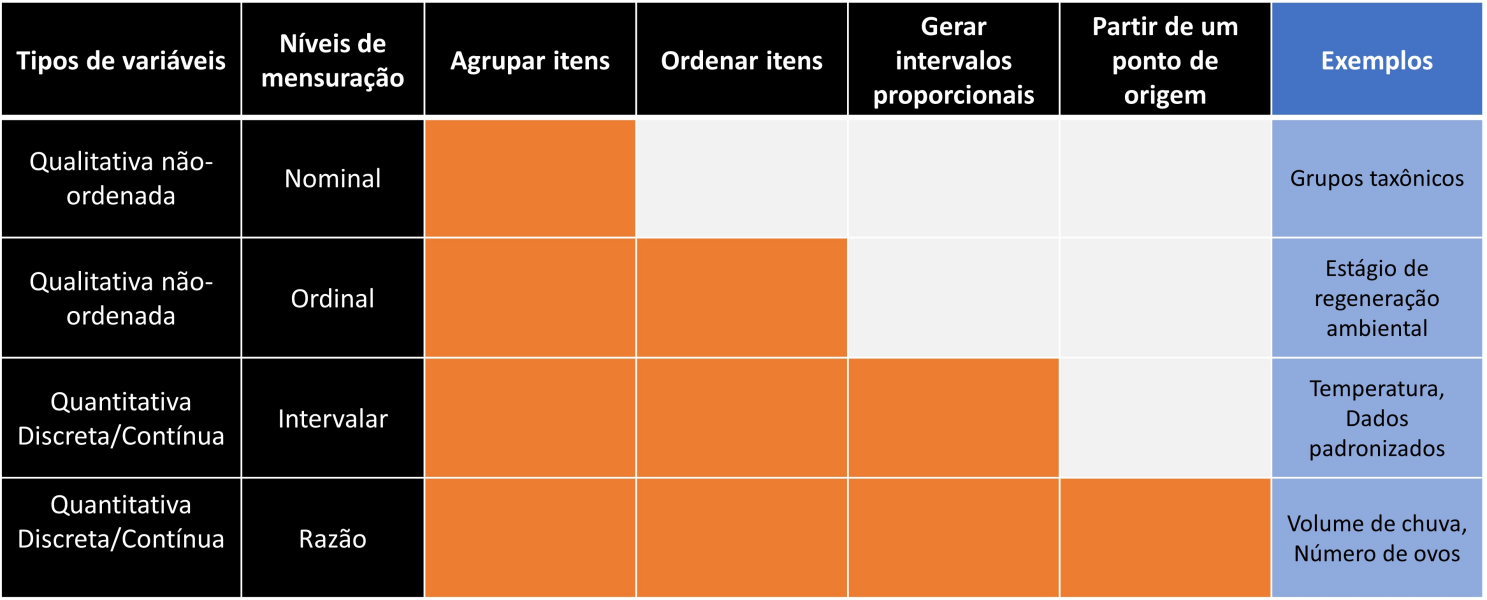
\includegraphics[width=20.65in]{probest-cambientais_files/figure-latex/unnamed-chunk-5-1} \end{center}

\hypertarget{proc_dados}{%
\chapter{Processamento de dados}\label{proc_dados}}

Tabelas de dados como a apresentada no capítulo @ref(estr\_dados) são normalmente armazenadas em planilhas eletrônicas. Os formatos mais comuns são arquivos do tipo \texttt{.xlsx}, \texttt{.csv}, \texttt{.txt} e mais recentemente planilhas em nuvem (ex. google sheets). Os programas para visualização e destes tipos de arquivos são apropriados para inserçao e armazenamendo de dados, mas apresentam limitações para o processamento, descrição e visualização de dados.

Neste capítulo iremos utilizar a linguagem estatística R e o ambiente de trabalho RStudio para aplicar algumas ações comuns ao processamento de dados inicial. O objetivo é que a base de dados original permaneca inalterada e que todo o processamento seja feito em uma versão da base de dados que será importada para o programa R. Isto evita que sejam feitas alterações equivocadas diretamente na base de dados resultando em perda da informação original.

\hypertarget{criando-seu-projeto-de-trabalho-no-rstudio}{%
\chapter{Criando seu projeto de trabalho no RStudio}\label{criando-seu-projeto-de-trabalho-no-rstudio}}

Se você utiliza o \href{https://rstudio.com/}{RStudio} com ambiente de trabalho para a linguagem R, o modo mais organizado de gerenciar suas análises é criando um \textbf{Projeto}. Você pode criar um projeto via menu: \texttt{File}. Na jeanela que se abrir escolha \texttt{New\ Project\ -\/-\textgreater{}\textgreater{}\ New\ Project}. Na janela \texttt{Directory\ name:} escreva o nome de seu projeto e na janela \texttt{Create\ a\ project\ as\ subdirectory\ of:} escolha o local em seu computador em que o projeto será criado e finalmente pressione \texttt{Create\ Project}.

Ao fazer isto, será criada dentro do diretório selecionado, uma pasta com o nome que você escolheu para o projeto. Dentro desta pasta você encontrará um arquivo com o nome de seu projeto e extensão \texttt{.Rproj}.

A partir deste momento, sempre que você for trabalhar neste projeto, abra o RStudio pressionando duas vezes o mouse sobre o arquivo \texttt{.Rproj}. Ao fazer isto, o R saberá em que local do computador estão os documentos relacionados a este projeto. Uma das vantagens em utilizar \emph{projetos} no R é tornar mais simples a organização de arquivos relacionados ao projeto. Deste modo, todas as base de dados bem como o material gerado (figuras, slides, arquivos \texttt{.pdf}, etc) podem ser organizados em sub-diretórios do projeto.

Vamos criar na pasta \emph{Documentos} um projeto denominado \texttt{Intro\_estatistica}. Após criar este projeto, vamos verificar se o R esta realmente direcionado à este local utilizando o comendo \texttt{getwd()}

\begin{Shaded}
\begin{Highlighting}[]
\FunctionTok{getwd}\NormalTok{()}
\end{Highlighting}
\end{Shaded}

\begin{Shaded}
\begin{Highlighting}[]
\FunctionTok{cat}\NormalTok{(}\StringTok{"[1] C:/Users/f\_cop/Documents/Intro\_estatistica"}\NormalTok{)}
\end{Highlighting}
\end{Shaded}

\begin{verbatim}
## [1] C:/Users/f_cop/Documents/Intro_estatistica
\end{verbatim}

\hypertarget{descrit}{%
\chapter{Apresentando informações em tabelas e gráficos}\label{descrit}}

Vamos analisar os dados provinientes de parte de um experimento em que foram comparadas as idades de cetáceos encontrados mortos na Espanha e Escócia. Para cada indivíduo, alguns dentes foram extraídos e seccionados. A idade destes animais foi então estimada a partir de 3 diferentes métodos de coloração. Estes dados estão na tabela Cetaceans.csv e foram extraídos originalmente de: \url{https://highstat.com/index.php/mixed-effects-models-and-extensions-in-ecology-with-r}.

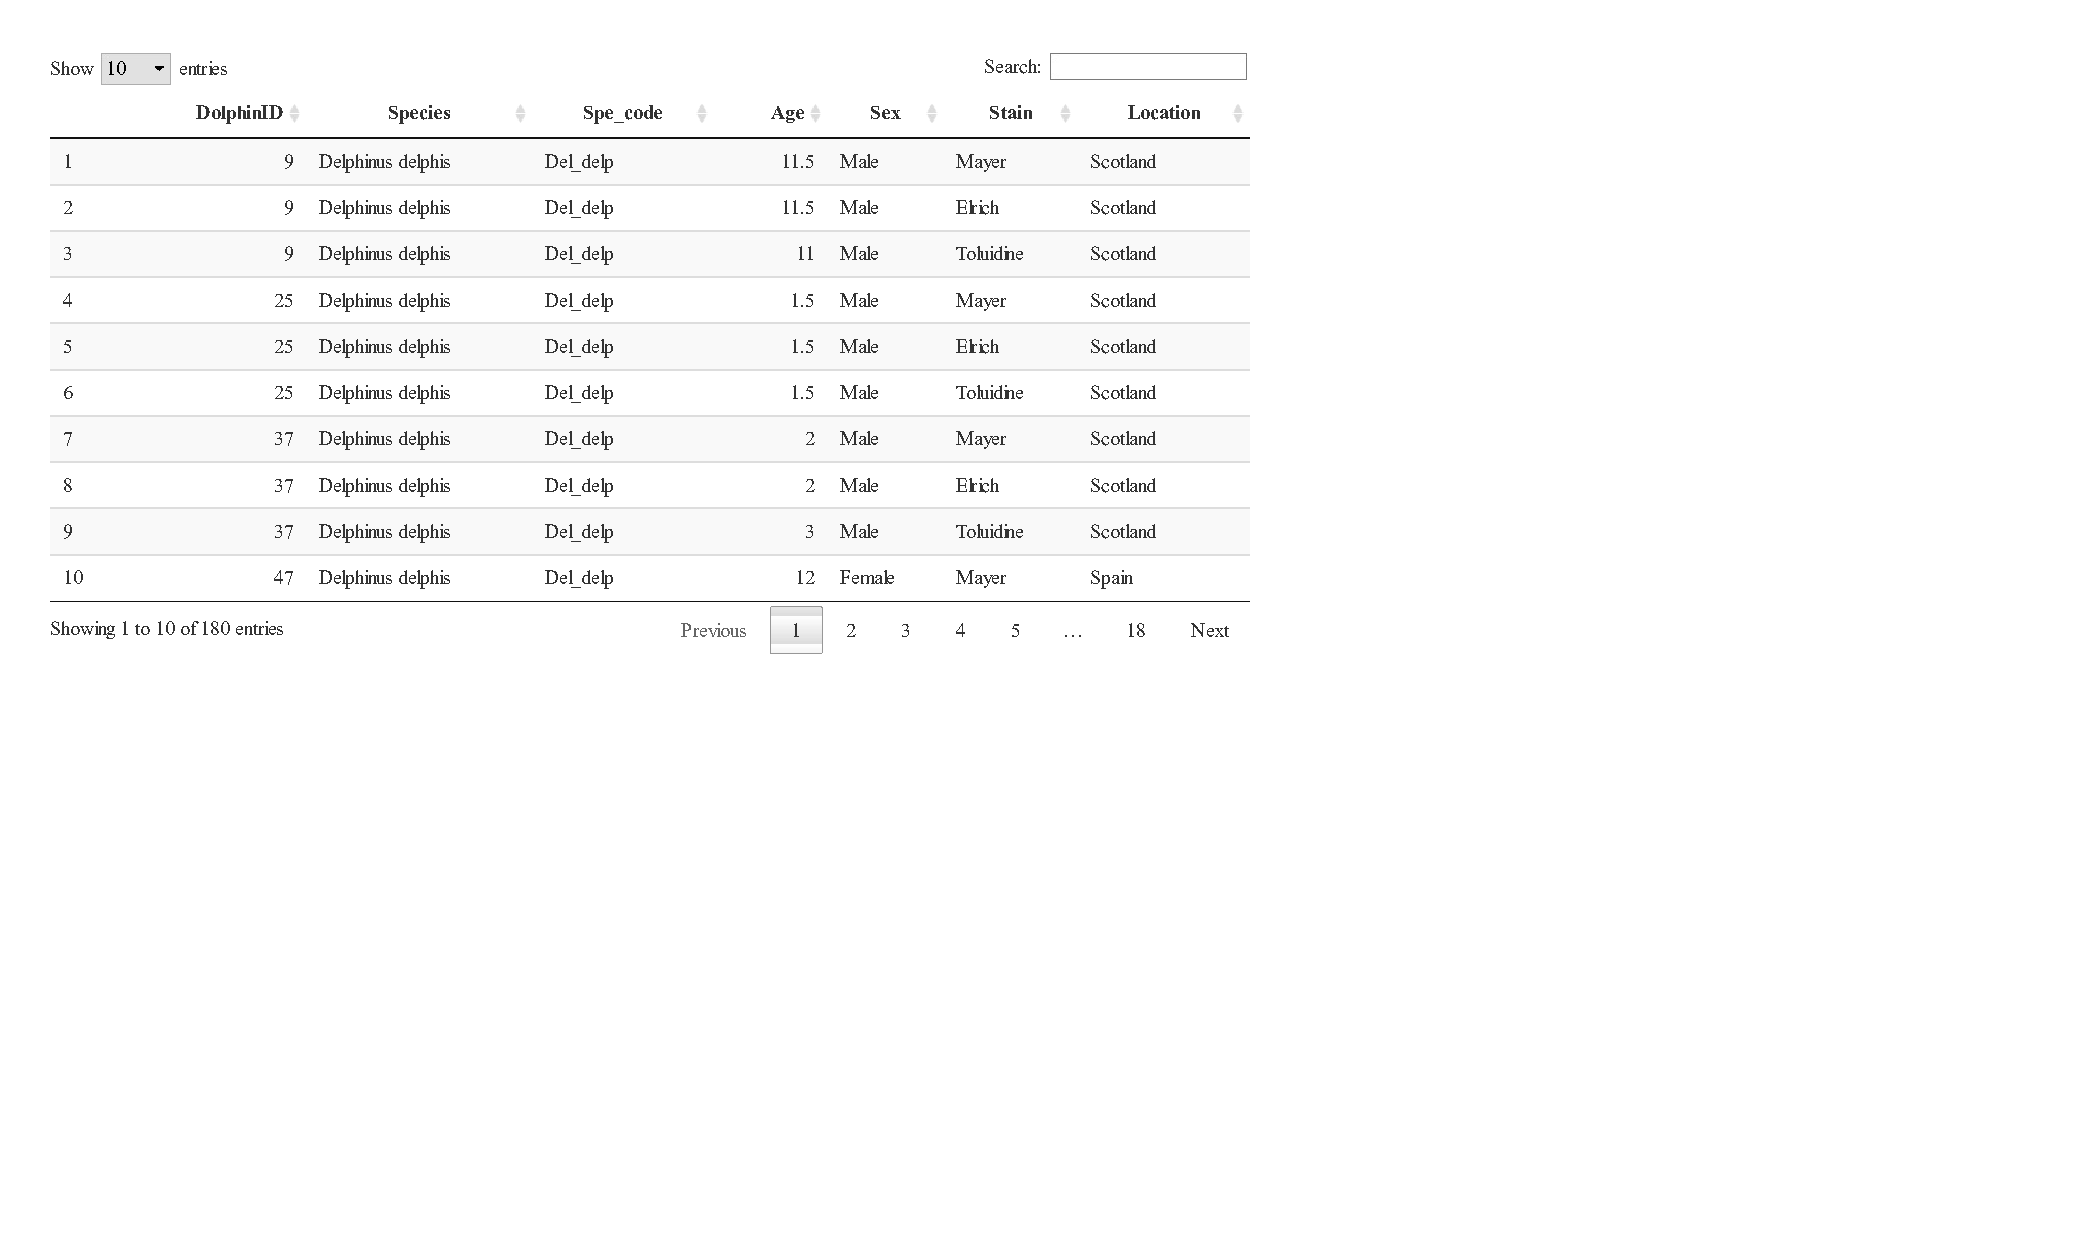
\includegraphics{probest-cambientais_files/figure-latex/unnamed-chunk-13-1.pdf}

A tabela contém 180 linhas por 7 colunas em que:

\textbf{DolphinID}: Identificação do indivíduo (61 indivíduos);

\textbf{Species}: Delphinus delphis, Lagenorhynchus acutus, Phocoena phocoena, Stenella coeruleoalba, Stenella frontalis, Tursiops truncatus;

\textbf{Age}: Idade do indivíduo;

\textbf{Sex}: Sexo (Female, Male, Unidentified);

\textbf{Stain}: Método de coloração (Elrich, Mayer, Toluidine);

\textbf{Location}: Local de captura (Scotland, Spain);

\hypertarget{tipos-de-dados-1}{%
\section{Tipos de dados}\label{tipos-de-dados-1}}

Métodos em estatística descritiva envolvem formas para visualizar, evidenciar e apresentar as informações mais relevantes de um conjunto de dados. Estes métodos aplicam, em grande parte, a construção de gráficos e tabelas apropriados a diferentes tipos de dados, além do cálculo de medidas de tendencia central (ex. média aritmética) e dispersão (ex. variância). Iremos discutir cada um destes tópicos neste e nos capítulos seguintes. O modo de visualização e apresentação depende da natureza dos dados. Estes pode ser basicamente de dois tipos: \textbf{quantitativos} ou \textbf{qualitativos}.

\hypertarget{dados-quantitativos-e-qualitativos}{%
\subsection{Dados quantitativos e qualitativos}\label{dados-quantitativos-e-qualitativos}}

Dados quantitativos são geralmente contagens (número de indivíduos, número de espécies, de carros, etc) ou mensurações (pesos, temperaturas, comprimentos, diversidade). Dados quantitativos podem ainda ser \textbf{discretos} ou \textbf{contínuos.} Dados discretos são representados por elementos enumeráveis. A contagem do número de pessoas em uma sala, do número de ovos em uma ninhada, número conchas no oceano. Dados discretos podem \textbf{somente} assumir valores inteiros (0, 1, 2,. . . ), ou seja, não existem valores fracionários como 1.5 pessoas, 2.5 conchas. Dados contínuos se referem a medidas que podem assumir infinitos valores, sem intervalos vazios. Pluviosidade, temperatura e pesos são alguns exemplos. A pluviosidade pode ser de 200 mm, 200.1 mm, 200.01 mm, 200.001 mm de chuva. O limite de precisão é aquele que podemos mensurar com os aparelhos disponíveis.

Dados qualitativos representam atributos ou categorias não numéricas (cor, profissão, tipos de vegetação).

\hypertarget{nuxedveis-de-mensurauxe7uxe3o-1}{%
\subsection{Níveis de mensuração}\label{nuxedveis-de-mensurauxe7uxe3o-1}}

Uma outra forma de organizar tipos de dados pode ser em função dos níveis de mensuração: \textbf{nominal}, \textbf{ordinal}, \textbf{intervalar} e \textbf{razão}.

\textbf{Nível nominal}: é característico de dados que possuem atributos ou categorias. Estes dados não podem ser ordenados. Ex. cor, grupo taxonômico, nomes de cidades, etc.

\textbf{Nível ordinal}: é aquele em que os atributos podem ser ordenados, embora não seja possível quantificar as diferenças entre dois níveis. Ex. i - Maratonistas podem ser classificados quanto à ordem de chegada em uma competição (1o; 2o; 3o; e assim por diante\ldots). ii - Cidades podem ser classificadas quanto às condições de saneamento: ótimo, bom, ruim, péssimo. iii - Pessoas podem ser ordenadas em ordem alfabética. No nível ordinal, não há sentido em quantificar as diferenças entre os níveis.

\textbf{Nível intervalar}: é aquele em que além ser possível ordenar, é possível quantificar as diferenças entre duas observações. No entanto, não há um ponto inicial natural, ou seja, um ponto zero que indique ausência da quantia. Ex. i -- Temperatura zero não indica ausência de temperatura, assim como dez graus não é duas vezes mais quente que 5 graus centígrados. Essas características são somente uma convenção relacionada à escala de mensuração da temperatura. ii - Ano do calendário: o ano zero é uma convenção do calendário, não significa ausência de tempo.

\textbf{Nível de razão}: é como o intervalar, porém existe um ponto zero natural. Peso igual a 0 kg indica ausência de peso e dez quilogramas é duas vezes mais pesado que 5 kg. O mesmo vale para comprimento, distância, velocidade, número de ovos. Existe uma relação entre tipo de dados e nível de mensuração. Da explicação acima, fica claro que os níveis nominal e ordinal se referem a dados qualitativos, enquanto os níveis intervalar e razão referem-se a dados quantitativos. Sempre é possível transformar dados quantitativos em qualitativos. Se temos os comprimentos em cm de peixes desembarcados (dados quantitativos, nível de mensuração razão), podemos transformá-los em atributos como peixes grandes e pequenos (qualitativo, nível de mensuração ordinal). Por outro lado, o contrário não é possível.

\hypertarget{tabelas-resumo}{%
\section{Tabelas resumo}\label{tabelas-resumo}}

No exemplo anterior, temos \texttt{Species}, \texttt{Stain}, \texttt{Sex} e \texttt{Location} como variáveis qualitativas nominais e \texttt{Age} como quantitativa contínua. A variável \texttt{DolphinID}, embora esteja codificada como um número entre 1 e 61, representa um \textbf{código de identificação} que não têm significado quantitativo, devendo desta forma, deve ser tratada como uma variável \textbf{categórica}.

A tabela de frequência a seguir mostra quantos dentes de cada espécie foram analisados.

\begin{tabular}{l|r}
\hline
Espécie & Frequência\\
\hline
Delphinus delphis & 21\\
\hline
Lagenorhynchus acutus & 9\\
\hline
Phocoena phocoena & 78\\
\hline
Stenella coeruleoalba & 27\\
\hline
Stenella frontalis & 27\\
\hline
Tursiops truncatus & 18\\
\hline
\end{tabular}

Esta tabela resume dados qualitativos, em que temos a contagem de cada um dos níveis da variável. Neste exemplo, temos a variável qualitativa \texttt{Species} com 6 níveis. Algumas espécies tiveram somente 9 dentes analizados e enquanto outras tiveram 78.

Podemos olhar também para a \textbf{frequência relativa} do número de dentes observados.

\begin{tabular}{l|r|r}
\hline
Espécie & Frequência & Frequência relativa\\
\hline
Delphinus delphis & 21 & 0.12\\
\hline
Lagenorhynchus acutus & 9 & 0.05\\
\hline
Phocoena phocoena & 78 & 0.43\\
\hline
Stenella coeruleoalba & 27 & 0.15\\
\hline
Stenella frontalis & 27 & 0.15\\
\hline
Tursiops truncatus & 18 & 0.10\\
\hline
\end{tabular}

Onde vemos que 43 \% dos dentes analizados pertencem a espécie Phocoena phocoena, enquanto somente 5 \% para Lagenorhynchus acutus. A frequência relativa nesta tabela deve somar 1.

Podemos analisar também a frequência de dentes analizados por região:

\begin{tabular}{l|r}
\hline
Região & Frequência\\
\hline
Scotland & 99\\
\hline
Spain & 81\\
\hline
\end{tabular}

A variável \texttt{Location} tem somente 2 categorias: Scotland e Spain.

\hypertarget{combinando-duas-variuxe1veis}{%
\subsection{Combinando duas variáveis}\label{combinando-duas-variuxe1veis}}

Vamos agora montar uma tabela de frequência para a combinação de duas variáveis categóricas, \texttt{Location} e \texttt{Species}.

\begin{tabular}{l|r|r}
\hline
Espécie & Scotland & Spain\\
\hline
Delphinus delphis & 9 & 12\\
\hline
Lagenorhynchus acutus & 9 & 0\\
\hline
Phocoena phocoena & 78 & 0\\
\hline
Stenella coeruleoalba & 3 & 24\\
\hline
Stenella frontalis & 0 & 27\\
\hline
Tursiops truncatus & 0 & 18\\
\hline
\end{tabular}

Podemos ver também suas \textbf{frequências relativas}. Neste caso temos três opções: calcular as frequências relativas \textbf{totais}, por \textbf{linhas} ou por \textbf{colunas}.

\hypertarget{frequuxeancias-relativas-totais}{%
\subsubsection{Frequências relativas totais}\label{frequuxeancias-relativas-totais}}

\begin{tabular}{l|r|r}
\hline
Espécie & Scotland & Spain\\
\hline
Delphinus delphis & 0.05 & 0.07\\
\hline
Lagenorhynchus acutus & 0.05 & 0.00\\
\hline
Phocoena phocoena & 0.43 & 0.00\\
\hline
Stenella coeruleoalba & 0.02 & 0.13\\
\hline
Stenella frontalis & 0.00 & 0.15\\
\hline
Tursiops truncatus & 0.00 & 0.10\\
\hline
\end{tabular}

Se estamos interessados nas frequências totais, cada célula deve ser dividida pela \textbf{soma total} da tabela, ou seja, 180. A célula 1, por exemplo, fica como 9 dividido por 180, e deste modo temos que 5\% dos dentes analisados eram de Delphinus delphis encontrados em Scotland. Neste tipo de tabela, a soma de \textbf{todas as células} deve somar 1.

\hypertarget{frequuxeancias-relativas-por-linhas}{%
\subsubsection{Frequências relativas por Linhas}\label{frequuxeancias-relativas-por-linhas}}

\begin{tabular}{l|r|r}
\hline
Espécie & Scotland & Spain\\
\hline
Delphinus delphis & 0.43 & 0.57\\
\hline
Lagenorhynchus acutus & 1.00 & 0.00\\
\hline
Phocoena phocoena & 1.00 & 0.00\\
\hline
Stenella coeruleoalba & 0.11 & 0.89\\
\hline
Stenella frontalis & 0.00 & 1.00\\
\hline
Tursiops truncatus & 0.00 & 1.00\\
\hline
\end{tabular}

Neste caso estamos interessados nos valores relativos para cada linha individual. Vemos por exemplo que dos 21 dentes analizados para Delphinus delphis, 43\% estão em Scotland e 57\% estão em Spain. Nesta tabela, as frequências \textbf{de cada linha} da tabela devem somar 1 enquanto o somatório das colunas nos dá as \textbf{frequências marginais} de \texttt{Location}.

\hypertarget{frequuxeancias-relativas-por-colunas}{%
\subsubsection{Frequências relativas por colunas}\label{frequuxeancias-relativas-por-colunas}}

\begin{tabular}{l|r|r}
\hline
Espécie & Scotland & Spain\\
\hline
Delphinus delphis & 0.09 & 0.15\\
\hline
Lagenorhynchus acutus & 0.09 & 0.00\\
\hline
Phocoena phocoena & 0.79 & 0.00\\
\hline
Stenella coeruleoalba & 0.03 & 0.30\\
\hline
Stenella frontalis & 0.00 & 0.33\\
\hline
Tursiops truncatus & 0.00 & 0.22\\
\hline
\end{tabular}

Esta opção é oposta à anterior. Estamos interessados nos valores relativos para cada coluna individual. Neste caso, as frequências \textbf{de cada coluna} da tabela devem somar 1 enquanto o somatorio das linhas nos dá as \textbf{frequências marginais} de \texttt{Species}.

\hypertarget{tabelas-de-frequuxeancia-para-variuxe1veis-quantitativas}{%
\subsection{Tabelas de frequência para variáveis quantitativas}\label{tabelas-de-frequuxeancia-para-variuxe1veis-quantitativas}}

Para variáveis quantitativas devemos primeiramente dividir a variável em \textbf{intervalos de classe}. Feito isto, contamos o número de observações dentro de cada classe. Vamos montar uma tabela de frequência para a variável \texttt{Age}. Temos idades variando entre 0 e 25 anos. Vamos então dividir este intervalo em 5 classes de tamanho 5.

\begin{tabular}{l|r}
\hline
Classe & Frequência\\
\hline
[0,5] & 97\\
\hline
(5,10] & 40\\
\hline
(10,15] & 27\\
\hline
(15,20] & 12\\
\hline
(20,25] & 4\\
\hline
\end{tabular}

A classe {[}0,5{]} tem o maior numero de dentes analisados (97 dentes) e a classe (20,25{]} o menor (4 dentes). Lembre-se que a variável \texttt{Age} é quantitativa. A divisão em classes de tamanho cinco foi uma escolha, de certa forma, arbitrária. Resumir uma dado quantitativo em intervalos de classe têm como objetivo principal destacar padrões no conjunto de dados.

Poderíamos escolher tamanhos de classe diferentes, por exemplo de tamanho 10 anos, o que nos daria um número muito pequeno de classes a ser analisada.

\begin{tabular}{l|r}
\hline
Classe & Frequência\\
\hline
[0,10] & 137\\
\hline
(10,20] & 39\\
\hline
(20,30] & 4\\
\hline
\end{tabular}

Poderíamos por outro lado, escolher um tamanho igual a dois, o que gera um número muito maior de classes.

\begin{tabular}{l|r}
\hline
Classe & Frequência\\
\hline
[0,2] & 82\\
\hline
(2,4] & 13\\
\hline
(4,6] & 3\\
\hline
(6,8] & 22\\
\hline
(8,10] & 17\\
\hline
(10,12] & 10\\
\hline
(12,14] & 11\\
\hline
(14,16] & 10\\
\hline
(16,18] & 5\\
\hline
(18,20] & 3\\
\hline
(22,24] & 3\\
\hline
(24,26] & 1\\
\hline
\end{tabular}

\hypertarget{frequuxeancias-acumuladas}{%
\subsubsection{Frequências acumuladas}\label{frequuxeancias-acumuladas}}

Uma vez que estamos trabalhando com uma variável quantivativa, faz sentido montar uma tabela de frequência acumulada, ou seja, vamos acumulando a frequências das classes inferiores à medida que avançamos para as classes maiores. No exemplo acima, uma tabela de frequência acumulada ficaria:

\begin{tabular}{l|r|r}
\hline
Classe & Frequência & Frequência acumulada\\
\hline
[0,5] & 97 & 97\\
\hline
(5,10] & 40 & 137\\
\hline
(10,15] & 27 & 164\\
\hline
(15,20] & 12 & 176\\
\hline
(20,25] & 4 & 180\\
\hline
\end{tabular}

Nesta tabela, a \(2^a\) linha da coluna de frequência acumulada é o somatório da \(1^a\) e da \(2^a\) da coluna de frequências. À medida que descemos nas linhas, vamos somando as frequências das classes inferiores. Deste modo, a última linha da coluna de frequências acumuladas nos dá o número total de observações na tabela, neste exemplo, 180 observações.

Podemos construir uma tabela similar utilizando os dados de frequência relativa. Neste caso, a última linha deve somar 1 como visto abaixo.

\begin{tabular}{r|r}
\hline
Frequência & Frequência acumulada\\
\hline
0.54 & 0.54\\
\hline
0.22 & 0.76\\
\hline
0.15 & 0.91\\
\hline
0.07 & 0.98\\
\hline
0.02 & 1.00\\
\hline
\end{tabular}

\hypertarget{visualizauxe7uxe3o-gruxe1fica}{%
\section{Visualização gráfica}\label{visualizauxe7uxe3o-gruxe1fica}}

A forma de representação gráfica depende o tipo (qualitativa ou quantitativa) e do número de variáveis envolvidas na análise. Em geral temos 5 tipos básicos de gráficos utilizados em análise e interpretalção de dados, \textbf{gráficos de barras}, \textbf{histogramas}, \textbf{gráficos de linhas}, \textbf{gráficos de dispersão} e \textbf{boxplots}. Vamos apresentar os quatro primeiros nesta seção e deixar a discussão dos boxplots para o capítulo \ref{posicao} quando abordarmos \textbf{distribuições de frequência}, \textbf{medidas de tendência central}, \textbf{posição} e \textbf{variação}.

\hypertarget{gruxe1ficos-de-barras}{%
\subsection{Gráficos de barras}\label{gruxe1ficos-de-barras}}

Considere novamente os dados da tabela \texttt{Cetaceans.csv} apresentada no início do capítulo.

Um gráfico de barras é utilizado para representar variáveis qualitativas. O gráfico de barras nos permite mostar as mesmas informações contidas nas \textbf{tabelas de frequência}. Cada barra representa a contagem ou a frequência relativa dos níveis da variável.

Neste exemplo, vamos representar o número de dentes analisados em função do sexo de animal. Nas figuras abaixo, vemos um número maior de machos e alguns poucos indivíduos com sexo não identificado.

\begin{center}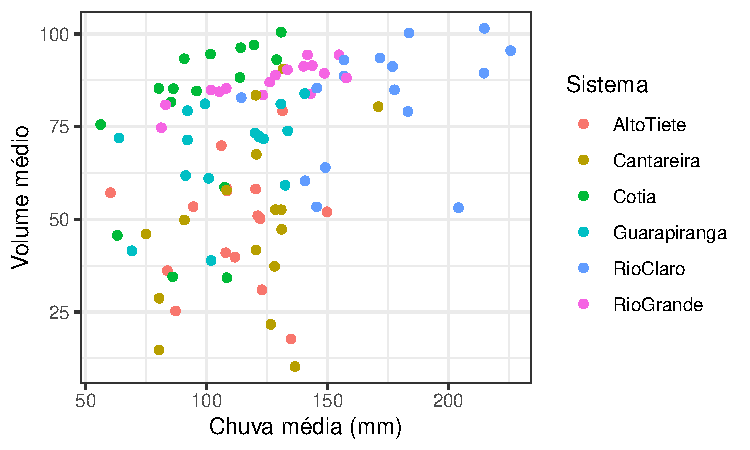
\includegraphics{probest-cambientais_files/figure-latex/unnamed-chunk-26-1} \end{center}

Os gráficos de barras apresentados acima descrevem o padrão observado para \textbf{somente uma} variável qualitativa. Podemos no entanto, utilizá-lo também para verificar a associação entre \textbf{duas} variáveis qualidativas. Abaixo, é descrita a abundância relativa por sexo para \textbf{cada uma} das localidades.

\begin{center}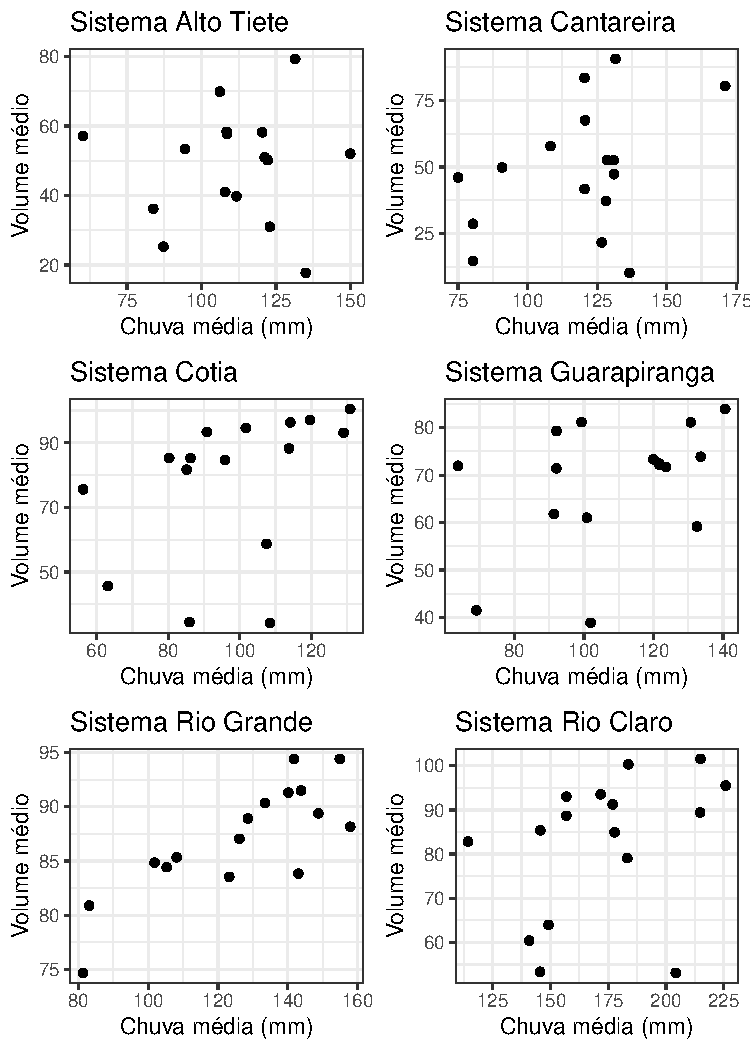
\includegraphics{probest-cambientais_files/figure-latex/unnamed-chunk-27-1} \end{center}

Quando combinamos duas variáveis qualitativas no mesmo gráfico de barras, podemos organizá-las de duas formas. Na figura da esquerda agrupamos as abundâncias das duas localidades lado a lado para cada um dos sexos. Na figura da direita, agrupamos os sexos e separamos as localidades. Compare as duas figuras. Veja que as duas mostram as mesmas informações. Entretanto, a escolha entre elas irá depender do objetivo do trabalho e das relações que desejamos tornar mais clara ao leitor.

\hypertarget{histogramas}{%
\subsection{Histogramas}\label{histogramas}}

Histogramas são utilizados para representar o padrão de distribuição de dados quantitativos, semelhante ao que fizemos com com a \textbf{tabela de frequência de classes}. Para isto também é necessário dividir a variável em \textbf{intervalos de classes}. Portanto, os histogramas mostram as mesmas informações que obtivemos nas tabelas de frequência para variáveis quantitativas.

Intervalos de classes muito amplos, causam muita perda de informação a respeito da distribuição de valores, enquanto intervalos muito estreitos, são demasiadamente detalhados e dificultam a visualização de um padrão geral. Abaixo apresentamos histogramas para a variável \texttt{Age} com três intervalos de classes distintos (10, 5, e 1 anos). Deste modo, todos expressam as mesmas informações em níveis de detalhes cada vez maiores à medida que reduzimos o intervalo de classe.

\begin{center}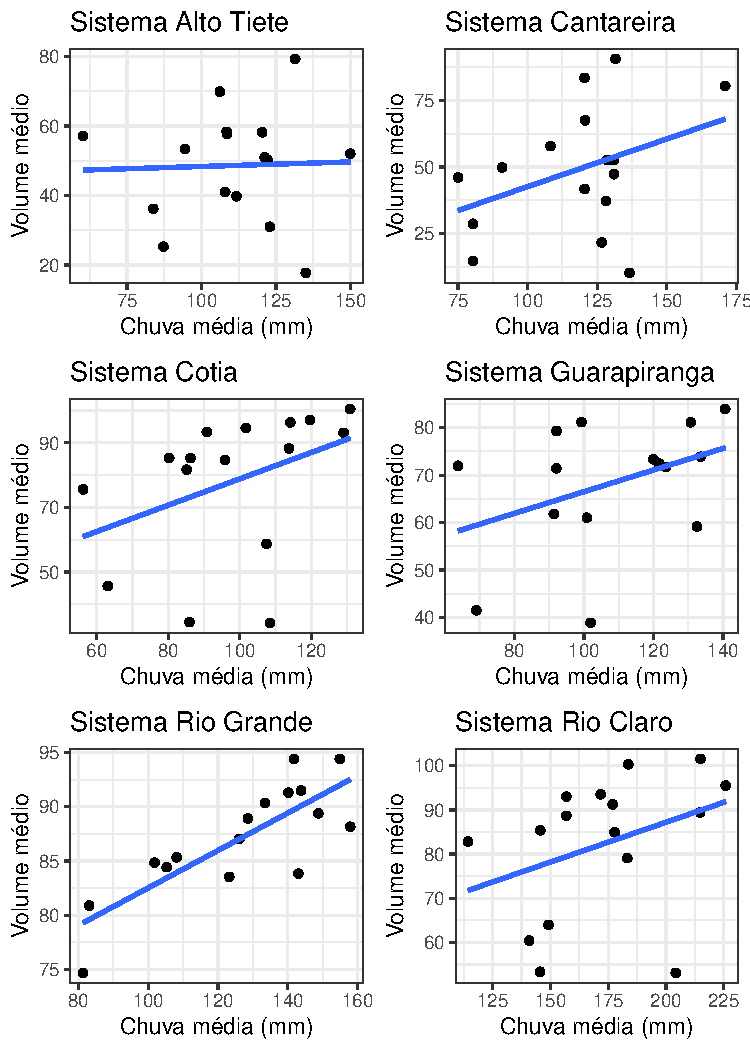
\includegraphics{probest-cambientais_files/figure-latex/unnamed-chunk-28-1} \end{center}

\hypertarget{gruxe1ficos-de-linhas}{%
\subsection{Gráficos de linhas}\label{gruxe1ficos-de-linhas}}

Um gráfico de linhas pode ser utilizado quando há uma ordem inerente ao conjunto de dados. Este tipo de dados é comumente visto para representar \textbf{séries temporais}, em que as medidas são tomadas ao longo do tempo. Na tabela abaixo, por exemplo, estão representados os volumes de chuva e níveis de água (média do ano) em seis sistemas de abastecimento de água da Grande São Paulo (Alto Tietê, Cantareira, Cotia, Guarapiranga, Rio Claro e Rio Grande). Os dados foram medidos entre 2003 e 2018. A tabela possui 96 linhas por 4 colunas. Cada linha representa as medidas tomadas em um dos sistemas e em cada um dos anos considerados.

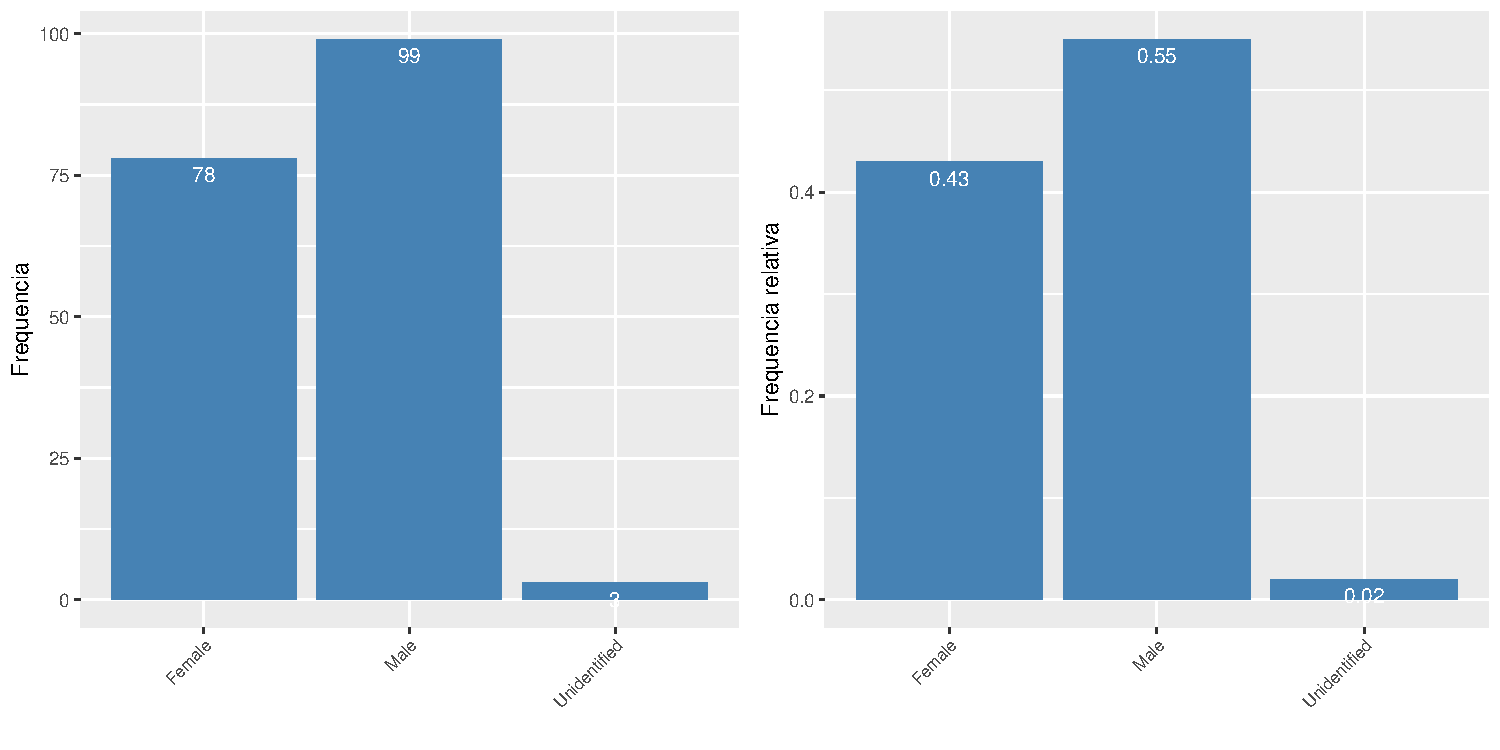
\includegraphics{probest-cambientais_files/figure-latex/unnamed-chunk-29-1.pdf}

A figura a seguir representa a variação anual no volume médio para o Sistema Cantareira, onde podemos perceber um aumento no volume em 2010, seguido de uma redução que atinge seu pico mínimo em 2015.

\begin{center}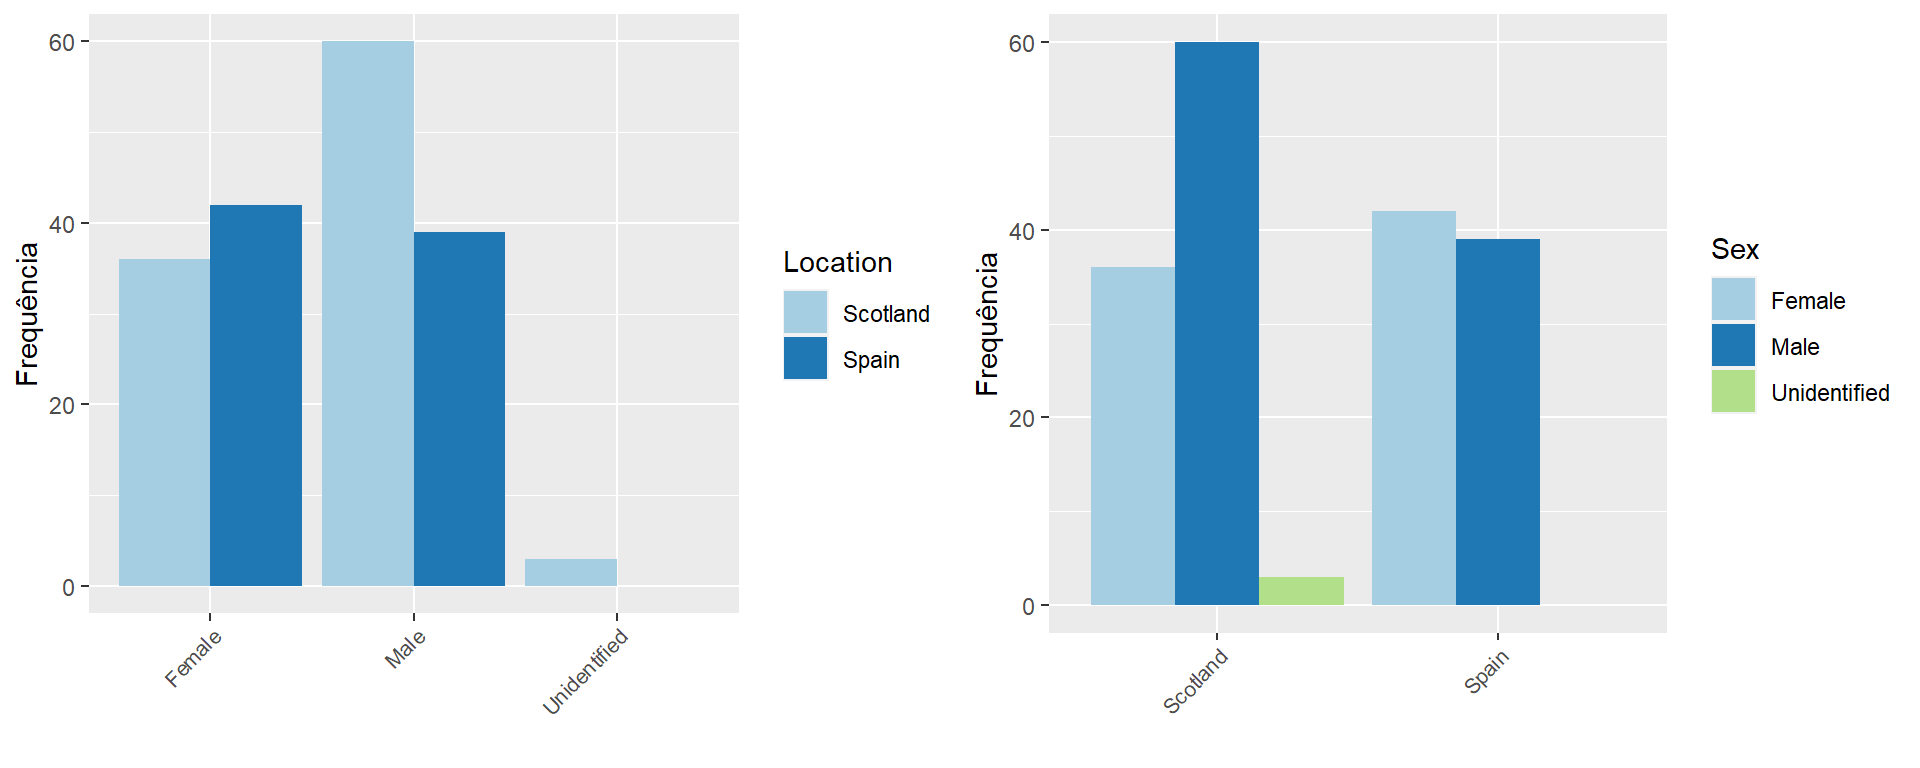
\includegraphics{probest-cambientais_files/figure-latex/unnamed-chunk-30-1} \end{center}

Na figura anterior, verificamos a relação entre duas variáveis (Ano e Volume médio) \textbf{exclusivamente} para o sistema Cantareira.

Podemos utiliar o mesmo tipo de gráfico para associar três variáveis ao mesmo tempo: Ano, Volume médio e Sistema de abastecimento. A variável Sistema de Abastecimento é categórica e possui 6 níveis. Vamos inicialmente representar os sistemas Cantareira, na zona Norte da Grande São Paulo, e o Sistema Rio Grande na zona Sul. Podemos perceber que os padrões são distintos. O sistema Rio Grande parece manter um volume maior, ao redor de 80, enquanto o sisterma Cantareira, fica ao redor de 50. A \textbf{variação}, descrita pela diferênça entre os picos máximo (em 2010) e mínimo (em 2015), é maior no Sistema Cantareira. Em resumo esta figura sugere que nos últimos 15 anos, o volume médio no Sistema Rio Gande foi mais elevado e mais estável que no Sistema Cantareira.

\begin{center}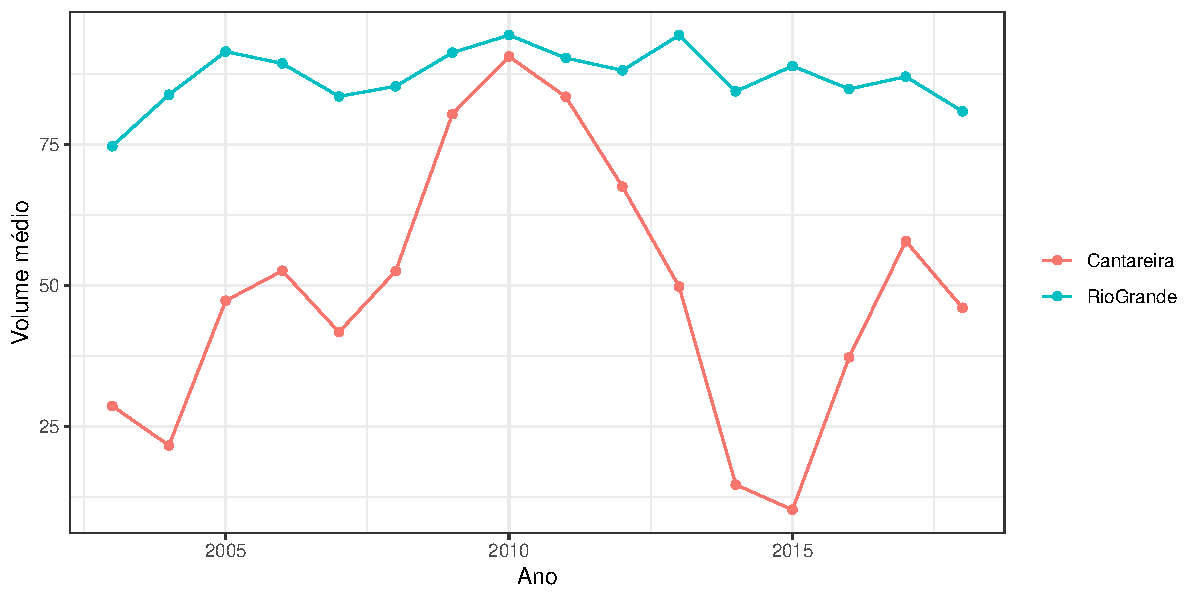
\includegraphics{probest-cambientais_files/figure-latex/unnamed-chunk-31-1} \end{center}

Vamos olhar para todos os sistemas juntos. Um dos objetivos da análise gráfica, é encontrarmos padrões comuns, tendências gerais que se repetem para grupos diferentes. Na figura anterior, existem \textbf{aparentemente} três padrões distintos. Os sistemas Cantareira e Alto Tietê mantém níveis mais baixos e também mais variáveis, enquanto os sistemas Rio Claro e Rio Grande mantiveram níveis mais elevados e mais estáveis. Finalmente, os sistemas Cotia e Guarapiranga parecem apresentar padrões intermediários.

\begin{center}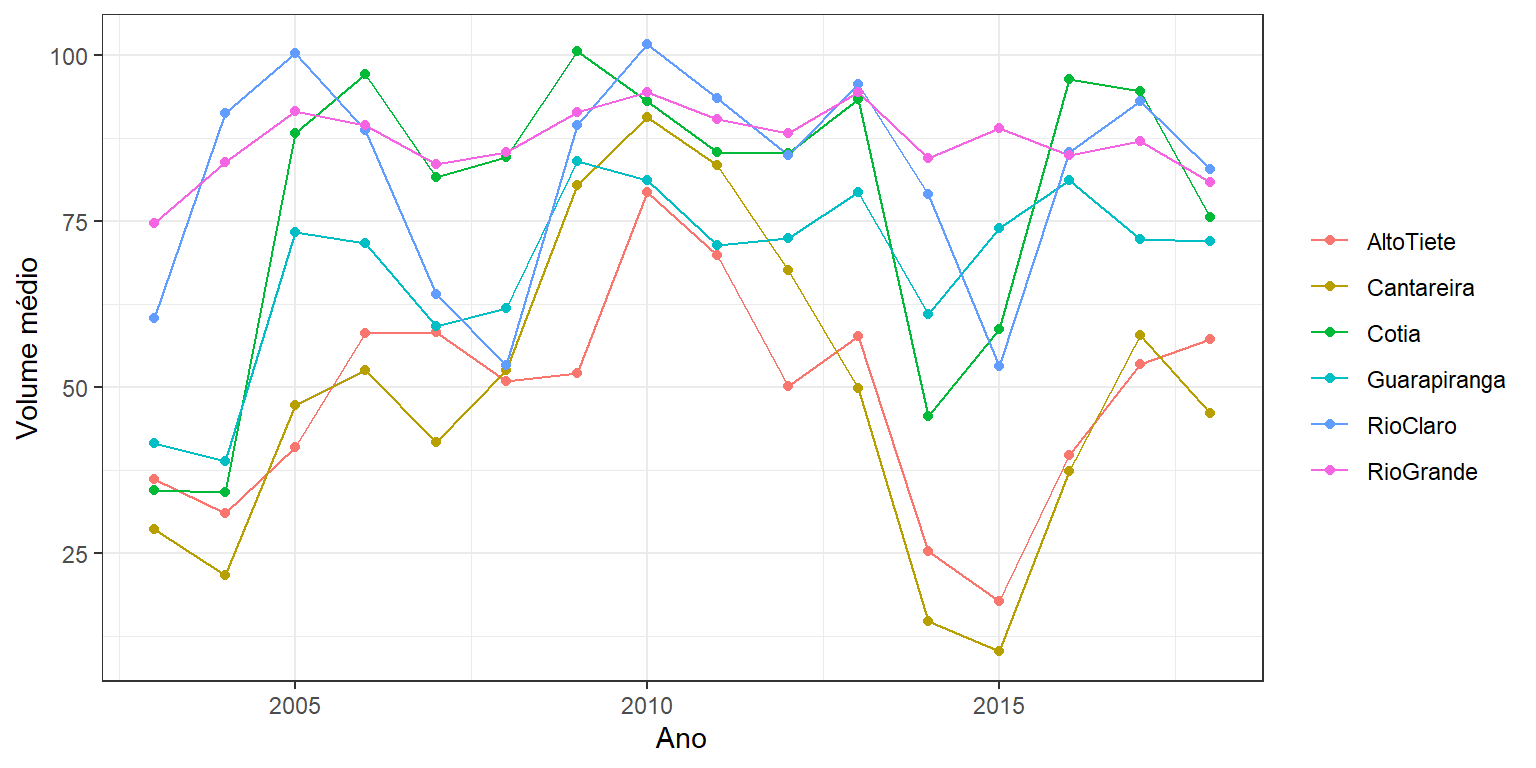
\includegraphics{probest-cambientais_files/figure-latex/unnamed-chunk-32-1} \end{center}

Vamos olhar para cada um dos grupos sugeridos em figuras separadas.

\begin{center}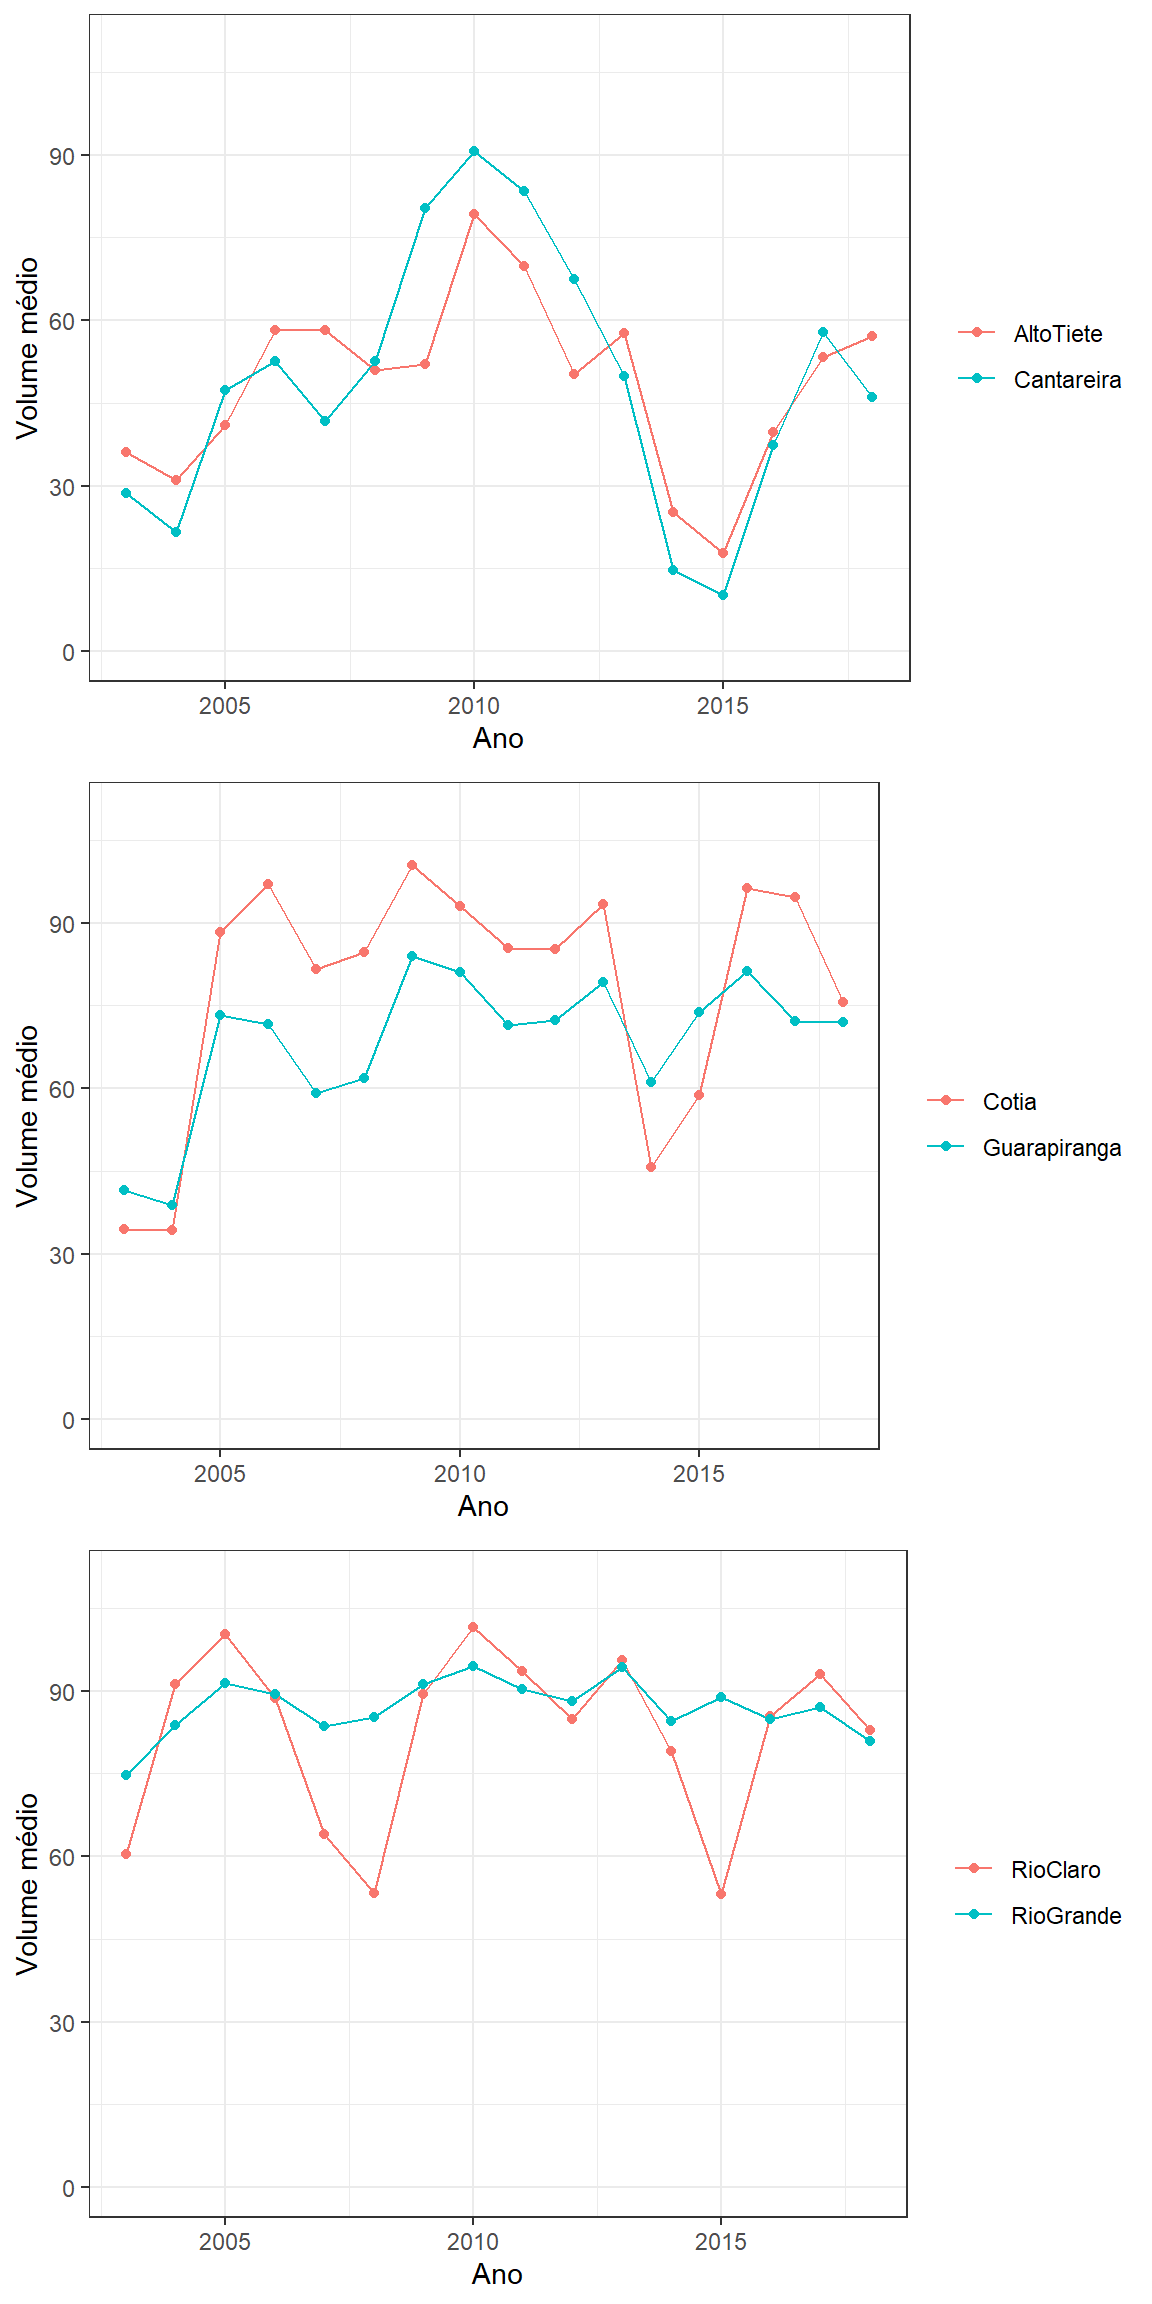
\includegraphics{probest-cambientais_files/figure-latex/unnamed-chunk-33-1} \end{center}

Esta é somente, uma avaliação superficial e exploratória. Poderíamos pensar em causas (\textbf{hipóteses}) que explicassem estes padrões aparentes como clima regional, geomeorfologia da áreas, dinâmica de vazão dos rios que abastecem o sistema, política de uso água, número de pessoas abastecidas, etc\ldots{} Neste caso, estaríamos entrando no campo da \textbf{Inferência Estatística}.

\hypertarget{gruxe1ficos-de-dispersuxe3o}{%
\subsection{Gráficos de dispersão}\label{gruxe1ficos-de-dispersuxe3o}}

Gráficos de dispersão são utilizados para associar duas variáveis quantitativas entre si. Ao contrário do gráfico de linhas, não é necessário que exista qualquer ordem inderente no conjunto de dados. Vamos verificar por exemplo a relação entre volume médio anual e a chuva média anual entre 2003 e 2018.

\begin{center}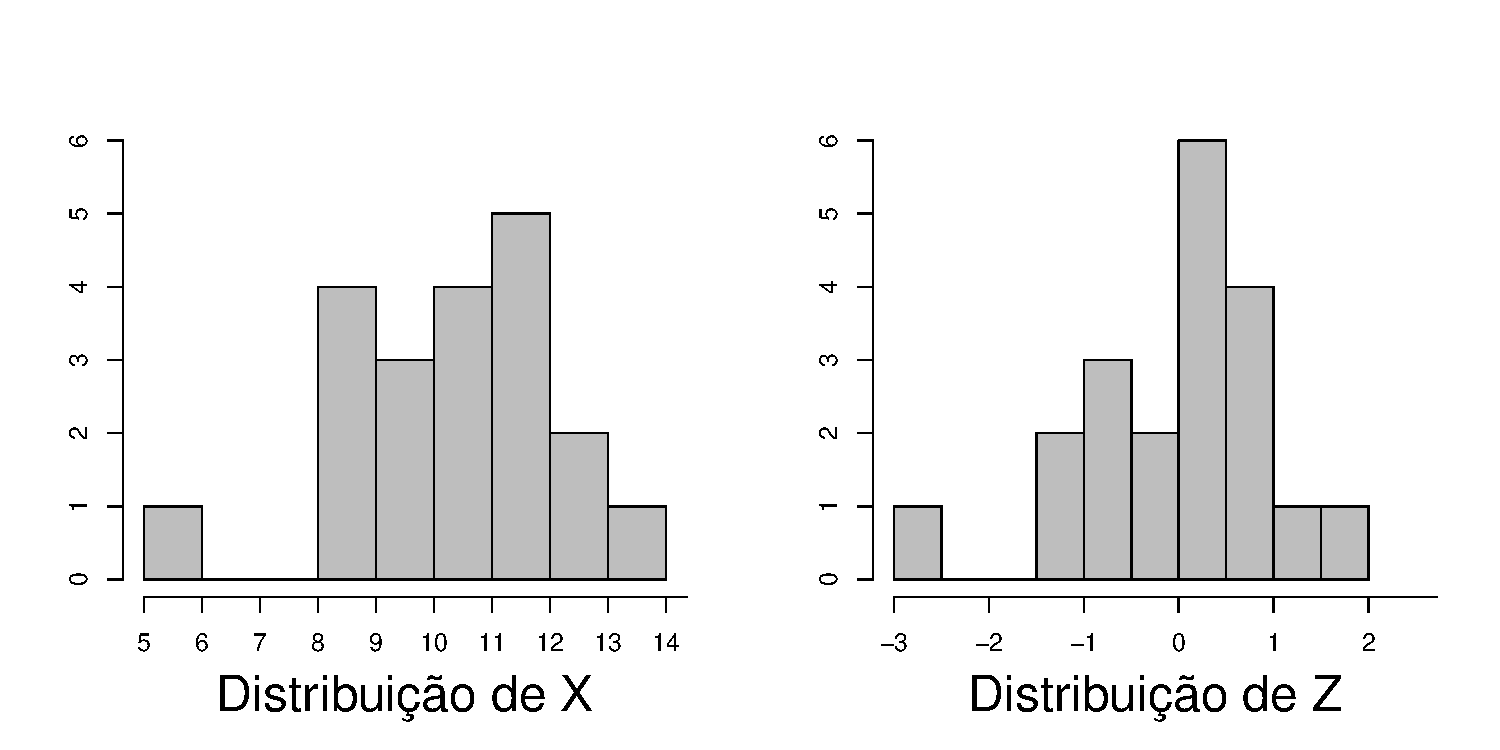
\includegraphics{probest-cambientais_files/figure-latex/unnamed-chunk-34-1} \end{center}

Não parece haver uma relação muito clara, o que é curioso. Como os sistemas são abastecidos pelos rios que drenam suas regiões, esperaríamos que anos de muita chuva, ressultassem em reservatórios com níveis mais elevados.

Entretanto, vimos no tópico anterior que os reservatório apresentaram diferenças nos padrões de variação do volume médio anual. Vamos verificar agora se eles também diferem na \textbf{relação} entre o volume de chuva e nível dos sistemas. Para explorarmos esta questão, vamos inserir uma \(3^a\) variável a figura (o sistema de abastecimento) como diferentes cores.

\begin{center}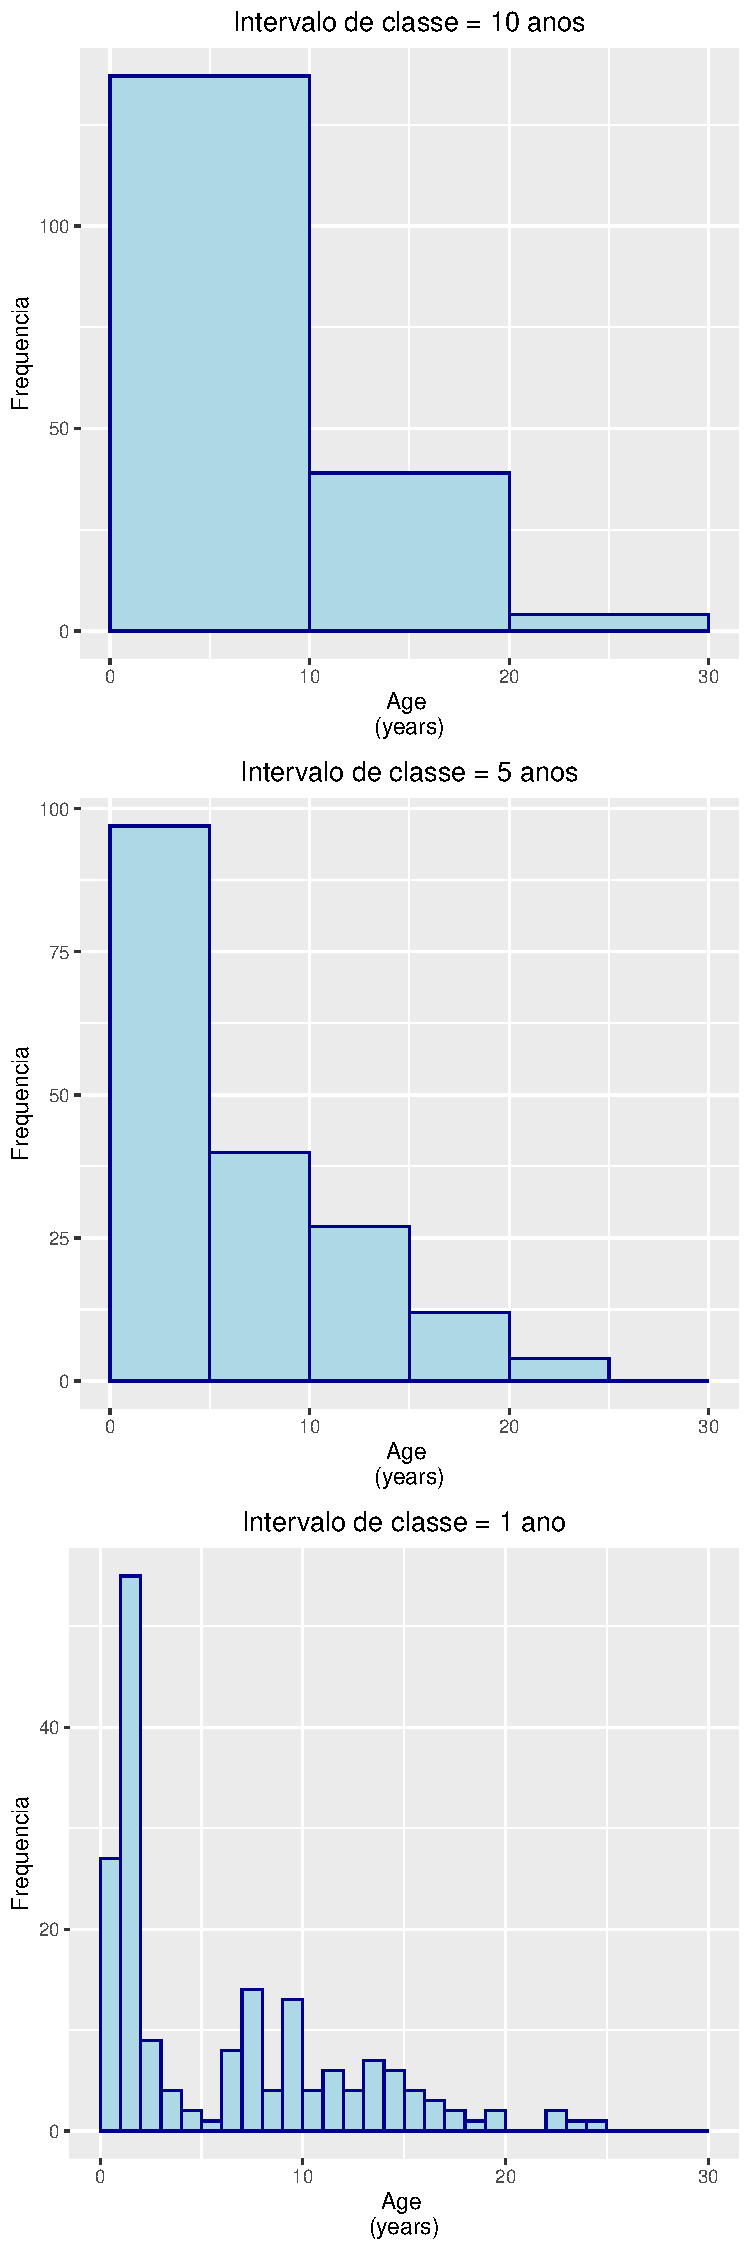
\includegraphics{probest-cambientais_files/figure-latex/unnamed-chunk-35-1} \end{center}

Como o número de curvas na figura dificulta a visualização de um padrão mais claro, vamos olhar para cada sistema \textbf{separadamente}.

\begin{center}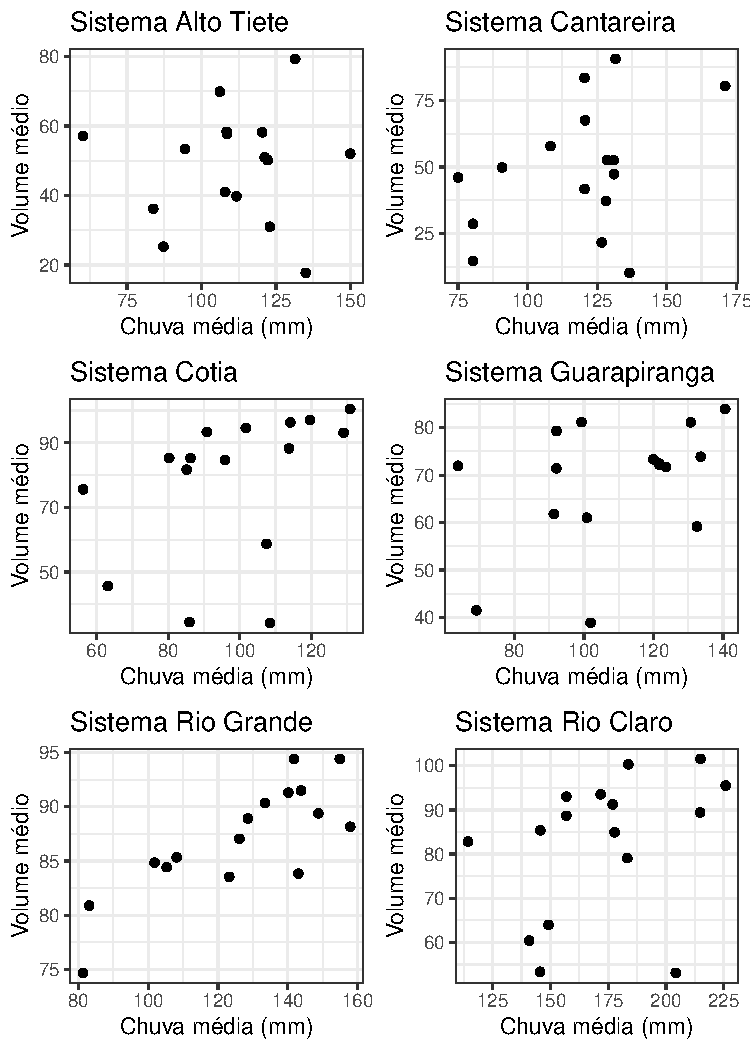
\includegraphics{probest-cambientais_files/figure-latex/unnamed-chunk-36-1} \end{center}

Separadamente podemos ver que parece haver uma \textbf{correlação positiva} entre volume de chuva e nível para o Sistema Rio Grande e, \emph{possivelmente}, para os Sistema Rio Claro. Aparentemente, estes sistemas se mantiveram mais cheios em anos mais chuvosos. Esta relação não parece existir para o sistema do Alto Tietê e é menos clara para os demais sistemas. Podemos explorar melhor esta questão inserindo uma \textbf{linha de regressão}.

\begin{center}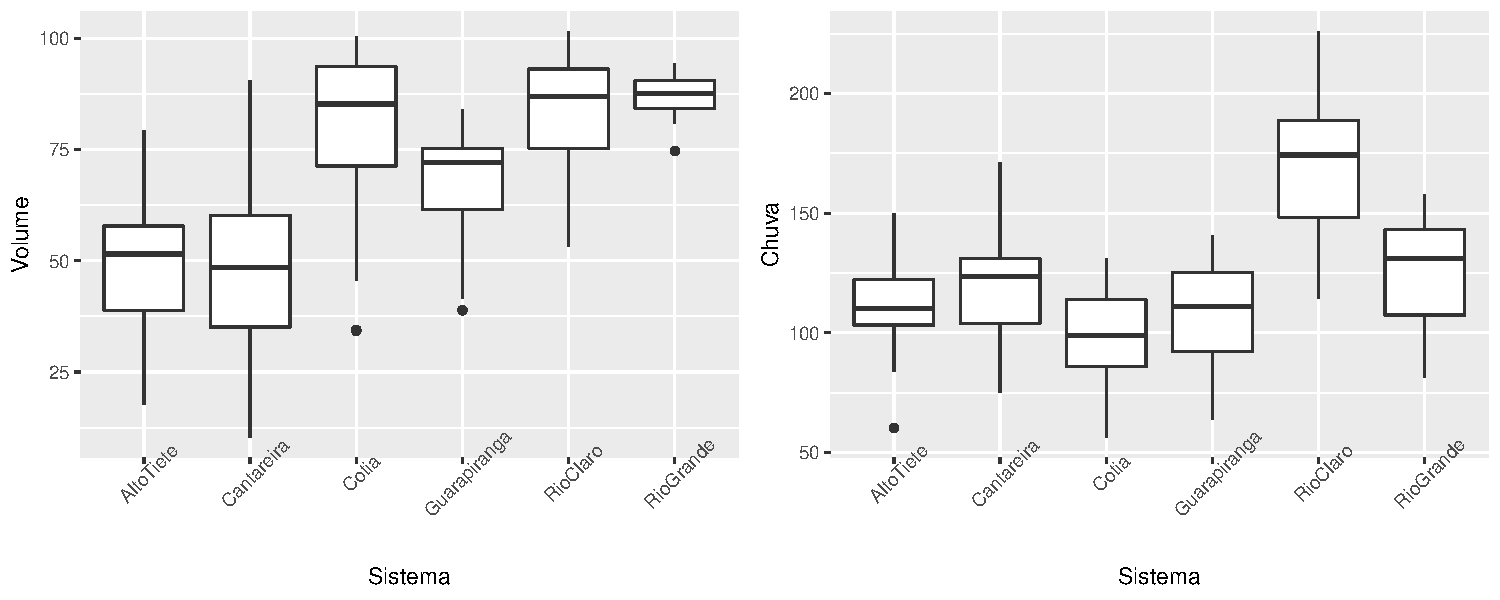
\includegraphics{probest-cambientais_files/figure-latex/unnamed-chunk-37-1} \end{center}

As linhas nos sugerem que para todos os sistemas, há uma relação \textbf{positiva} entre o volume do reservatório e o volume médio de chuva anual, \textbf{exceto} para o sistema do Alto Tietê. Neste sistema a relação parece nula, o que é uma questão interessante em se estudar! Iremos estudar o método de \textbf{regressão linear} no capítulo \ref{th}.

\hypertarget{posicao}{%
\chapter{Descrevendo populações e amostras}\label{posicao}}

\hypertarget{populauxe7uxe3o-amostra-e-unidade-amostral}{%
\section{População, amostra e unidade amostral}\label{populauxe7uxe3o-amostra-e-unidade-amostral}}

Em estatística, \textbf{população} se refere a todos os elementos sobre os quais queremos tirar conclusões. É comum a confusão entre os termos população estatística e população biológica (nas ciências naturais) ou população humana (em ciências sociais). No entanto, \textbf{população estatística} refere-se ao \textbf{conjunto de medidas} que podem ser obtidas como resultado de um experimento ou de um estudo observacional e não pode ser confundido com conjuntos de pessoas ou organismos. As medidas que compõem a população estatística portanto, podem ser pesos, temperaturas, velocidades, tempos de reação, entre outras, a depender das características de um estudo particula. A abrangência da população estatística depende do contexto e do escopo da pergunta que se pretende responder.

Suponha um estudo para descrever o comprimento do lambari \emph{Deuterodon iguape} em riachos do litoral de São Paulo. A população estatística não são os peixes em si, mas o \textbf{comprimento} de cada indivíduo. Dado o escopo do estudo, a população estatística abrange \textbf{somente} comprimentos dos organismos que habitam bacias do litoral de São Paulo. Suponha agora que desejamos estudar a diversidade de espécies de peixes em bacias costeiras do litoral de São Paulo. Neste caso, a população estatística seria constituida de um \textbf{índice de diversidade} calculado para cada uma das bacias costeiras do litoral. Fica claro que, neste caso, população estatística não tem qualquer relação com população biológica, mas sim com uma medida obtida do conjunto de espécies que habitam cada bacia.

Nos dois exemplos acima é inviável obtermos informações de todos os elementos que compõem a população estaística. Para o exemplo dos comprimento, temos provavelmente alguns milhares de peixes na Bacia e consequentemente, o mesmo número de comprimentos individuais. O número de Bacias costeiras no litoral do Estado de São Paulo é bem menor, porém ainda é inviável mensurar a diversidade de espécies em todas elas. Um \textbf{censo} ocorre nos raros exemplos em que é possível mensurar todos os elementos da população estatística. Entretanto, a prática em estatística lida com a maioria dos casos em que mensuramos um \textbf{subconjunto} da população estatística, definido como uma \textbf{amostra}.

Finalmente, \textbf{unidade amostral} é definida como um \textbf{único} elemento da população estatística. A unidade amostral deve ser a menor unidade \textbf{independente} associada ao estudo. A necessidade das unidades amostrais constituirem elementos independentes é um dos pressupostos centrais da estatística e suas implicações ficarão mais claras quando tratarmos do processo de amostragem. No exemplo dos lambaris, unidade amostral é o comprimento mensurado em um indivíduo da espécies de interesse, enquanto no exemplo das bacias costeiras, as unidades amostrais são cada os valores de diversidade calculado para cada bacia.

\begin{quote}
\textbf{População estatística}: todos os elementos que podem compor uma amostra. Podem ser medidas como comprimentos, temperaturas, velocidades, etc.
\end{quote}

\begin{quote}
\textbf{Unidade amostral}: um único elemento da população.
\end{quote}

\begin{quote}
\textbf{Censo}: o levantamento de \emph{todos} os elementos da população.
\end{quote}

\begin{quote}
\textbf{Amostra}: um subconjunto extraído da população.
\end{quote}

\begin{quote}
\textbf{Tamanho populacional} (\emph{N}): o número de elementos da população.
\end{quote}

\begin{quote}
\textbf{Tamanho amostral} (\emph{n}): o número de elementos da amostra.
\end{quote}

\hypertarget{distribuiuxe7uxf5es-de-frequuxeancia}{%
\section{Distribuições de frequência}\label{distribuiuxe7uxf5es-de-frequuxeancia}}

Os valores da população estatística não são idênticos. Os lambaris do exemplo anterior não têm todos o mesmo comprimento, assim como a diversidade de espécies não é a mesma para todas as bacias costeiras do estado de São Paulo. Dizemos que existe uma \textbf{distribuição} de valores. Os comprimentos de \emph{Deuterodon iguape} devem variar de alguns milímetros (pós-larva) a cerca de 20 cm (adulto). Da mesma forma, nem todos os comprimentos são igaulente representados. Provavelmente existem mais lambaris pequenos e médios que grandes. Se fosse possível observar todos os elementos da população estatística, poderíamos organizá-los em uma \textbf{distribuição de frequências}, onde veríamos que algumas classes de valores são mais comuns que outras.

\begin{figure}

{\centering 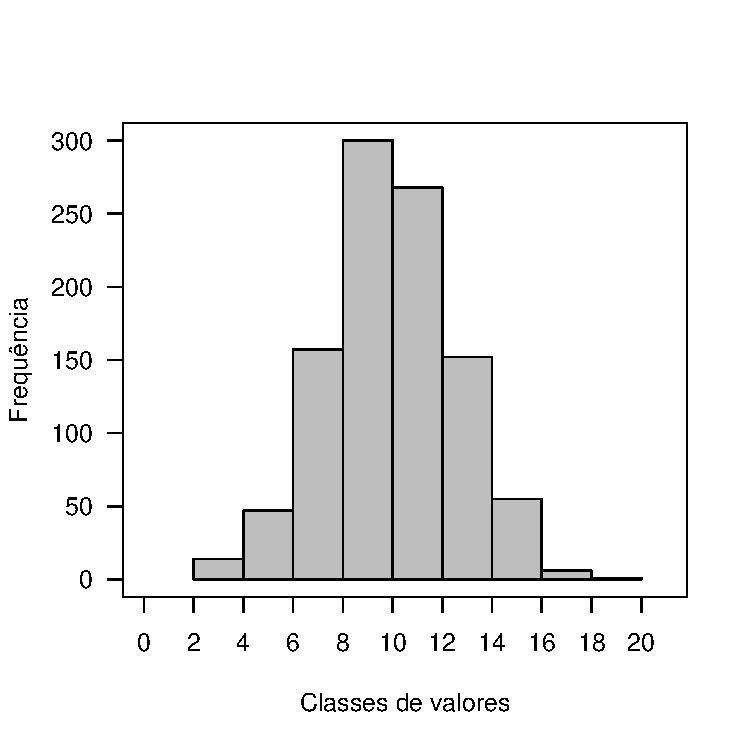
\includegraphics{probest-cambientais_files/figure-latex/distrfreq-1} 

}

\caption{Distribuição de frequência seguindo um modelo Gaussiano}\label{fig:distrfreq}
\end{figure}

Vemos que existem mais valores entre 8 e 12 por exemplo, e poucas observações extremas.

Este exemplo é fictício e segue uma \textbf{distribuição normal} de probabilidades. A distribuição normal, é uma das mais importantes em estatística. É uma distribuição \textbf{simétrica}, ou seja, os valores extremos são igualmente representados acima e abaixo da região central (média), apresenta uma forma de sino e também é chamada de distribuição \textbf{Gaussiana} em homenagem a \href{https://en.wikipedia.org/wiki/Carl_Friedrich_Gauss}{Carl Friedrich Gauss} um dos mais importantes matemáticos do século XXI. Gauss lidou com a distribuição normal quando desenvolveu a \textbf{Teoria da distribuição dos erros observacionais}, tópico central ao desenvolvimento da estatística e do método científico.

A distribuição normal será estudada em detalhes nos tópicos de inferência estatística e probabilidade. Voltaremos a ela também após falarmos dos descritores de tendêncoia central, posição e variação e de amostragem.

\hypertarget{paruxe2metros-e-estimadores}{%
\section{Parâmetros e estimadores}\label{paruxe2metros-e-estimadores}}

Um conjunto de observações costuma ser caracterizada por dois tipos de descritores, \textbf{medidas de tendência central} e \textbf{medidas de dispersão}.

Considere a questão levantada anteriormente: Qual o comprimento de \textbf{Deuterodon iguape} em riachos do litoral de São Paulo? Geralmente, entendemos esta questão como: - Qual o comprimento de um lambari \textbf{típico}; sendo que um lambari típico pode ser entendido como aquele de \textbf{comprimento médio}.

Se o comprimento médio for calculado calculado a partir de \textbf{todos} os elementos da população, teremos o \textbf{parâmetro}, um descritor da população estatística. Os parâmetros só podem ser obtidos por meio de um censo, pois para serem calculados requerem que todos os elementos da população sejam mensurados. Por outro lado, se fizermos uma \textbf{amostragem} da população estatística, e tomarmos a média de 30 lambaris, teremos um \textbf{descritor da amostra}. Os descritores de uma amostra são conhecidos como \textbf{estimadores} ou \textbf{estatísticas}.

\begin{quote}
\textbf{Parâmetro}: a medida que descreve uma característica da \textit{população}. Ex.: a média (\(\mu\)) ou a variância (\(\sigma^2\)) populacional.
\end{quote}

\begin{quote}
\textbf{Estimador} ou \textbf{Estatística}: Uma medida que descreve uma característica da \textit{amostra}. Ex.: a média amostral (\(\overline{X}\)) ou a variância amostral (\(s^2\)).
\end{quote}

\begin{quote}
\textbf{Estimativa}: é o valor numérico assumido pelo estimador. Ex. o valor número da média ou variância amostral.
\end{quote}

\hypertarget{amostragem-e-inferuxeancia}{%
\section{Amostragem e inferência}\label{amostragem-e-inferuxeancia}}

Uma vez definida a população estística, deve ser definido o procedimento amostral que iremos utilizar para acessar seus elementos. Em última instância, não estamos interessados na amostra em si, mas nas características da população da qual ela é proveniente. Tendo essa premisa em mente, a importância do processo de \textbf{amostragem} está no fato de que, na impossibilidade de observar toda a população, a amostra é nossa \textbf{única} fonte de informação disponível. Uma amostragem mal conduzida pode nos trazer informações inúteis sobre a população. Dizemos então que uma amostra deve \textbf{representativa} da população de origem.

Tendo em mãos uma amostra representativa, calculamos estatísticas que são os \textbf{estimadores} dos parâmetros populacionais. A \textbf{inferência} é o processo inverso da amostragem, i.e.~aquele que nos permite tirar conclusões sobre a população de origem a partir das informações contidas na amostra.

\begin{figure}

{\centering 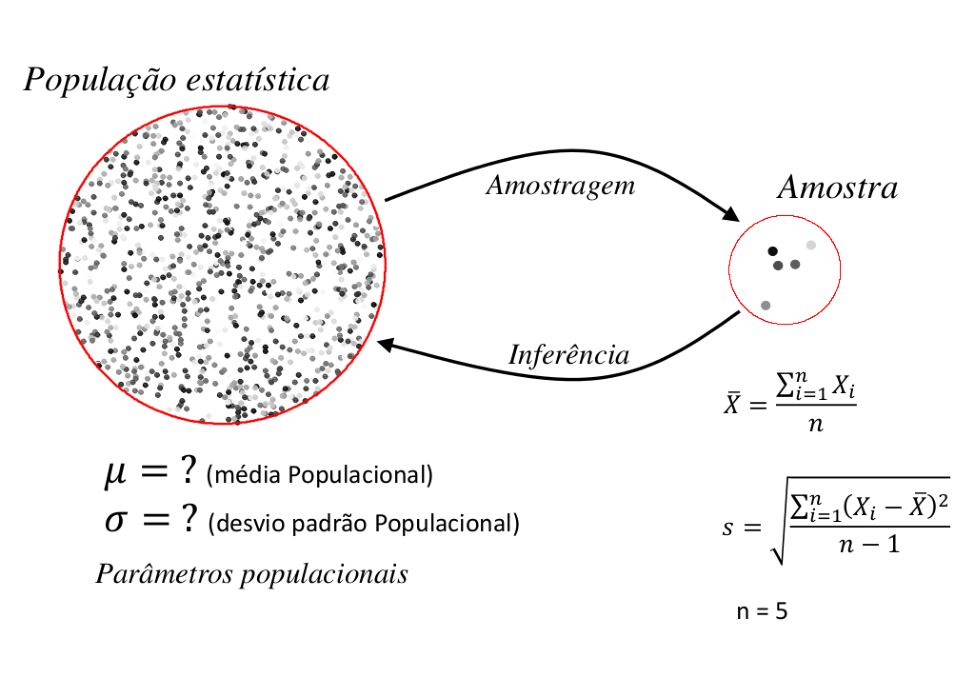
\includegraphics{probest-cambientais_files/figure-latex/amostr-1} 

}

\caption{Processo de amostragem e inferência estatística}\label{fig:amostr}
\end{figure}

\hypertarget{medidas-de-tenduxeancia-central}{%
\section{Medidas de tendência central}\label{medidas-de-tenduxeancia-central}}

Uma distribuição de frequência pode ser descrita a partir de uma \textbf{medida de tendência central} que indica o valor ao redor dos quais a maior parte das observações está concentrada. Iremos apresentar quatro destas medidas: a \textbf{média aritmética}, a \textbf{mediana}, a \textbf{moda} e o \textbf{ponto médio}.

A média aritmética é a medida de tendência central mais comum. Para uma população estatística de tamanho \textbf{N}, com \(X_1\), \(X_2\), \(X_3\), \(\cdots, X_N\) elementos, ela é referida como a \textbf{média populacional}, indicada pela letra grega \(\mu\), onde:

\[\mu=\frac{X_1+X_2+X_3+\cdots+X_N}{N}=\frac{\sum_{i=1}^N{X_i}}{N}\]

Quando nos referimos a uma amostra com \textbf{n} elementos, a média aritmética \textbf{amostral} (\(\overline{X}\)) é dada por:

\[\overline{X}=\frac{X_1+X_2+X_3+\cdots+X_n}{n}=\frac{\sum_{i=1}^n{X_i}}{n}\]

A \textbf{mediana} é outra medida de centro que pode ser definida como o valor do meio de uma distribuição, de modo que metade dos valores estão abaixo e metade está acima da mediana. A mediana, ao contrário da média, é pouco influenciada por valores extremos.

A \textbf{moda} é definida como o valor mais frequente de uma distribuição e finalmente, o \textbf{ponto médio} é calculado com base em somente dois valores da distribuição - o máximo e o mínimo, sendo obtido por:

\[P_{medio}=\frac{X_{maximo} + X_{minimo}}{2}\]

Valores extremos não têm influência sobre a moda porém têm grande efeito sobre o ponto médio.

Um conjunto de dados pode ser representado por uma distribuição de frequências e por medidas de tendencia central. Existe uma relação entre o formato de uma distribuição de frequência e a posição relativa da média aritmética, da mediana e da moda. Em um gráfico simétrico, onde as observações estão dispersas igualmente acima e abaixo do ponto central, os valores da média, mediana e moda coincidem. Este tipo de distribuição é dita \textbf{simétrica}. Por outro lado, pode ocorrer que a distribuição de valores seja \textbf{assimétrica}. Neste caso, a posição relativa da média, mediana e moda depende se a assimetria é à \textbf{direita} ou à \textbf{esquerda}. Esta discrepância ocorre devido à sensibilidade destas medidas a valores extremos na distribuição, em que a média é mais sensível que a mediana e a moda \citep{triola2017introduccao}.

\begin{figure}

{\centering 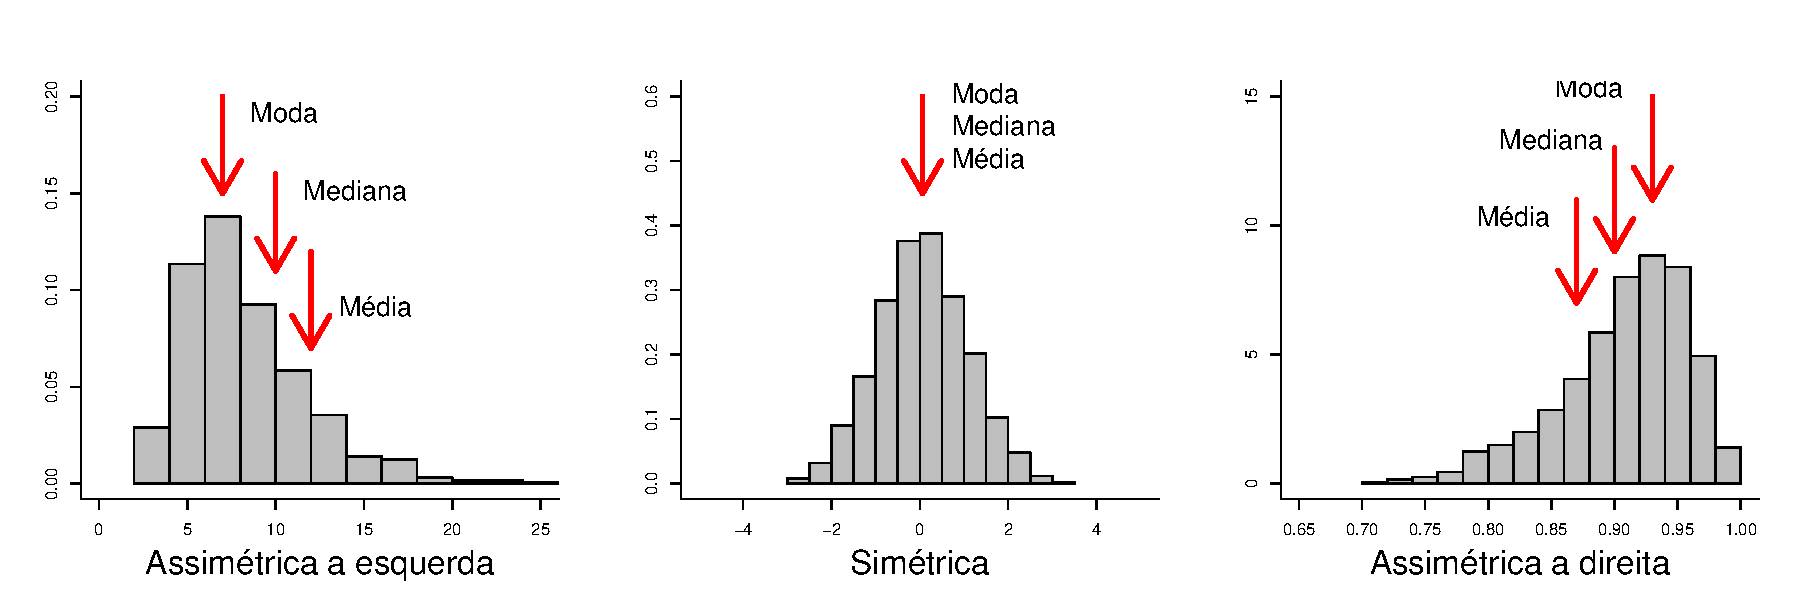
\includegraphics{probest-cambientais_files/figure-latex/assimetr-1} 

}

\caption{Efeito da assimetria de uma distribuição sobre a média aritmética, a mediana e a moda}\label{fig:assimetr}
\end{figure}

\begin{quote}
\textbf{Média}: utiliza todo o conjunto de dados. Sensível a valores extremos. Dentre todos os estimadores de tendência central é o menos variável;
\end{quote}

\begin{quote}
\textbf{Mediana}: o valor do meio. Metade dos pontos está acima e metade abaixo da mediana. A mediana é uma medida \emph{resistente} a valores extremos;
\end{quote}

\begin{quote}
\textbf{Moda}: valor mais frequente. Se mais de um valor tem a mesma frequência, os dados têm uma distribuição \emph{multimodal};
\end{quote}

\begin{quote}
\textbf{Ponto médio}: considera somente os valores máximos e mínimos. O ponto médio é fácil de calcular porém não utiliza a maioria do conjunto de dados e é \emph{muito sensível a valores extremos}.
\end{quote}

\hypertarget{medidas-de-variauxe7uxe3o}{%
\section{Medidas de variação}\label{medidas-de-variauxe7uxe3o}}

Diferente das medidas de tendência central, as \textbf{medidas de variação} indicam o grau de dispersão das observações. Distribuições com observações muito próximas à média têm \emph{baixo grau de dispersão}, enquanto aquelas com observações muito distantes da média têm \emph{alto grau de dispersão}. Vamos apresentar quatro índices que medem o grau de dispersão: a \textbf{variância}, o \textbf{desvio padrão}, o \textbf{coeficiente de variação} e a \textbf{amplitude de variação}.

A variância mede quão distante os valores estão da média aritmética. A \textbf{variância populacional} é indicada pela letra grega \(\sigma^2\), onde:

\[\sigma^2=\frac{\sum_{i=1}^N{(X_i - \mu)^2}}{N}\]

Quando nos referimos a uma amostra, a \textbf{variância amostral} é indicada por \(s^2\) e dada por:

\[s^2=\frac{\sum_{i=1}^N{(X_i - \overline{X})^2}}{n-1}\]

Note que para a variância amostral, utilizamos \(\overline{X}\) e não \(\mu\), porque estamos medindo a dispersão das observações ao redor da média \textbf{amostral}. O denominador da equação também muda para \emph{n-1} pois agora estamos nos referindo à uma amostra com \textbf{n} elementos. A subtração por \emph{n-1} é necessária para que \(s^2\) seja um estimador \textbf{não viciado} de \(\sigma^2\).

Outra medida de dispersão é o \textbf{desvio padrão} que é simplesmente a raiz quadrada da variância e portanto, dado na mesma escala de mensuração das observações originais. O desvio padrão populacional (\(\sigma\)) é dado por:

\[\sigma=\sqrt{\frac{\sum_{i=1}^N{(X_i - \mu)^2}}{N}}\]

enquanto para a amostra (\(s\)) é:

\[s=\sqrt{\frac{\sum_{i=1}^N{(X_i - \overline{X})^2}}{n-1}}\]

O \textbf{coeficiente de variação} (cv) relaciona o desvio padrão à média, sendo definido por:

\[cv = s/\overline{X}\] ou \[cv_{\%}  = s/\overline{X}\cdot 100\]

O coeficiente de variação amostral descrito acima, é um estimador do coeficiente de variação da população, onde \(s\) é substituído por \(\sigma\), e \(\overline{X}\) por \(\mu\).

Finalmente, a \textbf{amplitude de variação} é a diferença entre os pontos máximo e mínimo de um grupo de observações

Amplitude de variação = \(X_{maximo} - X_{minimo}\)

\hypertarget{exempificando-os-cuxe1lculos}{%
\subsection{Exempificando os cálculos}\label{exempificando-os-cuxe1lculos}}

Considere uma amostra do comprimento da carapaça de 10 caranguejos \(\textit{Menipe nodifrons}\):

\(X_i\) (em centímetros): 4.0, 4.1, 4.5, 4.9, 5.0, 5.0, 6.6, 7.0, 7.7, 7.9

\hypertarget{muxe9dia}{%
\subsubsection{Média}\label{muxe9dia}}

\(\overline{X}=\frac{4.0+4.1+4.5+4.9+5.0+5.0+6.6+7.0+7.7+7.9}{10}=56.7/10=5.67\)

\hypertarget{mediana}{%
\subsubsection{Mediana}\label{mediana}}

4.0, 4.1, 4.5, 4.9, \textbf{5.0, 5.0}, 6.6, 7.0, 7.7, 7.9

Mediana = \(\frac{5 + 5}{2} = 5\)

\hypertarget{moda}{%
\subsubsection{Moda}\label{moda}}

Moda = 5 (o único número que se repete mais de uma vez na distribuição)

\hypertarget{ponto-muxe9dio}{%
\subsubsection{Ponto médio}\label{ponto-muxe9dio}}

\(P_{medio}=\frac{7.9 + 4.0}{2} = 5.95\)

\hypertarget{variuxe2ncia}{%
\subsubsection{Variância}\label{variuxe2ncia}}

\(s^2=\frac{(4.0-5.67+4.1-5.67+4.5-5.67+4.9-5.67+5.0-5.67+5.0-5.67+6.6-5.67+7.0-5.67+7.7-5.67+7.9-5.67)^2}{10-1}\)

\(s^2 = 19.84/9 = 2.20\)

\hypertarget{desvio-padruxe3o}{%
\subsubsection{Desvio padrão}\label{desvio-padruxe3o}}

\(s=\sqrt{2.20} = 1.48\)

\hypertarget{coeficiente-de-variauxe7uxe3o}{%
\subsubsection{Coeficiente de variação}\label{coeficiente-de-variauxe7uxe3o}}

\(cv = 1.48/5.95 \cdot 100 = 26.19\%\)

\hypertarget{medidas-de-posiuxe7uxe3o}{%
\section{Medidas de posição}\label{medidas-de-posiuxe7uxe3o}}

A média, mediana, moda e ponto médio são um tipo de \textbf{medidas de posição} que indicam uma posição particular, a posição central ao redor da qual os dados estão dispersos. Existem outras medidas de posição que indicam posições particulares. Vamos abordar aqui as posições dos \textbf{quartis} e o \textbf{índice Z}. Estas são as medidas mais utilizadas em análise e interpretação de dados.

\hypertarget{quartis}{%
\subsection{Quartis}\label{quartis}}

Os quartis de uma distribuição de valores são obtidos após ordenarmos os dados em ordem crescente e em seguida dividí-los dados em partes iguais, contendo cada uma 25\% do número total de observações. Se temos 20 observações, cada parte conterá portanto cinco observações, \(20 \times 0.25 = 5\) e os quartis são as posições que dividem estas partes.

Os quartis podem ser indicados por \(Q_1\), \(Q_2\) e \(Q_3\), conforme a figura abaixo.

\begin{figure}

{\centering 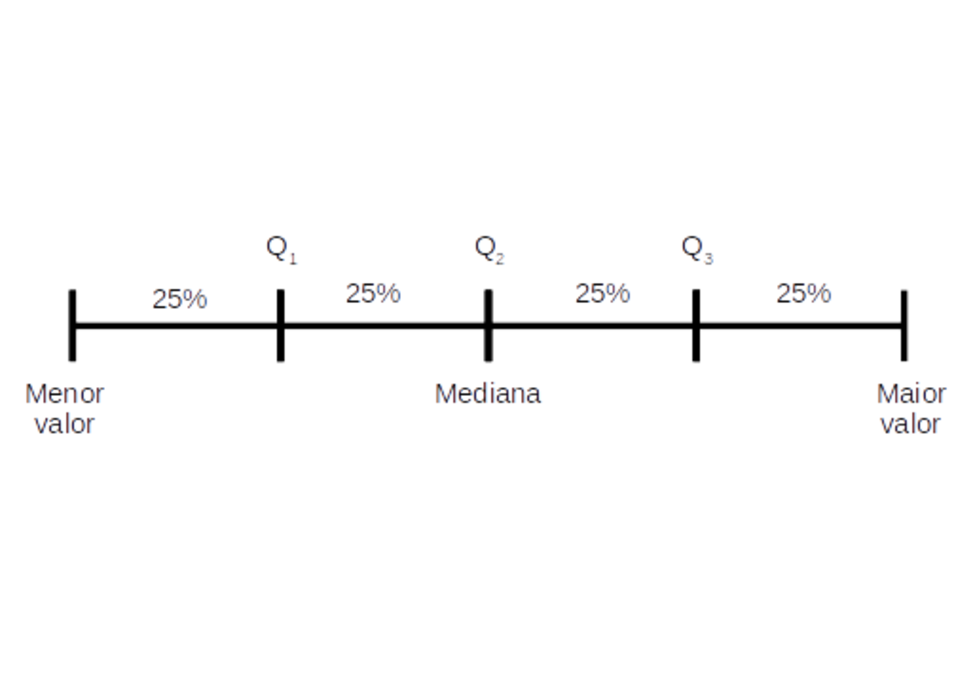
\includegraphics{probest-cambientais_files/figure-latex/quartisfig-1} 

}

\caption{Divisão de uma distribuição de valores em quartis}\label{fig:quartisfig}
\end{figure}

\begin{quote}
\(Q_{1}\) O ponto que separa os 25\% \textbf{menores} valores do restante da distribuição.
\end{quote}

\begin{quote}
\(Q_{2}\): O ponto que separa os 50\% \textbf{menores} valores dos 50\% \textbf{maiores}. Este coincide com a Mediana apresentada anteriormente.
\end{quote}

\begin{quote}
\(Q_{3}\): O ponto que separa os 25\% \textbf{maiores} valores do restante da distribuição.
\end{quote}

\hypertarget{cuxe1lculo-dos-quartil-na-posiuxe7uxe3o-j-q_j}{%
\subsubsection{\texorpdfstring{Cálculo dos quartil na posição \(j\) (\(Q_j\))}{Cálculo dos quartil na posição j (Q\_j)}}\label{cuxe1lculo-dos-quartil-na-posiuxe7uxe3o-j-q_j}}

\begin{enumerate}
\def\labelenumi{\arabic{enumi}.}
\item
  Seja \(n\) o número de observações em \(X\), arrange a variável \(X\) em ordem crescente. Deste modo \(X_1\) será o menor valor e \(X_n\) o maior valor. Iremos expressar um valor particular na distribuição de X em ordem crescente como \(X_k\);
\item
  Calcule \(L = \frac{j \times (n+1)}{4}\);
\item
  Defina \(k\) como o maior número inteiro abaixo de \(L\);
\item
  Calcule \(Q_j = X_k + (L - k) \times (X_{k+1}-X_k)\);
\end{enumerate}

\(Q_j\) será um elemento entre \(X_k\) e \(X_{k+1}\) e se \(X_k\) for um número inteiro, \(Q_j = X_k\)

\hypertarget{exemplo-para-o-cuxe1lculo-de-q_1}{%
\paragraph{\texorpdfstring{Exemplo para o cálculo de \(Q_1\)}{Exemplo para o cálculo de Q\_1}}\label{exemplo-para-o-cuxe1lculo-de-q_1}}

Considere a variável \(X\) com \(n =\) 20 observações.

\(X\) = 8.7, 10.4, 8.3, 13.2, 10.7, 8.4, 11, 11.5, 11.2, 9.4, 13, 10.8, 8.8, 5.6, 12.2, 9.9, 10, 11.9, 11.6, 11.2

\begin{tabular}{l|r}
\hline
Posicao k & X ordenado\\
\hline
1a Posição & 5.6\\
\hline
2a Posição & 8.3\\
\hline
3a Posição & 8.4\\
\hline
4a Posição & 8.7\\
\hline
5a Posição & 8.8\\
\hline
6a Posição & 9.4\\
\hline
7a Posição & 9.9\\
\hline
8a Posição & 10.0\\
\hline
9a Posição & 10.4\\
\hline
10a Posição & 10.7\\
\hline
11a Posição & 10.8\\
\hline
12a Posição & 11.0\\
\hline
13a Posição & 11.2\\
\hline
14a Posição & 11.2\\
\hline
15a Posição & 11.5\\
\hline
16a Posição & 11.6\\
\hline
17a Posição & 11.9\\
\hline
18a Posição & 12.2\\
\hline
19a Posição & 13.0\\
\hline
20a Posição & 13.2\\
\hline
\end{tabular}

\begin{enumerate}
\def\labelenumi{\arabic{enumi}.}
\item
  Arrange \(X\) em ordem crescente
\item
  Calcule \(L = \frac{1 \times (20+1)}{4} = 5.25\);
\item
  Defina \(k\) como o maior número inteiro abaixo de \(L\). Portanto, \(k = 5\). Veja que a observação correspondente à 5\(^a\) posição é 8.8 e a 6\(^a\) posição 9.4.
\item
  Calcule \(Q_1 = 8.8 + (5.25 - 5) \times (9.4-8.8) = 8.95\);
\end{enumerate}

\textbf{Observação}: Calcule \(Q_2\) e \(Q_3\) e verifique se os resultados são: \(Q_2 = 10.75\) e \(Q_3 = 11.575\)

\hypertarget{representando-quartis-em-boxplots}{%
\subsubsection{Representando quartis em Boxplots}\label{representando-quartis-em-boxplots}}

Os quartis de uma distribuição no ajudam a entender o formato de uma distribuição. Uma das formas amplamemte estabelecidas de representarmos graficamente os quartis são por meio de um gráfico denominado de \textbf{Boxplot}. Para a variável acima o boxplot será:

\begin{figure}

{\centering 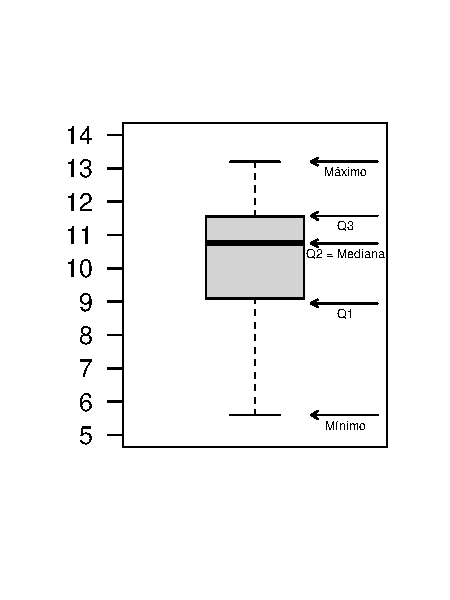
\includegraphics{probest-cambientais_files/figure-latex/boxquartis-1} 

}

\caption{Divisão em quartis de um boxplot}\label{fig:boxquartis}
\end{figure}

Em um boxplot, a linha central mais expessa representa a \textbf{Mediana} ou \(2^o\) quartil, os limites da caixa são o \(1^o\) e \(3^o\) quartis e as extremidades geralmente são os pontos máximo e mínimo da dsitribuição.

Existe uma relação entre os \textbf{histogramas} e os \textbf{boxplots}. Ambos podem ser utilizados para avaliarmos o grau de \textbf{assimetria} de uma distribuição como pode ser visto abaixo. Em uma distribuição simétrica, a caixa do boxplot tende a se concentrar no meio da distribuição, enquanto que em distribuições assimétricas, a caixa tende a ficar deslocada à esquerda o à direita.

\begin{figure}

{\centering 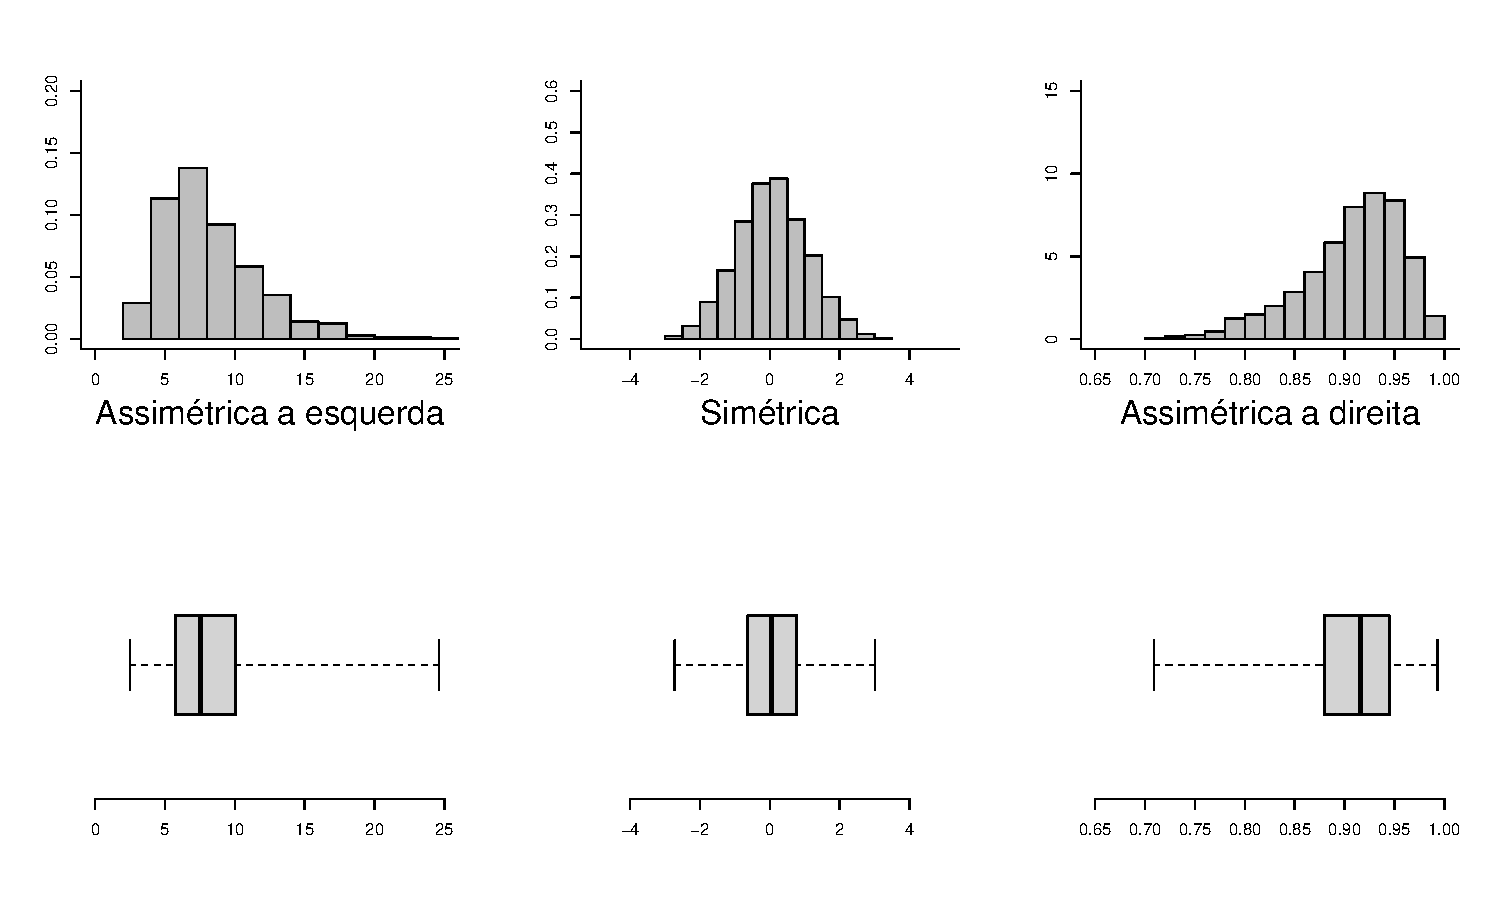
\includegraphics{probest-cambientais_files/figure-latex/histbox-1} 

}

\caption{Relação entre as representações por meio de histogramas e boxplots}\label{fig:histbox}
\end{figure}

\hypertarget{uxedndice-z}{%
\subsection{Índice Z}\label{uxedndice-z}}

O \textbf{Índice Z} ou \textbf{Escore Z} indica a posição de uma observação particular (\(X_i\)). O valor de \(Z\) relaciona a posição de \(X_i\) com a \textbf{média} e o \textbf{desvio padrão} da distribuição. Suponha uma população com distribuição normal com média \(\mu\) e desvio padrão \(\sigma\). O índice de \(Z_i\) para uma obserrvação particular é calculado por:

\[Z_i = \frac{X_i - \mu}{\sigma}\]

Se o índice Z é calculado para uma amostra da população com média \(\bar{X}\) e desvio padrão \(s\), seu calculo se dá por:

\[Z_i = \frac{X_i - \bar{X}}{s}\]

\hypertarget{exemplo}{%
\subsubsection{Exemplo}\label{exemplo}}

Retornemos à variável X descrita acima:

\(X\) = 8.7, 10.4, 8.3, 13.2, 10.7, 8.4, 11, 11.5, 11.2, 9.4, 13, 10.8, 8.8, 5.6, 12.2, 9.9, 10, 11.9, 11.6, 11.2

A média e o desvio padrão de X são respectivamente \(\bar{X} = 10.39\) e \(s = 1.82\).

Vamos calcular o índice Z para a observação \(X = 8.3\)

\(Z = \frac{8.3 - 10.39}{1.82} = -1.15\)

Veja que o score Z é negativo e portanto, \(X_i\) está abaixo da média.

\hypertarget{interpretando-o-valor-de-z}{%
\subsubsection{Interpretando o valor de Z}\label{interpretando-o-valor-de-z}}

O valor de Z indica quantos desvio padrões uma determinada observação está acima ou abaixo da média do grupo de observações. Os resultados de Z podem ser:

\begin{itemize}
\tightlist
\item
  \(Z = 0\): \(X_i = \bar{X}\);
\item
  \(Z > 0\): \(X_i > \bar{X}\);
\item
  \(Z < 0\): \(X_i < \bar{X}\);
\end{itemize}

Para uma distribuição com média igual 10 e desvio padrão igual a 2, uma observação X = 14 está dois desvios padrões acima da sua respectiva média. Neste caso, Z valeria 2 como pode ser verificado na equação abaixo

\[Z = \frac{14 - 10}{2} = 2\]

Vamos calcular os valores de Z para a variável X acima e analisar os resultados

\begin{tabular}{l|r|r}
\hline
Posicao k & X ordenado & Z ordenado\\
\hline
1a Posição & 5.6 & -2.63\\
\hline
2a Posição & 8.3 & -1.15\\
\hline
3a Posição & 8.4 & -1.09\\
\hline
4a Posição & 8.7 & -0.93\\
\hline
5a Posição & 8.8 & -0.87\\
\hline
6a Posição & 9.4 & -0.54\\
\hline
7a Posição & 9.9 & -0.27\\
\hline
8a Posição & 10.0 & -0.21\\
\hline
9a Posição & 10.4 & 0.01\\
\hline
10a Posição & 10.7 & 0.17\\
\hline
11a Posição & 10.8 & 0.23\\
\hline
12a Posição & 11.0 & 0.34\\
\hline
13a Posição & 11.2 & 0.45\\
\hline
14a Posição & 11.2 & 0.45\\
\hline
15a Posição & 11.5 & 0.61\\
\hline
16a Posição & 11.6 & 0.66\\
\hline
17a Posição & 11.9 & 0.83\\
\hline
18a Posição & 12.2 & 0.99\\
\hline
19a Posição & 13.0 & 1.43\\
\hline
20a Posição & 13.2 & 1.54\\
\hline
\end{tabular}

\begin{center}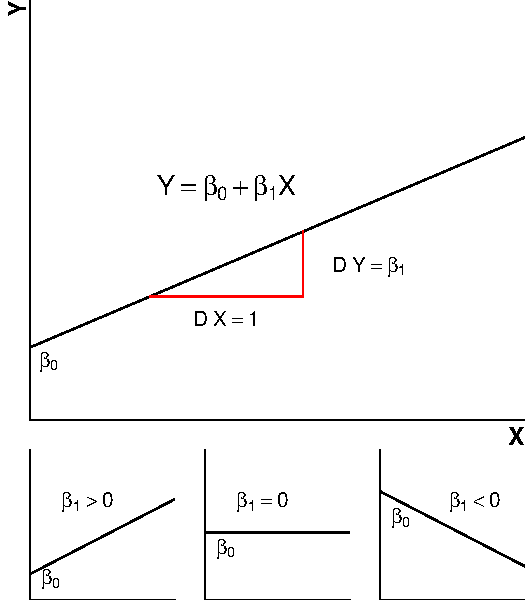
\includegraphics{probest-cambientais_files/figure-latex/unnamed-chunk-43-1} \end{center}

Veja na tabela que conforme o valor de \(X_i\) se distancia da média de \(X = 10.39\) mais distante de zero será o valor Z. Neste exemplo, as observações mais extremas de X estão, respectivamente, a -2.63 desvios padrões abaixo e 1.54 desvios padrões acima da média.

\hypertarget{valores-esperados-de-z-em-uma-distribuiuxe7uxe3o-normal-padronizada}{%
\subsubsection{Valores esperados de Z em uma distribuição normal padronizada}\label{valores-esperados-de-z-em-uma-distribuiuxe7uxe3o-normal-padronizada}}

A interpretação de Z faz sentido quando desejamos comparar uma determinada observação \(X_i\) à posição que esta teria dentro de uma \textbf{Distribuição Normal Padronizada} (Capítulo \ref{normtlc}). A figura abaixo nos permite avaliar qual a probabilidade de encontrarmos uma observação a diferentes distâncias da média populacional. Suponha que tomemos uma amostra de uma distribuição normal. Existe uma probabilidade de aproximadamente 68\% de que esta amostra esteja 1 desvio padrão acima ou abaixo da média. Esta probabilidade aumenta para cerca de 95\% se considerarmos uma distância dois desvios padrões acima ou abaixo da média. Por outro lado, que é muito \textbf{improvável} amostrarmos um valor a mais de 3 desvios padrões da média. Isto rá ocorrer em somente de 0.2\% dos casos.

\begin{center}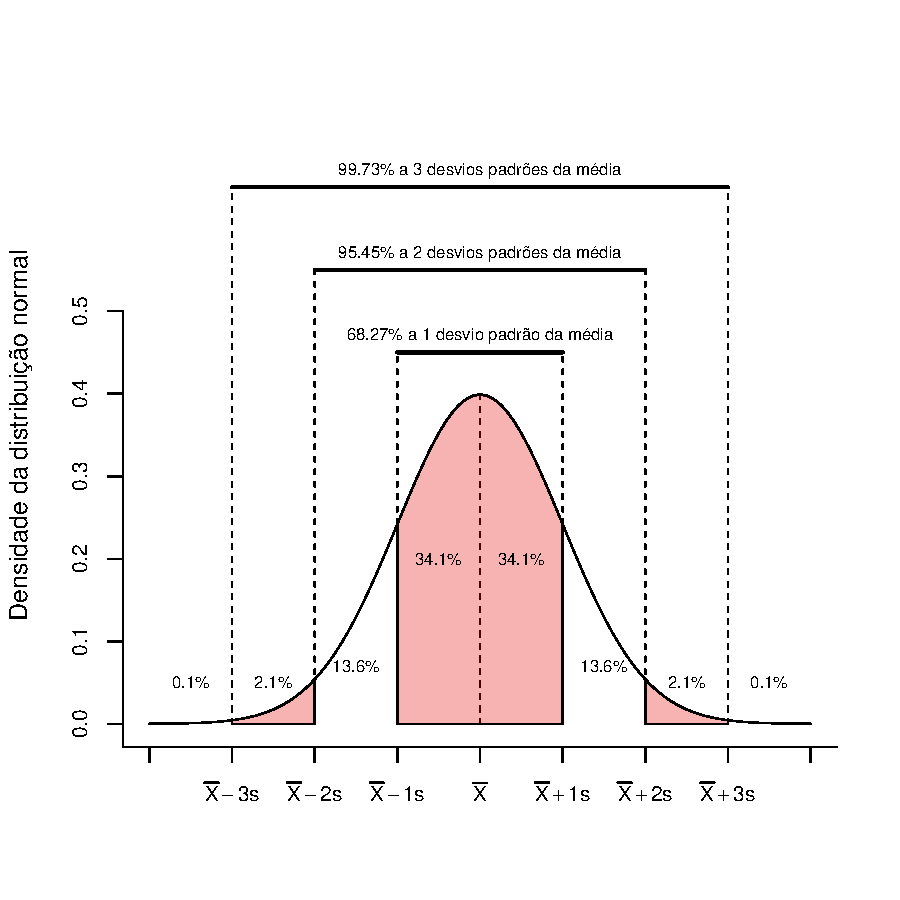
\includegraphics{probest-cambientais_files/figure-latex/distrnorm-1} \end{center}

Este assunto será abordado em mais detalhes no tópico de inferêcnia estatística. No entanto, suponha por exemplo que a distribuição de altura de homens adultos siga uma distribuiçao normal com média \(\mu = 175\) cm e desvio padrão de \(\sigma = 20\) cm. Segundo a expectativa teórica portanto, menor de 5\% dos homens adultos têm \(\mu \pm 2 \times \sigma = 175 \pm 2 \times 20 = 175 \pm 40\). Ou seja, menos de 5\% dos homens têm mais de 215 cm ou menos de 135 cm de altura.

\hypertarget{volume-dos-reservatuxf3rios-da-grande-suxe3o-paulo-visualizando-medidas-de-posiuxe7uxe3o-e-variauxe7uxe3o}{%
\section{Volume dos reservatórios da Grande São Paulo: visualizando medidas de posição e variação}\label{volume-dos-reservatuxf3rios-da-grande-suxe3o-paulo-visualizando-medidas-de-posiuxe7uxe3o-e-variauxe7uxe3o}}

Vamos retornar aos dados sobre volume dos sistemas de abastecimento de água da Gande São Paulo (Capítulo \ref{descrit}) e extrair a média, desvio padrão e quantis para cada sistema.

\begin{tabular}{l|r|r|r|r|r}
\hline
Sistema & Média & Desvio padrão & Q1 & Q2 & Q3\\
\hline
AltoTiete & 48.62 & 16.08 & 38.8575 & 51.495 & 57.8175\\
\hline
Cantareira & 48.91 & 23.66 & 35.1350 & 48.555 & 60.2800\\
\hline
Cotia & 78.04 & 22.28 & 71.3550 & 85.300 & 93.6450\\
\hline
Guarapiranga & 68.43 & 13.11 & 61.6175 & 72.075 & 75.2175\\
\hline
RioClaro & 82.27 & 15.94 & 75.3100 & 87.025 & 93.1375\\
\hline
RioGrande & 87.06 & 5.13 & 84.2825 & 87.595 & 90.5875\\
\hline
\end{tabular}

Os Sistemas Alto Tietê e Cantareira têm, aparentemente, os menores volumes médios emquanto os Sistemas Rio Claro e Rio Grande, mantêm os maiores volumes. Veja também que o volume médio anual no Sistema Rio Grande manteve-se altamente constante ao longo dos anos, apresentando um desvio padrão de 5.13, contra valores próximos a 15 ou 20 nos demais Sistemas. Compare estes resultados com os gráficos de linha que fizemos anteriormente e com os boxplots a seguir.

\begin{center}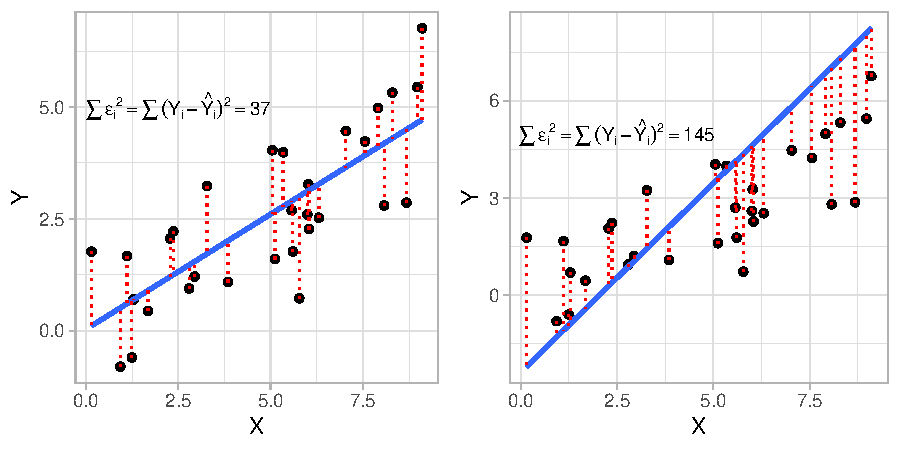
\includegraphics{probest-cambientais_files/figure-latex/unnamed-chunk-46-1} \end{center}

Veja que novamente, os Sistemas Alto Tietê e Cantareira aparecem com menores volumes e contrastam com os demais. Os regimes de chuva são semelhantes, exceto para o Sistema Rio Claro no município de Salesópolis, com pluviosidade geralmente mais elevada.

\hypertarget{part-amostragem-e-inferuxeancia-estatuxedstica}{%
\part{Amostragem e Inferência Estatística}\label{part-amostragem-e-inferuxeancia-estatuxedstica}}

\hypertarget{amostrmedias}{%
\chapter{Amostrando uma População Estatística}\label{amostrmedias}}

O objetivo da amostragem é descrever características da \textbf{população estatística} por meio de características da \textbf{amostra}. E um estudo sobre o diâmetro dos caules de \emph{Rhizophora mangle} em um manguezal (DAP: diâmetro a altura do peito), a população estatística são os diâmetros de todas as árvores do referido manguezal. A população estatística pode ser descrita por \textbf{parâmetros} que representam medidas de centro como o diâmetro médio (\(\mu\)), ou por medidas de variação como o desvio padrão (\(\sigma\)), que representam o grau de dispersão das unidades amostrais ao redor da média. Se amostramos \textbf{n} elementos desta população, a média amostral (\(\overline{X}\)) e o desvio padrão amostral (\(s\)) dos diâmetros serão os estimadores destas características.

Dependendo da questão envolvida e do conhecimento prévio sobre a população, diferentes métodos de amostragem são apropriados. A \textbf{teoria da amostragem} é a área da ciência que estuda estes métodos. Neste capítulo vamos discutir três tipos de amostragem: \textbf{aleatória simples}, \textbf{estratificada} e \textbf{sistemática}.

\hypertarget{amostragem-aleatuxf3ria-simples}{%
\section{Amostragem aleatória simples}\label{amostragem-aleatuxf3ria-simples}}

É aquela em que cada elemento da população tem a mesma probabilidade de ser selecionado para compor a amostra. Por exemplo, se a população consiste de 1000 elementos, cada um terá uma probabilidade de \(\frac{1}{1000}\) de ser escolhido. Isto isenta o pesquisador de tomar qualquer decisão com base em julgamentos pré-concebidos, sobre quais alementos devem ou não compor a amostra.

Para exemplificar suponha uma população hipotética de somente 10 elementos:

\textbf{População}: 3, 10, 14, 19, 27, 28, 29, 41, 42, 43

Em uma amostra aleatória simples de cinco elementos, qualquer combinação destes 10 elementos é \textbf{igualmente provável}. Se por puro acaso sortearmos uma amostra aleatória contendo os cinco menores valores da população:

\textbf{Amostra 1}: 3, 10, 14, 19, 27

A amostra seria \textbf{tão aleatória} é válida do ponto de vista amostral quanto qualquer outra como:

\textbf{Amostra 2}: 27, 28, 42, 3, 43

Isto significa que uma amostra aleatória pode não ser \textbf{necessariamente} representativa da população. Amostras pequenas por exemplo, têm uma chance maior de selecionar apenas valores extremos, ou seja, os maiores ou menores elementos da população. A média amostral (\(\bar{X}\)) calculada para estas amostras estará distante da média populacional (\(\mu\)).
No entanto, a importância central da amostragem aleatória em estatística está no fato de que a aleatoriedade produz, \textbf{em média}, amostras representativas da população. Deste modo, é esperado que na maioria das vezes, uma amostra aleatória gere médias amostrais próximas à média populacional. Por este motivo, é fundamental prezar pela aleatoriedade no processo amostral, pois de outro modo não poderemos garantir que a inferência seja válida com base nas leis de probabilidade.

O modo mais direto de se obter uma amostra aleatória é por meio de sorteio. Após atribuir números de 1 a \(N\) a cada unidade amostral, estas unidades são sorteadas até que seja atingido o tamanho \(n\) desejado. Na prática, nem sempre é possível obtermos uma amostra aleatória nestes moldes. Para o exemplo do DAP de \emph{Rhizophora mangle}, não seria viável primeiramente enumerar todas as árvores para, após um sorteio, tomar as medidas somente das árvores que foram selecionadas. Entretanto, se tivermos as coordenadas geográficas da área, poderíamos sortear \(n\) posições no espaço e, chegando ao local desejado, escolher a árvore mais próxima da coordenada sorteada. Este procedimento nos daria um resultado igualmente válido, no sentido de garantir uma escolha aleatória das unidades amostrais. Outras dificuldades práticas obviamente seriam possíveis neste procedimento, como garantir acesso irrestrito à toda a área ou tempo disponível para percorrer a toda região. Questões como estas não desmerecem o requisito básico de se obter uma amostra aleatória, mas nos auxiliam a decidir como conciliar a prática experimental com a necessidade da aleatorização em um experimento.

\hypertarget{amostragem-aleatuxf3ria-estratificada}{%
\section{Amostragem aleatória estratificada}\label{amostragem-aleatuxf3ria-estratificada}}

Se tivermos algum conhecimento prévio de como a população está estruturada, a amostra aleatória simples, embora não esteja incorreta, pode não ser a estratégia mais eficiente. Se for possivel identificar \textbf{estratos} ou \textbf{subgrupos} dentro da população, podemos conduzir uma \textbf{amostragem aleatória estatificada}.

Voltemos ao exemplo da \emph{Rhizophora mangle}. Suponha que o manguezal em estudo possa ser dividido em duas áreas. Uma área que foi recentemente perturbada por ações antrópicas e encontra-se em estado de regeneração, e uma área que sempre esteve livre da ação humana. Espera-se que as árvores na área íntegra sejam mais velhas e portanto tenham em média DAPs maiores, enquanto na área em regeneração os DAPs médios sejam menores.

Em uma amostra aleatória simples, sobretudo se for pequena, é possível que puramente ao acaso, um ou outro estrato se torne mais representado. Isto tornará as estimativas mais variáveis. Se dermos azar da maioria das unidades amostrais serem sorteadas do estrato íntegro, teremos estimativas de DAP muito acima de \(\mu\). No entanto, se a seleção dos indivíduos foi feita por meio de sorteio, o simples fato de observarmos este padrão não é por si só justificativa para refarzermos a amostra. O ponto relevante aqui é que em uma amostra aleatória simples estes extremos indesejáveis são mais prováveis de acontecer.

Em uma amostragem estratificada o esforço amostral é subdividito entre os estratos, que em nosso exemplo seriam as áreas integra e perturbada. O tamanho amostral em cada estrato será o mesmo, ou \textbf{proporcional} ao tamanho do estrato. Após definirmos o tamanho amostral em cada estrato, as unidades amostrais são selecionadas por meio de uma amostragem aleatória simples. Deste modo, teremos certeza de que \textbf{todos} os estratos estarão representados na amostra conforme sua representatividade na população e as estimativas tenderão a se concentrar mais próximas à \(\mu\) se compararmos com os resultados de uma amostra aleatória simples.

Quando os estratos são identificados \textbf{corretamente}, a principal vantagem da amostra aleatória estratificada sobre a amostra aleatória simples está em aumentar a \textbf{precisão} das estimativas. Mais a frente iremos discutir os conceitos de precisão e acurácia e relacioná-los com as estratégias amostrais discutidas aqui.

\hypertarget{amostragem-sistemuxe1tica}{%
\section{Amostragem sistemática}\label{amostragem-sistemuxe1tica}}

Uma amostragem sistemática é possível quando as unidades amostrais podem ser ordenadas. A ordenação segue alguma característica da unidade como peso, idade, salinidade, posição no espaço ou intervalo de tempo. O objetivo é garantir que a amostra inclua todo o intervalo de variação da população. Neste tipo de amostragem, selecionamos um elemento inicial e, em intervalos regulares, selecionamos os demais elementos.

Em nossa amostragem de \emph{Rhizophora mangle}, poderíamos ordenar as árvores da menor para a maior, selecionar uma árvore inicial (p.~ex. a \(5^a\)) e um intervalo (por exemplo a cada 10 árvores). A amostragem iria consistir da \(5^a\), \(15^a\), \(25^a\), \(35^a\), \(\cdots\) árvores, até chegarmos ao maior indivíduo. Deste modo, saberíamos que todo o intervalo de DAPs estaria representado na amostra. Obviamente este exemplo é inviável, pois necessitaríamos de uma lista de \textbf{prévia} do tamanho e posição de todas as árvores antes de conduzirmos a amostragem. Um exemplo de amostragem sistemática mais factível, seria definir alguns transectos lineares e dispor \(n\) pontos equidistantes. A amostra iria consistir dos DAPs mensurados nas árvores imediatamente mais próximas a cada um dos pontos. Se o comprimento e direção dos transectos forem bem escolhidos, garantimos que toda a área de estudo seja abrangida. Neste caso, o protocolo de amostragem não visou exatamente atingir todos os comprimentos, mas permitir um acesso mais homogêneo a toda a àrea de distribuição dos indivíduos, \textbf{assumindo} que de alguma forma, isto também nos permita acessar toda a variação de tamanho dos indivíduos presentes na região.

\begin{figure}

{\centering 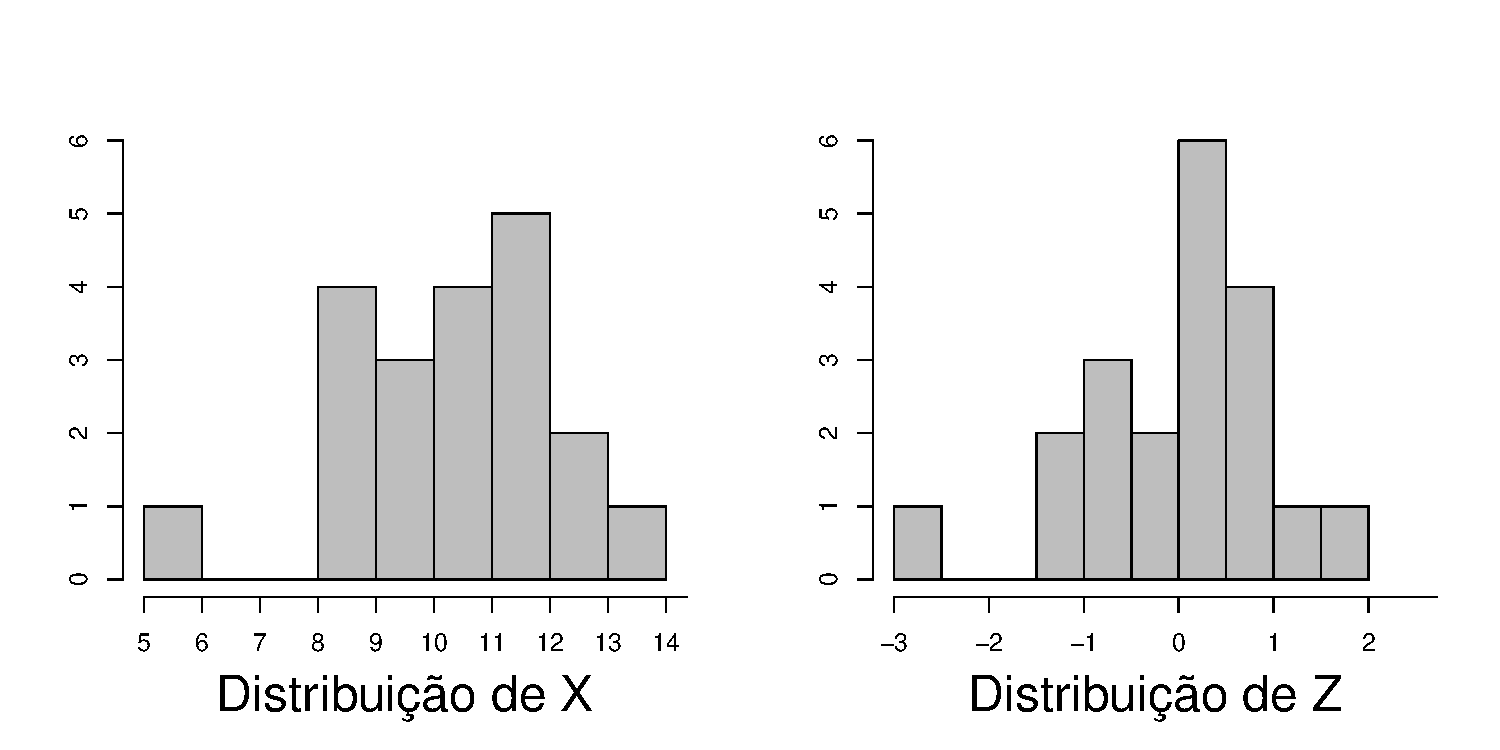
\includegraphics{probest-cambientais_files/figure-latex/unnamed-chunk-50-1} 

}

\caption{Representação de uma área com árvores de tamanhos médios agregados. (B): Em uma amostragem aleatória de com n pequeno, corremos maior risco de termos uma distribuição não representativa das unidades amostrais. (C): A amostragem estratificada resolve este problema uma vez que pois todos os blocos ou estratos serão necessariamente representados na amostra. (C): Uma vez bem definida, a amostragem ssitematica também possibilita a representatividade das unidades amostrais ao longo de todo o intervalo de variação.}\label{fig:unnamed-chunk-50}
\end{figure}

A escolha da amostragem sistemática ao invés de uma amostragem aleatória simples, se deve à sua praticidade. Se a característica de interesse das unidades amostrais estiver disposta de forma aleatória ao longo do transecto escolhido, os dois métodos irão gerar resultados similares. Na maioria dos casos, é isto que o pesquisador assume (ainda que implicitamente) quando opta por uma amostragem sistemática. Por outro lado, se houver um gradiente justamente na direção do transecto, a variância amostral irá \textbf{superestimar} a variância populacional equanto, se houver uma periodicidade que coincida com o intervalo escolhido, a variância amostral irá \textbf{subestimar} a variância populacional.

\hypertarget{erro-amostral-acuruxe1cia-e-precisuxe3o}{%
\section{Erro amostral, acurácia e precisão}\label{erro-amostral-acuruxe1cia-e-precisuxe3o}}

Como as estimativas são obtidas de um subconjunto da população (a amostra), é regra que o resultado obtido de uma amostra aleatória particular, não será igual ao verdadeiro valor da população (o parâmetro), embora exista uma grande probabilidade estar próximo. O \textbf{erro amostral} é a diferença entre uma estimativa em particular e a média populacional e portanto, é inerente à variabilidade do processo de amostragem. Suponha que, puramente ao acaso, a amostra inclua os menores elementos da população. A média amostral (\(\overline{X}\)) estará abaixo da média populacional (\(\mu\)) e o erro amostral será grande. O erro amostral é dado por \(E = \overline{X} - \mu\). A estatística estuda o comportamento probabilístico dos erros amostrais. Existe também o \textbf{erro não amostral} que decorre de equívocos de amostragem, inexperiência do amostrador, falha de equipamentos, enganos no cômputo dos resultados, etc. A estatística não é capaz de lidar com estes erros.

\textbf{Acurácia} se refere à proximidade entre o parâmetro e a estimativa \textbf{média}. Um estimativa acurada será, em média, igual ao parâmetro populacional. Diferente do erro amostral, a acurácia não se refere a uma estimativa em particular, mas ao valor \textbf{esperado} da estimativa, caso a amostragem fosse repetida um grande número de vezes.
Uma estimativa não-acurada (\textbf{viciada}) resulta em valores \textbf{consistentemente} diferentes do parâmetro, podendo estar acima (\textbf{viés positivo}) ou abaixo (\textbf{viés negativo}) do verdadeiro valor populacional. Uma estimativa viciada pode resultar de um processo amostral equivocado ou do uso de um estimador não apropriado.

\textbf{Precisão} tem relação com a variabilidade da estimativa. Estimadores que geram estimativas similares entre si são precisos. Porém, se as estimativas estiverem distantes de sua média, o estimador será pouco preciso. Já dissemos que uma amostragem aleatória estratificada, se conduzida corretamente, irá produzir estimativas mais precisas que uma amostra aleatória simples.

O objetivo da amostragem é obter estimativas precisas e acuradas. Porém, na impossibilidade de obtermos um censo, os parâmetros da população jamais serão conhecidos, de modo que é muito difícil termos uma ideia do grau de acurácia de nossas estimativas. Esta questão é conhacida como o \emph{paradoxo da amostragem}:

\begin{quote}
\emph{O paradoxo central da amostragem} é que é impossível saber, a partir da observação da amostra, se ela é ou não uma boa amostra, no sentido de que seja livre de viés \citep{stuart1984ideas}".
\end{quote}

\begin{figure}

{\centering 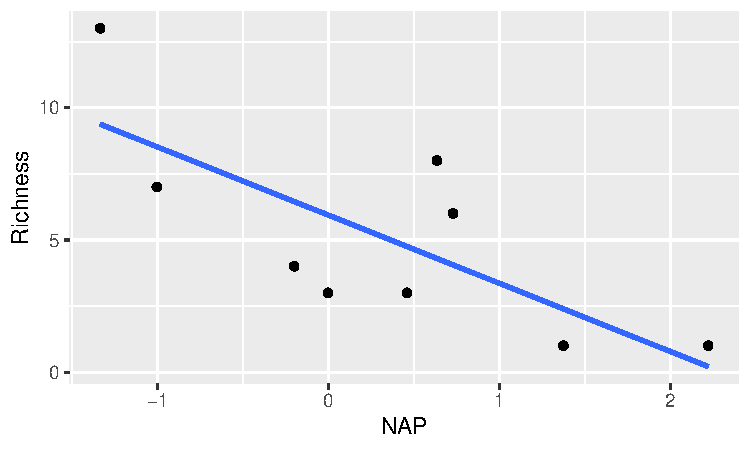
\includegraphics{probest-cambientais_files/figure-latex/unnamed-chunk-51-1} 

}

\caption{Representação dos conceitos de precisão e acurácia.}\label{fig:unnamed-chunk-51}
\end{figure}

\hypertarget{erro-amostral}{%
\subsection{Erro amostral}\label{erro-amostral}}

Voltemos à nossa população fictícia com somente 10 elementos:

\textbf{Populaçao}: 3, 10, 14, 19, 27, 28, 29, 41, 42, 43

Para esta população em particular nós conhecemos a média populacional (\(\mu\) = 25.6), de modo que será possível compará-la com as estimativas amostrais.

O que acontece se tomarmos uma amostra aleatória de tamanho \(n = 5\):

\textbf{Amostra 1}: 41, 14, 42, 29, 19

Para esta amostra, a média vale: \(\overline{X} =\frac{41+14+42+29+19}{5} = 29\).

Os valores \(\mu = 25.6\) e \(\overline{X} = 29\) não são idênticos, pois a amostra contém somente alguns elementos da população. A diferença entre \(\mu\) e \(\overline{X}\) é o chamamos de \textbf{erro amostral}.

Neste caso, o erro amostral é:

\textbf{Erro amostral 1}: \(E_1 = 29 - 25.6 = 3.4\)

Se tomarmos outra amostra aleatória, teremos outro conjunto de unidades amostrais, e consequentemente, um \(\overline{X}\) e um erro amostral diferentes. Por exemplo:

\textbf{Amostra 2}: \(27, 29, 19, 10, 14\)

\textbf{Média amostral 2}: \(\overline{X_2} = 19.8\)

\textbf{Erro amostral 2}: \(E_2 = 19.8 - 25.6 = -5.8\)

\hypertarget{acuruxe1cia}{%
\subsection{Acurácia}\label{acuruxe1cia}}

Até agora, analisamos duas amostras diferentes da população. Porém, quantas amostras distintas seriam possíveis? Para uma população com 10 elementos, a teoria combinatória nos diz que são possíveis:

\[{{10}\choose{5}} \frac{10!}{(10-5)! \times 5!} = 252\]

formas diferentes de combinarmos \(N = 10\) elementos em amostras de tamanho \(n = 5\).

Inicialmente vamos avaliar a questão com um número menor. Sejam por exemplo, 8 amostras tomadas aleatoriamente, gerando os resultados a seguir:

\begin{tabular}{l|r|r|r|r|r|r|r|r}
\hline
  & A 1 & A 2 & A 3 & A 4 & A 5 & A 6 & A 7 & A 8\\
\hline
 & 19.0 & 29 & 10.0 & 19.0 & 42.0 & 29.0 & 28 & 43.0\\
\hline
 & 29.0 & 43 & 14.0 & 41.0 & 29.0 & 10.0 & 42 & 28.0\\
\hline
 & 10.0 & 28 & 42.0 & 43.0 & 41.0 & 27.0 & 10 & 42.0\\
\hline
 & 42.0 & 3 & 28.0 & 28.0 & 14.0 & 42.0 & 43 & 27.0\\
\hline
 & 43.0 & 27 & 29.0 & 3.0 & 28.0 & 43.0 & 27 & 19.0\\
\hline
Medias & 28.6 & 26 & 24.6 & 26.8 & 30.8 & 30.2 & 30 & 31.8\\
\hline
\end{tabular}

Cada coluna desta matriz corresponde a uma possível amostra aleatória e suas respectivas médias.

Algumas amostras tiveram médias muito distantes de \(\mu\), como: \(\overline{X_{8}} = 31.8\) ou \(\overline{X_{3}} = 24.6\). Esta variação é natural do processo amostral. Os métodos de amostragem e de inferência estatística tratam justamente de como lidar e interpretar esta variação. Para entender melhor este processo, vamos obter \textbf{todas} as 252 combinações possíveis de amostras com \(n = 5\) e, em seguida, extrair suas respectivas médias.

Os resultados das 252 médias possíveis podem ser vistos a seguir, ordenados da menor para a maior média possível:

\begin{tabular}{r|r|r|r|r|r|r|r|r|r|r|r|r|r}
\hline
14.6 & 14.8 & 15.0 & 17.4 & 17.6 & 17.8 & 16.4 & 16.6 & 19.0 & 19.2 & 19.4 & 16.8 & 19.2 & 19.4\\
\hline
19.6 & 19.4 & 19.6 & 19.8 & 22.0 & 22.2 & 22.4 & 17.4 & 17.6 & 20.0 & 20.2 & 20.4 & 17.8 & 20.2\\
\hline
20.4 & 20.6 & 20.4 & 20.6 & 20.8 & 23.0 & 23.2 & 23.4 & 19.4 & 21.8 & 22.0 & 22.2 & 22.0 & 22.2\\
\hline
22.4 & 24.6 & 24.8 & 25.0 & 22.2 & 22.4 & 22.6 & 24.8 & 25.0 & 25.2 & 25.0 & 25.2 & 25.4 & 27.8\\
\hline
18.2 & 18.4 & 20.8 & 21.0 & 21.2 & 18.6 & 21.0 & 21.2 & 21.4 & 21.2 & 21.4 & 21.6 & 23.8 & 24.0\\
\hline
24.2 & 20.2 & 22.6 & 22.8 & 23.0 & 22.8 & 23.0 & 23.2 & 25.4 & 25.6 & 25.8 & 23.0 & 23.2 & 23.4\\
\hline
25.6 & 25.8 & 26.0 & 25.8 & 26.0 & 26.2 & 28.6 & 21.2 & 23.6 & 23.8 & 24.0 & 23.8 & 24.0 & 24.2\\
\hline
26.4 & 26.6 & 26.8 & 24.0 & 24.2 & 24.4 & 26.6 & 26.8 & 27.0 & 26.8 & 27.0 & 27.2 & 29.6 & 25.6\\
\hline
25.8 & 26.0 & 28.2 & 28.4 & 28.6 & 28.4 & 28.6 & 28.8 & 31.2 & 28.6 & 28.8 & 29.0 & 31.4 & 31.6\\
\hline
19.6 & 19.8 & 22.2 & 22.4 & 22.6 & 20.0 & 22.4 & 22.6 & 22.8 & 22.6 & 22.8 & 23.0 & 25.2 & 25.4\\
\hline
25.6 & 21.6 & 24.0 & 24.2 & 24.4 & 24.2 & 24.4 & 24.6 & 26.8 & 27.0 & 27.2 & 24.4 & 24.6 & 24.8\\
\hline
27.0 & 27.2 & 27.4 & 27.2 & 27.4 & 27.6 & 30.0 & 22.6 & 25.0 & 25.2 & 25.4 & 25.2 & 25.4 & 25.6\\
\hline
27.8 & 28.0 & 28.2 & 25.4 & 25.6 & 25.8 & 28.0 & 28.2 & 28.4 & 28.2 & 28.4 & 28.6 & 31.0 & 27.0\\
\hline
27.2 & 27.4 & 29.6 & 29.8 & 30.0 & 29.8 & 30.0 & 30.2 & 32.6 & 30.0 & 30.2 & 30.4 & 32.8 & 33.0\\
\hline
23.4 & 25.8 & 26.0 & 26.2 & 26.0 & 26.2 & 26.4 & 28.6 & 28.8 & 29.0 & 26.2 & 26.4 & 26.6 & 28.8\\
\hline
29.0 & 29.2 & 29.0 & 29.2 & 29.4 & 31.8 & 27.8 & 28.0 & 28.2 & 30.4 & 30.6 & 30.8 & 30.6 & 30.8\\
\hline
31.0 & 33.4 & 30.8 & 31.0 & 31.2 & 33.6 & 33.8 & 28.8 & 29.0 & 29.2 & 31.4 & 31.6 & 31.8 & 31.6\\
\hline
31.8 & 32.0 & 34.4 & 31.8 & 32.0 & 32.2 & 34.6 & 34.8 & 33.4 & 33.6 & 33.8 & 36.2 & 36.4 & 36.6\\
\hline
\end{tabular}

A menor e maior médias possíveis são 14.6 e 36.6 respectivamente. Estes valores são os mais distantes do parâmetro populacional (\(\mu = 25.6\)) e ocorrem quando, \textbf{puramente ao acaso}, são amostrados os 5 menores (3, 10, 14, 19, 27) ou os 5 maiores (43, 42, 41, 29, 28) elementos da população estatística. Estes casos extremos são \textbf{raros}. Em nosso exemplo, valores superiores a 33.8 ou inferiores a 17.4 são muito improváveis.

Podemos avaliar graficamente a distribuição das médias amostrais através de um histograma. A grande maioria das médias amostrais concentra-se na porção intermediária do gráfico entre estes limites. Por exemplo, somente 3.2\% das observações estão acima de 33.8. Da mesma forma, somente 3.2\% das observações estão abaixo de 17.4

\begin{center}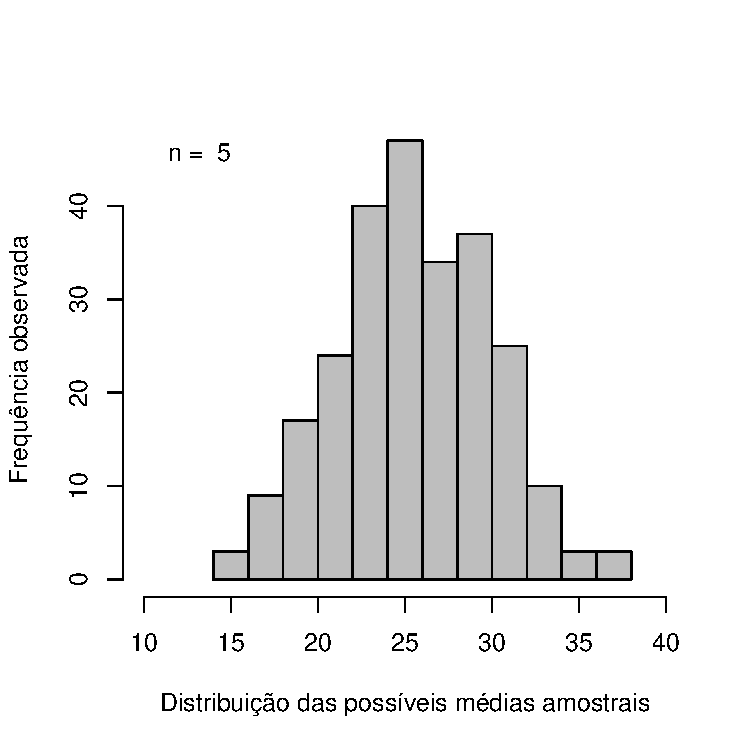
\includegraphics{probest-cambientais_files/figure-latex/unnamed-chunk-58-1} \end{center}

Se calcularmos a \textbf{média das médias} (\(\overline{\overline{X}}\)), ou seja, somarmos todos estes valores e dividirmos por 252, o resultado será 25.6, que é exatamente o valor da média populacional \(\mu\). Isto têm uma implicação central em inferência estatística. Significa que a média amostral \(\overline{X}\) é um estimador \textbf{acurado} (= \textbf{não-viciado}), pois tende a estimar corretamente o valor da média populacional \(\mu\). Ou seja, o histograma acima está centrado ao redor de \(\mu\), o que significa que \textbf{em média} uma amostra particular tem maior probabilidade de expressar um \(\overline{X}\) próxima ao valor populacional.

\hypertarget{precisuxe3o}{%
\subsection{Precisão}\label{precisuxe3o}}

Suponha agora que tomemos ao acaso amostras com \(n = 7\) desta mesma população. Existem ao todo:

\[{{10}\choose{7}} \frac{10!}{(10-7)! \times 7!} = 120\]

amostras diferentes de tamanho \(n = 7\) que podem ser retiradas de uma população de tamanho \(n = 10\). Se tomarmos estas 120 amostras e calcularmos suas respectivas médias amostrais, teremos os resultados abaixo:

\begin{tabular}{r|r|r|r|r|r|r|r|r|r|r|r}
\hline
18.6 & 20.3 & 20.4 & 20.6 & 20.4 & 20.6 & 20.7 & 22.3 & 22.4 & 22.6 & 20.6 & 20.7\\
\hline
20.9 & 22.4 & 22.6 & 22.7 & 22.6 & 22.7 & 22.9 & 24.6 & 21.7 & 21.9 & 22.0 & 23.6\\
\hline
23.7 & 23.9 & 23.7 & 23.9 & 24.0 & 25.7 & 23.9 & 24.0 & 24.1 & 25.9 & 26.0 & 22.4\\
\hline
22.6 & 22.7 & 24.3 & 24.4 & 24.6 & 24.4 & 24.6 & 24.7 & 26.4 & 24.6 & 24.7 & 24.9\\
\hline
26.6 & 26.7 & 25.7 & 25.9 & 26.0 & 27.7 & 27.9 & 28.0 & 23.0 & 23.1 & 23.3 & 24.9\\
\hline
25.0 & 25.1 & 25.0 & 25.1 & 25.3 & 27.0 & 25.1 & 25.3 & 25.4 & 27.1 & 27.3 & 26.3\\
\hline
26.4 & 26.6 & 28.3 & 28.4 & 28.6 & 27.0 & 27.1 & 27.3 & 29.0 & 29.1 & 29.3 & 30.4\\
\hline
24.0 & 24.1 & 24.3 & 25.9 & 26.0 & 26.1 & 26.0 & 26.1 & 26.3 & 28.0 & 26.1 & 26.3\\
\hline
26.4 & 28.1 & 28.3 & 27.3 & 27.4 & 27.6 & 29.3 & 29.4 & 29.6 & 28.0 & 28.1 & 28.3\\
\hline
30.0 & 30.1 & 30.3 & 31.4 & 28.6 & 28.7 & 28.9 & 30.6 & 30.7 & 30.9 & 32.0 & 32.7\\
\hline
\end{tabular}

\begin{center}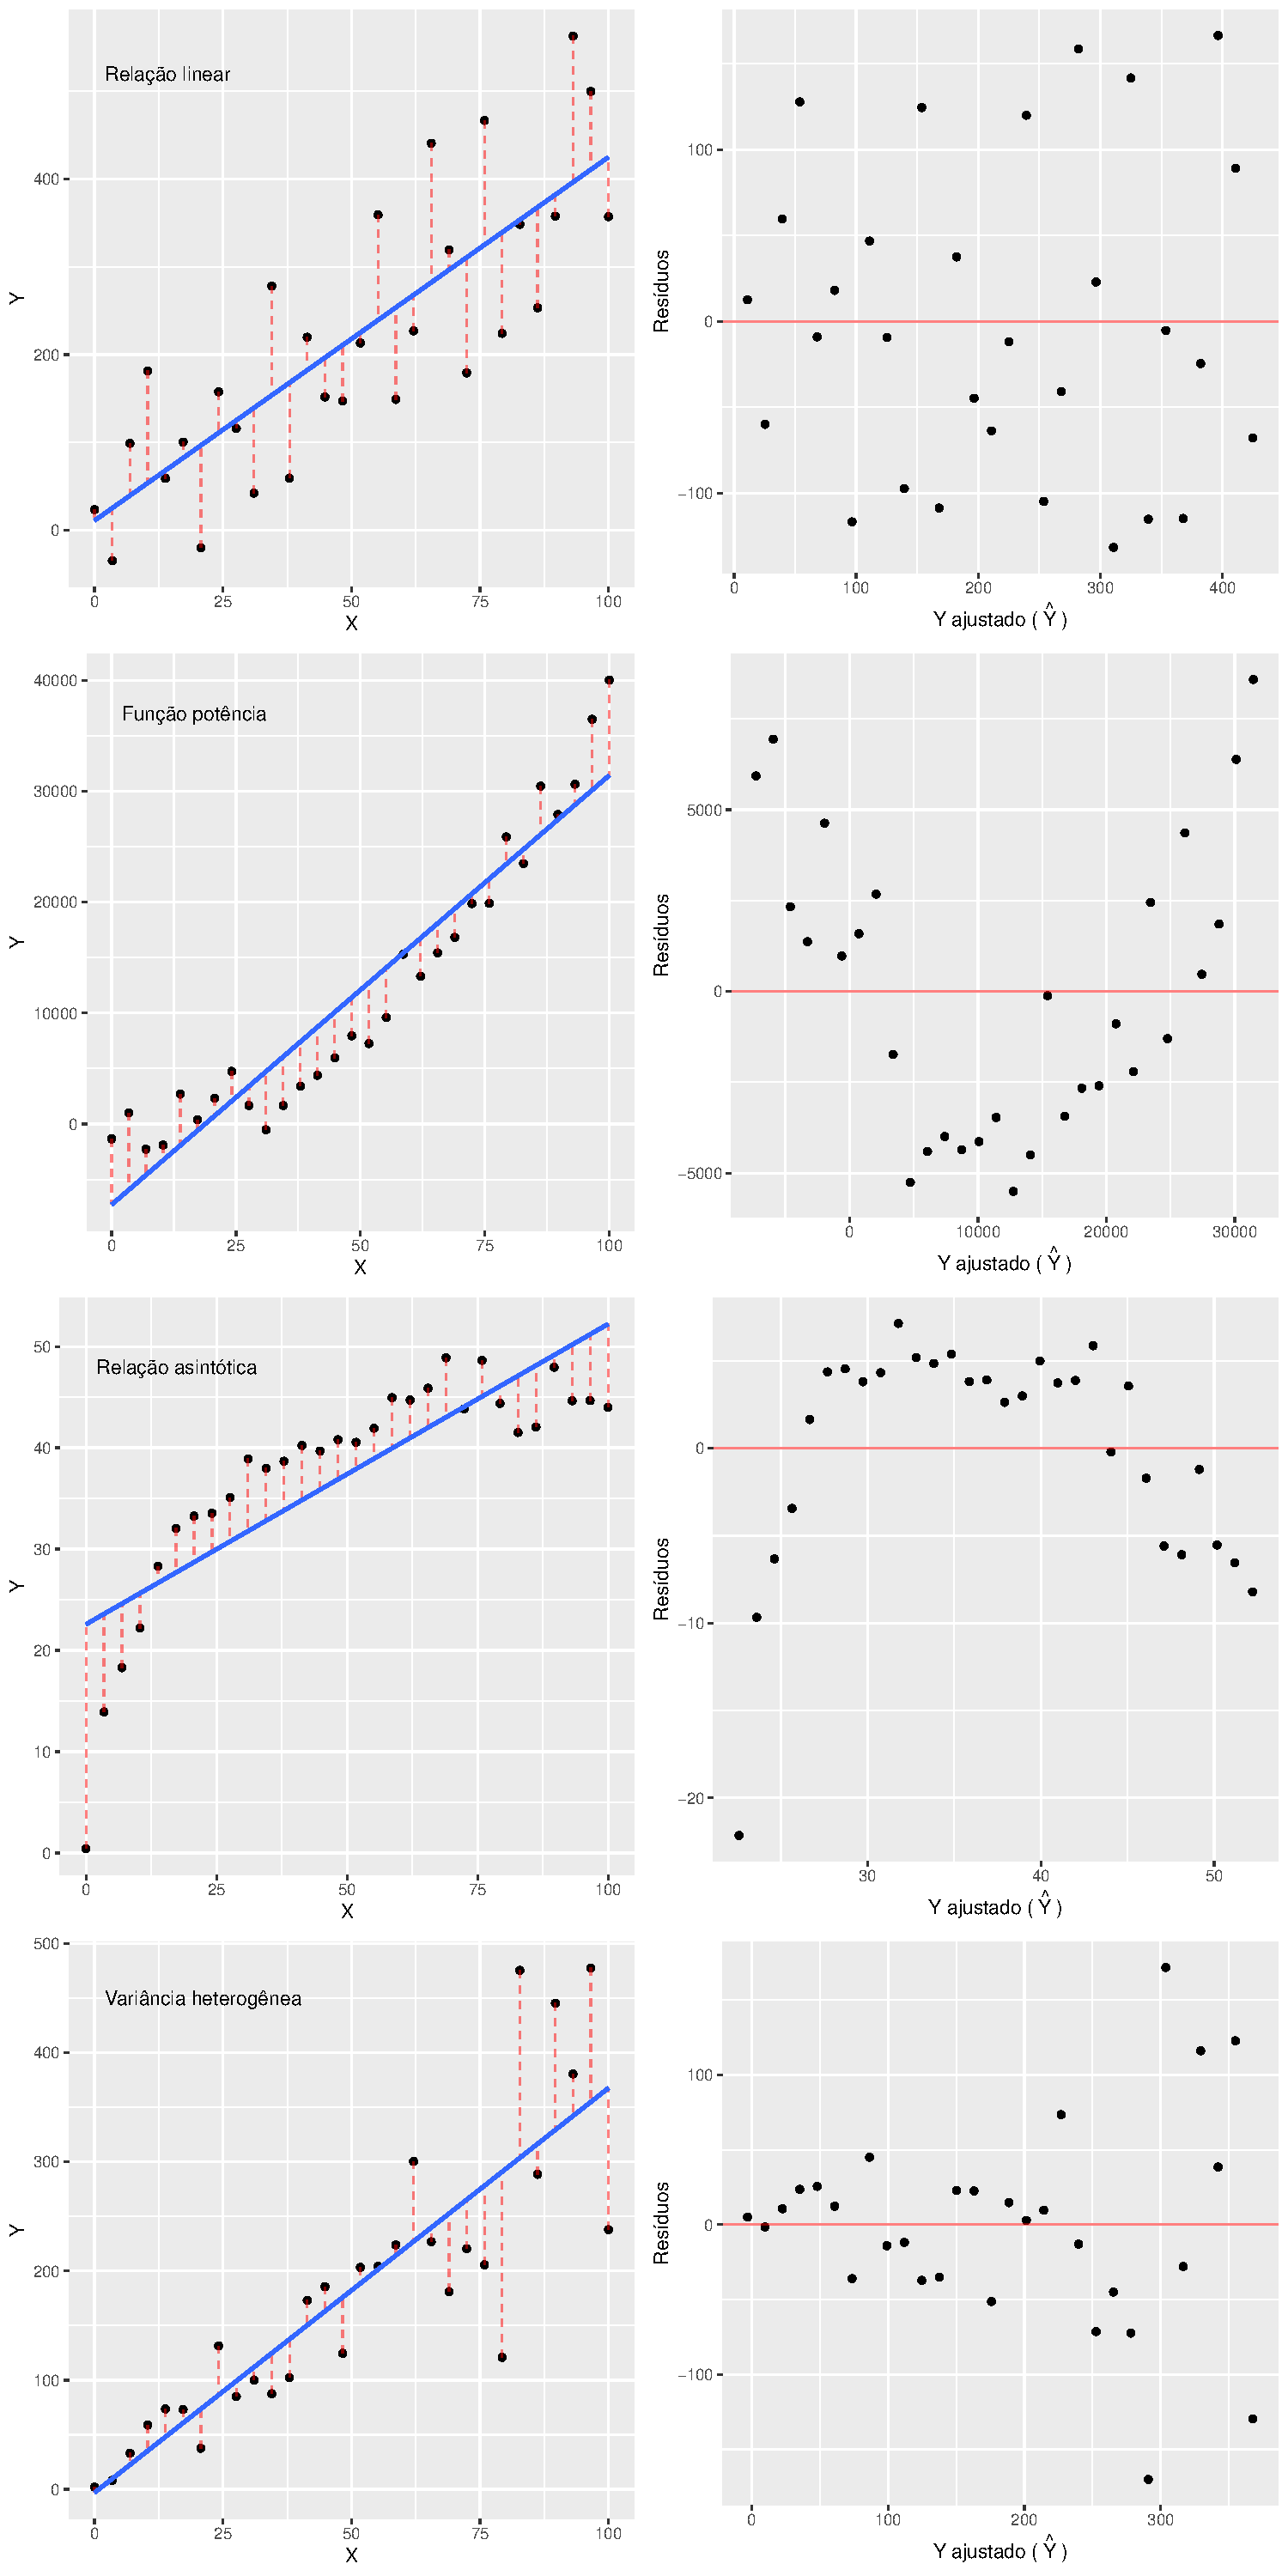
\includegraphics{probest-cambientais_files/figure-latex/unnamed-chunk-61-1} \end{center}

Se compararmos os histogramas com \(n = 5\) e \(n = 7\), veremos que as duas geram estimativas acuradas, pois \(\overline{\overline{X}} = \mu\). No entando, o \textbf{intervalo de variação} é menor para amostras de tamanho \(n = 7\). Para esta figura, os valores estão mais concentrados ao redor da média. Portanto, à medida que aumenta o tamanhol amostral, diminui a disparsão das médias amostrais ao redor de \(\mu\). Assim, para amostras grandes torna-se mais \textbf{improvável} obter uma média amostral distante da média populacional. Disemoz então que Conforme aumenta o tamanho amostral, aumenta a precisão do estimador.

\hypertarget{erro-padruxe3o-da-muxe9dia}{%
\subsection{Erro padrão da média}\label{erro-padruxe3o-da-muxe9dia}}

A precisão de um estimador pode ser medida pelo \textbf{Erro padrão da média} (\(\sigma_{\overline{X}}\)) que pode ser calculado por:

\[\sigma_{\overline{X}} = \frac{\sigma}{\sqrt{n}}\]

O erro padrão da média é o desvio padrão de \textbf{todas} as médias amostrais que poderiam ser obtidas de uma amostra com tamanho \(n\). Para nosso exemplo com \(n = 5\), \(\sigma_{\overline{X}}\) = 0.76, enquanto para \(n = 7\), \(\sigma_{\overline{X}}\) = 0.33. Dizemos que o último exemplo provê um estimador \textbf{mais preciso}.

Como na vida real não temos como o obter \textbf{todas} as médias amostrais da população, não temos como saber com exatidão qual será o valor de \(\sigma_{\overline{X}}\). No entanto, dado que temos uma amostra particular, podemos \textbf{estimá-lo} a partir de \(\sigma_{\overline{X}}\) a partir de:

\[s_{\overline{X}} = \frac{s}{\sqrt{n}}\]

onde \(s\) é o desvio padrão da amostra particular.

Após esta discussão, podemos representar os conceitos de precisão e acurária mostrados utilizando histogramas de distribuição de frequência para as médias amostrais. Vemos portanto que precisão e acurária têm relação respectivamente, com o \textbf{grau de variabilidade} das médias amostrais e com as \textbf{distâncias esperadas} de \(\mu\).

\begin{figure}

{\centering 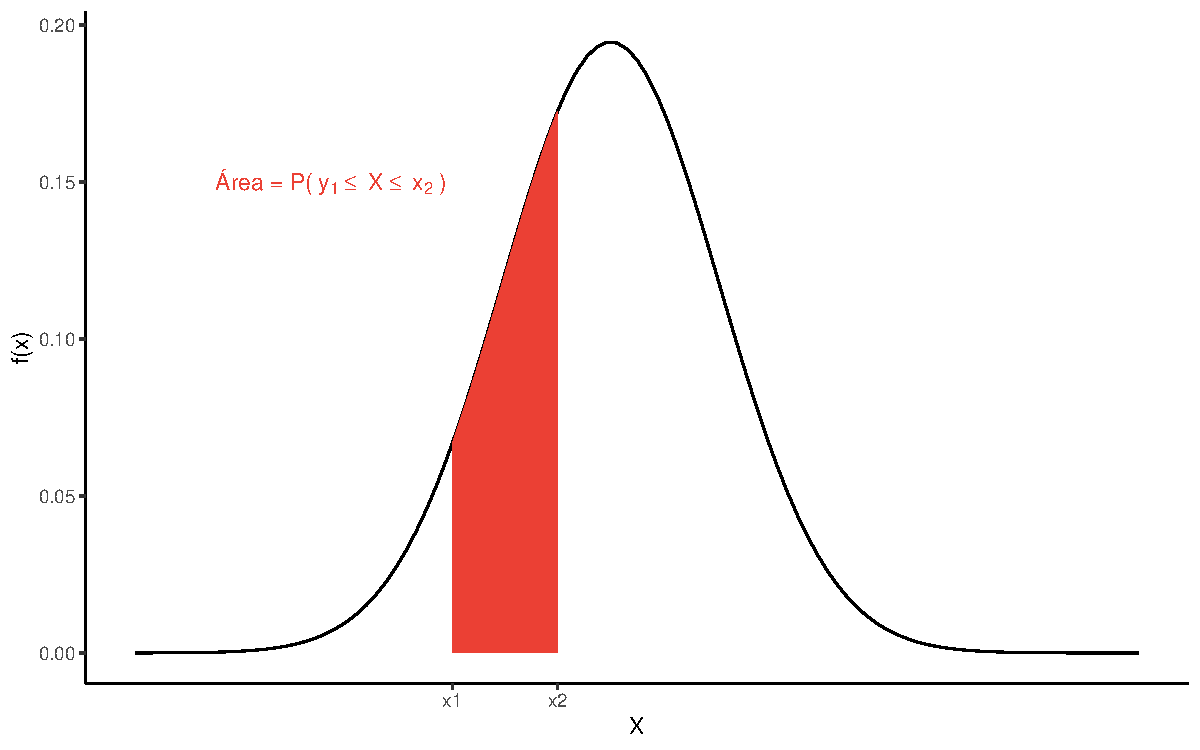
\includegraphics{probest-cambientais_files/figure-latex/unnamed-chunk-62-1} 

}

\caption{Representação dos conceitos de precisão e acurácia. A linha vermelha tracejada representa a média populacional e os histogramas representam a distribuição de todas a médias amostrais com tamanho n desta população. A: estimativas acuradas e não-precisas; B: acuradas e precisas; C: não-acuradas e precisas; D: não-acuradas e não-precisas.}\label{fig:unnamed-chunk-62}
\end{figure}

\hypertarget{normdist}{%
\chapter{Alguns fenômenos têm distribuição normal}\label{normdist}}

No capítulo \ref{amostrmedias}, a distribuição das médias amostrais foi apresentada como um histograma em forma de sino. Este histograma é \textbf{simétrico} ao redor de \(\mu\). A curva teórica que representa esta distribuição é chamada de \textbf{Distribuição Normal} ou \textbf{Distribuição Gaussiana}, ou \textbf{Distribuição Normal de Probabilidades}.

Um dos motivos que tornam a distribuição normal de probabilidades central em estatística é a percepção de que muitos fenômenos naturais podem ser descritos por este padrão. Veja o histograma de alturas de 136 alunos da turma de Introdução a Estatística de 2019 do curso de Bacharelado Interdisciplinar em Ciências do Mar (UNIFESP) (figura à esquerda). A linha sobre este histograma representa a distribuição normal teórica. À direita na mesma figura está um histograma da temperatura média anual em uma cidade americana, onde também foi sobreposta uma curva teórica Gaussiana. Embora estes dados descrevam fenômenos completamente distintos, a distribuição normal se adequa razoavelmente bem aos dois histogramas.

\begin{figure}

{\centering 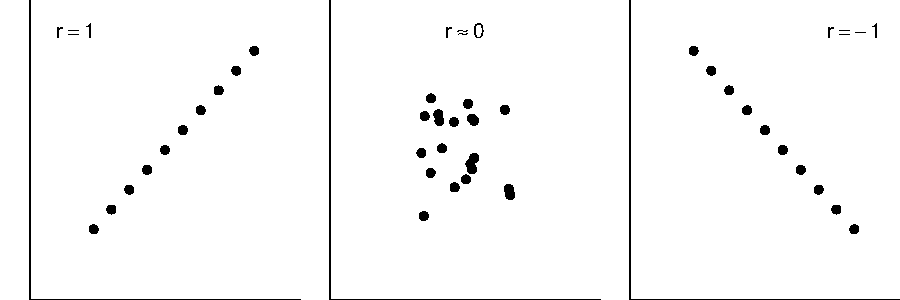
\includegraphics{probest-cambientais_files/figure-latex/unnamed-chunk-65-1} 

}

\caption{Altura (m) de alunos de um curso de estatística e temperatura média anual de uma cidade americana}\label{fig:unnamed-chunk-65}
\end{figure}

As técnicas de estatística descritiva apresentadas anteriormente (capítulos \ref{descrit} e \ref{posicao}) nos permitem entender os padrões resultantes de fenômenos que já aconteceram. Seria interessante no entanto, se pudessemos utilizar estes padrões para realizar predições sobre o que \textbf{poderá acontecer}. Em estatística, a predição se torna possível pelo uso de \textbf{modelos probabilísticos}, dentre os quais a distribuição normal é um dos mais importantes.

Modelos probabilísticos são definidos por \textbf{funções de probabilidade}. A variável envolvida neste modelo é denominada de \textbf{variável aleatória} (capítulos \ref{va} e \ref{vacont}). Uma variável aleatória resulta de um \textbf{experimento aleatório}. Estou utilizando o termo experimento aleatório em como um procedimento científico que nos provê informações sobre algum fenômeno de interesse. Neste sentido, medir a altura de um aluno, tomar a temperatura atual de uma cidade, medir a taxa de crescimento de uma bactéria são todos experimentos aleatórios. A questão relevante nestes experimentos é que \emph{antes} de ser finalizado, não temos certeza sobre qual será seu resultado. Embora não saibamos qual será o resultado exato do experimento, podemos prever nos basear em algum modelo probabilidades para prever a chance deste resultado estar dentro de determinados limites. O papel de um modelo probabilísticos é portanto, delimitar a incerteza ao redor dos resultados possíveis de um experimento aleatório.

Ao medir a altura de um aluno, podemos supor que existe grande probabilidade desta ficar abaixo de \(1,9\) m. Supomos isto pois temos conhecimento de que a altura de maior parte das pessoas está abaixo deste limite. Entretanto, se quisermos atribuir um valor de probabilidade a esta suposição devemos:

\begin{quote}
\begin{enumerate}
\def\labelenumi{\arabic{enumi}.}
\tightlist
\item
  Assumir que a variável altura segue um determinado modelo de probabilidades, e
\item
  Utilizar dados de um experimento para estimar os parâmetros deste modelo a fim de calcularmos a probabilidade \(P(X \le 1,9)\). Discutiremos isto em detalhes a partir do capítulo \ref{va} para diferentes tipos de experimentos e de modelos de probabilidades.
\end{enumerate}
\end{quote}

\hypertarget{o-modelo-normal-de-probabilidades}{%
\section{O modelo normal de probabilidades}\label{o-modelo-normal-de-probabilidades}}

O modelo normal de probabilidades é uma função dada por:

\(f(x) = \frac{1}{\sqrt(2\pi\sigma^2)}e^{-\frac{1}{2}(\frac{y-\mu}{\sigma})^2}\), \(y \in \mathbb{R} | -\infty \le x \le +\infty\)

A expressão envolve as quantias \(\mu\) e \(\sigma\), definidas como os \textbf{parâmetros} da distribuição que representam respectivamente sua média e o desvio padrão. Pdemos apontar que uma variável aleatória \(X\) tem distribuição normal por meio de:

\(X \sim \mathcal{N}(\mu,\,\sigma^2)\)

A média de uma distribuição normal é o ponto central da curva e o desvio padrão mede o grau de espalhamento das observações ao redor de \(\mu\). Para valores baixos de \(\sigma\), a maioria das observações estará próxima a \(\mu\), enquanto para valores altos de \(\sigma\) as observações estarão mais distantes de \(\mu\). Deste modo, ao variar \(\mu\) e \(\sigma\) podemos ter uma infinidade de distribuições normais.

\begin{center}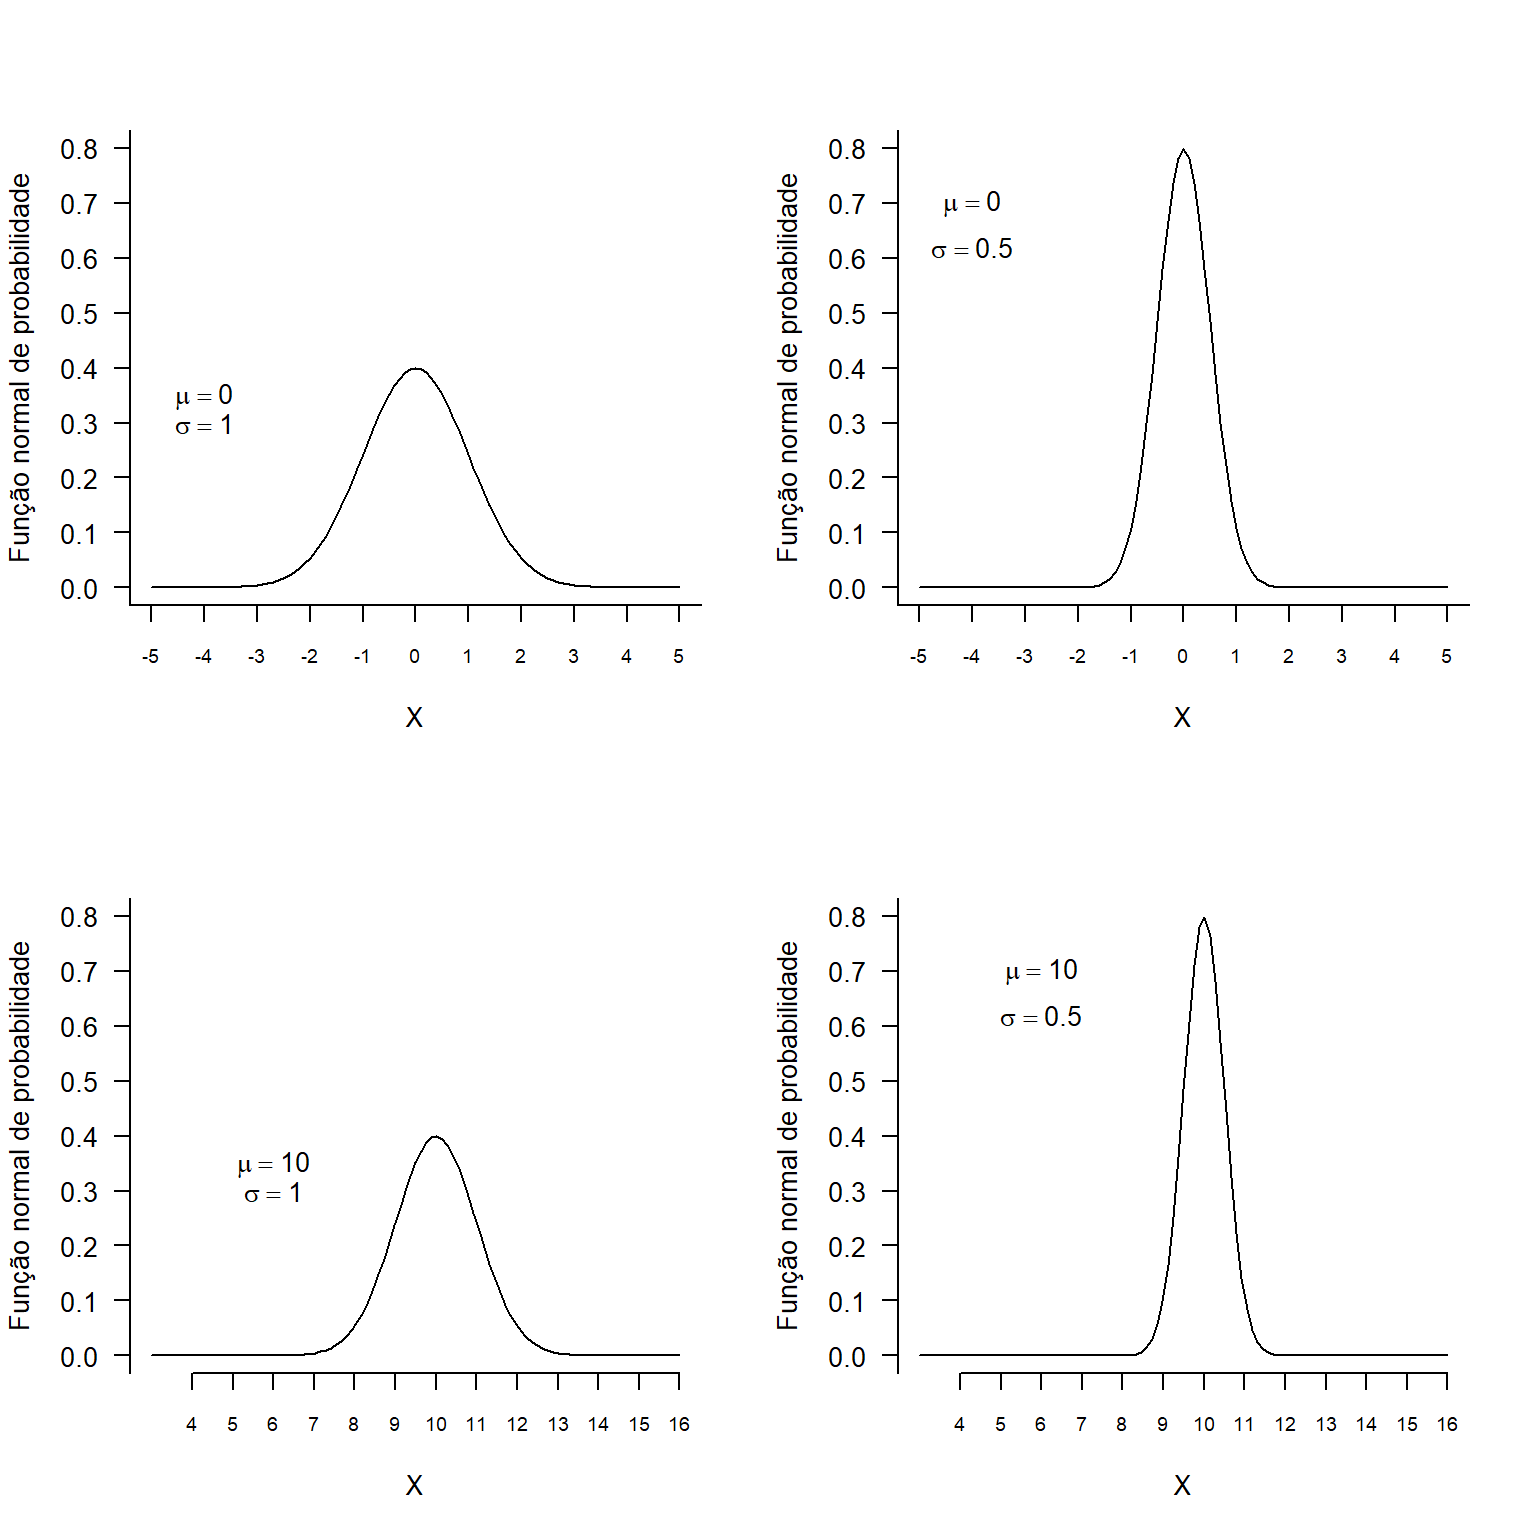
\includegraphics{probest-cambientais_files/figure-latex/unnamed-chunk-66-1} \end{center}

Se as mensurações sobre um determinado fenômeno apresentarem um padrão em forma de sino, podemos buscar a melhor combinação de \(\mu\) e \(\sigma\) e descrever o fenômeno por meio de um modelo normal. Ao fazer isto, poderemos utilizar este modelo para entender quais são as probabilidade de eventos futuros estarem em diferentes faixas de valores. No caso das alturas dos alunos por exemplo, vemos que a probabilidade de um aluno ter mais de 2 metros ou menos de 1,5m é extremamente baixa.

\hypertarget{entendendo-a-funuxe7uxe3o-normal-de-densidade-de-probabilidade}{%
\section{Entendendo a função normal de densidade de probabilidade}\label{entendendo-a-funuxe7uxe3o-normal-de-densidade-de-probabilidade}}

A função \(f(x) = \frac{1}{\sqrt(2\pi\sigma^2)}e^{-\frac{1}{2}(\frac{y-\mu}{\sigma})^2}\) não oferece diretamente a probabilidade de \(x\) assumir determinado intervalo. \(f(x)\) é uma \textbf{função de densidade de probabilidade}. Vamos utilizá-la para encontrar \(f(x)\) utilizando os dados de altura dos alunos do BICT Mar.~Vamos assumir que os parâmetros do modelo normal são:

\(\mu = 1.7\)

\(\sigma = 0.11\)

Para um \(x = 1.6\):

\(f(1.6) = \frac{1}{\sqrt(2\pi \times0.11^2)}e^{-\frac{1}{2}(\frac{1.6 - 1.7}{0.11})^2} = 2.399\)

Este resultado corresponde ao ponto em \(x\) no gráfico da distribuição normal. Assim, se calcularmos \(f(x)\) para diferentes pontos em \(x\) teremos um esboço da função de densidade normal.

\begin{center}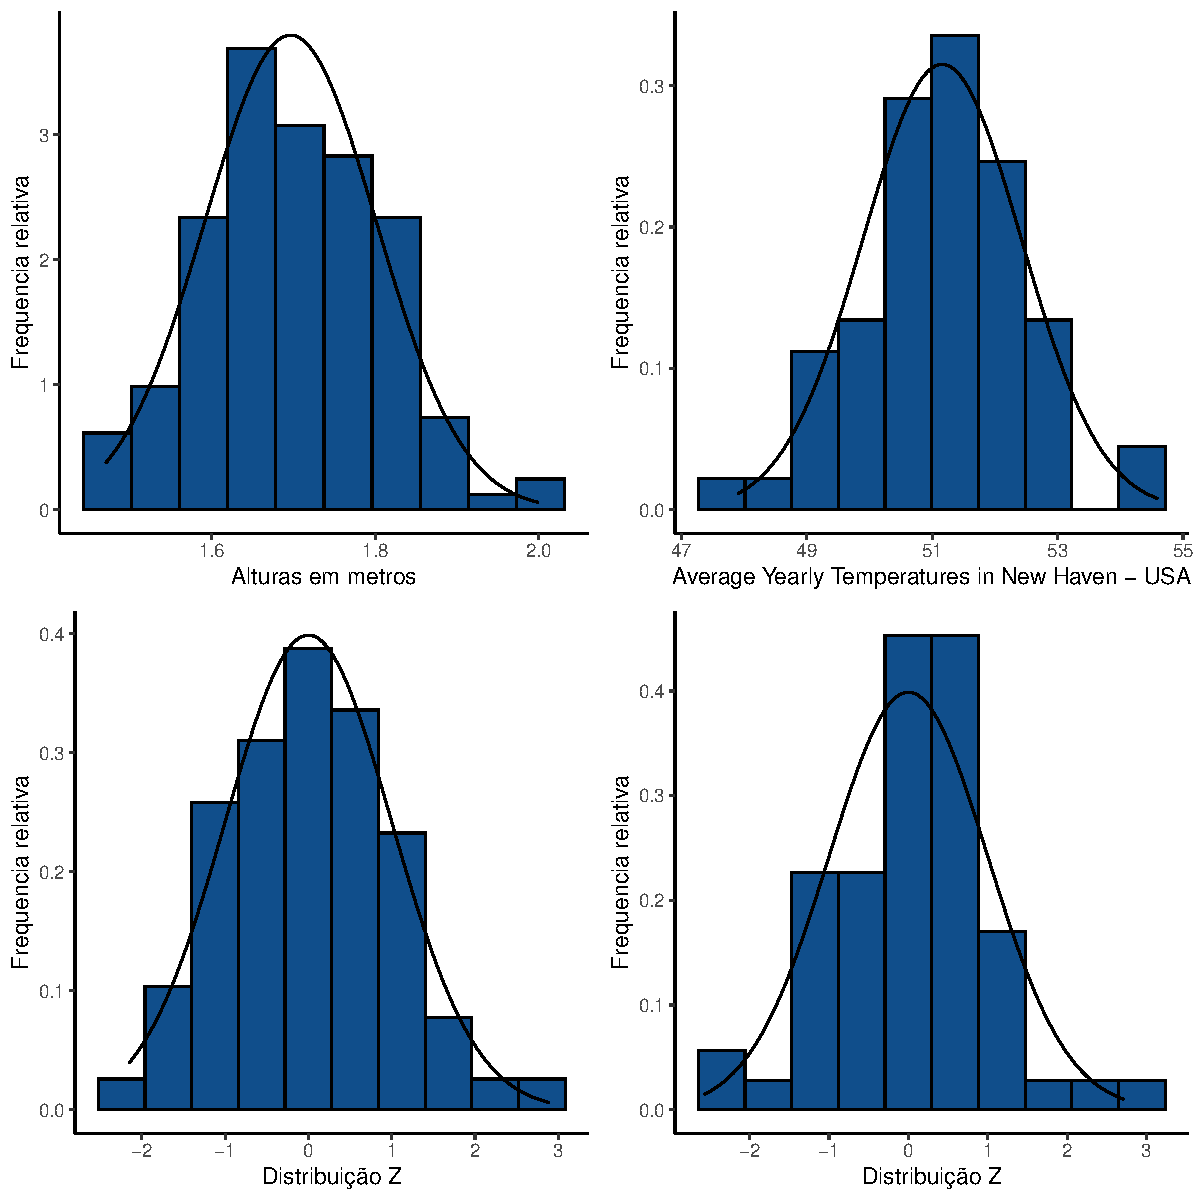
\includegraphics{probest-cambientais_files/figure-latex/unnamed-chunk-68-1} \end{center}

No R, os resultados acima podem ser obtidos com a função \texttt{dnorm}, que fornece um modo simples para calcularmos \(f(x)\) para a distribuição normal. Nesta função `d' vem de \emph{densidade} da distribuição normal.

\begin{Shaded}
\begin{Highlighting}[]
\NormalTok{mu }\OtherTok{\textless{}{-}} \FloatTok{1.7}
\NormalTok{dp }\OtherTok{\textless{}{-}} \FloatTok{0.11}
\FunctionTok{dnorm}\NormalTok{(}\FloatTok{1.5}\NormalTok{, }\AttributeTok{mean =}\NormalTok{ mu, }\AttributeTok{sd =}\NormalTok{ dp)}
\end{Highlighting}
\end{Shaded}

\begin{verbatim}
## [1] 0.6945048
\end{verbatim}

Se quisermos obter \(f(x)\) para múltiplos valores de \(x\) podemos fazer:

\begin{Shaded}
\begin{Highlighting}[]
\NormalTok{x }\OtherTok{\textless{}{-}} \FunctionTok{c}\NormalTok{(}\FloatTok{1.4}\NormalTok{, }\FloatTok{1.5}\NormalTok{, }\FloatTok{1.6}\NormalTok{, }\FloatTok{1.7}\NormalTok{)}
\FunctionTok{dnorm}\NormalTok{(x, }\AttributeTok{mean =}\NormalTok{ mu, }\AttributeTok{sd =}\NormalTok{ dp)}
\end{Highlighting}
\end{Shaded}

\begin{verbatim}
## [1] 0.0879777 0.6945048 2.3991470 3.6267480
\end{verbatim}

\hypertarget{fazendo-prediuxe7uxf5es-com-a-funuxe7uxe3o-normal-de-densidade}{%
\section{Fazendo predições com a função normal de densidade}\label{fazendo-prediuxe7uxf5es-com-a-funuxe7uxe3o-normal-de-densidade}}

Por ser uma função de probabilidade, a área abaixo de \(f(x)\) soma 1. Assim, se desejamos obter probabilidade de uma variável estar dentro de um determinado limite, devemos calcular a \textbf{área abaixo da curva} para este limite. Por exemplo, a probabilidade de uma observação em \(X\) estar entre \(x_1\) e \(x_2\) será:

\begin{center}
\includegraphics{probest-cambientais_files/figure-latex/unnamed-chunk-71-1} \end{center}

Você lembra-se que a área abaixo de uma função matemática é dada pela integral definida desta função.

\[P(x_1 \le X \le x_2) = \int_{x_1}^{x_2}f(x) dx\]

Usando o R, a probabilidade de amostrarmos um aluno que tenha entre menos de 1.5 metros pode ser obtida por meio da função \texttt{pnorm}:

\begin{Shaded}
\begin{Highlighting}[]
\NormalTok{mu }\OtherTok{\textless{}{-}} \FloatTok{1.7}
\NormalTok{dp }\OtherTok{\textless{}{-}} \FloatTok{0.11}
\FunctionTok{pnorm}\NormalTok{(}\AttributeTok{q =} \FloatTok{1.5}\NormalTok{, }\AttributeTok{mean =}\NormalTok{ mu, }\AttributeTok{sd =}\NormalTok{ dp, }\AttributeTok{lower.tail =} \ConstantTok{TRUE}\NormalTok{)}
\end{Highlighting}
\end{Shaded}

\begin{verbatim}
## [1] 0.03451817
\end{verbatim}

Os argumentos desta função são (veja o menu de ajuda digitando \texttt{?pnorm} no Console do R):

\begin{quote}
q: o valor de \(x\)
\end{quote}

\begin{quote}
mean: média \(\mu\) da função normal
\end{quote}

\begin{quote}
sd: desvio padrão \(\sigma\) da função normal
\end{quote}

\begin{quote}
lower.tail: se a função irá retornar a probabilidade abaixo (TRUE) ou acima (FALSE) de q
\end{quote}

Se quisermos a probabilidade \(P(X \ge 1.5)\) alteramos o parâmetro \texttt{lower.tail}

\begin{Shaded}
\begin{Highlighting}[]
\FunctionTok{pnorm}\NormalTok{(}\AttributeTok{q =} \FloatTok{1.5}\NormalTok{, }\AttributeTok{mean =}\NormalTok{ mu, }\AttributeTok{sd =}\NormalTok{ dp, }\AttributeTok{lower.tail =} \ConstantTok{FALSE}\NormalTok{)}
\end{Highlighting}
\end{Shaded}

\begin{verbatim}
## [1] 0.9654818
\end{verbatim}

Se desejamos obter a probabilidade de \(x\) estar \textbf{entre} 1.5m e 1.7m podemos fazer: \[P(1.5 \le X \le 1.7) = P(X \le 1.7) - P(X \le 1.5)\]

No R temos:

\begin{Shaded}
\begin{Highlighting}[]
\NormalTok{p1 }\OtherTok{\textless{}{-}} \FunctionTok{pnorm}\NormalTok{(}\AttributeTok{q =} \FloatTok{1.7}\NormalTok{, }\AttributeTok{mean =}\NormalTok{ mu, }\AttributeTok{sd =}\NormalTok{ dp, }\AttributeTok{lower.tail =} \ConstantTok{TRUE}\NormalTok{)}
\NormalTok{p2 }\OtherTok{\textless{}{-}} \FunctionTok{pnorm}\NormalTok{(}\AttributeTok{q =} \FloatTok{1.5}\NormalTok{, }\AttributeTok{mean =}\NormalTok{ mu, }\AttributeTok{sd =}\NormalTok{ dp, }\AttributeTok{lower.tail =} \ConstantTok{TRUE}\NormalTok{)}
\NormalTok{pfinal }\OtherTok{\textless{}{-}}\NormalTok{ p1 }\SpecialCharTok{{-}}\NormalTok{ p2}

\NormalTok{pfinal}
\end{Highlighting}
\end{Shaded}

\begin{verbatim}
## [1] 0.4654818
\end{verbatim}

ou simplesmente

\begin{Shaded}
\begin{Highlighting}[]
\FunctionTok{diff}\NormalTok{(}\FunctionTok{pnorm}\NormalTok{(}\AttributeTok{q =} \FunctionTok{c}\NormalTok{(}\FloatTok{1.7}\NormalTok{, }\FloatTok{1.5}\NormalTok{),}
           \AttributeTok{mean =}\NormalTok{ mu,}
           \AttributeTok{sd =}\NormalTok{ dp,}
           \AttributeTok{lower.tail =} \ConstantTok{TRUE}\NormalTok{)}
\NormalTok{     )}
\end{Highlighting}
\end{Shaded}

\begin{verbatim}
## [1] -0.4654818
\end{verbatim}

Aqui estão representados cada um dos intervalos calculados.

\begin{center}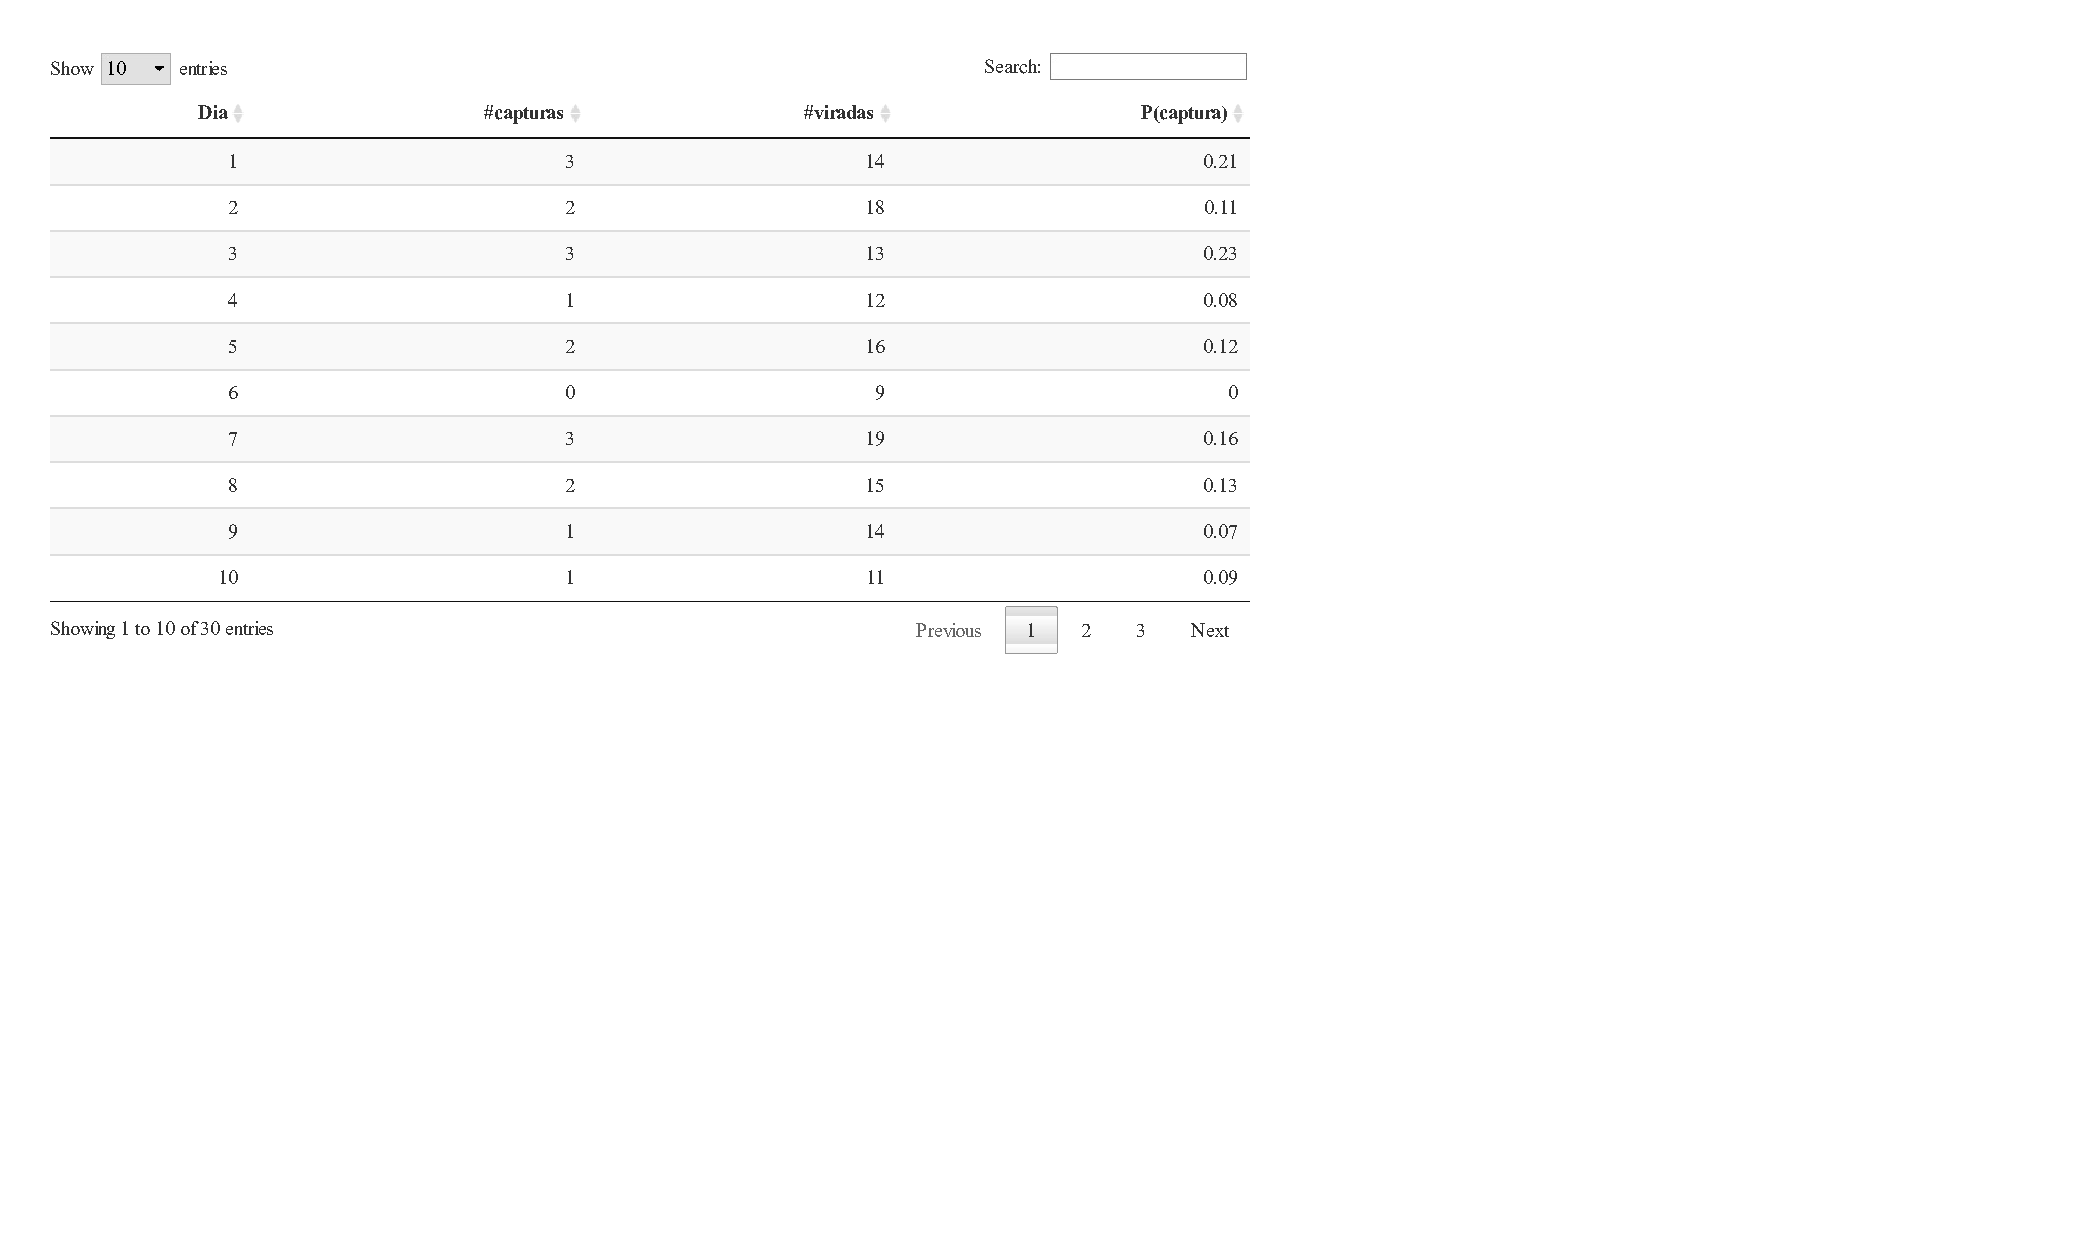
\includegraphics{probest-cambientais_files/figure-latex/unnamed-chunk-76-1} \end{center}

\hypertarget{a-distribuiuxe7uxe3o-normal-padronizada}{%
\section{A distribuição normal padronizada}\label{a-distribuiuxe7uxe3o-normal-padronizada}}

A integral para a função normal é difícil de ser calculada pois não tem solução analítica. Isto era um problema para os cientistas até meados do século XX de precisariam calcular valores de probabilidade para diferentes combinações de \(\mu\) e \(\sigma\). Naquele momento, a solução para facilitar a vida dos pesquisadores foi criar uma tabela descrevendo estas probabilidades em uma distribuição normal \textbf{padronizada}, ou seja para valores particulares de \(\mu\) e \(\sigma\). Padronizar aqui, significa transfomar cada valor \(x_i\) de modo que as observações resultantes tenham média igual a 0 e desvio padrão igual a 1.

Esta transformação é realizada transformando cada observação \(x_i\) em um valor de \(z_i\) por meio da expressão.

\[z_i = \frac{x_i - \bar{x}}{s}\]
Lembre-se que no capítulo \ref{posicao} apresentamos \(z_i\) como uma \textbf{medida de posição}, uma vez que representa uma medida \textbf{relativa} à média e ao desvio padrão de um conjunto de dados particular. Por exemplo, um valor de \(z_i = 2\) significa que a observação original \(x_i\) está 2 desvios padrões \textbf{acima} da média \(\overline{x}\).

\begin{quote}
\emph{Releita o tópico ``Interpretando o valor de Z''} (Capítulo \ref{posicao}).
\end{quote}

Esta transformação é útil, pois ainda que seja difícil calcular as probabilidades para uma variável aleatória \(X\), após a transformação teremos uma variável \(Z\) para a qual os valores de probabilidade estão \textbf{tabelados}. Deste modo, \(Z\) é uma variável aleatória com \(\overline{z} = 0\) e \(s = 1\) tal que:

\[Z \sim \mathcal{N}(0,\,1)\]

Para o exemplos sobre altura dos alunos e chuva mensal temos:

\begin{center}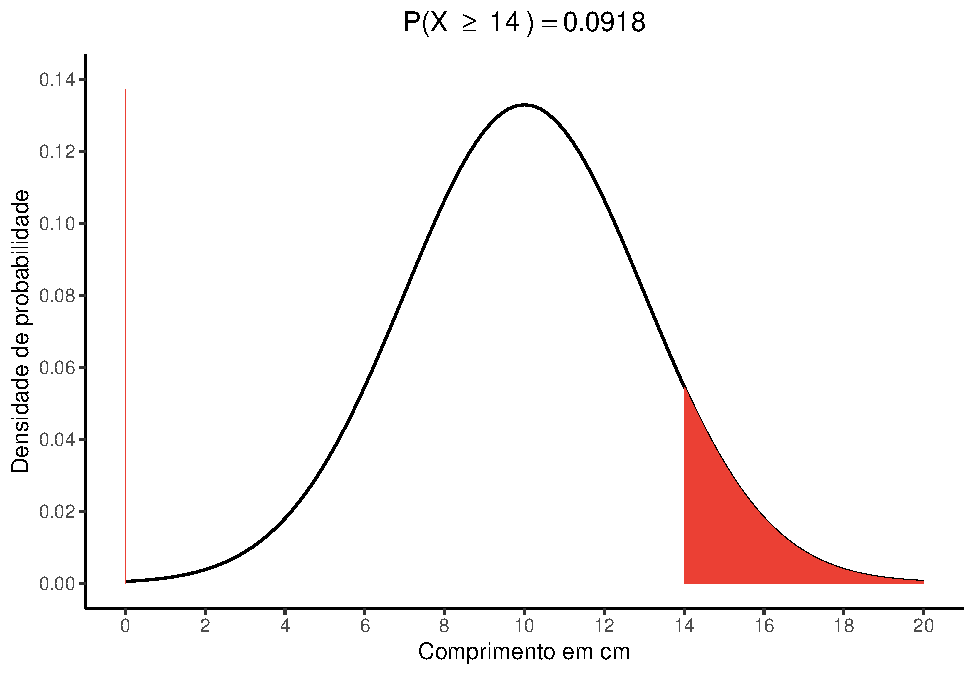
\includegraphics{probest-cambientais_files/figure-latex/unnamed-chunk-77-1} \end{center}

\hypertarget{probabilidades-em-uma-distribuiuxe7uxe3o-normal-padronizada}{%
\subsection{Probabilidades em uma distribuição normal padronizada}\label{probabilidades-em-uma-distribuiuxe7uxe3o-normal-padronizada}}

Nos dois exemplos anteriores, verifica-se que todas as observações estão situadas, aproximadamente, entre \(z = -3\) e \(z = +3\). De fato, a distribuição normal padronizada ou \textbf{distribuição Z} tem propriedades bem conhecidas. Sua média é \(\mu = 0\) e seu desvio padrão é \(\sigma = 1\), fazendo com que a maior parte das observações fique limitada entre \(z = -3\) e \(z = +3\). Para ser exato, podemos descrever as probabilidades de uma observação estar dentro de alguns limites. Por exemplo, \(95\%\) das observações estará entre \(z = -1.96\) e \(z = +1.96\), isto é, \(P(-1.96 \le Z \le +1.96) = 0.95\). De forma similar, \(90\%\) da área central da curva se encontra entre \(z = -1.64\) e \(z = +1.64\). Estes e outros limites na distribuição normal padronizada podem ser verificados na figura abaixo.

\begin{center}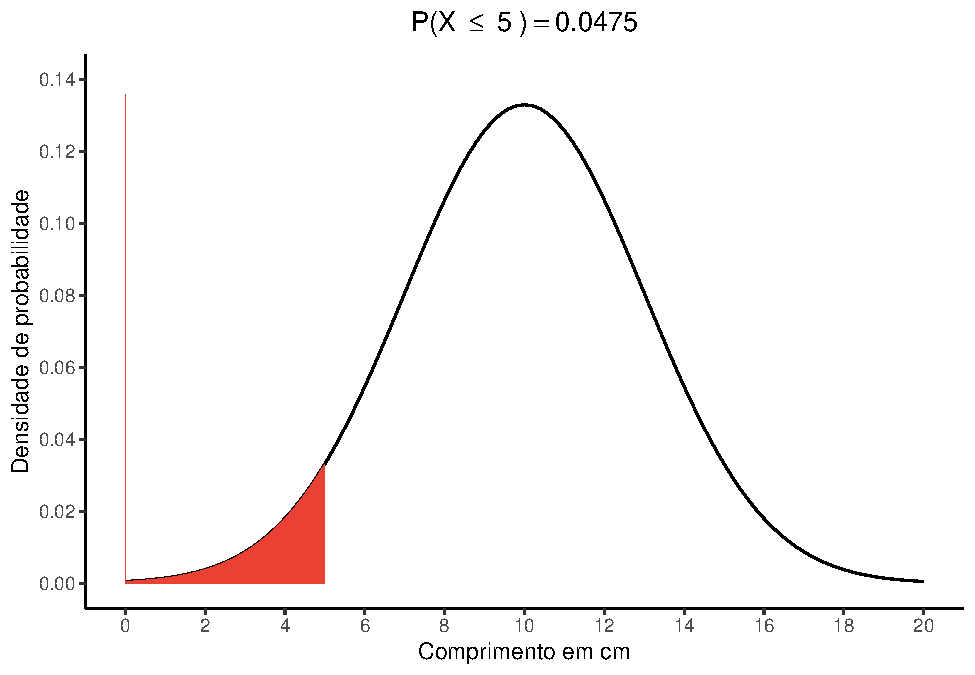
\includegraphics{probest-cambientais_files/figure-latex/unnamed-chunk-78-1} \end{center}

Vamos exemplificar o uso da distribuição Z no cálculo de probabilidades utilizando os dados de altura dos alunos. Para estes dados, iremos encontrar \(P(X \le 1.5)\). Este procedimento consiste de:

\begin{enumerate}
\def\labelenumi{\arabic{enumi}.}
\tightlist
\item
  Transformar \(x = 1.5\) em \(z_{1.5}\) por meio de \(z_{1.5} = \frac{1.5 - 1.7}{0.11} = -1.818\);
\end{enumerate}

\begin{Shaded}
\begin{Highlighting}[]
\NormalTok{mu }\OtherTok{\textless{}{-}} \FloatTok{1.7}
\NormalTok{dp }\OtherTok{\textless{}{-}} \FloatTok{0.11}
\NormalTok{x }\OtherTok{\textless{}{-}} \FloatTok{1.5}
\NormalTok{z\_1}\FloatTok{.5} \OtherTok{\textless{}{-}}\NormalTok{ (x }\SpecialCharTok{{-}}\NormalTok{ mu)}\SpecialCharTok{/}\NormalTok{dp}

\NormalTok{z\_1}\FloatTok{.5}
\end{Highlighting}
\end{Shaded}

\begin{verbatim}
## [1] -1.818182
\end{verbatim}

\begin{enumerate}
\def\labelenumi{\arabic{enumi}.}
\setcounter{enumi}{1}
\tightlist
\item
  Encontrar encontrar \(P(Z \le z_{1.5}) = P(Z \le -1.818)\).
\end{enumerate}

\begin{Shaded}
\begin{Highlighting}[]
\FunctionTok{pnorm}\NormalTok{(}\AttributeTok{q =}\NormalTok{ z\_1}\FloatTok{.5}\NormalTok{, }\AttributeTok{mean =} \DecValTok{0}\NormalTok{, }\AttributeTok{sd =} \DecValTok{1}\NormalTok{, }\AttributeTok{lower.tail =} \ConstantTok{TRUE}\NormalTok{)}
\end{Highlighting}
\end{Shaded}

\begin{verbatim}
## [1] 0.03451817
\end{verbatim}

Compare este resultado com o obtido anteriormente para verificar que é equivalente a \(P(X \le 1.5)\).

\hypertarget{a-transformauxe7uxe3o-z}{%
\subsubsection{\texorpdfstring{A transformação \(Z\)}{A transformação Z}}\label{a-transformauxe7uxe3o-z}}

Do mesmo modo, suponha uma variável aleatória \(X\) nomalmente distribuída conforme \(X \sim \mathcal{N}(\mu,\,\sigma^2)\). Desejamos encontrar \(m\) tal que:

\(P(X \le m) = \alpha\)

\begin{quote}
\(\alpha\) aqui reprsenta um valor de probabilidade qualquer determinada pela área na distribuição normal \textbf{abaixo} de \(m\).
\end{quote}

Ao aplicar a transformação \(Z\) teremos:

\(P(\frac{X - \mu}{\sigma} \le \frac{m - \mu}{\sigma}) = \alpha\)

como \(\frac{X - \mu}{\sigma} = Z\) temos que:

\(P(Z \le \frac{m - \mu}{\sigma}) = \alpha\)

Por meio desta expressão, você pode encontar \(m\) uma vez fornecido \(\alpha\) ou encontrar \(\alpha\), desde que seja fornecido \(m\).

O mesmo vale se quisermos encontrar a probabilidade determinada por um intervalo definido de \(m\) até \(n\) (\(m < n\)). Para isto fazemos:

\(P(m \le X \le n) = \alpha\)

\(P(\frac{m - \mu}{\sigma} \le \frac{X - \mu}{\sigma} \le \frac{n - \mu}{\sigma}) = \alpha\)

\(P(\frac{m - \mu}{\sigma} \le Z \le \frac{n - \mu}{\sigma}) = \alpha\)

\hypertarget{tabela-z}{%
\subsection{\texorpdfstring{Tabela \(Z\)}{Tabela Z}}\label{tabela-z}}

Ao utilizarmos um software estatístico não é necessário fazer esta transformação. A transformação \(Z\) era necessária na ausência de ferramentas computacionais, ou seja, quando a única opção viável era utilizarmos a Tabela Z para evitar cálculos tediosos para cada combinação de \(\mu\) e \(\sigma\).

A tabela disponibiliza os valores de probabilidade para um grande número de valores de \(Z\) e é apresentada na grande maioria dos livros de estatística.

Você pode utilizar a Tabela \(Z\) para encontrar \(P(X \le 1.5)\). Note que o valor transformado é \(z_{1.5} = -1.818\). Este será o valor que iremos buscar na tabela. Para isto:

\begin{enumerate}
\def\labelenumi{\arabic{enumi}.}
\item
  Encontre a página que oferece valores \textbf{negativos}, uma vez que \(z_{1.5} < 0\);
\item
  Na coluna 1 desta página (coluna \textbf{z}) encontre a linha \textbf{-1.8} que refere-se à unidade, e à primeira casa decimal de \(z_{1.5}\);
\item
  Encontre a coluna \textbf{0.02} (quarta coluna da tabela \(Z\)) que apresenta a segunda casa decimal de \(z_{1.5}\). Isto nos leva ao valor mais próximo do calculado (\(z_{1.5} = -1.818\)).
\item
  Cruze a \textbf{linha} escolhida no item 3 com a \textbf{coluna} escolhida no item 4. Você irá encontrar o valor \(0,0344\). Este valor e a probabilidade de obtermos um valor de \(z \le 1.5\) na distribuição normal padronizada, ou seja, \(P(Z \le z_{1.5})\). A diferença entre este valor e o encontrado com o R se deve unicamente à limitação da precisão utilizando a Tabela \(Z\).
\end{enumerate}

\hypertarget{exercuxedcios-resolvidos}{%
\section{Exercícios resolvidos}\label{exercuxedcios-resolvidos}}

\hypertarget{distribuiuxe7uxe3o-de-comprimento}{%
\subsection{Distribuição de comprimento}\label{distribuiuxe7uxe3o-de-comprimento}}

As comunidades de peixes em riachos de cabeceira são compostas por espécies de pequeno porte. \emph{Rhamdioglanis transfasciatus} é uma destas espécies, desconhecida do público em geral, porém muito abundante em pequenos riachos bem preservados. Dados de captura sugerem que o tamanho dos indivíduos pode ser razoavelmente bem descrito por um modelo de distribuição normal.

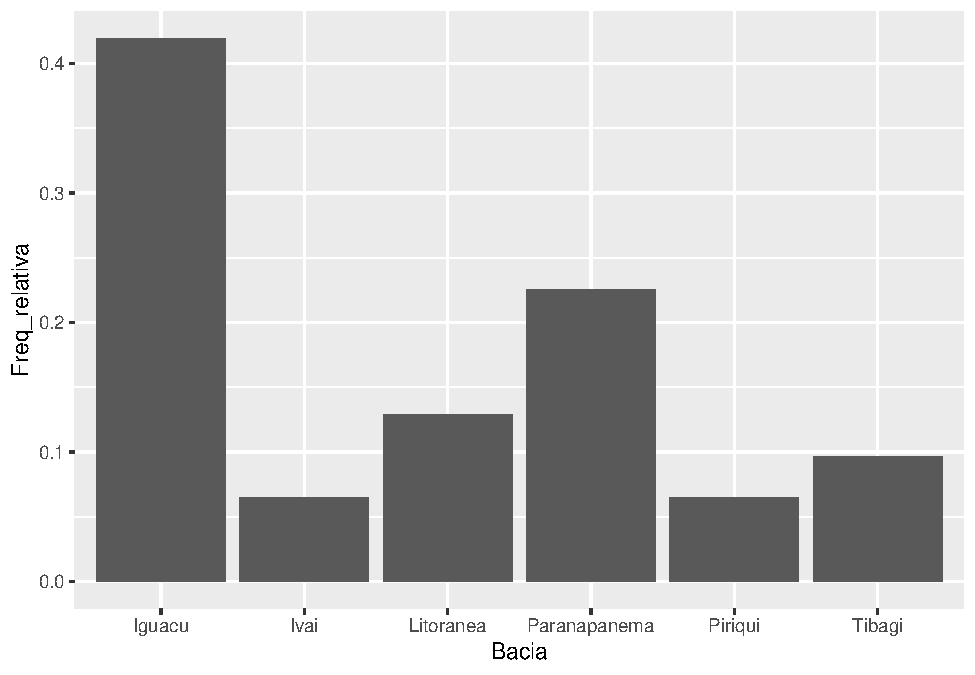
\includegraphics{probest-cambientais_files/figure-latex/unnamed-chunk-83-1.pdf}

Suponha o comprimento desta espécie tenha uma distribuição normal com \(\mu = 10\) cm e \(\sigma = 3\) cm. Encontre:

\begin{enumerate}
\def\labelenumi{\roman{enumi}.}
\tightlist
\item
  A probabilidade de capturar um indivíduo maior de 14 cm de comprimento, \(P(X \ge 14)\).
\item
  A probabilidade de capturar um indivíduo menor de 5 cm de comprimento, \(P(X \le 5)\).
\item
  A probabilidade de encontrar um indivíduo \textbf{entre} 5 e 14 cm, \(P(5 \le X \le 14)\).
\item
  Se um trecho de riacho contém 800 indivíduos, quantos são maiores que 14 cm de comprimento.
\end{enumerate}

\textbf{RESOLUÇÃO}

Para resolver estas questões iremos utilizar a transformação \(Z\).

\textbf{i. Para encontrar \(P(X \ge 14)\):}

Vamos encontrar o respectivo valor de \(Z\) pela transformação

\(z_{14} = \frac{14 - 10}{3} = 1.33\)

Na tabela \(Z\) procuramos a linha que mostra a unidade e \(1^a\) casa decimal de \(1.33\) e em seguida encontramos a coluna que representa a \(2^a\) casa decimal de \(1.33\). Cruzando linha e coluna encontramos o valor \(0,9082\). Note que este valor representa a área \textbf{abaixo} de 1.33, isto é, \(P(Z \le z_{14})\). No entanto, queremos \(P(Z \ge z_{14})\) que representa a área daa curva \textbf{acima} de \(1.33\). Para isto basta fazermos \(1 - 0,9082\).

Deste modo, \(P(Z \ge z_{14}) = 1 - P(Z \le z_{14}) = 1 - 0,9082 = 0.0918\)

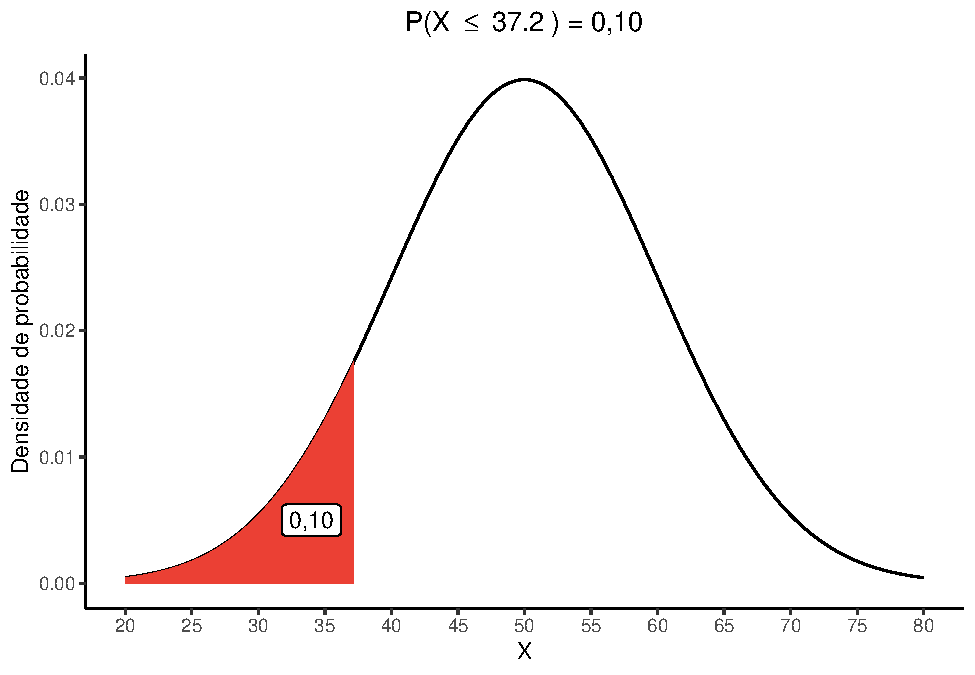
\includegraphics{probest-cambientais_files/figure-latex/unnamed-chunk-86-1.pdf}

\textbf{ii. Para encontrar \(P(X \le 5)\):}

\(z_{5} = \frac{5 - 10}{3} = -1.67\)

Na tabela \(Z\) procuramos a linha que mostra a unidade e \(1^a\) casa decimal de \(-1.67\) e em seguida encontramos a coluna que representa a \(2^a\) casa decimal de \(-1.67\). Cruzando linha e coluna encontramos o valor \(0,0475\) que representa a área desejada.

Deste modo, \(P(X \le 5) = P(Z \le z_{5}) = 0,0475\)

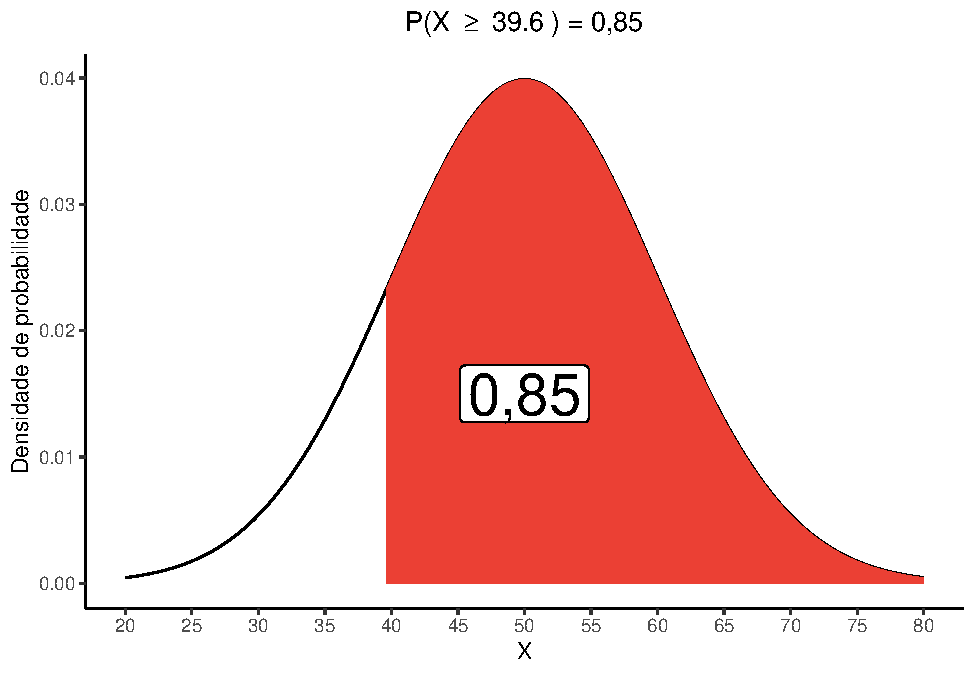
\includegraphics{probest-cambientais_files/figure-latex/unnamed-chunk-87-1.pdf}

\textbf{iii. Para encontrar a área central da curva \(P(5 \le X \le 14)\):}

Vamos subtrair as quantias \(P(Z \le 14) - P(Z \le 5)\)

Estes valores já foram encontrados nos itens anteriores, de modo que basta fazermos:

\(P(5 \le X \le 14) = 0,9082 - 0,0475 = 0.8607\)

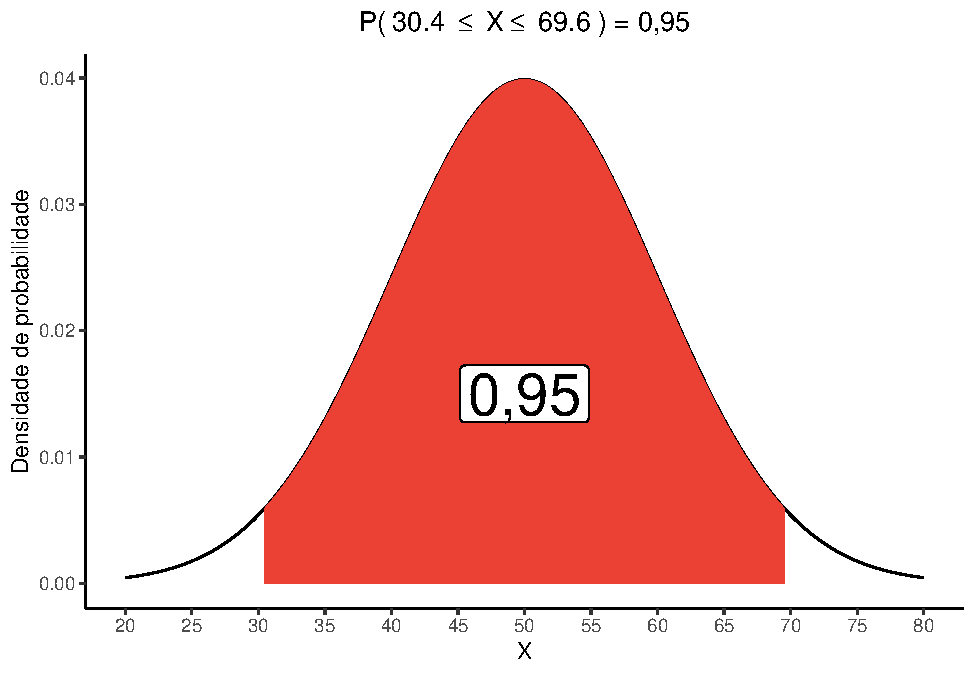
\includegraphics{probest-cambientais_files/figure-latex/unnamed-chunk-88-1.pdf}

\textbf{iv. Indivíduos maiores que 14 cm de comprimento}

Se a proporção de indivíduos acima de 14 é \(P(X > 14) = 0.0918\) e a população tem \(N = 800\) indivíduos, teremos:

\(0.0918 \times 800 = 73\) indivíduos maiores que 14 cm.

\begin{center}\rule{0.5\linewidth}{0.5pt}\end{center}

O exercício pode ser resolvido pelo R por meio da função \texttt{pnorm}.

\begin{Shaded}
\begin{Highlighting}[]
\NormalTok{mu }\OtherTok{\textless{}{-}} \DecValTok{10}
\NormalTok{sigma }\OtherTok{\textless{}{-}} \DecValTok{3}
\NormalTok{N }\OtherTok{\textless{}{-}} \DecValTok{800}
\NormalTok{la }\OtherTok{\textless{}{-}} \DecValTok{14}
\NormalTok{lb }\OtherTok{\textless{}{-}} \DecValTok{5}
\end{Highlighting}
\end{Shaded}

\(P(Z \ge 14)\)

\begin{Shaded}
\begin{Highlighting}[]
\FunctionTok{pnorm}\NormalTok{(}\AttributeTok{q =}\NormalTok{ la, }\AttributeTok{mean =}\NormalTok{ mu, }\AttributeTok{sd =}\NormalTok{ sigma, }\AttributeTok{lower.tail =} \ConstantTok{FALSE}\NormalTok{)}
\end{Highlighting}
\end{Shaded}

\begin{verbatim}
## [1] 0.09121122
\end{verbatim}

\(P(Z \le 5)\)

\begin{Shaded}
\begin{Highlighting}[]
\FunctionTok{pnorm}\NormalTok{(}\AttributeTok{q =}\NormalTok{ lb, }\AttributeTok{mean =}\NormalTok{ mu, }\AttributeTok{sd =}\NormalTok{ sigma, }\AttributeTok{lower.tail =} \ConstantTok{TRUE}\NormalTok{)}
\end{Highlighting}
\end{Shaded}

\begin{verbatim}
## [1] 0.04779035
\end{verbatim}

\(P(5 \le X \le 14)\)

\begin{Shaded}
\begin{Highlighting}[]
\FunctionTok{diff}\NormalTok{(}
   \FunctionTok{pnorm}\NormalTok{(}\AttributeTok{q =} \FunctionTok{c}\NormalTok{(lb, la),}
         \AttributeTok{mean =}\NormalTok{ mu,}
         \AttributeTok{sd =}\NormalTok{ sigma,}
         \AttributeTok{lower.tail =} \ConstantTok{TRUE}\NormalTok{)}
\NormalTok{   )}
\end{Highlighting}
\end{Shaded}

\begin{verbatim}
## [1] 0.8609984
\end{verbatim}

Número de indivíduos maiores que \(14\) cm de comprimento

\begin{Shaded}
\begin{Highlighting}[]
\NormalTok{pg\_la }\OtherTok{\textless{}{-}} \FunctionTok{pnorm}\NormalTok{(}\AttributeTok{q =}\NormalTok{ la, }\AttributeTok{mean =}\NormalTok{ mu, }\AttributeTok{sd =}\NormalTok{ sigma, }\AttributeTok{lower.tail =} \ConstantTok{FALSE}\NormalTok{)}

\NormalTok{N }\SpecialCharTok{*}\NormalTok{ pg\_la}
\end{Highlighting}
\end{Shaded}

\begin{verbatim}
## [1] 72.96898
\end{verbatim}

\hypertarget{intervalos-em-uma-distribuiuxe7uxe3o-normal}{%
\subsection{Intervalos em uma distribuição normal}\label{intervalos-em-uma-distribuiuxe7uxe3o-normal}}

Suponha variável aleatória \(X\) normalmente distribuída conforme com \(\mu = 50\) e \(\sigma = 10)\). Encontre:

\begin{enumerate}
\def\labelenumi{\roman{enumi}.}
\tightlist
\item
  O valor de \(a\) tal que \(P(X \le a) = 0,10\).
\item
  O valor de \(b\) tal que \(P(X \ge b) = 0,85\).
\item
  O intervalo simétrico ao redor da média delimitado por \(c\) e \(d\) (\(c < d\)), que contém \(95\%\) da área sob a curva.
\item
  O valor de \(e\) tal que \(P(50-e \le X \le 50+e) = 0.99\)
\end{enumerate}

\textbf{RESOLUÇÃO}

Veja que neste exercício, foram oferecidos valores de probabilidades e solicitado que você obtivesse os limites em uma distribuição normal específica. Este processo é oposto ao do excercício anterior.

\textbf{i. O valor de \(a\)}

Se \(P(X \le a) = 0,10\), a área da curva abaixo de \(a\) é \(0,10\). Procurando por este valor na tabela \(Z\) vemos que o valor mais próximo é \(0,1003\) que corresponde a um escore \(z = -1,28\). Vamos utilizar este valor para encontrar sua correspondência para a variável aleatória \(X\) que tem média \(\mu = 50\) e desvio padrão \(\sigma = 10\).

\(z = \frac{a - \mu}{\sigma} :: -1,28 = \frac{a - 50}{10}\)

\(a = (-1,28 \times 10) + 50 = 37.2\)

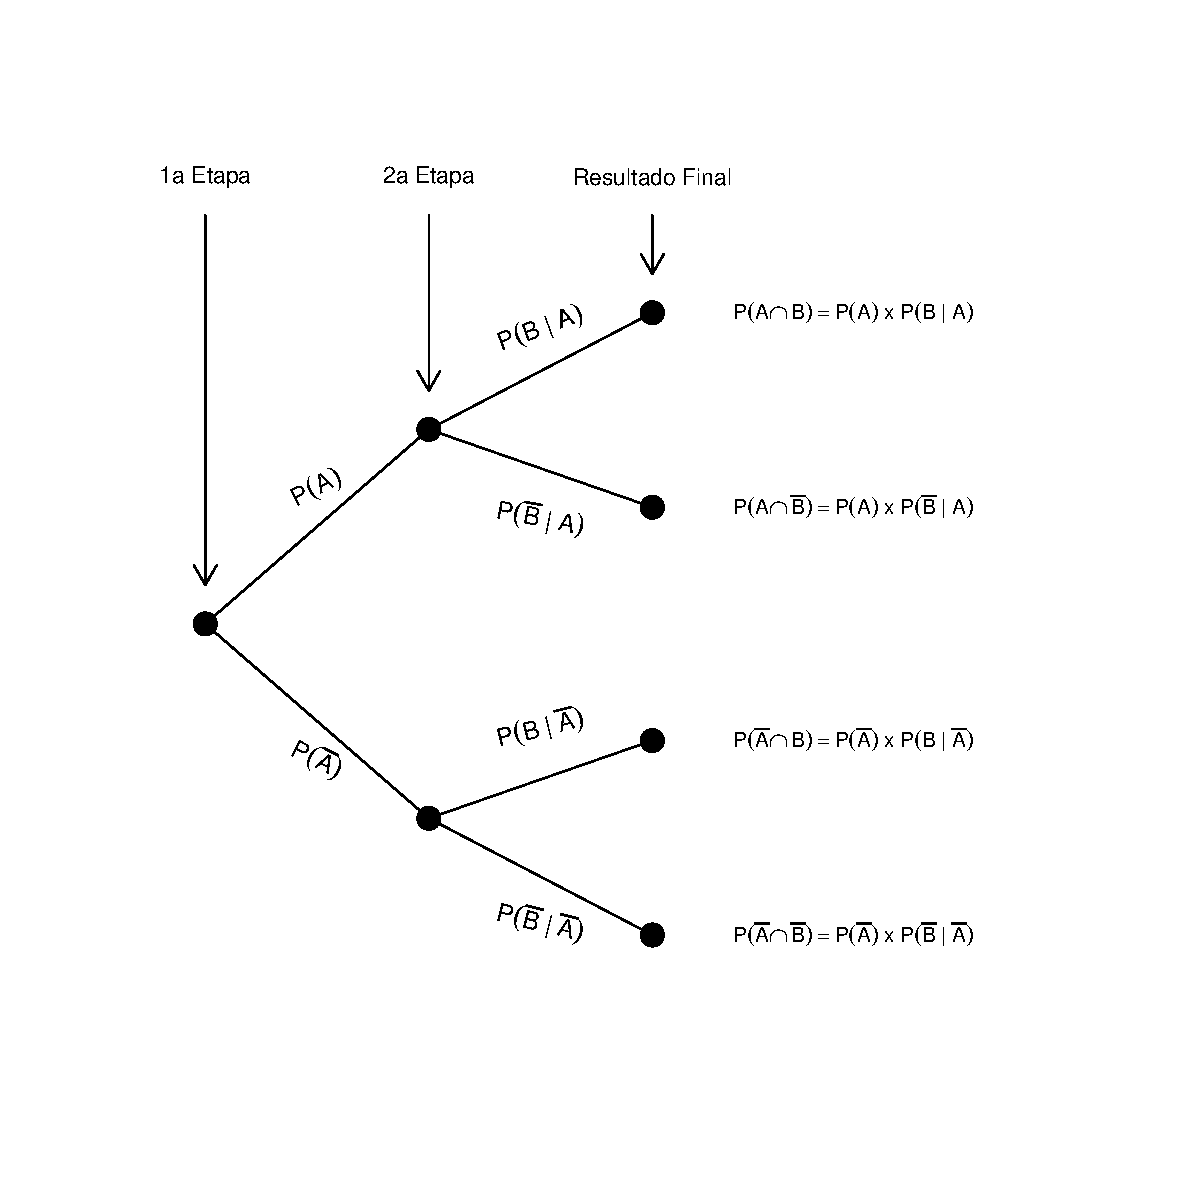
\includegraphics{probest-cambientais_files/figure-latex/unnamed-chunk-95-1.pdf}

\textbf{ii. O valor de \(b\)}

Se \(P(X \ge b) = 0,85\), a área abaixo de \(b\) que devemos encontrar na tabela \(Z\) é \(1 - 0,85 = 0.15\). Vemos que o valor mais próximo é \(0,1492\) que corresponde a \(z = -1,04\). Ao utilizar este resultado na expressão abaixo temos:

\(z = \frac{b - \mu}{\sigma} :: -1,04 = \frac{b - 50}{10}\)

\(b = (-1,04 \times 10) + 50 = 39.6\)

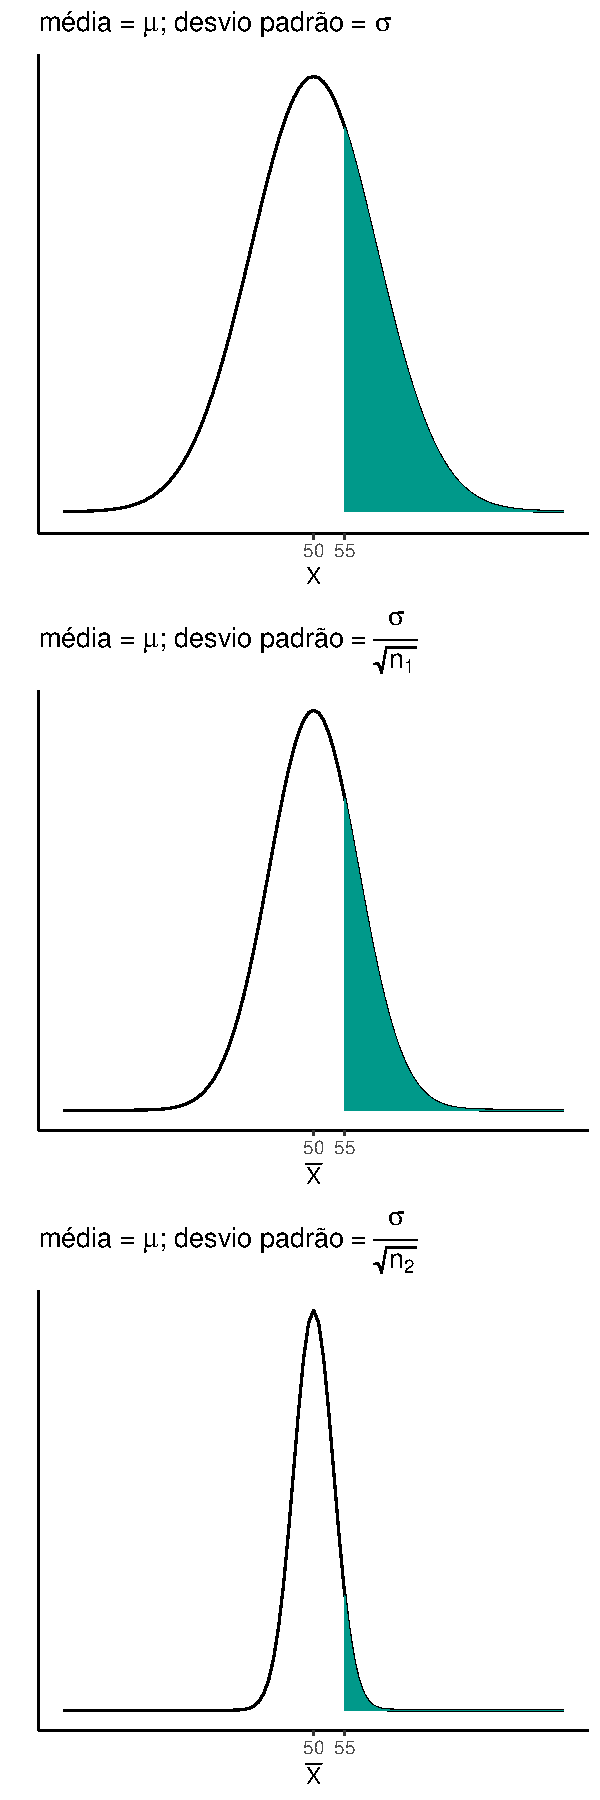
\includegraphics{probest-cambientais_files/figure-latex/unnamed-chunk-96-1.pdf}

\textbf{iii. O intervalo simétrico ao redor da média delimitado por \(c\) e \(d\) (\(c < d\)), que contém \(95\%\) da área sob a curva.}

Se entre \(c\) e \(d\) está \(95\%\) da área da curva, temos uma área de \(1 - 0,95 = 0,05\) fora da curva. Como o intervalo é simétrico, teremos \(0,025\) abaixo de \(c\) e \(0,025\) acima de \(d\).

Ao procurar na tabela \(Z\) por \(0,025\) encontraremos \(z = -1,96\) que equivale ena distribuição de X a:

\(z = \frac{c - \mu}{\sigma} :: -1,96 = \frac{c - 50}{10}\)

\(c = (-1,96 \times 10) + 50 = 30.4\)

Novamente, como o intervalo é simétrico e a dsitribuição de \(Z\) é centrada em zero, o ponto \(d\) será de +\(1,96\) que resulta em:

\(z = \frac{d - \mu}{\sigma} :: +1,96 = \frac{d - 50}{10}\)

\(d = (+1,96 \times 10) + 50 = 69.6\)

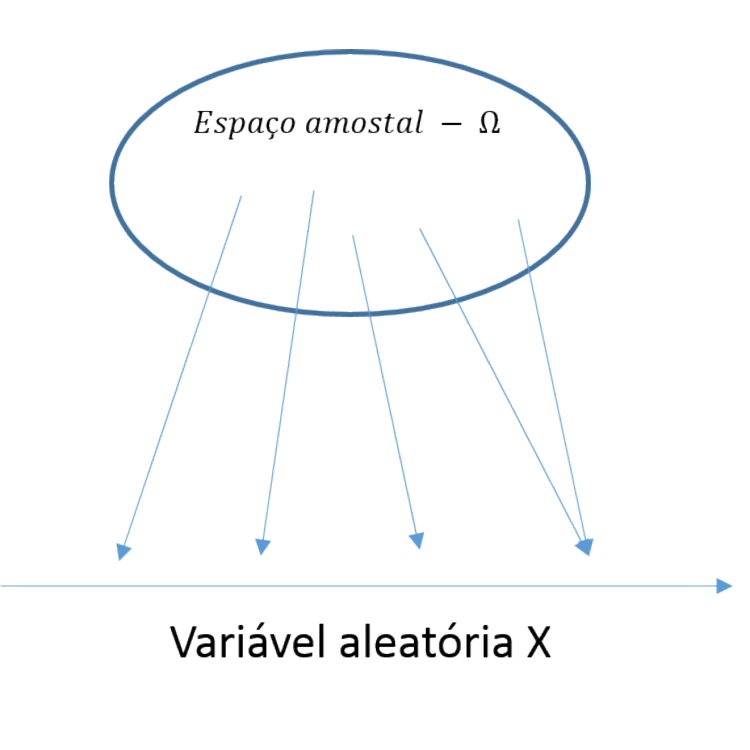
\includegraphics{probest-cambientais_files/figure-latex/unnamed-chunk-97-1.pdf}

\textbf{iv. O valor de \(e\) tal que \(P(50-e \le X \le 50+e) = 0.99\)}

Podemos fazer aqui:

\(P(50-e \le X \le 50+e) = P(\frac{50-e - \mu}{\sigma} \le \frac{X-\mu}{\sigma} \le \frac{50+e-\mu}{\sigma}) = 0.99\)

como \(\mu = 50\) e \(\sigma = 10\) temos:

\(P(\frac{-e}{10} \le Z \le \frac{e}{10}) = 0.90\)

Como a área central ocupa \(0,99\) da distribuição, restam \(0,005\) na cauda \textbf{superior} e \(0,005\) na cauda \textbf{inferior}:

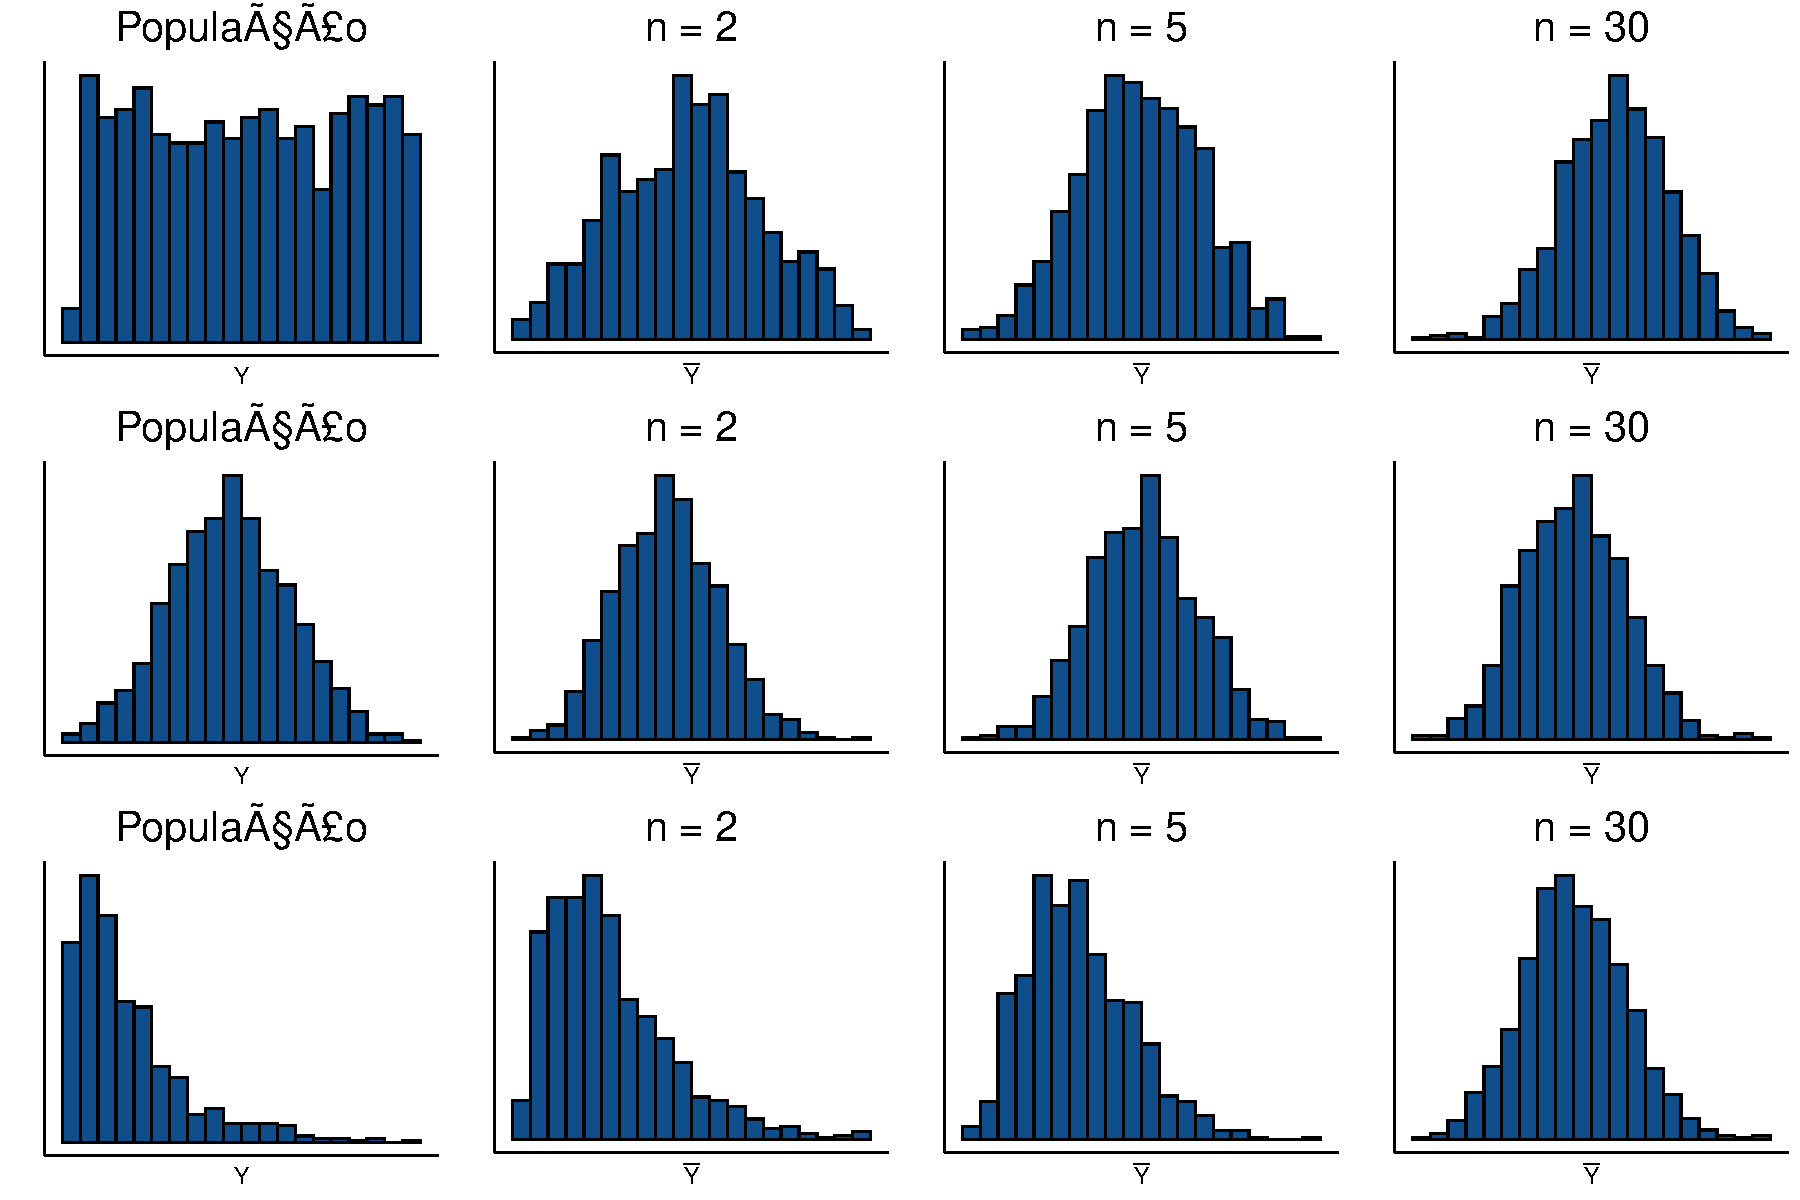
\includegraphics{probest-cambientais_files/figure-latex/unnamed-chunk-98-1.pdf}

Para encontrar \(-e\) buscamos por \(0,005\) na tabela \(Z\) e encontramos \(0,0051\) como valor mais próximo, referente a \(z_{-e} = -2,57\). Substituindo na equação temos:

\(\frac{-e}{10} \le -2,57 :: -e = -2,57 \times 10 :: e = 25,7\)

*Note na figura acima que os limite das áreas em azul são:

\(\mu - e = 50 - 25.7 = 24.3\) e

\(\mu - e = 50 + 25.7 = 75.7\)

\begin{center}\rule{0.5\linewidth}{0.5pt}\end{center}

O exercício pode ser resolvido pelo R por meio da função \texttt{qnorm}.

\begin{quote}
Em \texttt{qnorm}, o `q' vem de \emph{quantis} da distribuição normal.
\end{quote}

\begin{Shaded}
\begin{Highlighting}[]
\NormalTok{mu }\OtherTok{=} \DecValTok{50}
\NormalTok{sigma }\OtherTok{=} \DecValTok{10}

\NormalTok{(a }\OtherTok{\textless{}{-}} \FunctionTok{qnorm}\NormalTok{(}\AttributeTok{p =} \FloatTok{0.10}\NormalTok{, }\AttributeTok{mean =}\NormalTok{ mu, }\AttributeTok{sd =}\NormalTok{ sigma, }\AttributeTok{lower.tail =} \ConstantTok{TRUE}\NormalTok{))}
\end{Highlighting}
\end{Shaded}

\begin{verbatim}
## [1] 37.18448
\end{verbatim}

\begin{Shaded}
\begin{Highlighting}[]
\NormalTok{(b }\OtherTok{\textless{}{-}} \FunctionTok{qnorm}\NormalTok{(}\AttributeTok{p =} \DecValTok{1}\FloatTok{{-}0.85}\NormalTok{, }\AttributeTok{mean =}\NormalTok{ mu, }\AttributeTok{sd =}\NormalTok{ sigma, }\AttributeTok{lower.tail =} \ConstantTok{TRUE}\NormalTok{))}
\end{Highlighting}
\end{Shaded}

\begin{verbatim}
## [1] 39.63567
\end{verbatim}

\begin{Shaded}
\begin{Highlighting}[]
\NormalTok{(c }\OtherTok{\textless{}{-}} \FunctionTok{qnorm}\NormalTok{(}\AttributeTok{p =}\NormalTok{ (}\DecValTok{1}\FloatTok{{-}0.95}\NormalTok{)}\SpecialCharTok{/}\DecValTok{2}\NormalTok{, }\AttributeTok{mean =}\NormalTok{ mu, }\AttributeTok{sd =}\NormalTok{ sigma, }\AttributeTok{lower.tail =} \ConstantTok{TRUE}\NormalTok{))}
\end{Highlighting}
\end{Shaded}

\begin{verbatim}
## [1] 30.40036
\end{verbatim}

\begin{Shaded}
\begin{Highlighting}[]
\NormalTok{(d }\OtherTok{\textless{}{-}} \FunctionTok{qnorm}\NormalTok{(}\AttributeTok{p =}\NormalTok{ (}\DecValTok{1}\FloatTok{{-}0.95}\NormalTok{)}\SpecialCharTok{/}\DecValTok{2}\NormalTok{, }\AttributeTok{mean =}\NormalTok{ mu, }\AttributeTok{sd =}\NormalTok{ sigma, }\AttributeTok{lower.tail =} \ConstantTok{FALSE}\NormalTok{))}
\end{Highlighting}
\end{Shaded}

\begin{verbatim}
## [1] 69.59964
\end{verbatim}

\begin{Shaded}
\begin{Highlighting}[]
\NormalTok{(e }\OtherTok{\textless{}{-}} \SpecialCharTok{{-}}\FunctionTok{qnorm}\NormalTok{(}\AttributeTok{p =}\NormalTok{ (}\DecValTok{1}\FloatTok{{-}0.99}\NormalTok{)}\SpecialCharTok{/}\DecValTok{2}\NormalTok{, }\AttributeTok{mean =}\NormalTok{ mu, }\AttributeTok{sd =}\NormalTok{ sigma, }\AttributeTok{lower.tail =} \ConstantTok{TRUE}\NormalTok{) }\SpecialCharTok{+} \DecValTok{50}\NormalTok{)}
\end{Highlighting}
\end{Shaded}

\begin{verbatim}
## [1] 25.75829
\end{verbatim}

\hypertarget{quantos-desvios-padruxf5es}{%
\subsection{Quantos desvios padrões?}\label{quantos-desvios-padruxf5es}}

Suponha uma variável aleatória normalmente distribuída representada por \(X \sim \mathcal{N}(\mu,\,\sigma^2)\), determine:

\begin{enumerate}
\def\labelenumi{\roman{enumi}.}
\tightlist
\item
  O valor de \(a\) tal que \(P(X < a) = 0,20\).
\item
  \(P(X \le \mu + 2\sigma)\).
\item
  O valor de \(c\) tal que \(P(\mu -c\sigma \le X \le \mu +c\sigma) = 0.99\)
\end{enumerate}

\textbf{RESOLUÇÃO}

\textbf{i. O valor de \(a\) tal que \(P(X < a) = 0,20\).}

\(P(X < a) = P(\frac{X - \mu}{\sigma} < \frac{a - \mu}{\sigma}) = P(Z < \frac{a - \mu}{\sigma}) = 0,20\)

Procurando pelo valor de \(z\) que delimita \(0,20\) da área abaixo de \(a\) encontramos por \(z = -0,84\), de modo que:

\(-0,84 = \frac{a - \mu}{\sigma}\)

\(a = \mu -0,84\sigma\)

\textbf{ii. \(P(X \le \mu + 2\sigma)\)}

A expressão \(\mu + 2\sigma\) nos diz que o limite de interesse está \(2\) desvios padrões \textbf{acima} de \(\mu\). Ao procurar pelo valor de \(z = 2,0\) na tabela \(Z\), veremos que a probabilidade de interesse é \(P(X \le \mu + 2\sigma) = 0,9772\)

\textbf{iii. O valor de \(c\) tal que \(P(\mu -c\sigma \le X \le \mu +c\sigma) = 0.99\)}

Desenvolvendo esta expressão teremos

\(P(-c \le \frac{X - \mu}{\sigma} \le +c) = P(-c \le Z \le +c) = 0.99\)

Fora deste intervalo simétrico, teremos uma área de \(0,005\) na cauda inferior e \(0,005\) na cauda superior da distribuição \(Z\).

Ao procurar por \(0,005\) na tabela \(Z\) encontramos \(z = -2,57\), de modo que \(c = 2,57\).

\hypertarget{exercuxedcios-propostos}{%
\section{Exercícios propostos}\label{exercuxedcios-propostos}}

Leia o tópico \textbf{7.4.2 O Modelo Normal} em \citep{bussabemoretin6a} (pag. 176 a 181) e faça os exercícios 14 a 20 da página 184.

\hypertarget{tcl}{%
\chapter{Distribuição das médias amostrais}\label{tcl}}

Vamos retomar algumas ideias discutidas nos capítulos \ref{posicao} e \ref{amostrmedias}, quando apresentamos a distribuição das médias amostrais e o ciclo de \emph{amostragem} \(\Rightarrow\) \emph{inferência estatística}. Ao amostrar uma população estatística por meio de um experimento, seremos capazes de calcular estatísticas descritivas desta população. A média amostral \(\overline{X}\) é uma destas estimativas, mas a mesma ideia vale para \textbf{qualquer outra estatística \(\theta\)}.

\begin{figure}

{\centering 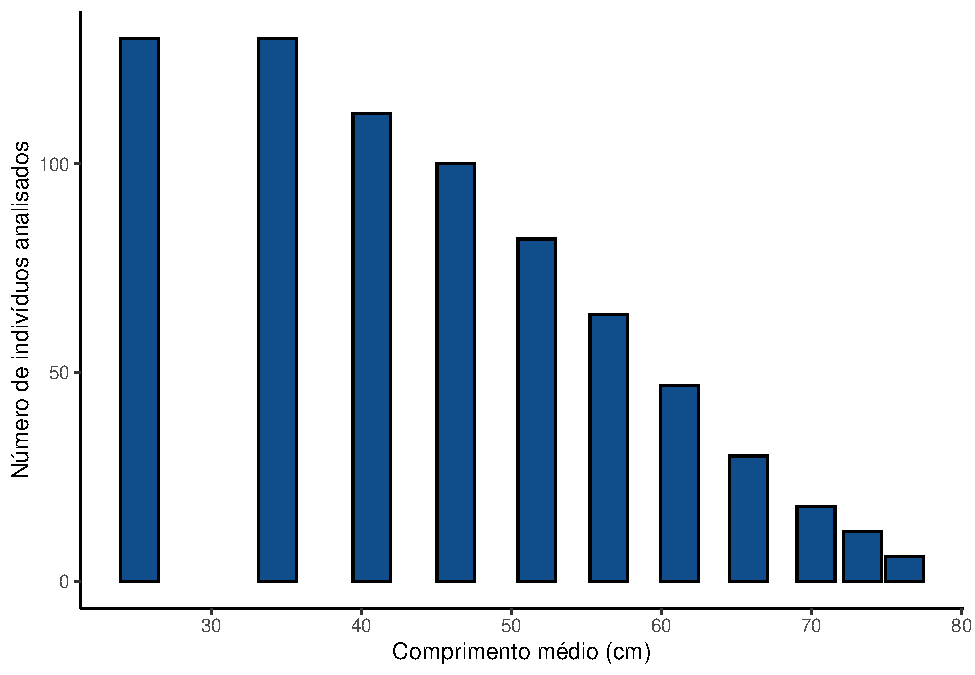
\includegraphics[width=20.83in]{probest-cambientais_files/figure-latex/unnamed-chunk-102-1} 

}

\caption{Processo de amostragem e inferência estatística}\label{fig:unnamed-chunk-102}
\end{figure}

Neste processo, o resultado de um experimento pode ser visto como uma observação particular de uma \textbf{população de experimentos} que podem ser reproduzidos sob as mesmas condições. A estimativa obtida deste experimento é portanto, somente uma entre uma \textbf{população de estimativas} que o experimento pode gerar. A inferência estatística é possível se pudermos entender o que é esperado como resultados desta população de experimentos.

\begin{figure}

{\centering 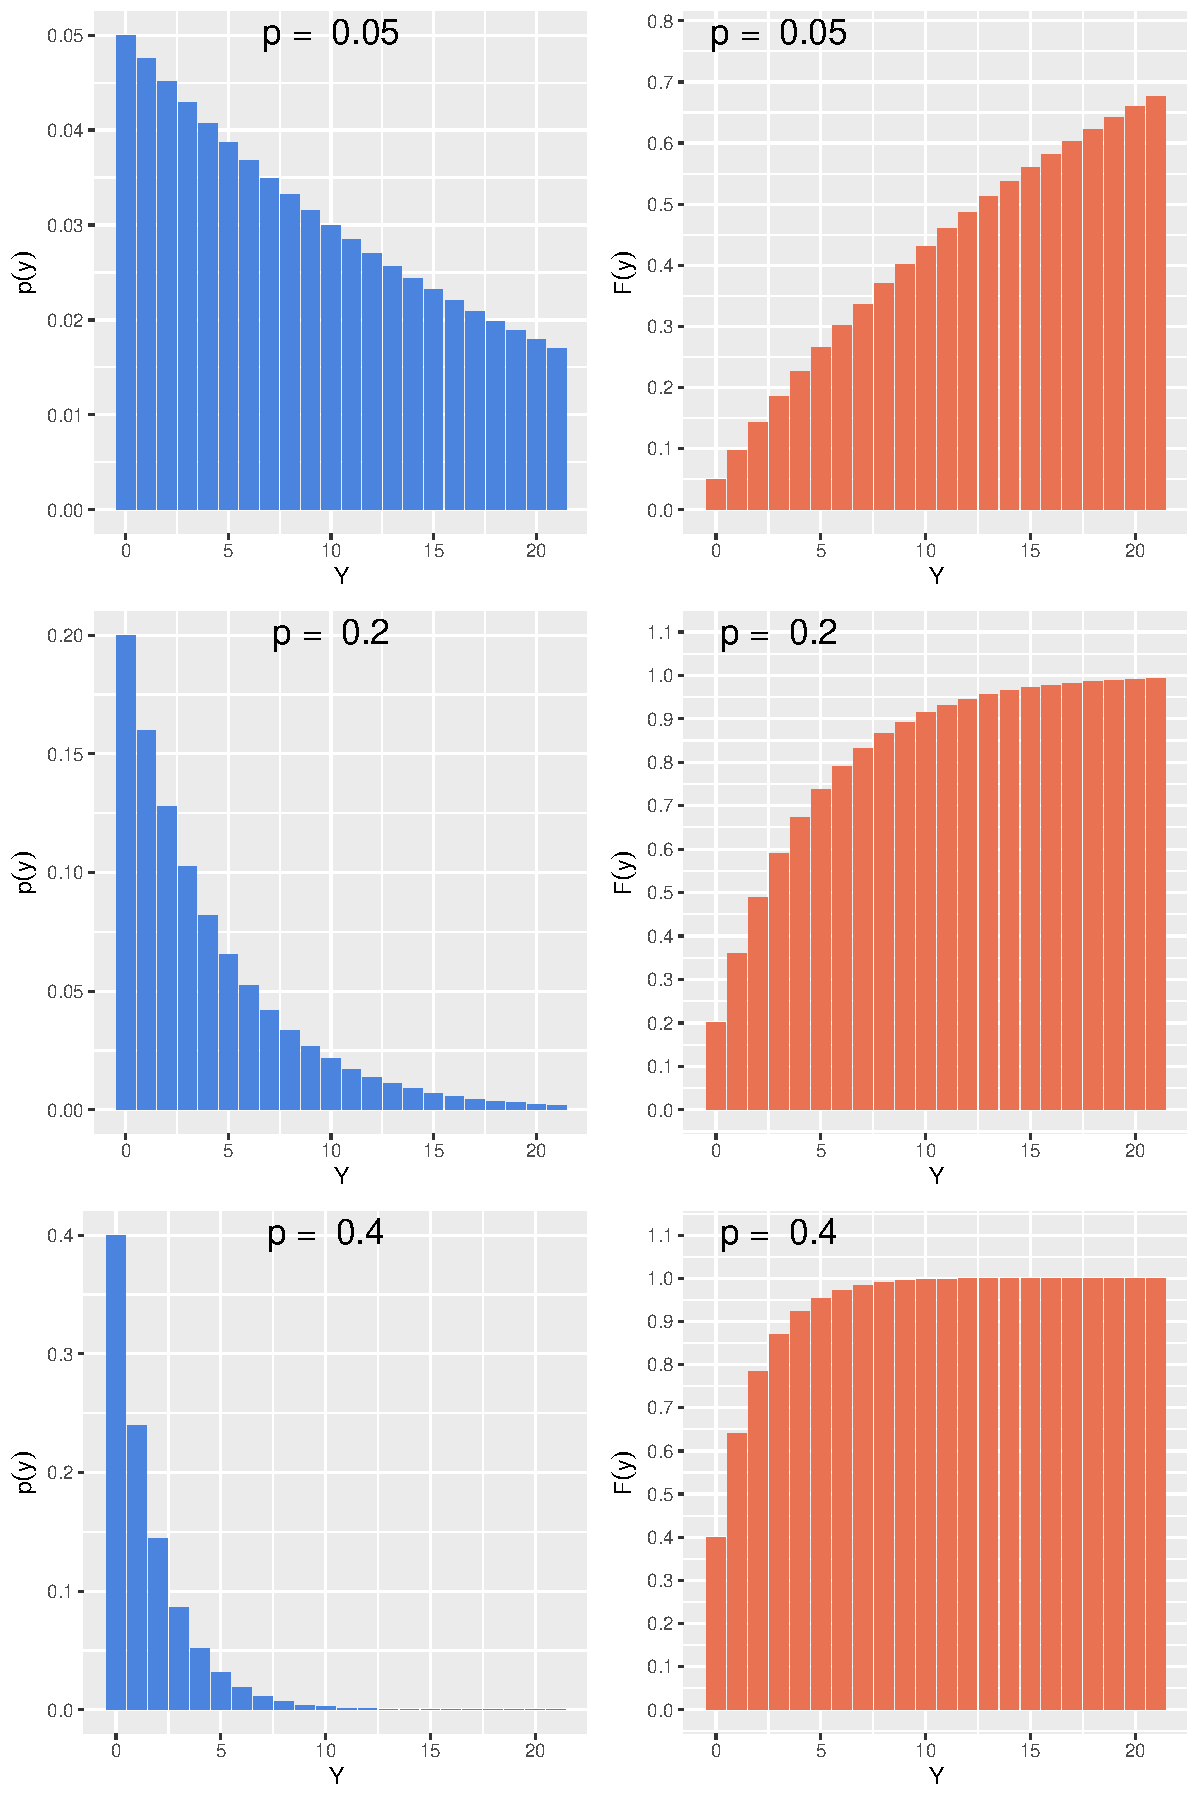
\includegraphics[width=20.83in]{probest-cambientais_files/figure-latex/unnamed-chunk-103-1} 

}

\caption{Distribuição das médias amostrais provinientes de um experimento}\label{fig:unnamed-chunk-103}
\end{figure}

\hypertarget{teorema-central-do-limite}{%
\section{Teorema Central do Limite}\label{teorema-central-do-limite}}

No capítulo \ref{amostrmedias} apresentamos a distribuição de médias como uma distribuição normal, centrada na média populacional \(\mu\) e com desvio padrão igual a \(\sigma_{\mu} = \frac{\sigma}{\sqrt{n}}\). Este resultado é previsto pelo \textbf{Teorema Central do Limite (TCL)} que fornece um \textbf{modelo teórico} para o comportamento esperado da média amostral de um experimento.

\begin{quote}
DEFINIÇÃO DO TCL: Seja uma popuilação estatística com média \(\mu\) e desvio padrão \(\sigma\). A distribuição das médias amostrais desta população tenderá a apresentar uma distribuição normal de probabilidades com média \(\mu\) e desvio padrão \(\frac{\sigma}{\sqrt(n)}\) à medida que o tamanho amostral \(n\) aumenta, ainda que a dsitribuição das observações originais \textbf{não possua} uma distribuição normal.
\end{quote}

Segundo o TCL, as médias amostrais \(\overline{X}\) de um experimento distribuem-se como:

\[\overline{X} \sim \mathcal{N}(\mu_{\overline{X}},\,\sigma^{2}_{\overline{X}})\]

em que \(\mu_{\overline{X}} = \mu\) \(\sigma^{2}_{\overline{X}} = \frac{\sigma^2}{n}\)

Note que a variância de \(\overline{X}\) depende do tamanho amostral \(n\). Isto justifica o que será discutido no tópico \textbf{Introdução à suficiência amostral} do capítulo \ref{inferenc}.

\hypertarget{probabilidades-na-amostra-original-e-na-distribuiuxe7uxe3o-de-muxe9dias}{%
\subsection{Probabilidades na amostra original e na distribuição de médias}\label{probabilidades-na-amostra-original-e-na-distribuiuxe7uxe3o-de-muxe9dias}}

Seja uma variável \(X\) qualquer com \(\mu = 50\) e \(\sigma = 10\). As figuras abaixo comparam as probabilidades acima de \(x_1 = 55\) para as observações originais e para as distribuições de médias amostrais de tamanho \(n_1 = 2\) e \(n_2 = 10\).

\begin{center}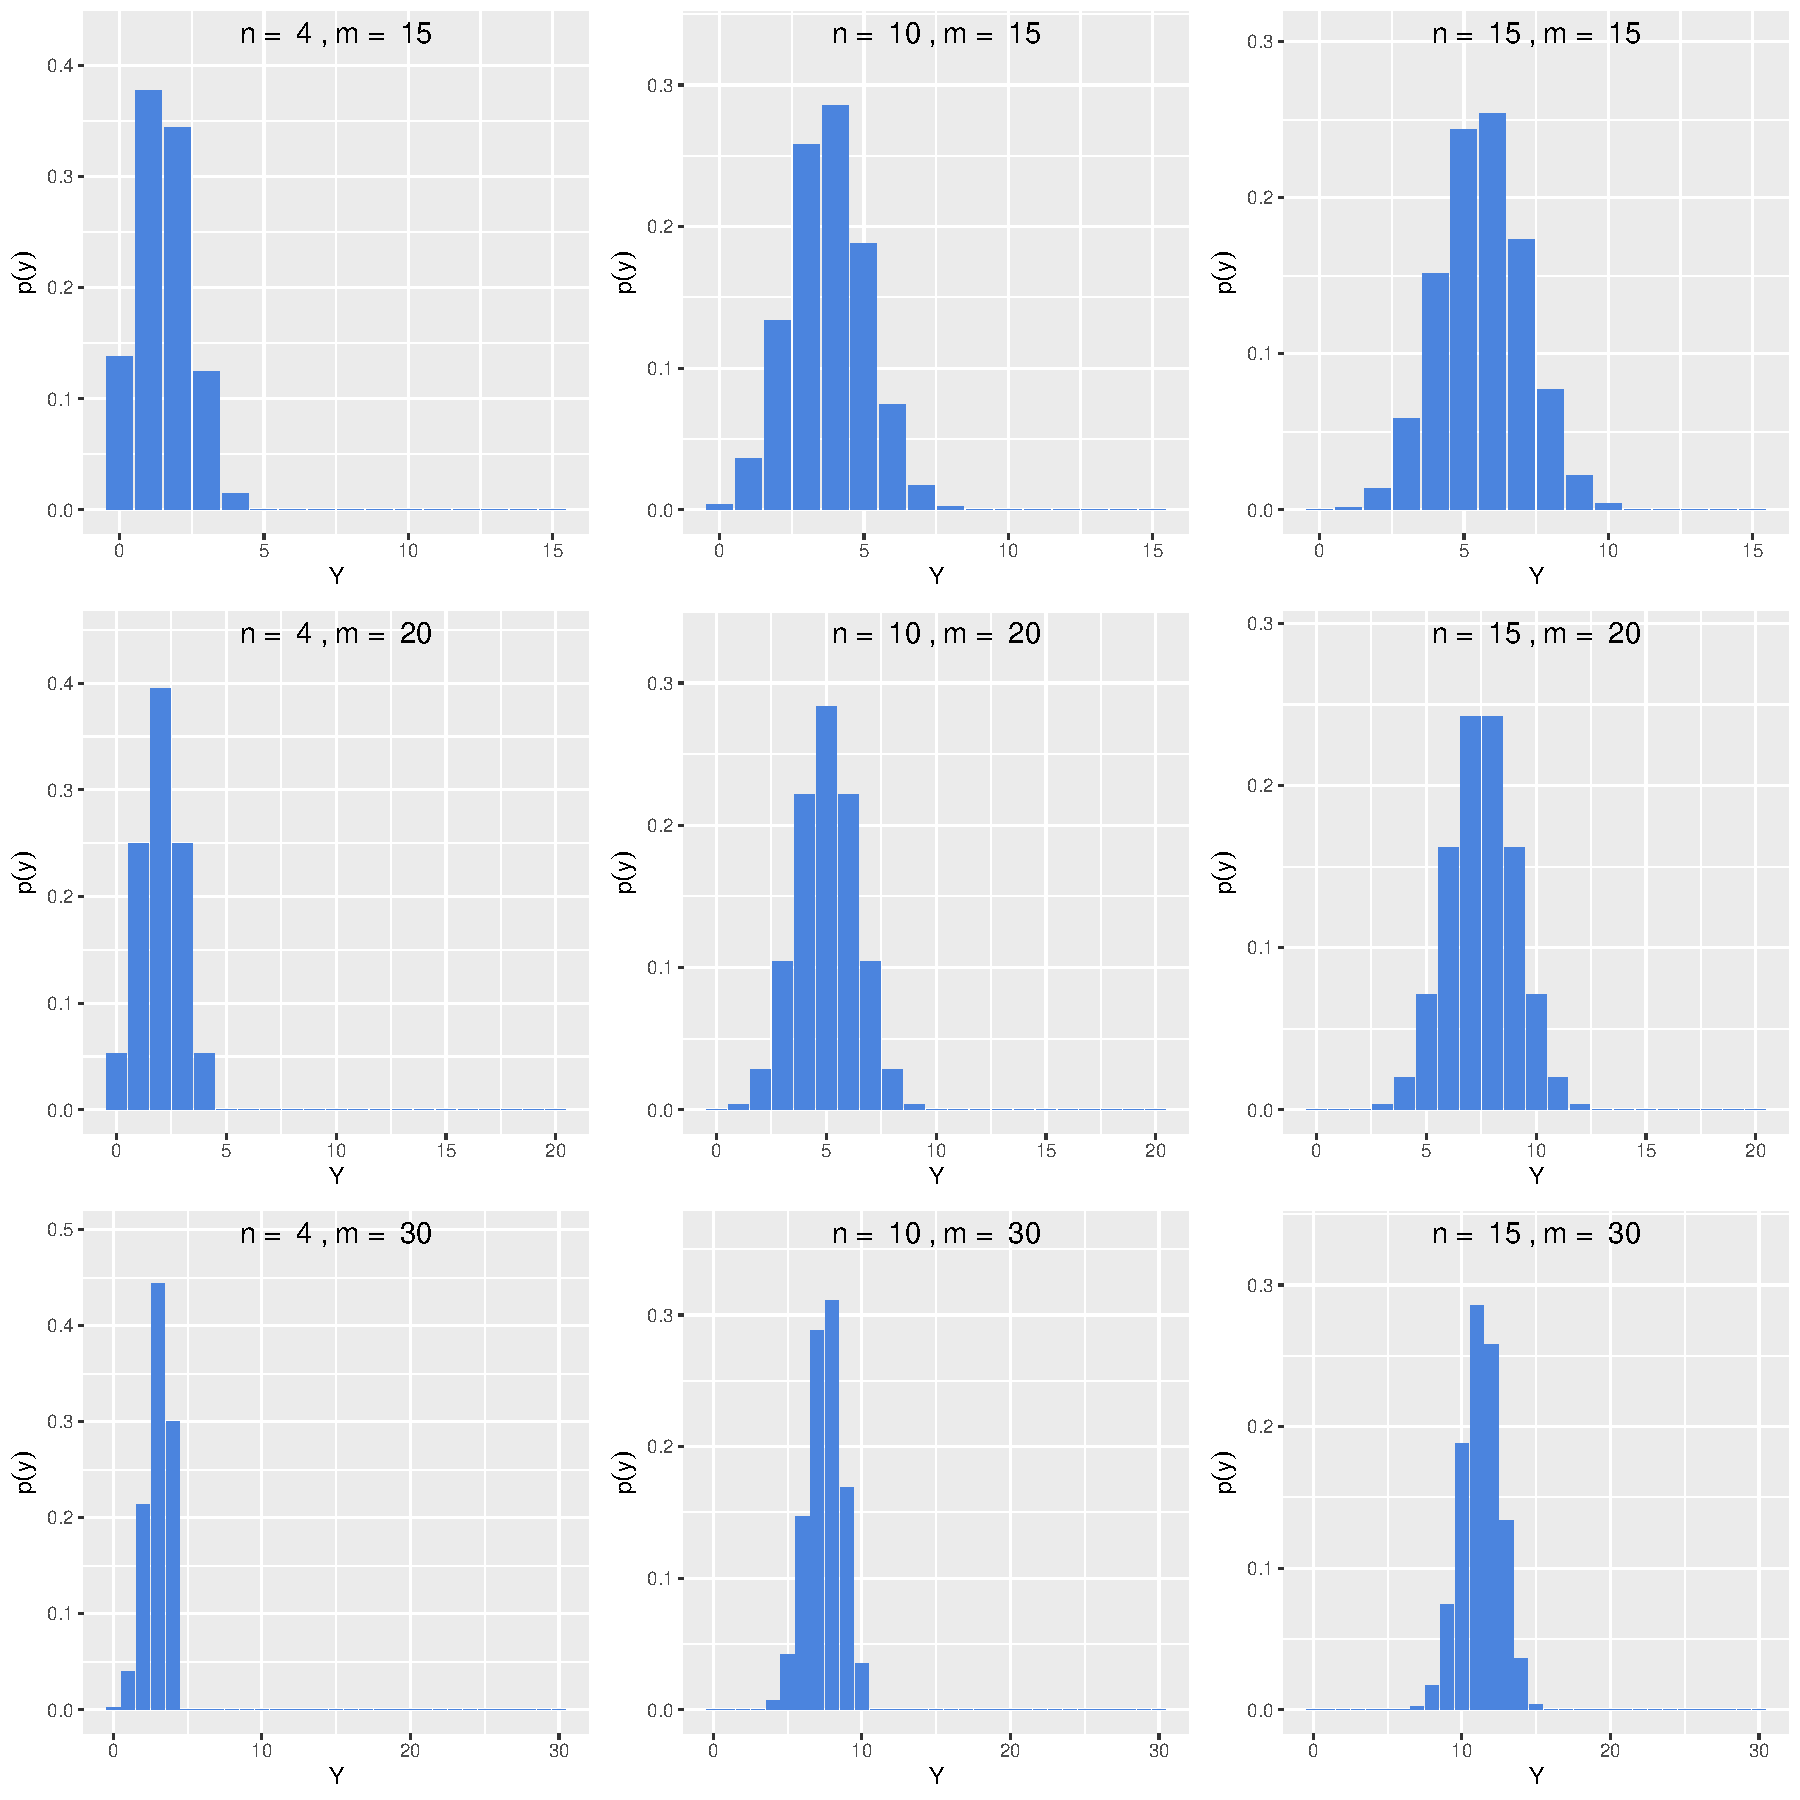
\includegraphics{probest-cambientais_files/figure-latex/unnamed-chunk-105-1} \end{center}

Note que existe uma probabilidade razoável de que uma determinada observação em \(X\) esteja acima de \(55\), \(P(X \leq 55) = 0.309\). No entando se tomarmos \emph{ao acaso} uma amostra de tamanho \(n_1 = 2\), a probabilidade de que \textbf{a média} destas duas amostras esteja acima de \(55\) diminui para \(P(\overline{X} \leq 55) = 0.24\). Se tormarmos uma amostra ainda maior (\(n_2 = 10\)), a probabilidade se reduz ainda mais para \(P(\overline{X} \leq 55) = 0.057\).

Vemos portanto, como mencionado no capítulo \ref{amostrmedias}, que a precisão de um experimento aumenta à medida que aumentamos o tamanho amostral, pois para amostras grandes, a probabilidade de obtermos um \(\overline{X}\) distante de \(\mu\) torna-se cada vez menor.

\hypertarget{distribuiuxe7uxe3o-nuxe3o-normais}{%
\subsection{Distribuição não-normais}\label{distribuiuxe7uxe3o-nuxe3o-normais}}

O TCL é válido inclusive para distribuições não-normais. Isto torna a distribuição normal uma das mais importantes em inferência estatística, pois ainda que o resultado de um experimento particular seja descrito por \emph{qualquer outro modelo de probabilidades}, as \textbf{médias das amostras} deste experimento seguirão uma distribuição normal, à medida que \(n\) aumenta. Isto justifica muitos dos processos de análise e inferência estatística que serão descritos nos capítulos posteriores.

A figura abaixo por exemplo, simula a distribuição de médias amostrais para variáveis com diferentes distribuições de probabiidades e tamanhos crescentes de \(n\). Podemos observar que \emph{independente} do formato da distribuição original, a distribuição das médias amostrais \emph{tende à normalidade}. O padrão normal aparece mais rápido se a distribuição original é \textbf{simétrica}. Por outro lado, para populações estatísticas com distribuições \textbf{assimétricas}, será necessário um tamanho amostral maior para que se alcance a normalidade.

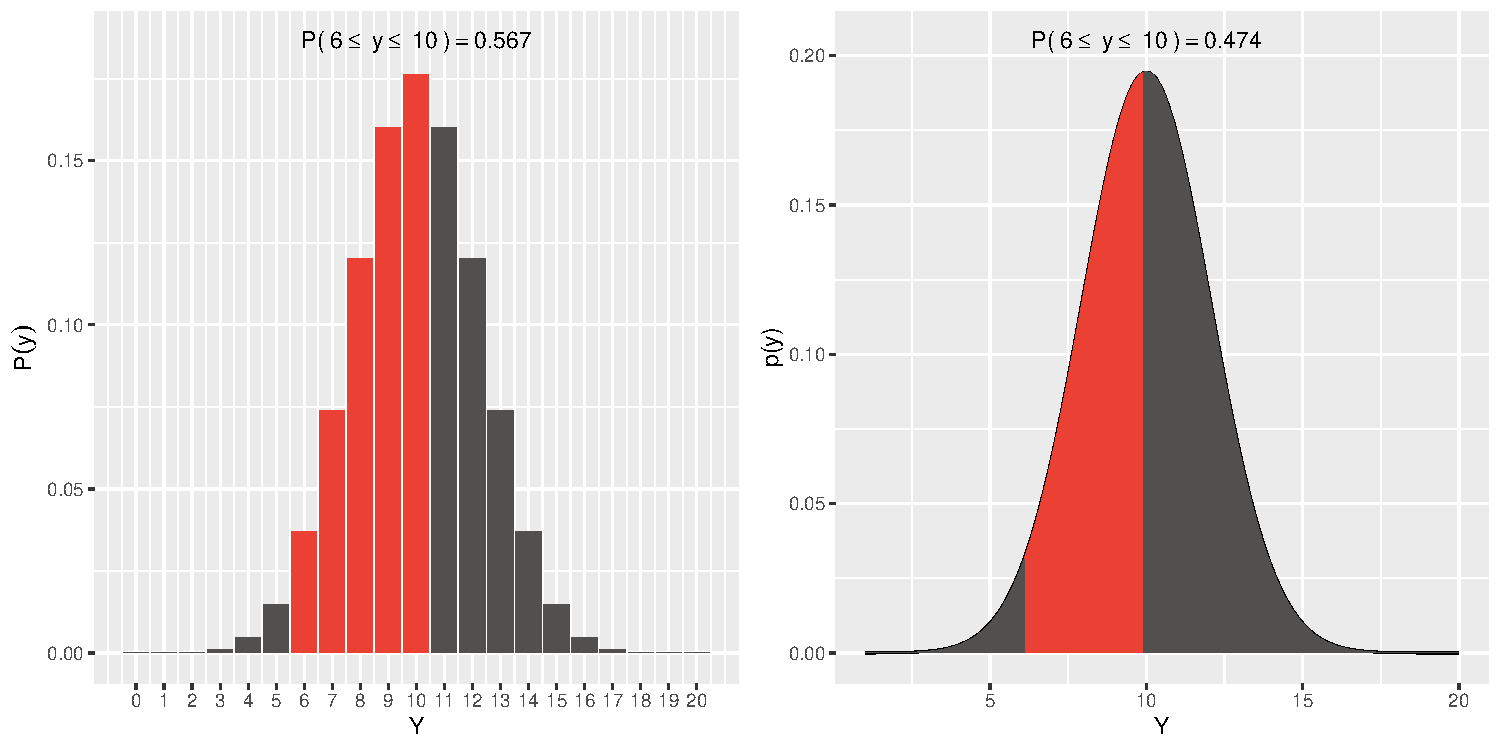
\includegraphics{probest-cambientais_files/figure-latex/unnamed-chunk-107-1.pdf}

\hypertarget{exercuxedcios-resolvidos-1}{%
\section{Exercícios resolvidos:}\label{exercuxedcios-resolvidos-1}}

\hypertarget{tamanho-muxe9dio-de-robalos-no-mercado-de-peixes}{%
\subsection{Tamanho médio de robalos no mercado de peixes}\label{tamanho-muxe9dio-de-robalos-no-mercado-de-peixes}}

Em 2014 no estuário do rio Itanhaém - SP foi pescado o \emph{``maior robalo já encontrado''} \href{http://g1.globo.com/sp/santos-regiao/noticia/2014/11/pescador-fisga-em-itanhaem-o-maior-robalo-ja-encontrado-briguei-com-ele.html}{(G1 Santos)}. O peixe tinha \(133\) cm e \(27,8\) kg . Em 2018 em Bertioga, também no litoral de SP \emph{``Robalo `gigante' quebra recordes e vira atração''} \href{https://g1.globo.com/sp/santos-regiao/noticia/robalo-gigante-quebra-recordes-e-vira-atracao-durante-pescaria-em-sp.ghtml}{(G1 Santos)} pesando \(33\) kg. Em ``\emph{uma das salas da Colônia de Pesca Z2 de Atafona}'' RJ está uma imagem de um robalo de \(28\) kg capturado muitas décadas atrás \href{http://ambientecult.blogspot.com/2010/10/ponto-de-memoria-foto-da-pesca.html}{(Ambiente Cult)}.

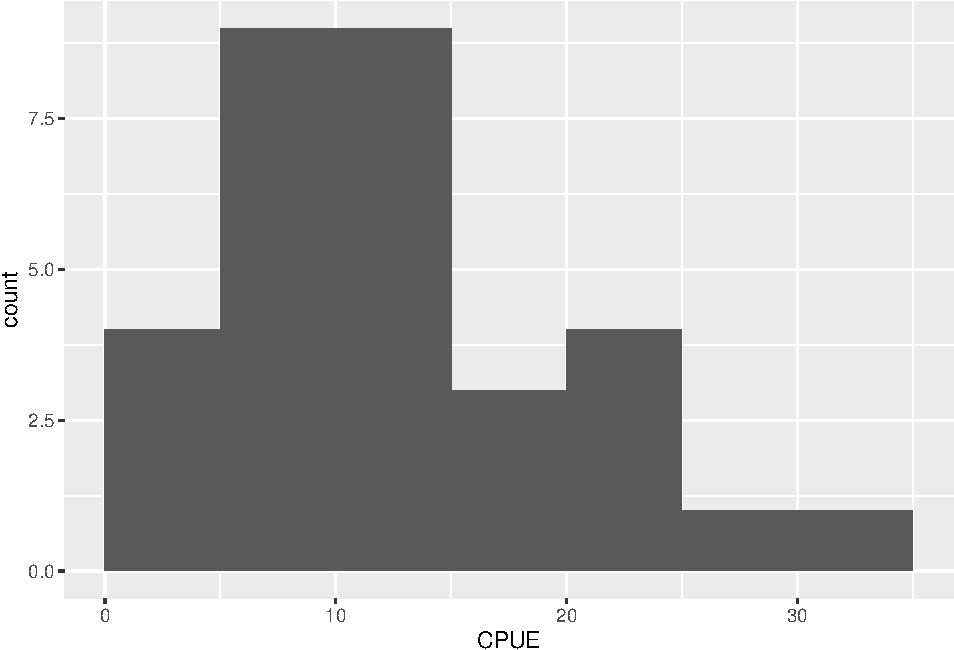
\includegraphics[width=20.83in]{probest-cambientais_files/figure-latex/unnamed-chunk-109-1}

Estas capturas viram notícias pois são certamente inusitadas. Dados de desembarque sugerem que a distribuição de tamanho de robalos comumente capturados está muito abaixo destes limites \citep{ximanes-carvalo2006} ( \href{http://repositorio.ufc.br/bitstream/riufc/1312/1/2006_dis_moxcarvalho.pdf}{Acesse aqui o trabalho completo} ).

\begin{figure}
\centering
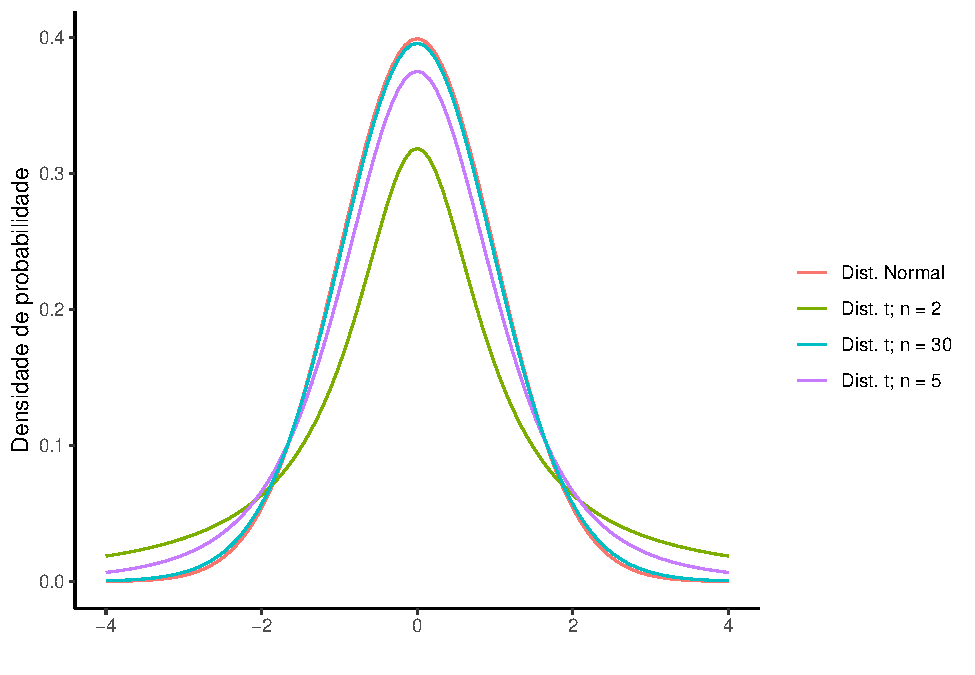
\includegraphics{probest-cambientais_files/figure-latex/unnamed-chunk-111-1.pdf}
\caption{\label{fig:unnamed-chunk-111}Dados de desembarque no Mercado de São Pedro (Niterói, RJ). Extraídos de XIMENES-CARVALHO, 2006.}
\end{figure}

Esta distribuição é altamente assimétrica e claramente \textbf{não-normal}. Um dos motivos para este forte grau de assimetria deve-se ao limite inferior de captura. A captura e comercialização de animais muito pequenos é proibida. Suponha que o comprimento de robalos (\(L\)) disponíveis para compra tenha média \(\mu = 44.1\) e desvio padrão \(\sigma = 13.4\). Você compra 10 robalos escolhidos ao acaso dos que estão disponíveis. Qual a probabilidade de que:

\begin{enumerate}
\def\labelenumi{\roman{enumi}.}
\tightlist
\item
  O tamanho médio de uma compra esteja acima de \(52,4\) cm, isto é \(P(\overline{L} > 52,4)\)?
\item
  Em \(95\%\) das vezes que fizer a compra, determine o intervalo simétrico que conterá o tamanho médio dos robalos selecionados, isto é \(P(a \le \overline{L} \le b) = 0,95\)
\item
  Responda novamente aos itens i. e ii. no caso de sua compra constar de \(4\) robalos.
\end{enumerate}

\textbf{RESOLUÇÃO}

Ainda que a distribuição original claramente não siga uma distribuição normal, podemos utilizar o TCL para estimarmos as probabilidades de obter uma média amostral \(\overline{X}\) a determinada distância de \(\mu\). Para isto, no entanto devemos recordar que o desvio padrão das médias amostrais será dado por: \(\sigma_{\overline{X}} = \frac{\sigma}{\sqrt{n}}\).`

\textbf{i. \(P(\overline{L} > 52,4)\)}

Com base no TCL, uma amostra de \(n = 10\) terá média normalmente distribuída com parâmetros \(\mu\) e \(\sigma_{\mu} = \frac{\sigma}{\sqrt{10}}\). Podemos assim, realizar a transformação \(Z\) como segue:

\(Z_{\overline{L}} = \frac{\overline{L} - \mu}{\sigma_{\mu}} = \frac{\overline{L} - \mu}{\frac{\sigma}{\sqrt{n}}}\)

\(Z_{\overline{L}} = \frac{52,4 - 44.1}{\frac{13.4}{\sqrt{10}}} = 1.96\)

\begin{quote}
Note que o denomidador aqui é \emph{diferente} do que fizemos no capítulo \ref{normdist}, pois aqui estamos falando da distribuição das \textbf{médias amostrais} \(\overline{L}\) e não nas observações individuais \(L\).
\end{quote}

Se buscarmos na Tabela Z, veremos que a área da distribuição normal padronizada abaixo de \(1.96\) é de \(0,975\). Consequentemente \(P(\overline{L} > 52,4) = 1 - 0,975 = 0,025\)

\textbf{ii. \(P(a \le \overline{L} \le b) = 0,95\)}

Se o intervalo é simétrico e contém \(0,95\) das observações, restam \(0,025\) em cada uma das caudas. Vimos no item anterior que \(z = 1,96\) que delimita \(0,025\) da cauda superior. Portanto os limites aqui serão dados por: \(a = -1.96\) e \(b = 1.96\). Na distribuição original estes limites resultarão em:

\(-1,96 = \frac{a - 44.1}{\frac{13.4}{\sqrt{10}}}:: a = 44.1 -1,96 \frac{13.4}{\sqrt{10}} = 35.8\) cm

e

\(+1,96 = \frac{b - 44.1}{\frac{13.4}{\sqrt{10}}}:: b = 44.1 +1,96 \frac{13.4}{\sqrt{10}} = 52.4\) cm

\textbf{Responda novamente aos itens i. e ii. no caso de sua compra constar de \(4\) robalos.}

Aqui você deve repetir exatamente os passos de i. e ii. substituindo \(n = 10\) por \(n = 4\).

\begin{center}\rule{0.5\linewidth}{0.5pt}\end{center}

No R temos:

\textbf{i. \(P(\overline{L} > 52,4)\)}

\begin{Shaded}
\begin{Highlighting}[]
\FunctionTok{pnorm}\NormalTok{(}\FloatTok{52.4}\NormalTok{, }
      \AttributeTok{mean =} \FloatTok{44.1}\NormalTok{, }
      \AttributeTok{sd =} \FloatTok{13.4}\SpecialCharTok{/}\FunctionTok{sqrt}\NormalTok{(}\DecValTok{10}\NormalTok{), }
      \AttributeTok{lower.tail =} \ConstantTok{FALSE}\NormalTok{)}
\end{Highlighting}
\end{Shaded}

\begin{verbatim}
## [1] 0.02507255
\end{verbatim}

\textbf{ii. \(P(a \le \overline{L} \le b) = 0,95\)}

\begin{Shaded}
\begin{Highlighting}[]
\NormalTok{a }\OtherTok{\textless{}{-}} \FunctionTok{qnorm}\NormalTok{((}\DecValTok{1}\FloatTok{{-}0.95}\NormalTok{)}\SpecialCharTok{/}\DecValTok{2}\NormalTok{, }
      \AttributeTok{mean =} \FloatTok{44.1}\NormalTok{, }
      \AttributeTok{sd =} \FloatTok{13.4}\SpecialCharTok{/}\FunctionTok{sqrt}\NormalTok{(}\DecValTok{10}\NormalTok{), }
      \AttributeTok{lower.tail =} \ConstantTok{TRUE}\NormalTok{)}
\NormalTok{a}
\end{Highlighting}
\end{Shaded}

\begin{verbatim}
## [1] 35.79475
\end{verbatim}

\begin{Shaded}
\begin{Highlighting}[]
\NormalTok{b }\OtherTok{\textless{}{-}} \FunctionTok{qnorm}\NormalTok{((}\DecValTok{1}\FloatTok{{-}0.95}\NormalTok{)}\SpecialCharTok{/}\DecValTok{2}\NormalTok{, }
      \AttributeTok{mean =} \FloatTok{44.1}\NormalTok{, }
      \AttributeTok{sd =} \FloatTok{13.4}\SpecialCharTok{/}\FunctionTok{sqrt}\NormalTok{(}\DecValTok{10}\NormalTok{), }
      \AttributeTok{lower.tail =} \ConstantTok{FALSE}\NormalTok{)}
\NormalTok{b}
\end{Highlighting}
\end{Shaded}

\begin{verbatim}
## [1] 52.40525
\end{verbatim}

\textbf{iii. \(P(\overline{L} > 52,4)\) para \(n = 4\)}

\begin{Shaded}
\begin{Highlighting}[]
\FunctionTok{pnorm}\NormalTok{(}\FloatTok{52.4}\NormalTok{, }
      \AttributeTok{mean =} \FloatTok{44.1}\NormalTok{, }
      \AttributeTok{sd =} \FloatTok{13.4}\SpecialCharTok{/}\FunctionTok{sqrt}\NormalTok{(}\DecValTok{4}\NormalTok{), }
      \AttributeTok{lower.tail =} \ConstantTok{FALSE}\NormalTok{)}
\end{Highlighting}
\end{Shaded}

\begin{verbatim}
## [1] 0.1077087
\end{verbatim}

\textbf{ii. \(P(a \le \overline{L} \le b) = 0,95\) para \(n = 4\)}

\begin{Shaded}
\begin{Highlighting}[]
\NormalTok{a }\OtherTok{\textless{}{-}} \FunctionTok{qnorm}\NormalTok{((}\DecValTok{1}\FloatTok{{-}0.95}\NormalTok{)}\SpecialCharTok{/}\DecValTok{2}\NormalTok{, }
      \AttributeTok{mean =} \FloatTok{44.1}\NormalTok{, }
      \AttributeTok{sd =} \FloatTok{13.4}\SpecialCharTok{/}\FunctionTok{sqrt}\NormalTok{(}\DecValTok{4}\NormalTok{), }
      \AttributeTok{lower.tail =} \ConstantTok{TRUE}\NormalTok{)}
\NormalTok{a}
\end{Highlighting}
\end{Shaded}

\begin{verbatim}
## [1] 30.96824
\end{verbatim}

\begin{Shaded}
\begin{Highlighting}[]
\NormalTok{b }\OtherTok{\textless{}{-}} \FunctionTok{qnorm}\NormalTok{((}\DecValTok{1}\FloatTok{{-}0.95}\NormalTok{)}\SpecialCharTok{/}\DecValTok{2}\NormalTok{, }
      \AttributeTok{mean =} \FloatTok{44.1}\NormalTok{, }
      \AttributeTok{sd =} \FloatTok{13.4}\SpecialCharTok{/}\FunctionTok{sqrt}\NormalTok{(}\DecValTok{4}\NormalTok{), }
      \AttributeTok{lower.tail =} \ConstantTok{FALSE}\NormalTok{)}
\NormalTok{b}
\end{Highlighting}
\end{Shaded}

\begin{verbatim}
## [1] 57.23176
\end{verbatim}

\hypertarget{exercuxedcios-propostos-1}{%
\section{Exercícios propostos}\label{exercuxedcios-propostos-1}}

Leia dos tópicos \textbf{10.6 Estatísticas e Parâmetros} a \textbf{10.8 Distribuição Amostral da Média} em \citep{bussabemoretin6a} (pag. 271 a 281) e faça os exercícios 7 a 10 da página 281.

\hypertarget{inferenc}{%
\chapter{Inferindo sobre uma População Estatística}\label{inferenc}}

\hypertarget{estimauxe7uxe3o-pontual-e-estimauxe7uxe3o-intervalar}{%
\section{Estimação pontual e estimação intervalar}\label{estimauxe7uxe3o-pontual-e-estimauxe7uxe3o-intervalar}}

A média \(\overline{X}\) obtida a partir de uma determinada amostra varia em função das características das unidades amostrais que foram selecionadas (Capítulo \ref{amostrmedias}). Portanto, \(\overline{X}\) não será igual à média \(\mu\). No entanto, o TLC (Capítulo \ref{tcl}) nos garante que a distribuição esperada das médias amostrais terá uma distribuição normal e que a média das médias (\(\mu_{\overline{X}}\)) será igual a \(\mu\). Vimos ainda que o desvio padrão da distribuição das médias amostrais (conhecido como \textbf{erro padrão} - \(\sigma_{\overline{X}}\)) dependerá do tamanho da amostra \(n\), de acordo com a expressão:

\[\sigma_{\overline{X}} = \frac{\sigma}{\sqrt{n}}\]

Uma vez que não conhecemos \(\mu\), temos que \textbf{estimá-lo} a partir da amostra. Neste caso, \(\overline{X}\) será nossa \textbf{melhor estimativa} da média populacional. Dizemos que \(\overline{X}\) é o \textbf{estimador pontual} de \(\mu\).

Como \(\overline{X}\) varia em função de nossa amostra particular, devemos obter além da estimativa pontual, uma \textbf{estimativa intervalar} que nos é fornecida pelo \textbf{intervalo de confiança}.

\hypertarget{intervalo-de-confianuxe7a}{%
\subsection{Intervalo de confiança}\label{intervalo-de-confianuxe7a}}

\begin{quote}
DEFINIÇÃO: é um intervalo de valores associado a um determinado nível de significância (\(\alpha\)). Quando dizemos que um intervalo foi calculado a um nível de confiança de 95\% (\(1 - \alpha\)), estamos dizendo que a probabilidade dos limites do IC conterem o valor da média populacional \(\mu\) é de 95\%.
\end{quote}

O IC é calculado por:

\[IC_{1-\alpha} = \mu \pm z_{\alpha/2} \times \frac{\sigma}{\sqrt{n}}\]

O valor de \(z_{\alpha/2}\) é o valor do índice \(z\) associado ao nível de confiança desejado.

Se desejamos definir o intervalo de confiança a 95\% precisamos garantir que haja uma probabilidade de 95\% de que a média amostral esteja ao redor da média populacional. Deste modo, o limite deve excluir 2.5\% da porção superior e 2.5\% da porção inferior da curva. Para isto, definimos \(z_{\alpha/2} = 1.96\), sendo \(\alpha\) fixado em 0.05.

\begin{quote}
O valor \(z_{\alpha/2} = 1.96\) foi retirado da Tabela Z como o módulo do valor de \(z\) que delimida uma área inferior igual a \(0.025\).
\end{quote}

Se queremos um nível de confiança diferente, basta ajustar o valor de \(\alpha\). Por exemplo, se queremos um nível de significância a 99\%, fixamos \(\alpha\) em \(0.01\) e portanto \(z = 2.58\). Da mesma forma, o \(IC_{90\%}\) poderá ser obtido com \(\alpha = 0.10\) e consequentemente \(z = 1.64\). Estes e outros limites descrevem as probabilidades em uma distribuição normal padronizada (Capítulo \ref{normtlc}), que podem ser obtidos com o uso da maioria dos softwares estatísticos, além de estarem inclusos nas \textbf{Tabelas Z}, encontradas na grande maioria dos livros de estatística básica. Os valores de Z são os mesmos discutidos no tópico \textbf{Medidas de posição} quando discutimos os \textbf{Índice Z} (Capítulo \ref{posicao})

\begin{center}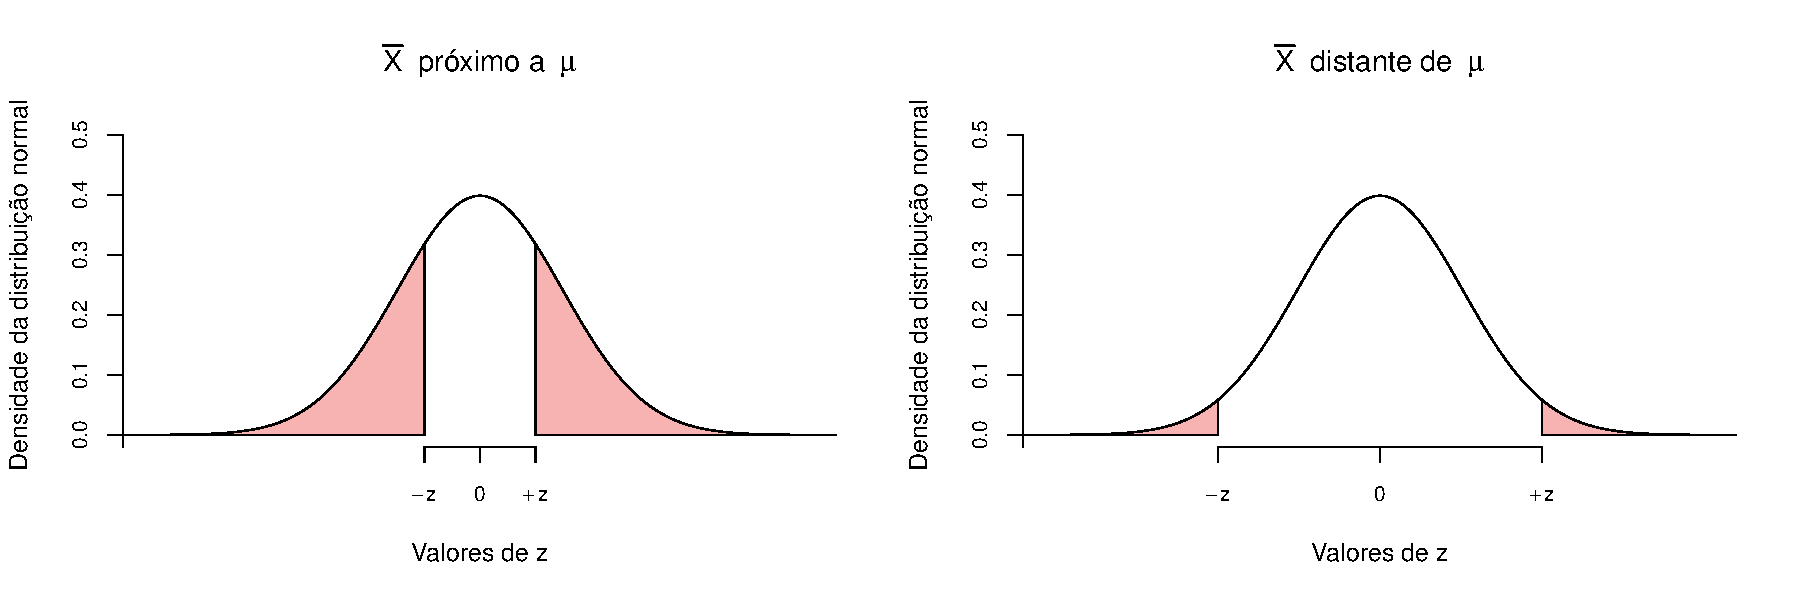
\includegraphics{probest-cambientais_files/figure-latex/unnamed-chunk-119-1} \end{center}

Para o cálculo do intervalo de confiança, estamos assumindo que as médias amostrais têm \textbf{Distribuição Normal} com média \(\mu\) e desvio padrão \(\frac{\sigma}{\sqrt{n}}\). Fazendo isto, estamos no \textbf{Teorema Central do Limite (TCL)} (Capítulo \ref{tcl}). Geralmente não temos os valores de \(\mu\) e \(\sigma\), de modo que utilizamos os valores de \(\overline{X}\) e \(s\) calculados a partir de nossa amostra. Quando as amostras são grandes (\(n\ge{30}\)) não há problema em utilizar o valor de \(z_{\alpha/2}\), e assim:

\[IC_{1-\alpha} = \overline{X} \pm z_{\alpha/2} \times \frac{s}{\sqrt{n}}\]

\hypertarget{distribuiuxe7ao-t-de-student}{%
\subsubsection{Distribuiçao t de Student}\label{distribuiuxe7ao-t-de-student}}

Quando não conhecemos \(\mu\) e \(\sigma\) e as amostras são pequenas (ex. \(n<30\)), a dsitribuiçao normal não é a melhor aproximação para o comportamento das médias amostrais. Nestes casos, substituímos a distribuição de \(z\) pela \textbf{Distribuição \(t\) de Student}, sendo o intervalo de confiança obtido por:

\[IC_{1-\alpha} = \overline{X} \pm t_{\alpha/2, gl} \times \frac{s}{\sqrt{n}}\]

Em que \(\alpha\) continua sendo o nível de significância e \(gl\) é definido como os \textbf{graus de liberdade}. Neste caso, os graus de liberdade são dados por:

\[gl = n-1\]

O formato da distribuição \(t\) de student não é constante. À medida que o tamanho amostral aumenta, o formado da distribuição \(t\) converge para a distribuição normal. Isto faz com que na prática \textbf{raremente} usaremos a distribuição de Z, substituindo-a pela distribuição \(t\) de Student.

\includegraphics{probest-cambientais_files/figure-latex/unnamed-chunk-120-1.pdf}

Para amostras pequenas (\(n = 2\)) o formato da distribuição de \(t\) é distinto da distribuição normal. No entanto, para tamanhos amostrais maiores (\(n = 30\)) as o formato da distribuição \(t\) tende a a convergir para o mesmo formato a distribuição normal. Esta característica implica que a área a partir de um determinado limite \(t_i\) não é constante como na distribuição normal, mas \emph{depende do tamanho da amostra}, como pode ser visto abaixo.

\begin{center}\includegraphics{probest-cambientais_files/figure-latex/unnamed-chunk-121-1} \end{center}

\hypertarget{introduuxe7uxe3o-uxe0-suficiuxeancia-amostral}{%
\section{Introdução à suficiência amostral}\label{introduuxe7uxe3o-uxe0-suficiuxeancia-amostral}}

Uma decisão central ao planejamento de um experimento é quanto recurso (ex. tempo, dinheiro, mão de obra) devem ser investidos para se obter \textbf{boas estimativas} dos parâmetros populacionais. Por boas estimativas, entendemos \textbf{amostras precisas}, ou seja, que podem ser definida por amostras com baixo erro padrão e \textbf{acuradas}, que em média apontem para o verdadeiro valor do parâmetro. Neste caso, uma das primeiras questões a ser feita é \textbf{``Qual tamanho amostral aplicar em meu estudo?''}.

Vimos que aumentar o tamanho amostral resulta em estimativas mais precisas. Portanto, um bom delineamento amostral é aquele que permita, a um custo mínimo, obter estimativas com a precisão desejada. Uma pesquisa que resulte em estimativas demasiadamente imprecisas pode se mostrar inútil. O que dizer por exemplo, se um estudo conclui que o DAP médio de \emph{Rhizophora mangle} é de 10 cm com uma incerteza entre 2 e 18 cm? Uma estimativa com tal nível de imprecisão não terá qualquer implicação prática.

Por outro lado, partir de um determinado tamanho amostral o ganho em precisão torna-se mínimo. Isto significa que amostras demasiadamente grandes podem ter um custo muto alto porém não serem capazes aumentar de forma relevante a precisão do experimento.

Veja o que ocorre com o erro padrão de uma amostra à medida que aumenta o tamanho \(n\).

\includegraphics{probest-cambientais_files/figure-latex/unnamed-chunk-122-1.pdf}

Neste exemplo, para amostras de tamanho 1, \(\sigma_{\overline{X}} = 4\). Se tivermos agora amostras de tamanho 10, \(\sigma_{\overline{X}} = 1.2\), uma redução de mais de 50\%. No entanto aumentarmos o tamanho amostral para 50 o erro padrão cai somente de 1.2 para 0.56. Isto significa que a partir de determinado ponto (neste exemplo a partir de 10 ou 20 amostras), a redução no erro padrão torna-se mínima. Neste momento podemos podemos refletir sobre o custo de continuar aumentando o tamanho amostral para obter um ganho cada vez menor em precisão.

Para encontrarmos o tamanho amostral desejado, devemos decidir sobre dois pontos: i - \emph{que nível de acurácia desejado}, ou seja, quão distante do valor real (média populacional) queremos que nossa esimativa esteja; e ii - \emph{qual o nível de confiança do resultado}, ou seja, com que precisão queremos fazer esta estimativa.

\hypertarget{nuxedvel-de-acuruxe1cia-desejado-margem-de-erro-e-nuxedvel-de-confianuxe7a-na-estimativa}{%
\subsection{Nível de acurácia desejado (margem de erro) e nível de confiança na estimativa}\label{nuxedvel-de-acuruxe1cia-desejado-margem-de-erro-e-nuxedvel-de-confianuxe7a-na-estimativa}}

O nível de acurácia desejado é comumente conhecido com \textbf{margem de Erro (E)}, definida como diferença máxima provável (com probabilidade \(1-\alpha\)) entre a média amostral e a média populacional.

A margem de erro para a média amostral pode ser obtida por (\emph{compare esta expressão com a do intervalo de confiança}):

\[E = z_{\alpha/2} \times \frac{\sigma}{\sqrt{n}}\]

O nível de confiança na estimativa nos garante que nossa estimativa estará dentro da margem de erro assumida com probabilidade \(1-\alpha\). Como vimos acima, valores típicos para o nível de confiança são 99\%, 95\% e 90\%.

Uma representação esquemática do erro amostral e do nível de confiança na distribuição de \(z\) pode ser vista abaixo:

\begin{center}\includegraphics{probest-cambientais_files/figure-latex/unnamed-chunk-123-1} \end{center}

A definição da margem de erro e do nível de confiança depende de estimativas prévias dos parâmetros populacionais \(\mu\) e \(\sigma\). Estas estimativas podem ser obtidas na literatura, buscando estudos similares, ou por meio de um \textbf{projeto piloto}. Em um experimento piloto, o pesquisador irá conduzir seu plano de amostragem com um tamanho mínimo, justamente para avaliar a eficiência metodológica, adequabilidade dos resultados e prever o esforço amostral adequado. As informações de um pequeno estudo piloto, se bem aproveitadas, podem evitar erros simples de delineamento, além de invariavelmente, permitir economia de recusros e consequentemente ganho em qualidade.

\hypertarget{determinando-o-tamanho-de-uma-amostra}{%
\subsection{Determinando o tamanho de uma amostra}\label{determinando-o-tamanho-de-uma-amostra}}

Podemos voltar a nossa questão anterior: \textbf{``Qual tamanho amostral aplicar em meu estudo?''}. Esta questão pode ser reformulada como sendo "Qual tamanho amostral aplicar para obter uma estimativa de \(\mu\) que possua uma margem de erro \textbf{E} e nivel de confiança \(1-\alpha\) pré-determinados. Iniciando com a fórmula da margem de erro:

\[E = z_{\alpha/2} \times \frac{\sigma}{\sqrt{n}}\]

isolamos a variável \(n\) para obter:

\[n = (\frac{ z_{\alpha/2} \times \sigma}{E})^2\]

Novamente, uma vez que não conhecemos o desvio padrão populacional \(\sigma\) podemos substituí-lo pelo desvio padrão (\(s\)) de um experimento piloto ou estimá-lo a partir da literatura.

\hypertarget{th}{%
\chapter{Introdução ao Teste de Hipóteses}\label{th}}

Um dos objetivos centrais em estatística é fazer inferências válidas para a \textbf{população} examinando as características de uma \textbf{amostra}. Geralmente, a teoria disponível para um determinado campo do conhecimento científico nos permite fazer afirmações sobre determinado fenômeno, tais como:

\begin{quote}
\emph{``a fragmentação de habitats reduz a diversidade em \(x\) espécies''};
\end{quote}

\begin{quote}
\emph{``em níveis elevados de poluentes, a taxa de sobrevivência de um determinado organismo cai em \(y\%\)''};
\end{quote}

\begin{quote}
\emph{``a remoção da área de mangue implica na redução em \(m\%\) da captura de carbono''}.
\end{quote}

Todas estas afirmações são \textbf{hipóteses}, sobre um ou mais parâmetros de uma população estatística. A experimentação nos permite, com base na amostra, tirar conclusões sobre determitada hipótese. Mais especificamente, queremos saber se os dados em mãos nos permitem ou não refutar uma hipótese inicial.

Vamos a um exemplo simples. Se desejamos fazer uma inferência sobre um parâmetro da população estatística (ex.: sua média \(\mu\)), devemos iniciar com uma afirmação sobre a posição deste parâmetro, que denominamos de \textbf{hipótese nula} (\(H_0\)).

\begin{quote}
Ex. Um modelo de climático sugere que a pluviosidade média entre junho e agosto nas cidades litorâneas do estado de São Paulo seja de \(110\) mm/mês.
\end{quote}

Um cientista acredita que o modelo têm falhas e resolve tomar algumas observações sobre chuva mensal a fim de testar esta afirmação. Este cientista iria iniciar por formalizar suas \textbf{hipóteses estatísticas}.

Inicialmente será necessário estabelecer a \textbf{hipótese nula}, que neste exemplo será:

\(H_0: \mu = 110\) mm de chuva

Se uma análise estatística concluir que a hipótese nula é \textbf{falsa}, então deveremos ter uma hipótese \textbf{alternativa} (\(H_a\)). Assim, no caso de rejeição de \(H_0\) passaremos a assumir \(H_a\) como \textbf{verdadeira}.

A hipótese alternativa neste exemplo será:

\(H_a: \mu \ne 110\) mm de chuva

Note que as hipóteses nula e alternativa se referem a predições sobre a posição da média populaçional \(\mu\). Como não temos acesso à \(\mu\), nossa opção é tomar amostras do fenômeno, medindo a quantidade de chuva em diferentes localidades e calcular a média amostral \(\overline{X}\).

\hypertarget{probabilidade-e-teste-de-hipuxf3teses}{%
\section{Probabilidade e teste de hipóteses}\label{probabilidade-e-teste-de-hipuxf3teses}}

A média \(\overline{X}\) de uma amostra será nossa melhor evidência a respeito de \(\mu\). Tendo este valor, podemos nos perguntar:

\begin{quote}
O valor obtido de \(\overline{X}\) é condizente com o esperado segundo \(H_0\)?
\end{quote}

Podemos racionalizar que se \(\overline{X}\) estiver muito próximo a \(\mu\), não haveria evidências para rejeitar \(H_0\). Por outro lado, um valor de \(\overline{X}\) muito distante de \(\mu\) irá colocar em dúvida a afirmação feita em \(H_0\). O ponto relevante aqui é: \emph{quão distante de \(\mu\) deve estar \(\overline{X}\) para que rejeitemos \(H_0\)?}

Esta resposta poderá ser respondida \textbf{somente} com o auxílio de um modelo probabilístico aplicado ao experimento em questão. Seja \(H_0\) verdadeira, é esperado que a probabilidade de \(\overline{X}\) estar próximo a \(\mu\) é alta. Portanto, uma pergunta melhor formulada seria:

\begin{quote}
Sendo \(H_0\) \textbf{verdadeira}, qual é a probabilidade de que uma determinada média amostral \(\overline{X}\) esteja tão ou mais distante de \(\mu\) quanto o observado em nossa amostra particular?
\end{quote}

Uma vez que estamos falando da distribuição de médias amostrais, vale retomar o que determina o \textbf{Teorema Central do Limite (TCL)}. Segundo o TLC, a distribuição das médias amostrais tenderá a uma distribuição normal com média \(\mu\) e desvio padrão \(\sigma_{\mu} = \frac{\sigma}{\sqrt{n}}\).

Desta forma, para um \(H_0\) verdadeiro, seria esperado que a distribuição das médias amostrais resultantes de um procedimento experimental tivesse o formato de um distribuição normal, centrada em \(110\) mm.

Digamos ainda que o modelo climático estabeleça que o desvio padrão para a quantidade de chuva seja \(\sigma = 30\). Neste caso, o desvio padrão esperado para as médias amostrais seria de \(\sigma_{\mu} = \frac{30}{\sqrt{n}}\). Por se tratar do desvio padrão da médias amostrais, \(\sigma_{\mu}\) é denominado de \textbf{erro padrão da média} (Capítulo \ref{amostrmedias}).

Feito isto, temos em mãos o \textbf{modelo probabilístico} que, aliado a uma amostra particular, nos permitirá concluir se há evidências para rejeitar \(H_0\) em favor de \(H_a\).

Segundo a distribuição normal, a probabilidade do valor observado \(\overline{X}\) estar \textbf{tão ou mais distante} de \(\mu\) na distribuição \(Z\) é calculando por:

\[z = \frac{\overline{X} - \mu}{\sigma_{\overline{X}}}\]

O valor de \(z\) calculato é chamado de \textbf{estatśitica do teste}. Com o uso da Tabela \(Z\), esta estatística será utilizada para encontrar:

\[P(Z \ge z) = P(\overline{X} \ge \mu)\]

Como nossa pergunta se refere à \textbf{distância} entre \(\overline{X}\) e \(\mu\), devemos encontar também \(P(Z \le -z)\), de modo que a probabilidade que nos interessa será representada pela área destacada na figura abaixo que nos dá \(P(Z \ge |z|)\).

\begin{center}\includegraphics{probest-cambientais_files/figure-latex/unnamed-chunk-127-1} \end{center}

Valores de \(\overline{X}\) muito próximos a \(\mu\) resultarão em valores de \(z\) próximos a \textbf{zero}. Neste caso, a probabilidade de \(\overline{X}\) estar tão ou mais distante de \(\mu\) é alta. Se \(\overline{X}\) estiver muito \textbf{distante} de \(\mu\) o valor calculado \(z\) será grande e, consequentemente, estará associado a uma probabilidade muito baixa:

\begin{center}\includegraphics{probest-cambientais_files/figure-latex/unnamed-chunk-128-1} \end{center}

Iremos aceitar ou rejeitar \(H_0\) na medida que esta probabilidade estiver acima (aceita \(H_0\)) ou abaixo (rejeita \(H_0\)) de um limite \emph{pré-estabelecido} que denominamos de \textbf{nível de significância - \(\alpha\)}.

\hypertarget{exemplificando-um-teste-de-hipuxf3teses-o-teste-z}{%
\section{Exemplificando um teste de hipóteses: o teste z}\label{exemplificando-um-teste-de-hipuxf3teses-o-teste-z}}

Digamos que o número de batimentos cardíacos por minuto de um adulto em repouso tenha média \(\mu = 65\) e desvio padrão \(\sigma = 9\). Você imagina que o sedentarismo altera o batimento médio de um adulto. Para testar esta suposição você deve inicialmente determinar as hipóteses nula e alternativa:

\(H_0: \mu = 65\) batimentos por minuto

\(H_a: \mu \ne 65\) batimentos por minuto

Em seguida você determina o nível de significância (\(\alpha\)) do teste. Vamos determinar que queremos fazer o teste ao nível de significância \(\alpha = 0,05\).

\begin{quote}
IMPORTANTE: O nível de significância \(\alpha\) deve ser determinado \textbf{antes} da tomada de dados.
\end{quote}

Finalmente, você seleciona \emph{ao acaso} \(n = 15\) pessoas de hábito sedentário e mede seus batimentos cardíacos.

Os resultados obtidos desta amotra \emph{aleatória} são:

Amostra: 65, 73, 56, 71, 69, 69, 68, 59, 73, 68, 69, 64, 67, 64, 66

que nos dá uma média amostral de:

\(\overline{X} = \frac{\sum{X_i}}{n} = \frac{65+73+56+71+69+69+68+59+73+68+69+64+67+64+66}{15} = 66.73\) batimentos por minuto;

e um erro padrão de:

\(\sigma_{\mu} = \frac{\sigma}{\sqrt{n}} = \frac{9}{3.87} = 2.32\)

Com estes resultados encontramos o valor correspondente de Z.

\(z = \frac{\overline{X} - \mu}{\sigma_{\mu}} = \frac{66.73 - 65}{2.32} = 0.75\)

Utilizando a Tabela Z, encontramos a probabilidade de obtermos valores tão ou mais extremos que \(-0.75\) e \(+0.75\).

\begin{center}\includegraphics{probest-cambientais_files/figure-latex/unnamed-chunk-130-1} \end{center}

Com isto, a probabilidade de encontarmos valores tão ou mais extermos que \(\overline{X} = 66.73\) foi calculada em \(0.227 + 0.227 =\) \textbf{0.453}.

Neste exemplo, a \textbf{estatística do teste} foi \(z = 0.75\) o a probabilidade associada \(p = 0.453\).

\begin{center}\rule{0.5\linewidth}{0.5pt}\end{center}

No R fazemos:

\begin{Shaded}
\begin{Highlighting}[]
\NormalTok{X }\OtherTok{\textless{}{-}} \FunctionTok{c}\NormalTok{(}\DecValTok{65}\NormalTok{, }\DecValTok{73}\NormalTok{, }\DecValTok{56}\NormalTok{, }\DecValTok{71}\NormalTok{, }\DecValTok{69}\NormalTok{, }\DecValTok{69}\NormalTok{, }\DecValTok{68}\NormalTok{, }\DecValTok{59}\NormalTok{, }\DecValTok{73}\NormalTok{, }\DecValTok{68}\NormalTok{, }\DecValTok{69}\NormalTok{, }\DecValTok{64}\NormalTok{, }\DecValTok{67}\NormalTok{, }\DecValTok{64}\NormalTok{, }\DecValTok{66}\NormalTok{)}
\NormalTok{Xm }\OtherTok{\textless{}{-}} \FunctionTok{mean}\NormalTok{(X)}
\FunctionTok{pnorm}\NormalTok{(}\AttributeTok{q =}\NormalTok{ Xm, }\AttributeTok{mean =} \DecValTok{65}\NormalTok{, }\AttributeTok{sd =} \DecValTok{9}\SpecialCharTok{/}\FunctionTok{sqrt}\NormalTok{(}\DecValTok{15}\NormalTok{), }\AttributeTok{lower.tail =} \ConstantTok{FALSE}\NormalTok{) }\SpecialCharTok{*} \DecValTok{2}
\end{Highlighting}
\end{Shaded}

\begin{verbatim}
## [1] 0.4557231
\end{verbatim}

\hypertarget{tomada-de-decisuxe3o-sobre-h_0-nuxedvel-de-significuxe2ncia}{%
\subsection{\texorpdfstring{Tomada de decisão sobre \(H_0\): nível de significância}{Tomada de decisão sobre H\_0: nível de significância}}\label{tomada-de-decisuxe3o-sobre-h_0-nuxedvel-de-significuxe2ncia}}

No exemplo acima, obtivemos \(p =\) \textbf{0.453}. Isto significa que:

\begin{quote}
sendo \(H_0\) \textbf{verdadeira}, existe uma probabilidade igual a \(0.453\) de que a média de uma amostra com \(n = 15\) esteja tão ou mais distante de \(\mu = 65\) como observado neste experimento.
\end{quote}

Se aceitarmos que esta probabilidade é \textbf{alta}, então não há motivo para buscar por outras explicações. Por outro lado, se concluirmo que esta probabilidade é \textbf{baixa}, estamos dizendo que resultado obtido é \textbf{improvável} segundo a hipótese nula. Neste caso, temos espaço para buscar por hipóteses \textbf{alternativas} que possam explicar o fenômeno.

Para decidir se a probabilidade obtida é alta ou baixa, devemos compará-la ao nível de significância \(\alpha\) pré-estabelecido. \(H_0\) será aceita somente se a probabilidade encontrada for \textbf{maior} que \(\alpha\). Por outro lado, se nossa probabilidade for \textbf{menor ou igual} a \(\alpha\), considerarmos os resultados improváveis segundo a hipótese nula e \textbf{rejeitamos} \(H_0\) em favor de \(H_a\).

Um nível crítico comumente utilizado é \(\alpha = 0.05\). No exemplo acima a probabilidade foi de 0.453, um valor muito acima de \(0.05\). Dizemos portanto, que a média amostral \(\overline{X}\) não está tão distante do \(\mu\) a ponto de rejeitarmos \(H_0\).

\begin{quote}
Concluimos que, neste exemplo, \(\overline{X} = 66.73\) não nos fornece evidência suficiente para rejeitar \(H_0\).
\end{quote}

\hypertarget{erros-de-decisuxe3o-em-um-teste-de-hipuxf3teses}{%
\section{Erros de decisão em um teste de hipóteses}\label{erros-de-decisuxe3o-em-um-teste-de-hipuxf3teses}}

A interpretação da probabilidade final esta associada à situação em que \(H_0\) seja verdadeira.

Isto nos leva perguntar: \emph{o que esperar caso \(H_0\) seja falsa}?

Como não sabemos de fato, de \(H_0\) é verdadeira ou não, a tomada de decisão sobre um resultado de um teste estatístico pode nos levar às seguintes situações:

\begin{longtable}[]{@{}lcc@{}}
\toprule
& \(H_0\) Verdadeira & \(H_0\) Falsa \\
\midrule
\endhead
\(H_0\) é rejeitada & \(\alpha\) (\(\textbf{Erro Tipo I}\)) & Decisão correta (\(1-\beta\)) \\
\(H_0\) é aceita & Decisão correta (\(1-\alpha\)) & \(\beta\) (\(\textbf{Erro Tipo II}\)) \\
\bottomrule
\end{longtable}

A tabela acima nos mostra os tipos de erros aos quais estamos sujeitos ao realizar um teste de hipótese.

Eventualmente, podemos rejeitar \(H_0\), ainda que ela seja verdadeira. O nivel de significância adotado, estabele que a probabilidade disto acontecer é \(\alpha\). Se rejeitarmos \(H_0\) quando ela é verdadeira, estaremos incorrendo em um erro de decisão que denominamos de \textbf{Erro Tipo I}. Consequentemente, temos uma probabilidade de \(1 - \alpha\) de aceitar corretamente \(H_0\) quando ela é verdadeira. Estabelecer um \(\alpha = 0,05\) nos garante que iremos incorrer no erro do tipo I em somente \(5\%\) das vezes que o experimento for realizado.

Um outra situação ocorre quando aceitamos erroneamente a hipótese nula que é \textbf{falsa}, incorrendo no \textbf{Erro Tipo II}. O erro do tipo II tem probabilidade \(\beta\) de acontecer. O complementar desta probabilidade (\(1-\beta\)) é denominado de \textbf{Poder do Teste}. Um teste poderoso é portanto, aquele que tem elevada probabilidade de rejeitar \(H_0\) quando ela é falsa.

As figuras abaixo representam as distribuições das médias amostrais e os erros do tipos I e II quando o \(H_0\) é verdadeira (\(\mu_a = \mu\)) e quando \(H_0\) é falsa (\(\mu_a > \mu\)).

\begin{center}\includegraphics{probest-cambientais_files/figure-latex/unnamed-chunk-132-1} \end{center}

Idealmente em um teste estatístico, seria interessante reduzir ao máximo os erros do tipo I e II. Ao reduzirmos o erro do tipo I, diminuindo \(\alpha\) teremos um teste mais rigoroso que raramente iria errar ao rejeitar um \(H_0\) verdadeiro (Figura A). Entretanto, este teste também \textbf{raramente} iria rejeitar \(H_0\) ainda que ele seja falso (Figura B). Consequentemente, ao diminuir o valor de \(\alpha\) ficamos menos propensos a cometer o erro do tipo I, porém \textbf{mais propensos} a incorrer no erro tipo II, isto é, não rejeitar uma \(H_0\) falsa.

Dadas estas características, o único modo que reduzir os dois tipos de erros \textbf{simultaneamente} é aumentando o tamanho amostral \(n\) pois, neste caso, reduzimos o erro padrão (\(\sigma_{\overline{X}}\)) e consequentemente a sobreposição entre as duas curvas acima.

\hypertarget{exemplo-de-um-teste-de-hipuxf3tese-teste-t-para-uma-muxe9dia-populacional}{%
\section{Exemplo de um teste de hipótese: teste t para uma média populacional}\label{exemplo-de-um-teste-de-hipuxf3tese-teste-t-para-uma-muxe9dia-populacional}}

O \textbf{teste \(z\)} que utilizamos anteriormente assume que a distribuição das médias amostrais é normalmente distribuída e que a variância populacional \(\sigma\) seja conhecida. Não temos entretanto, conhecimento sobre o valor de \(\sigma\), podendo somente estimá-lo pelo desvio padrão \textbf{amostral} \(s\). Adicionalmente, assumir que a distribuição das médias seja normalmente distribuída, como prevê o Teorema do Limite Central requer que tenhamos amostras grandes (os livros sugerem \(n \ge 30\)).

Ao falar de estimação intervalar (Capítulo \ref{inferenc}) apresentamos outra distribuição de probabilidade, a \textbf{distribuição t de Student}. Dissemos que esta distribuição descreve melhor o comportamento das médias amostrais quando as amostras são pequenas e a variância amostral é desconhecida.

Seguindo este raciocínio, apresentamos o \textbf{teste t} para comparar uma média populacional. Este teste é muito similar ao teset \(z\) apresentado anteriormente.

Considere um exemplo simples. Dados do Banco Central do Brasil dizem que moedas de \(R\$ 0,10\) da segunda geração pesam 4.8 gramas. Você tem \(8\) moedas no bolso e resolve testar essa afirmação pesando cada moeda. Os pesos obtidos são: \(X = 5.1, 5, 4.8, 5, 5, 4.9, 4.9, 4.7\).

Inicialmente, devemos estabelecer nossa hipótese nula (\(H_0\)), nossa hipótese alternativa (\(H_a\)) e o nível se significância \(\alpha\). Iremos estabelecer \(\alpha = 0,05\) e as hipóteses como:

\(H_0: \mu = 4.8\) gramas

\(H_a: \mu \ne 4.8\) gramas

Como não conhecemos \(\sigma\) e temos uma amostra pequena, a posição das médias amostrais seguirá uma distribuição \(t\) de Student e a estatística do teste será:

\[t = \frac{\overline{X} - \mu}{s_{\overline{X}}}\]

sendo o erro padrão amostral obtido por:

\[s_{\overline{X}} = \frac{s}{\sqrt{n}}\]

O cálculo de \(t\) é muito similar ao escore z. No entanto, substituímos \(\sigma\) por \(s\). Como visto no capítulo \ref{inferenc}, as distribuições de \(t\) e de \(Z\) são muto similares. Entretanto, para amostras pequenas e quando \(\sigma\) é desconhecido, a curva de \(t\) nos fornece uma melhor estimativa das probabilidades associadas a distribuição das médias amostrais.

Para este exemplo, temos uma amostra de tamanho \(n = 8\) com média \(\overline{X} = 4.925\)g e desvio padrão \(s = 0.13\)g. O valor de \(t\) pode ser calculado por:

\[t_{c} = \frac{\overline{X} - \mu}{s_{\overline{X}}} = \frac{\overline{X} - \mu}{\frac{s}{\sqrt{n}}} = \frac{4.925  - 4.8}{\frac{0.13}{\sqrt{8}}} = 2.76\]

Assim como fizemos para a distribuição \(Z\), devemos encontrar a probabilidade de obtermos um valor tão ou maior que o módulo de \(t_c\). Na figura abaixo, nosso resultado fica:

\begin{center}\includegraphics{probest-cambientais_files/figure-latex/unnamed-chunk-134-1} \end{center}

A probabilidade de encontrarmos um valor de \(t_c\) tão ou mais extremo segundo a hipótese nula foi de \(p = 0.028\). Uma vez que este valor é \textbf{menor} que o nível crítico \(\alpha = 0,05\), concluímos que existe evidência suficiente para \textbf{rejeitar} \(H_0\) e \textbf{aceitar} a hipótese alternativa de que as moedas de \(10\) centavos \textbf{não} provém de uma população estatística com \(\mu = 4,8\) gramas. Nossa conclusão é portanto, que as moedas de \(R\$ 0,10\) são mais \textbf{pesadas} que \(4,8\) gramas.

No R, o teste t discutido acima pode ser realizado por:

\begin{Shaded}
\begin{Highlighting}[]
\FunctionTok{t.test}\NormalTok{(X, }\AttributeTok{mu =} \FloatTok{4.8}\NormalTok{)}
\end{Highlighting}
\end{Shaded}

\begin{verbatim}
## 
##  One Sample t-test
## 
## data:  X
## t = 2.7584, df = 7, p-value = 0.02816
## alternative hypothesis: true mean is not equal to 4.8
## 95 percent confidence interval:
##  4.817844 5.032156
## sample estimates:
## mean of x 
##     4.925
\end{verbatim}

Nos comandos acima, \(X\) é a amostra e o argumento `mu' é o valor da média populacional \emph{segundo \(H_0\)}. Como resultados temos a indicação de que fizemos um \emph{teste \(t\)} para uma amostra (\emph{One Sample t-test}), o valor de \(t\) calculado (\(t = 2.76\)), os graus de liberdade (\(df = 8 - 1 = 7\)) e o valor de \(p = 0.028\). Nestes resultados, podemos ver ainda o valor da média amostral (\(\overline{X} = 4.925\)) e o intervalo de confiança a \(95\%\) (\(4.82 - 5.03\))

\hypertarget{graus-de-liberdade}{%
\section{Graus de liberdade}\label{graus-de-liberdade}}

A distribuição \(t\) como várias outras distribuições amostrais utilizadas em inferência estatística, muda seu formato em função do que chamamos de \textbf{graus de liberdade} (\(gl\)). Os graus de liberdade têm relação com o tamanho amostral. No caso do teste \(t\) para \(1\) amostra, esta relação é simplesmente: \(gl = n-1\).

À medida que os graus de liberdade aumentam, o formato da distribuição \(t\) se assemelha ao formato da distribuição Normal padronizada. De fato, para graus de liberdades altos (ex. \(n \ge 30\)), os formatos das distribuições \(Z\) e \(t\) são praticamente indistinguíveis. Na prática, isto faz que as distribuição \(Z\) \textbf{raramente} seja utilizada.

\includegraphics{probest-cambientais_files/figure-latex/unnamed-chunk-136-1.pdf}

\hypertarget{probabilidades-no-teste-t-de-student-a-tabela-t}{%
\section{\texorpdfstring{Probabilidades no teste \(t\) de Student: a tabela \(t\)}{Probabilidades no teste t de Student: a tabela t}}\label{probabilidades-no-teste-t-de-student-a-tabela-t}}

A rejeição/aceitação da hipótese nula em um teste t pode ser feita por meio da obtenção do \emph{valor de p} ou pela comparação do \(t\) calculado com valores críticos de referência para determinado nível de significância. O primeiro caso foi o que apresentamos acima e depende de um software estatístico para obtermos valores exatos de \(p\). O segundo caso, pode ser feito com auxílio da Tabela t, em críticos de \(t\) são disponibilizados para diferentes níveis de significância e graus de liberdade.

O uso ta tabela \(t\) têm finalidade, em grande parte didática, uma vez que a aplicação do teste fora da sala de aula será invariavelmente conduzido por meio de um software estatístico. po este motivo vamos apresentá-lo aqui rapidamente.

Na tabela t que disponibilizamos, a primeira coluna mostra os \emph{graus de liberdade} de \(1\) a \(120\). O cabeçalho da tabela de \(90\%\) a \(0,1\%\) mostra a área na distribuição de \(t\) nas caldas inferior e superior.

Vamos retornar ao exemplo da moedas de \(R\$0,10\) para exemplificar sua utilização. Neste exemplo a tinhamos \(8\) (\(gl = 7\) graus de liberdade) e o teste foi feito com \(\alpha =0,05\). Se buscarmos na linha \(gl = 7\) e a coluna \(5\%\) (\(\alpha = 0,05\)), encontraremos o valor \(t = 2,3646\). Este é o chamado \(t\) \textbf{crítico}. Acima deste valor e abaixo de sua contraparte negativa temos exatamente \(5\%\) da área na disribuição \(t\). Deste modo qualquer valor calulado \textbf{maior} que \(t\) crítico estará mais para a extremidade da distribuição e consequentemente estará associado a \textbf{menores} valores de probabilidade. Neste sentido:

\begin{itemize}
\tightlist
\item
  \(t_{calculado} \ge t\) crítico leva a \emph{rejeição} de \(H_0\)
\item
  \(t_{calculado} < t\) crítico leva a \emph{aceitação} de \(H_0\)
\end{itemize}

O resultado do teste estatístico em nosso exemplo foi \(t_c = 2.76\) que é \textbf{maior} que \(2,3646\). Isto nos leva à mesma decisão anterior (\textbf{rejeitar} \(H_0\)), ainda que por meio da tabela \(t\) não tenhamos o valor exato de probabilidade.

\hypertarget{testet}{%
\chapter{Teste t para duas amostras}\label{testet}}

\hypertarget{teste-t-para-comparauxe7uxe3o-de-duas-muxe9dias-independentes}{%
\section{Teste t para comparação de duas médias independentes}\label{teste-t-para-comparauxe7uxe3o-de-duas-muxe9dias-independentes}}

O que vimos n o teste t para uma amostra pode ser facilmente extendido para testarmos a diferenças entre duas amostras.

Os dados abaixo mostram o tempo de coagulação sanguínea (em minutos) em ratos machos adultos tratados com dois tipos de drogas, retirado do livro Biostatistical Analysis \citep{zar2010biostatistical}, pp.~130-134.

Inicialmente, vamos fazer um gráfico de dispersão para verificar a distribuição do tempo de coagulação para cada droga

\begin{center}\includegraphics{probest-cambientais_files/figure-latex/unnamed-chunk-140-1} \end{center}

As médias, desvios padrões e tamanhos amostrais de cada grupo são:

\begin{tabular}{l|r|r|r}
\hline
Droga & Tempo médio & Desvio & n\\
\hline
Droga A & 8.75 & 0.58 & 6\\
\hline
Droga B & 9.74 & 0.82 & 7\\
\hline
\end{tabular}

Para testarmos se as médias dos grupos provém de populações estatísticas com diferentes \(\mu's\) devemos estabelecer nosso nível de significância (por exemplo \(\alpha = 0.05\)) as hipoteses estatísticas:

\(H_0: \mu_A = \mu_B\) gramas

\(H_a: \mu_A \ne \mu_B\) gramas

O teste t para duas amostras é calculado por:

\[t = \frac{(\overline{X_A} - \mu_A) - (\overline{X_B} - \mu_B)}{s_{\overline{X_A}-\overline{X_B}}}\]

Assumindo a hipotese nula em que \(\mu_A = \mu_B\) a expressão fica

\[t = \frac{\overline{X_A} - \overline{X_B}}{s_{\overline{X_A}-\overline{X_B}}}\]

em que a quantia \(s_{\overline{X_A}-\overline{X_B}}\) é calculada por:

\[s_{\overline{X_A}-\overline{X_B}} = \sqrt{\frac{s^2_{p}}{n_1} + \frac{s^2_{p}}{n_2}}\]

\(s_p\) é denominada de \textbf{variância conjunta} calculada por

\[s^2_p = \frac{(n_1 - 1) \times s^2_1 + (n_2 - 1) \times s^2_2}{(n_1 - 1) + (n_2 - 1)}\]

Para este exemplo,

\(s_p = 0.52\)

e

\(s_{\overline{X_A}-\overline{X_B}} = 0.4\)

O valor de t calculado é:

\(t_c = -2.476\)

Na distribuição t, a probabilidade de encontrar valores tão ou mais extremos que 2.476 é de \(p = 0.031\).

Portanto:

\(P(|t| \ge 2.476) \le 0.05\)

Uma vez que a probabilidade associada ao valor de t é menor que o nível de significância, \textbf{rejeitamos} \(H_0\) e assumimos que os tempos médios de coagulação \textbf{são diferentes}. Avaliando as média amostrais, a droga A resulta, em média, em tempos menores.

\hypertarget{part-modelos-lineares-cluxe1ssicos}{%
\part{Modelos Lineares Clássicos}\label{part-modelos-lineares-cluxe1ssicos}}

\hypertarget{regressao}{%
\chapter{Regressão linear e correlação}\label{regressao}}

Um modelo de regressão linear nos permite verificar se há uma relação funcional entre variáveis quantitativas. Nesta relação, uma variável é denominada \textbf{dependente} (ou \textbf{variável resposta} - \(Y\)) e as demais \textbf{independentes} (ou \textbf{variáveis preditoras} - \(X\)). Portanto, ao ajustar um modelo de regressão linear, estamos assumindo que existe uma relação estatística de \textbf{dependencia} de \(Y\) como \emph{função} das variáveis preditoras em \(X\). No modelo de regressão linear \textbf{simples} temos somente \textbf{uma} variável preditora e sua relação funcional com \(Y\) é dada por:

\[Y_i = \beta_0 + \beta_1X_i + \epsilon_i\]

Considere novamente os dados sobre pluviosidade anual e vazão em uma bacia hidrográfica americada, medidos entre os anos de 1958 e 1987 (disponível em: \href{https://tiee.esa.org/vol/v1/data_sets/hubbard/hubbard_overview.html}{tiee.esa.org}). Vamos avaliar a relação entre a vazão na bacia e os volumes de chuva.

\begin{tabular}{r|r|r|r|r|r}
\hline
Year & FlowR & RainR & Year & FlowR & RainR\\
\hline
1958 & 567.36 & 1161.0 & 1973 & 1396.43 & 1792.8\\
\hline
1959 & 918.23 & 1479.1 & 1974 & 890.45 & 1408.9\\
\hline
1960 & 752.06 & 1325.3 & 1975 & 939.52 & 1448.6\\
\hline
1961 & 436.25 & 978.9 & 1976 & 1022.06 & 1516.0\\
\hline
1962 & 699.29 & 1230.6 & 1977 & 843.75 & 1388.2\\
\hline
1963 & 662.58 & 1151.7 & 1978 & 613.79 & 1085.7\\
\hline
1964 & 630.45 & 1175.2 & 1979 & 1036.93 & 1432.7\\
\hline
1965 & 546.69 & 1120.6 & 1980 & 548.28 & 1101.1\\
\hline
1966 & 726.73 & 1223.2 & 1981 & 1093.91 & 1664.9\\
\hline
1967 & 780.76 & 1296.8 & 1982 & 756.12 & 1114.4\\
\hline
1968 & 762.84 & 1285.2 & 1983 & 889.35 & 1451.8\\
\hline
1969 & 998.68 & 1403.5 & 1984 & 970.65 & 1403.5\\
\hline
1970 & 697.53 & 1201.5 & 1985 & 627.84 & 1137.2\\
\hline
1971 & 676.19 & 1173.4 & 1986 & 960.94 & 1372.3\\
\hline
1972 & 885.91 & 1424.0 & 1987 & 797.09 & 1234.6\\
\hline
\end{tabular}

É razoável supor que em anos de mais chuva, seriam esperadas maiores vazões e que anos mais secos resultassem menores volumes de vazão. Para verificar esta suposição vamos fazer um gráfico de dispersão entre vazão e chuva.

\begin{center}\includegraphics{probest-cambientais_files/figure-latex/unnamed-chunk-146-1} \end{center}

O gráfico sugere que a suposição faz sentido. Volumes baixos de chuva estão associados a volumes baixos de vazão e vice versa. O gráfico sugrere ainda que a relação funcional é \textbf{linear}. Nestas condições, faz sentido tentar modelar a relação entre estas variáveis por meio de um modelo de regressão linear simples.

Ao ajustar um modelo de regressão, vemos que a linha em azul é a que melhor descreve a relação linear entre as variáveis.

\begin{center}\includegraphics{probest-cambientais_files/figure-latex/unnamed-chunk-147-1} \end{center}

Esta linha nos permite obter uma estimativa sobre a vazão esperada (\(Y\)) para qualquer \textbf{dado} volume de chuva (\(X\)). Neste exemplo, a equação que melhor associa vazão e chuva é:

\[Y_i = -571.98 + 1.05 X_i\]

O valor de \(\beta_1 = 1.05\) nos diz que para um aumento de 1 mm/area/ano de chuva, a vazão aumentará 1.05 mm/area/ano. \(\beta_1\) é conhecido como \textbf{coeficiente de inclinação da reta} e nos fornece magnitude da variação em \(Y\) para um aumento de \textbf{1 unidade} em \(X\).

Esta equação prevê por exemplo, que para um volume de chuva igual a 1400 mm/area/ano a vazão na bacia será de 898 mm/area/ano. \emph{Faça as contas para conferir}.

\[898.02 = -571.98 + 1.05 \times 1400\]

A reta descreve portanto os valores \textbf{preditos} de vazão para cada nível de chuva.

\hypertarget{modelo-geral-de-regressuxe3o}{%
\section{Modelo geral de regressão}\label{modelo-geral-de-regressuxe3o}}

A estrutura de um modelo de regressão é dada por:

\[Y_i = f(X_i, \beta) + \epsilon_i\]

onde \(f(X_i, \beta)\) representa a parte \textbf{determinística} e \(\epsilon\) a parte \textbf{estocástica}. O sulfixo \emph{i} nos diz que esta expressão é dada para \textbf{cada par de observação} \((Y,X)\).

\hypertarget{poruxe7uxe3o-determinuxedstica}{%
\subsection{Porção determinística}\label{poruxe7uxe3o-determinuxedstica}}

A porção determinística é um modelo matemático que descreve a relação funcional entre \(X\) e \(Y\). Os parâmetros \(\beta\)'s determinam a intensidade do efeito de \(X\) sobre \(Y\). Na regressão linear \textbf{simples} temos somente uma variável \(X\), e a relação funcional é dada pela \textbf{equação da reta}. No modelo de regressão linear \textbf{múltipla} existe mais de uma variável \(X\). Finalmente, nos modelos de regressão \textbf{não-lineares} a relação funcional pode ser representada por outros modelos matemáticos (ex. função potência \(Y = \beta_0X^{\beta_1}\)).

Na regressão linear simples, o parâmetro \(\beta_1\) é geralmente o de maior interesse. Este parâmetro nos dirá se a relação será crescente (\(\beta_1 > 0\)), decrescente (\(\beta_1 < 0\)) ou nula (\(\beta_1 = 0\)). \(\beta_0\) é o \(\textbf{intercepto}\) e expressa o ponto em \(Y\) em que a reta cruza o eixo das ordenadas.

\begin{center}\includegraphics{probest-cambientais_files/figure-latex/unnamed-chunk-148-1} \end{center}

\hypertarget{poruxe7uxe3o-estocuxe1stica}{%
\subsection{Porção estocástica}\label{poruxe7uxe3o-estocuxe1stica}}

A porção estocástica, é representada pelo \textbf{resíduo} ou \textbf{erro}. A cada observação \(Y_i\) está associado um valor de resíduo correspondente (\(\epsilon_i\)), dado pela distância vertical entre \(Y_i\) e o valor predito \(\hat{Y_i}\) sobre a reta de regressão.

\begin{center}\includegraphics{probest-cambientais_files/figure-latex/unnamed-chunk-149-1} \end{center}

No modelo de regressão linear que veremos aqui, os resídos são uma \textbf{variável aleatória} prevenientes de uma distribuição normal de probabilidades com média \(\mu = 0\) e variância \(\sigma^2\) constante ao longo da reta de regressão, \(N(0, \sigma^2)\).

\begin{center}\includegraphics{probest-cambientais_files/figure-latex/unnamed-chunk-150-1} \end{center}

\hypertarget{ajuste-dos-dados-ao-modelo-de-regressuxe3o}{%
\section{Ajuste dos dados ao modelo de regressão}\label{ajuste-dos-dados-ao-modelo-de-regressuxe3o}}

O ajuste de dados observados a um modelo de regressão requer a obtenção de estimativas para \(\beta_0\), \(\beta_1\) e \(\sigma^2\), denotadas respectivamente por \(\hat{\beta_0}\), \(\hat{\beta_1}\) e \(\hat{\sigma}^2\). Note que o símbolo \(\hat{}\) significa que estamos falando de \textbf{estimativas} obtidas a partir de dados amostrais e não dos parâmetros populacionais.

Ao obter estas estimativas, podemos encontrar valores \textbf{ajustados} de \(Y\) para um dados valor de \(X\). Os valores ajustados de \(Y\) são denotados por \(\hat{Y}\).

\[\hat{Y_i} = \hat{\beta_0} + \hat{\beta_1}X_i\]

\hypertarget{muxe9todo-dos-muxednimos-quadrados}{%
\subsection{Método dos mínimos quadrados}\label{muxe9todo-dos-muxednimos-quadrados}}

O \textbf{Método dos Mínimos Quadrados} (\(MMQ\)) é uma das formas disponíveis para calcularmos \(\hat{\beta_0}\), \(\hat{\beta_1}\) e \(\hat{\sigma}^2\). O \(MMQ\) envolve encontrar a combinação de \(\hat{\beta_0}\) e \(\hat{\beta_1}\) que minimiza a \textbf{Soma dos Quadrados dos Resíduos} (\(SQ_{Resíduo}\)), ou seja, que minimizam a quantia:

\[SQ_{Resíduo} = \sum{(Y_i-\hat{Y_ i})^2} = \sum{(Y_i-(\hat{\beta_0} + \hat{\beta_1}X_i))^2}\]

\begin{center}\includegraphics{probest-cambientais_files/figure-latex/unnamed-chunk-151-1} \end{center}

Nas figuras acima, a linha da esquerda (\(SQ_{Resíduo} = \sum{\epsilon_i^2} = 37\)) está claramente melhor ajustada à nuvem de pontos, o que se expressa em um menor somatório dos quadrados dos resíduos (\(SQ_{Resíduo} = \sum{\epsilon_i^2} = 37\)) quando comparado com o ajuste da figura à direita (\(SQ_{Resíduo} = \sum{\epsilon_i^2} = 145\)).

\hypertarget{variuxe2ncias-covariuxe2ncias-e-coeficientes-da-regressuxe3o}{%
\subsection{Variâncias, covariâncias e coeficientes da regressão}\label{variuxe2ncias-covariuxe2ncias-e-coeficientes-da-regressuxe3o}}

Para estimarmos os coeficientes da regressão \(\beta_0\) e \(\beta_1\) devemos retomar o conceito de \textbf{variância amostral} e introduzir o conceito de \textbf{covariância amostral}.

A variância amostral de \(Y\) por exemplo, pode ser obtida subtraindo cada observação em \(Y\) de sua média (\(\overline{Y}\)) e elevando esta subtração ao quadrado \((Y_i - \overline{Y})^2\). Ao somar para todos os valores de \(Y_i\) teremos o \textbf{somatório dos quadrados de \(Y\)} (\(SQ_Y\)).

\[SQ_Y = \sum_{i-1}^{n} (Y_i - \overline{Y})^2 = \sum_{i-1}^{n}(Y_i - \overline{Y}) (Y_i - \overline{Y})\]

Dividindo \(SQ_Y\) por \(n-1\) teremos a \textbf{variância amostral de \(Y\)} (\(\hat{\sigma^2_Y}\)).

\[\hat{\sigma^2_Y} = \frac{\sum_{i-1}^{n} (Y_i - \overline{Y})^2}{n-1}\]

No capítulo \ref{posicao} denominamos esta quantia simplesmente por \(s^2\). Aqui vamos usar uma notação diferente, pois no ajuste de um modelo de regressão haverá outros estimadores de variância envolvidos, de modo que deveremos ser mais claros a respeito de qual estimador estaremos nos referindo.

Adotando o mesmo procedimento para \(X\), podemos calcular o \textbf{somatório dos quadrados de \(X\)} (\(SQ_X\)).

\[SQ_X = \sum_{i-1}^{n} (X_i - \overline{X})^2 = \sum_{i-1}^{n}(X_i - \overline{X}) (X_i - \overline{X})\]

e a \textbf{variância amostral de \(X\)} (\(\hat{\sigma^2_X}\)).

\[\hat{\sigma^2_X} = \frac{\sum_{i-1}^{n} (X_i - \overline{X})^2}{n-1}\]

Combinando as duas ideias, teremos o \textbf{produto cruzado de \(Y\) e \(X\)} (\(SQ_{YX}\))

\[SQ_{YX} = \sum_{i-1}^{n}(Y_i - \overline{Y}) (X_i - \overline{X})\]

e a \textbf{covariância amostral entre \(Y\) e \(X\)} (\(\hat{\sigma}_{YX}\)).

\[\hat{\sigma}_{YX} = \frac{\sum_{i-1}^{n}(Y_i - \overline{Y}) (X_i - \overline{X})}{n-1}\]

O estimador \(\hat{\beta_1}\) nada mais é que a covariância entre \(Y\) e \(X\) \textbf{padronizada} pela variância de \(X\).

\[\hat{\beta_1} = \frac{\hat{\sigma}_{YX}}{\hat{\sigma^2_X}} = \frac{\frac{SQ_{XY}}{n-1}}{\frac{SQ_X}{n-1}} = \frac{SQ_{XY}}{SQ_X} = \frac{\sum{(Y_i - \overline{Y})(X_i - \overline{X})}}{\sum{(X_i - \overline{X})^2}}\]

\[\hat{\beta_1} = \frac{\sum{(Y_i - \overline{Y})(X_i - \overline{X})}}{\sum{(X_i - \overline{X})^2}}\]

Após encontrar \(\hat{\beta_1}\), podemos calcular \(\hat{\beta_0}\) sabendo que a melhor reta de regressão passará \textbf{necessariamente} pelo ponto médio de \(X\) e de \(Y\). Deste modo temos:

\[\hat{\beta_0} = \overline{Y} - \hat{\beta_1}\overline{X}\]

Calculados \(\hat{\beta_1}\) e \(\hat{\beta_0}\), podemos encontrar os valores ajustados de \(Y\) para cada valor de \(X\) que serão utilizados para construir a reta de regressão. \(\hat{Y_i}\) será dado por:

\[\hat{Y_i} = \hat{\beta_0} + \hat{\beta_1}X_i\]

Por fim, a variância residual \(\hat{\sigma}^2\) é dada por:

\[\hat{\sigma}^2 = QM_{Resíduo} = \frac{SQ_{Resíduo}}{n-2} = \frac{\sum{(Y_i-\hat{Y_ i})^2}}{n-2}\]

\hypertarget{exemplo-de-ajuste-ao-modelo-de-regressuxe3o}{%
\subsection{Exemplo de ajuste ao modelo de regressão}\label{exemplo-de-ajuste-ao-modelo-de-regressuxe3o}}

Considere a tabela abaixo com os dados de riqueza da macro-fauna praial (número de espécies) e de um índice de exposição às ondas (NAP). Os dados foram obtidos em 2002 na costa da Holanda em nove praias \citep{zuur2009mixed}. Valores negativos de NAP se referem a locais mais expostos e valores positivos a locais menos expostos à ação das ondas.

\begin{tabular}{r|r}
\hline
Richness & NAP\\
\hline
13 & -1.336\\
\hline
8 & 0.635\\
\hline
4 & -0.201\\
\hline
3 & 0.460\\
\hline
6 & 0.729\\
\hline
1 & 2.222\\
\hline
1 & 1.375\\
\hline
7 & -1.005\\
\hline
3 & -0.002\\
\hline
\end{tabular}

O gráfico de dispersão sugere uma relação negativa e possivelmente linear, em que a riqueza de espécies diminui com o aumento no grau de exposição. Vamos ajustar um modelo de regressão a estes pontos calculando \(\hat{\beta_0}\), \(\hat{\beta_1}\) e \(\hat{\sigma}^2\).

\begin{center}\includegraphics{probest-cambientais_files/figure-latex/unnamed-chunk-154-1} \end{center}

Os passos intermediários envolvem o cálculo do somatórios dos quadrados de X:

\[SQ_X = \sum{(X_i - \overline{X})^2}\]

de Y:

\[SQ_Y = \sum{(Y_i - \overline{Y})^2}\]

e do somatório dos produtos cruzados de X e Y:

\[SQ_{XY} = \sum{(X_i - \overline{X}) (Y_i - \overline{Y})}\]

Estes passos são descritos na tabela a seguir.

\begin{tabular}{r|r|r|r|r|r|r}
\hline
Richness & NAP & \$(X\_i - \textbackslash{}overline\{X\})\$ & \$(Y\_i - \textbackslash{}overline\{Y\})\$ & \$(X\_i - \textbackslash{}overline\{X\})\textasciicircum{}2\$ & \$(Y\_i - \textbackslash{}overline\{Y\})\textasciicircum{}2\$ & \$(X\_i - \textbackslash{}overline\{X\})(Y\_i - \textbackslash{}overline\{Y\})\$\\
\hline
13 & -1.34 & -1.66 & 7.89 & 2.74 & 62.23 & -13.06\\
\hline
8 & 0.64 & 0.32 & 2.89 & 0.10 & 8.35 & 0.91\\
\hline
4 & -0.20 & -0.52 & -1.11 & 0.27 & 1.23 & 0.58\\
\hline
3 & 0.46 & 0.14 & -2.11 & 0.02 & 4.46 & -0.30\\
\hline
6 & 0.73 & 0.41 & 0.89 & 0.17 & 0.79 & 0.36\\
\hline
1 & 2.22 & 1.90 & -4.11 & 3.62 & 16.90 & -7.82\\
\hline
1 & 1.38 & 1.06 & -4.11 & 1.11 & 16.90 & -4.34\\
\hline
7 & -1.00 & -1.32 & 1.89 & 1.75 & 3.57 & -2.50\\
\hline
3 & 0.00 & -0.32 & -2.11 & 0.10 & 4.46 & 0.68\\
\hline
\end{tabular}

Após os cálculos, os valores estimados são:

\[\hat{\beta_1} = \frac{\sum{(X_i - \overline{X})(Y_i - \overline{Y})}}{\sum{(X_i - \overline{X})^2}} = \frac{-25.49}{9.88} = -2.58\]

\[\hat{\beta_0} = \overline{Y} - \hat{\beta_1}\overline{X} = 5.11 -2.58 \times 0.32 = 5.94\]

\[\hat{\sigma}^2 = QM_{Resíduo} = \frac{SQ_{Resíduo}}{n-2} = \frac{\sum{(Y_i-\hat{Y_ i})^2}}{n-2} = \frac{53.11}{7} = 7.59\]

De modo que a melhor reta de regressão é dada por:

\[Richness = 5.94 -2.58 \times NAP\]

\begin{center}\includegraphics{probest-cambientais_files/figure-latex/unnamed-chunk-156-1} \end{center}

\hypertarget{testes-de-hipuxf3teses-na-regressuxe3o-linear-simples}{%
\section{Testes de hipóteses na regressão linear simples}\label{testes-de-hipuxf3teses-na-regressuxe3o-linear-simples}}

Até o momento, apresentamos uma discussão sobre o método para calcular os estimadores \(\hat{\beta_0}\), \(\hat{\beta_1}\) e \(\hat{\sigma}\). Entretanto, como nossas observações provêm de \textbf{amostras}, estas estimativas estão sujeitas à variação inerente às observações de que dispomos e certamente não serão iguais ao valor da \textbf{população estatística}. Devemos portanto, entender quais evidências estes estimadores nos fornecem para a existência de um efeito de \(X\) sobre \(Y\), ou seja, para rejeitarmos a hipótese nula em favor de \(H_A\).

\hypertarget{teste-sobre-beta_1}{%
\subsection{\texorpdfstring{Teste sobre \(\beta_1\)}{Teste sobre \textbackslash beta\_1}}\label{teste-sobre-beta_1}}

Na regressão linear simples, o efeito de \(X\) sobre \(Y\) depende do valor de \(\beta_1\)

\(Y_i = \beta + \beta_1X_i + \epsilon_i\)

A não existência de um efeito implica em \(\beta_1 = 0\) e consequentemente:

\(Y_i = \beta_0 + 0 \times X_i + \epsilon_i\) \(\rightarrow\) \(Y = \beta_0 + \epsilon_i\)

Portanto, as hipóteses nula e alternativa seriam:

\(H_0: \beta_1 = 0\)

\(H_A: \beta_1 \ne 0\)

Segundo \(H_0\), a inclinação da reta \(populacional\) não é diferente de zero e o valor estimado \(\hat{\beta_1}\) ocorreu puramente ao acaso, como efeito da variação amostral. Para testar esta hipótese, utilizamos a \textbf{distribuição de t} de modo que:

\[t = \frac{\hat{\beta_1} - \beta_1}{s_{\hat{\beta_1}}}\]

Como segundo \(H_0\), \(\beta_1 = 0\) a expressão fica:

\[t = \frac{\hat{\beta_1} - 0}{s_{\hat{\beta_1}}} = \frac{\hat{\beta_1}}{s_{\hat{\beta_1}}}\]

\(s_{\hat{\beta_1}}\) é o \textbf{erro padrão} de \(\beta_1\) calculado por:

\[s_{\hat{\beta_1}} = \sqrt{\frac{\hat{\sigma}^2}{\sum{(X_i-\overline{X})^2}}}\]

No exemplo sobre a fauna praial estamos interessados em testar a hipótese de que a riqueza de espécies esteja associada ao grau de exposição às ondas. Em regressão linear, esta hipótese pode ser expressa por:

\[t = \frac{\hat{\beta_1}}{s_{\hat{\beta_1}}} = \frac{-2.58}{0.88} = -2.944\]

Que na distribuição de t fica:

\begin{center}\includegraphics{probest-cambientais_files/figure-latex/unnamed-chunk-158-1} \end{center}

Se nosso nível de significancia \(\alpha = 0.05\), então a probabilidade \(p = 0.011 + 0.011 = 0.022\) indica que devemos \textbf{rejeitar} \(H_0\) e aceitar que \textbf{existe} uma relação entre Riqueza de espécies e NAP.

\hypertarget{anuxe1lise-de-variuxe2ncia-da-regressuxe3o}{%
\subsection{Análise de variância da regressão}\label{anuxe1lise-de-variuxe2ncia-da-regressuxe3o}}

Como já dizemos, a estrutura de um modelo de regressão é dada por um componente sistemático expresso como função de \(X\) (\(\beta_0 + \beta_1X_i\)) e um componente aleatório expresso pelos resíduos do modelo (\(\epsilon_i\)). A variação total em \(Y\) no modelo de regressão portanto, pode ser atribuída a ambos os efeitos de \(X\) e do resíduo. Estas quantias de variação podem mensuradas pelos somatório dos quadrados abaixo.

Soma dos quadrados \textbf{totais}:

\(SQ_Y = \sum{(Y_i - \overline{Y})^2}\)

Soma dos quadrados da \textbf{regressão}:

\(SQ_{Regressão}= \sum{(\hat{Y_i} - \overline{Y})^2}\)

E soma dos quadrados do \textbf{resíduo}:

\(SQ_{Resíduo}= \sum{(Y_i - \hat{Y_i})^2}\)

Pode-se mostrar ainda que vale a expressão:

\[SQ_Y = SQ_{Regressão} + SQ_{Resíduo}\]
A decomposição destas quantias é conhecida \textbf{partição das somas dos quadrados} e nos permitem comparar a influência de \(X\) com a influência do puro acaso sobre a variabilidade em \(Y\). Se todos os pontos estiverem perfeitamente sobre a reta, então toda a variação em \(Y\) seria atribuída à influência de \(X\). Por outro lado, à medida que aumenta a distância média dos pontos acima e abaixo da curva, aumenta a parcela atribuída ao \textbf{acaso}.

\begin{center}\includegraphics{probest-cambientais_files/figure-latex/unnamed-chunk-159-1} \end{center}

Estes \textbf{componentes de variação} podem ser organizados em uma Tabela de \textbf{Análise de Variância (ANOVA)}. \(n\) se refere ao número de amostras.

\begin{longtable}[]{@{}
  >{\raggedright\arraybackslash}p{(\columnwidth - 10\tabcolsep) * \real{0.09}}
  >{\centering\arraybackslash}p{(\columnwidth - 10\tabcolsep) * \real{0.18}}
  >{\centering\arraybackslash}p{(\columnwidth - 10\tabcolsep) * \real{0.18}}
  >{\centering\arraybackslash}p{(\columnwidth - 10\tabcolsep) * \real{0.18}}
  >{\centering\arraybackslash}p{(\columnwidth - 10\tabcolsep) * \real{0.18}}
  >{\centering\arraybackslash}p{(\columnwidth - 10\tabcolsep) * \real{0.18}}@{}}
\toprule
Fonte de variação & SQ & gl & QM & F & p \\
\midrule
\endhead
Regressão & \(SQ_{Regressão}\) & \(gl_{Regressão}\) & \(QM_{Regressão} = \frac{SQ_{Regressão}}{gl_{Regressão}}\) & \(\frac{QM_{Regressão}}{QM_{Resíduo}}\) & Probabilidade associada à cauda da distribuição F \\
Resíduo & \(SQ_{Resíduo}\) & \(gl_{Resíduo}\) & \(QM_{Resíduo} = \frac{SQ_{Resíduo}}{gl_{Resíduo}}\) & & \\
Total & \(SQ_{Y}\) & \(gl_{Y}\) & \(QM_{Y} = \frac{SQ_{Y}}{gl_{Y}}\) & & \\
\bottomrule
\end{longtable}

As coluna \(gl\) se refer aos graus de liberdade nos modelo de regressão, a semelhança do que discutimos para o teste t de Student. A coluna \textbf{QM} (\textbf{Quadrado médio}) apresenta os estimadores de variância da regressão (\(QM_{Regressão}\)), do resíduo (\(QM_{Resíduo}\)) e total (\(QM_{Y}\)).

\hypertarget{a-distribuiuxe7uxe3o-f}{%
\subsubsection{A distribuição F}\label{a-distribuiuxe7uxe3o-f}}

O valor de \(F\) na tabela se refere a \textbf{distribuição de probabilidade F}. Esta distribuição de probabilidades é esperada para a razão entre duas variâncias amostrais. No caso da regressão linear, estas são a \textbf{variância da regressão} (\(QM_{Regressão}\) no numerador) e a \textbf{variância residual} (\(QM_{Resíduo}\) no denominador). Diferente da distribuiçao t, a distribuição F tem um formato assimétrico, sendo que o grau de assimetria depende dos graus de liberdade do numerador e do denominador. O valor de \(p\) na tabela se refere à área sob a distribuição F, \textbf{acima} do valor de \(F\) calculado. Na ANOVA da regressão, um valor de \(p < \alpha\) nos leva a rejeitar a hipótese nula e assumir que a variável \(X\) \textbf{exerce} algum efeito sobre \(Y\).

\begin{quote}
O símbolo \(F\) foi dado em homenagem a Ronald Aylmer Fisher o estatístico e geneticista Britânico do início do séc. XX, que entre inúmeras outras contribuições, desenvolveu a Análise de Variância. Fisher é descrito como \emph{``a genius who almost single-handedly created the foundations for modern statistical science''} \citep{halt1998history} e como \emph{``the single most important figure in 20th century statistics''} \citep{efron1998r}. Ver \href{https://en.wikipedia.org/wiki/Ronald_Fisher}{Ronald Aylmer Fisher}.
\end{quote}

\begin{center}\includegraphics{probest-cambientais_files/figure-latex/unnamed-chunk-160-1} \end{center}

Os resultados da ANOVA para os dados da fauna praial nos dá os seguintes valores. \emph{Confira os cálculos}.

\begin{tabular}{l|r|r|r|r|r}
\hline
Fonte de variação & SQ & gl & QM & F & p\\
\hline
Regressão & 65.68 & 1 & 65.68 & 8.64 & 0.022\\
\hline
Resíduo & 53.21 & 7 & 7.60 & NA & NA\\
\hline
Total & 118.89 & 8 & 14.86 & NA & NA\\
\hline
\end{tabular}

O valor de \(p = 0.022\) \textbf{abaixo} do nível de significância \(\alpha = 0.05\), nos leva a rejeitar a hipótese nula em favor da alternativa, concluindo que o índice de exposição às ondas \textbf{interfere} sobre a riqueza da macro-fauna. O valor de \(p\) foi identico ao obtido no teste de hipóteses de \(\beta_1\). No modelo de regressão linear \textbf{simples} isto é necessariamente verdadeiro, pois toda a variação associada à regressão é devida ao efeito do coeficiente \(\beta_1\). Por outro lado, nos modelos de regressão \textbf{múltipla}, em que temos:

\[Y_i = \beta_0 + \beta_1X_{i1} + \beta_1X_{i2} + \cdots + \beta_mX_{im} + \epsilon_i\]

esta relação não é mais observada, pois existem múltiplos coeficientes agindo sobre a variação em \(Y\).

\hypertarget{coeficiente-de-determinauxe7uxe3o-r2}{%
\section{\texorpdfstring{Coeficiente de determinação \(r^2\)}{Coeficiente de determinação r\^{}2}}\label{coeficiente-de-determinauxe7uxe3o-r2}}

Uma vez que toda a variação observada em Y pode ser alocada aos efeitos da \textbf{reta de regressão} e e do \textbf{resíduo} podemos fazer a seguinte questão:

\begin{quote}
Qual parcela da variação na Riqueza é explicada \textbf{exclusivamente} pelo modelo de regressão?
\end{quote}

Esta pergunta pode ser respondida calculando o que denominamos de \textbf{coeficiente de determinção} ou simplesmente \(r^2\):

\[r^2 = \frac{SQ_{Regressão}}{SQ_Y} = 1 - \frac{SQ_{Resíduo}}{SQ_Y}\]

O valor de \(SQ_{Regressão}\) mede a variação \textbf{explicada exclusivamente} pela regressão, \(SQ_{Resíduo}\) a \textbf{variação residual} e \(SQ_Y\) mede a \textbf{variação total} em \(Y\). Ao dividir \(SQ_{Resíduo}\) por \(SQ_Y\), o \(r^2\) nos informa sobre qual a \textbf{fração} da variação total é explicada somente pela reta de regressão.

Npo exemplo da fauna praial:

\[r^2 = 1 - \frac{53.11}{118.89} = 0.5533\]

O que significa que aproximadamente 55.33\% da variação na riqueza é explicada pela variação no grau de exposição às ondas (NAP). Não sabemos a que se deve o restante da variação e, no contexto do modelo de regressão, assumimos ser uma variação aleatória inerente a cada observação (\(\epsilon_i\)). Esta variação aleatória, como dito, segue uma distribuição normal com ponto central sobre a reta e variância data por \(\sigma^2\). Este pressuposto é fundamental para a discussão do próximo ponto a respeito do \textbf{intervalo de confiança de \(Y\)}

\hypertarget{intervalo-de-confianuxe7a-de-y}{%
\section{\texorpdfstring{Intervalo de confiança de \(Y\)}{Intervalo de confiança de Y}}\label{intervalo-de-confianuxe7a-de-y}}

Como nem todos os pontos caem perfeitamente sobre a reta, seria interessante que pudéssemos obter um intervalo de confiança de \(Y\) para um dado valor de \(X\). A amplitude deste intervalo irá depender da \textbf{variância dos valores ajustados} (\(\hat{\sigma}^2_{Y|X}\)) de \(Y\), calculada por:

\[\hat{\sigma}^2_{Y|X} = \hat{\sigma}^2(\frac{1}{n} + \frac{(X_i-\overline{X})^2}{SQ_X})\]

do modo que:

\[\hat{\sigma}_{Y|X} = \sqrt{\hat{\sigma}^2(\frac{1}{n} + \frac{(X_i-\overline{X})^2}{SQ_X})}\]

Note pela expressão acima que o \(\hat{\sigma}_{Y|X}\) diminui quanto:

\begin{enumerate}
\def\labelenumi{\arabic{enumi}.}
\tightlist
\item
  a variância residual \(\hat{\sigma}^2\) diminui;
\item
  o tamanho amostral \(n\) aumenta.
\item
  o dado valor de \(X_i\) está próximo à média, pois neste caso \((X_i-\overline{X})\) diminui.
\end{enumerate}

Encontrado \(\hat{\sigma}_{Y|X}\), o intervalo de confiança de \(Y\) é dado por:

\[IC_{Y} = \hat{Y}\pm t_{(\alpha, n-2)} \times \hat{\sigma}_{Y|X}\]

Para os dados da macrofauna, vamos exemplificar o cálculo de \(IC_{95\%}\) para a \(4^a\) observação da tabela, em que Richness = 3 e NAP = 0.46.

Lembre-se que já estimamos anteriormente a variância residual destes dados (\(\hat{\sigma}^2 = 7.59\)). Como temos 9 observações, o valor de \(t_{(\alpha, n-2)} = 2.36\), portanto:

\(\hat{\sigma}_{Y|X} = \sqrt{\hat{\sigma}^2(\frac{1}{n} + \frac{(X_i-\overline{X})^2}{SQ_X})} = 0.93\)

O valor estimado de riqueza neste ponto é 4.75, portanto:

\(IC_{Y} = \hat{Y} \pm t_{(\alpha, n-2)} \times \hat{\sigma}_{Y|X} = 4.75 \pm 2.36 \times 0.93\)

\(IC_{Y} = 4.75 \pm 2.19\)

\(IC_{Y_{limite superior}} = 6.94\)

\(IC_{Y_{limite inferior}} = 2.56\)

Podemos calcular intervalos destes para todos os pontos observados como expresso na tabela abaixo.

\begin{tabular}{r|r|r|r|r|r}
\hline
Richness & NAP & \$\textbackslash{}hat\{Y\}\$ & \$\textbackslash{}hat\{\textbackslash{}sigma\}\_\{Y \textbackslash{}mid X\}\$ & \$IC\_\{inferior\}\$ & \$IC\_\{superior\}\$\\
\hline
13 & -1.34 & 9.40 & 1.72 & 5.34 & 13.46\\
\hline
8 & 0.64 & 4.29 & 0.96 & 2.02 & 6.56\\
\hline
4 & -0.20 & 6.46 & 1.03 & 4.04 & 8.88\\
\hline
3 & 0.46 & 4.75 & 0.93 & 2.56 & 6.94\\
\hline
6 & 0.73 & 4.06 & 0.99 & 1.73 & 6.39\\
\hline
1 & 2.22 & 0.21 & 1.90 & -4.29 & 4.71\\
\hline
1 & 1.38 & 2.38 & 1.30 & -0.70 & 5.46\\
\hline
7 & -1.00 & 8.52 & 1.48 & 5.02 & 12.02\\
\hline
3 & 0.00 & 5.94 & 0.96 & 3.67 & 8.21\\
\hline
\end{tabular}

E representá-los graficamente, juntamente com os valores ajustados de Y.

\begin{center}\includegraphics{probest-cambientais_files/figure-latex/unnamed-chunk-164-1} \end{center}

Note que na figura acima, estão representados os valores observados de riqueza de espécies (em preto), os valores ajustados (azul) e os intervalos a 95\% (vermelho). Os valores ajustados são aqueles utilizados para construir a \textbf{reta de regressão}. O intervalo não costuma ser representados por pontos individuais, mas por uma banda que delimita a área que restringe o intervalo de confiança ao nível \(1 - \alpha\) como na figura abaixo.

\begin{center}\includegraphics{probest-cambientais_files/figure-latex/unnamed-chunk-165-1} \end{center}

A banda mais estreita próxima ao ponto médio de \(X\), reflete o ponto comentado anteriormente, de que quanto mais próximo ao centro da distibuição de pontos, mais confiança temos sobre os limites máximos e mínimos que um valor de \(Y\) pode assumir. Do mesmo modo, esta confiança \textbf{diminui} à medida que nos aproximamos dos extremos dos valores observados em \(X\).

\hypertarget{pressupostos-da-regressuxe3o-linear-simples}{%
\section{Pressupostos da regressão linear simples}\label{pressupostos-da-regressuxe3o-linear-simples}}

Ao realizar uma regressão linear simples, devemos assumir como verdadeiros alguns pressupostos.

\begin{enumerate}
\def\labelenumi{\arabic{enumi}.}
\tightlist
\item
  O modelo linear descreve adequadamente a relação funcional entre \(X\) e \(Y\);
\item
  Cada par de observação \((X,Y)\) é independente dos demais;
\item
  A variável \(X\) é medida sem erros;
\item
  Os resíduos têm distribuição normal, e;
\item
  A variância residual \(\sigma^2\) é constante ao longo dos valores de \(X\).
\end{enumerate}

\hypertarget{relauxe7uxe3o-funcional-linear}{%
\subsection{Relação funcional linear}\label{relauxe7uxe3o-funcional-linear}}

Caso a relação funcional entre \(X\) e \(Y\) assuma uma forma diferente de \(Y_i = \beta_0 + \beta_1X_i\), o modelo de regressão não é mais válido, pois a estimativa de erro irá conter, além do componente aleatório residual, um componente \textbf{sistemático}. Este componente terá efeito sobre influência sobre a predição do modelo, sobretudo nos extremos das observações. Por modelo linear, entendemos aqueles em que os coeficientes \(\beta\) aparecem de forma aditiva. Modelos em que os componentes aparecem de outro modo na equação como potência ou no denominador de uma equação são exemplos de modelos não-lineares. Abaixo estão dois exemplos de relações \textbf{não-lineares} comumente observadas em fenômenos ambientais:

Equação potência: \(Y_i = \beta_0 X_i^{\beta_1}\)

Modelo de Michaelis-Menten: \(Y_i = \frac{\beta_0 X_i}{\beta_1 + X_i}\)

\hypertarget{independuxeancia}{%
\subsection{Independência}\label{independuxeancia}}

A falta de independência pode ocorrer como resultado do delineamento amostral inapropriado para a questão em teste. A falta de independência torna crítico o uso de uma distribuição de probabilidade para o cálculo do intervalo de confiança (distribuição \(t\)) e para o teste de hipóteses (distribuições \(t\) e \(F\) ). Casos clássicos de falta de independência são aqueles em que as observações são denominadas como \textbf{pseudoréplicas} \citep{hurlbert1984pseudoreplication}. Após a publicação clássica de \href{https://esajournals.onlinelibrary.wiley.com/doi/abs/10.2307/1942661}{Hurlbert}, muito tem sido dito sobre pseudoreplicação. Em experimentos de campo, a falta de independência ocorre geralmente como resultados da proximidade espacial entre as réplicas ou sobre séries temporais.

\hypertarget{variuxe1vel-x-uxe9-medida-sem-erros}{%
\subsection{\texorpdfstring{Variável \(X\) é medida sem erros}{Variável X é medida sem erros}}\label{variuxe1vel-x-uxe9-medida-sem-erros}}

Veja que a parcela residual do modelo de regressão se refere à distância \textbf{vertical} de \(Y_i\), para um dados valor de \(X\). Isto implica que os níveis de \(X\) são \textbf{previamente} definidos. Quando existe variabilidade aleatória tanto em \(Y\) quanto em \(X\), o modelo correto para a estimativa dos parâmetros da regressão é conhecido como \textbf{Modelo II} de regressão. Este pressuposto é frequêntemente ignorado em delineamentos de regressão, sobretudo em estudos observacionais, o que não parece ser particularmente problemático.

\hypertarget{distribuiuxe7uxe3o-normal-dos-resuxedduos}{%
\subsection{Distribuição normal dos resíduos}\label{distribuiuxe7uxe3o-normal-dos-resuxedduos}}

Assim como no pressuposto de independência, assumir que os resíduos têm uma distribuição normal permite o uso da distribuição \(F\) pra o teste de hipótese e da distribuiçãio \(t\) para o cálculo do intervalo de confiança. Uma distribuição de erros diferente da distribuição normal terá influência sobre o cálculo da amplitude do intervalo de confiança.

\hypertarget{variuxe2ncia-residual-constante}{%
\subsection{Variância residual constante}\label{variuxe2ncia-residual-constante}}

Caso, a variância \(\sigma\) não seja constante ao longo da reta de regressão, o cálculo do intervalo de confiança e o resultado do teste de hipóteses são afetados. Uma vez diagnosticada uma variância \textbf{não-constante} existem modelos de regressão que podem ser apicados para incorporar este efeito em suas estimativas \citep{zuur2009mixed}.

\hypertarget{diagnuxf3sticos-da-regressuxe3o}{%
\section{Diagnósticos da regressão}\label{diagnuxf3sticos-da-regressuxe3o}}

O diagnóstivo da regressão é composto por observações e testes que ajudam a decidirmos se a regressão linear foi um bom modelo para ajustar a um conjunto de dados particular. Um bom modelo neste contexto significa um modelo que atendeu aos pressuostos descritos acima. Esta verificação passa pela observação de padrões nos \textbf{resíduos} da regressão, ou seja, pela observação da parcela estocástica do modelo.

\hypertarget{gruxe1fico-de-resuxedduos}{%
\subsection{Gráfico de resíduos}\label{gruxe1fico-de-resuxedduos}}

O primeiro diagnóstico da regressão é conhecido como \textbf{gráfico de resíduos}, que consiste em um gráfico de dispersão entre os resíduos e o valor ajustado \(\hat{Y}\). Abaixo estão os gráficos de resíduos que surge quando ajustamos uma reta a dados que apresentam uma \textbf{relação linear}, uma \textbf{função potência}, uma \textbf{função assintótica} e uma relação linear porém comm \textbf{variância heterogênea}.

\includegraphics{probest-cambientais_files/figure-latex/unnamed-chunk-166-1.pdf}

Nas primeiras duas figuras, em que a relação é linear, vemos um padrão crescente de \(Y\) como função de \(X\) (figura da esquerda), em que os pontos estão aleatóriamente acima e abaixo da reta de regressão. Este padrão se reflete em um gráfico de resíduos (figura da direita) em que os pontos ficam aleatóriamente acima e abaixo de zero expressando resíduos positivos e negativos respectivamente. Em uma situação em que os pontos estivessem \textbf{perfeitamente} sobre a reta, os resíduos seriam todos iguais a zero e o gráfico de resíduos mostraria todos os pontos alinhados horizontalmente em zero.

Quando a relação é potência e tentamos ajustar uma reta sobre, vemos que inicialmente os resíduos sao positivos, o seja, estão acima da reta. Os resíduos se tornam negativos no centro da nuvem de pontos e novamente positivos ao final do gráfico. Este padrão é mais evidente no gráfico de resíduos, que mostra um componente \textbf{sistemático} dos resíduos como fução do valor ajustado. Ao usar uma regressão linear neste caso, iríamos subestimar \textbf{consistentemente} os valores de Y nos extremos da figura e superestimlá-los no trecho central. Portanto, uma reta de regressão, quando ajustada a um conjunto de dados que expressa um padrão \textbf{não-linear}, não é capaz de isolar adequadamente as parcelas aleatórias e sistemáticas da relação entre \(Y\) e \(X\). Isto pode ser corrigido aplicando-se uma regressão \textbf{não-linear} aos dados.

Quando a relação é assintótica, o resultado do ajuste foi inverso ao anterior. De fato, resultados análogos serão observados senpre que tentarmos ajustra uma regressão linear a dados que expressam padrões não-lineares.

No último exemplo (variância heterogênea) os pontos tendem a se afastar consistentemente da reta de regressão conforme aumentam os valores de \(X\). Isto denota que o pressuposto de variância \(\sigma^2\) constante não é válido nesta relação. Isto pode ser corrigido aplicando-se um modelo de regressão linear com variância heterogênea.

\hypertarget{histograma-dos-resuxedduos}{%
\subsection{Histograma dos resíduos}\label{histograma-dos-resuxedduos}}

Outro diagnóstico da regressão consiste em fazer um histograma dos gráficos de resíduos. Um histograma, aproximadamente simétrico ao redor de zero o que sugere que o pressuposto de normalidade dos resíduos é válido neste caso. Existem testes formais de normalidade cmo o teste de \textbf{Kolmogorov Smirnov} ou o teste de \textbf{Shapiro-Wilk}.

\includegraphics{probest-cambientais_files/figure-latex/unnamed-chunk-167-1.pdf}

\hypertarget{coeficiente-de-correlauxe7uxe3o-de-pearson-r}{%
\section{\texorpdfstring{Coeficiente de correlação de Pearson \(r\)}{Coeficiente de correlação de Pearson r}}\label{coeficiente-de-correlauxe7uxe3o-de-pearson-r}}

Como dito no início do capítulo, ao ajustar uma regressão linear a um conjunto e dados, assumimos haver uma relação de \textbf{dependência estatística} de \(Y\) como função de \(X\). No entanto, por vezes estamos interessados em verificar a associação entre duas variáveis quantitativas \textbf{sem assumir} uma relação de dependência.

Veja o exemplo apresentado em \citep{haddon2010modelling} sobre a pesca do camarão tigre e do camarão rei entre nos anos de 1976 a 1987. O camarão tigre constitui a espécie alvo da pesca, enquanto o camarão rei aparece como uma espécie acidental.

\begin{tabular}{r|r|r}
\hline
Ano & Camarão tigre & Camarão rei\\
\hline
1976 & 566 & 10\\
\hline
1977 & 1437 & 22\\
\hline
1978 & 1646 & 42\\
\hline
1979 & 2056 & 33\\
\hline
1980 & 3171 & 64\\
\hline
1981 & 2743 & 34\\
\hline
1982 & 2838 & 59\\
\hline
1983 & 4434 & 146\\
\hline
1984 & 4149 & 78\\
\hline
1985 & 3480 & 75\\
\hline
1986 & 2375 & 81\\
\hline
1987 & 3355 & 52\\
\hline
\end{tabular}

\includegraphics{probest-cambientais_files/figure-latex/unnamed-chunk-169-1.pdf}

Veja nas figuras acima que a captura em toneladas do camarão tigre é sempre mais elevada. Entretanto, a figura da direita sugere haver uma relação linear entre as capturas. Nos anos em que houve maiores capturas do camarão tigre parece ter havido também um aumento nas capturas do camarão rei. Dizemos que existe uma \textbf{correlação positiva} entre a captura das duas espécies. Em nenhum momento estamos dizendo que a abundância de uma espécie é a \textbf{causa} do aumento na captura da outra. Muito provavelmente, as abundâncias das duas espécies estão relacionadas a um terceiro fator que gera um comportamento similar na variação das capturas ano a ano. Portanto, aqui não há como se falar em variável dependente e independente. Podemos no referir apenas a uma correlação aparentemente linear entre duas variáveis.

Quando estamos interessados em medir o grau de correlação entre duas variáveis utilizamos o \textbf{coeficiente de correlação de Pearson} (\textbf{\(r\)}). O coeficiente \(r\) mede a intensidade da correlação linear entre \(Y\) e \(X\). Como não há variável dependente e independente, pouco importa no exemplo acima, a quem chamaremos de \(Y\) ou de \(X\). De fato, seria mais correto denominarmos simplesmente as variáveis de \(X_1\) e \(X_2\), porém vamos seguir utilizando a nomenclatura que vimos ao longo do capítulo.

Vimos que a \textbf{covariância amostral} (\(\sigma_{YX}\)) mede a intensidade de uma associação linear entre \(Y\) e \(X\). A covariância entretanto, não tem limite superior ou inferior. Vimos também que valor de \(\beta_1\) é dado pela covariância entre \(Y\) e \(X\) padronizada pela variância de \(X\) o que expressa a noções de dependência de \(Y\) como função de \(X\).

A obtenção do coeficiente de correlação \(r\) também parte do cálculo da covariância entre \(Y\) e \(X\) porém padronizada pelo \textbf{produto dos desvios padrões} de \(Y\) e de \(X\).

\[r = \frac{\hat{\sigma}_{YX}}{\hat{\sigma}_Y \hat{\sigma}_X} = 
\frac{\frac{\sum{(Y_i - \overline{Y})(X_i - \overline{X})}}{n-1}}
{\sqrt{\frac{\sum{(Y_i - \overline{Y})^2}}{n-1}}  \times 
\sqrt{\frac{\sum{(X_i - \overline{X})^2}}{n-1}}}\]

\[r = \frac{\sum{(Y_i - \overline{Y})(X_i - \overline{X})}}{\sqrt{\sum{(Y_i - \overline{Y})^2 \sum{(X_i - \overline{X})^2}}}}\]

A expressão acima, nos dá um índice que pode variar entre +1 (correlação perfeitamente linear e \textbf{positiva}) e -1 (correlação perfeitamente linear e \textbf{negativa}), e que se aproxima de zero quando não existe correlação.

\begin{center}\includegraphics{probest-cambientais_files/figure-latex/unnamed-chunk-170-1} \end{center}

Em nosso exemplo a intensidade da correlação linear entre as abudâncias dos camarões tigre e rei é \(r = 0.82\) (\textbf{confira os cálculos}).

\hypertarget{teste-de-hipuxf3teses-para-r}{%
\subsection{\texorpdfstring{Teste de hipóteses para \(r\)}{Teste de hipóteses para r}}\label{teste-de-hipuxf3teses-para-r}}

O coeficiente de correlação que calculamos provém de dados amostrais das capturas em anos específicos, e portanto é um \textbf{estimador} do coeficiente de correlação da população estatística. Enquanto denotamos por \(r\) o coeficiente de correlação \textbf{amostral}, o coeficiente de correlação \textbf{populacional} é denominado de \(\rho\). Como \(r\) provém de dados amostrais, seria interessante testarmos a hipótese de que o valor estimado implica em evidência de que \(\rho \ne 0\). Assim, as hipóteses em teste sobre a correlação linear entre duas variáveis são:

\(H_0: \rho = 0\)

\(H_a: \rho \ne 0\)

Estas hipóteses são testadas pelo cálculo da estatística \(t\) de Student que já nos é familiar, sendo o valor calculado \(t_c\) comparado à distribuição \(t\) de Student com nível de significância \(\alpha\) e \(n-2\) graus de liberdade. Neste caso temos:

\[t_c = \frac{r}{\hat{\sigma_r}} = \frac{r}{\sqrt{\frac{1-r^2}{n-2}}}\]

Que para nosso exemplo será:
\[t = \frac{0.82}{\sqrt{\frac{1-0.82^2}{12-2}}} = 4.53\]
Quando comparado à distribuição t, a área da curva aos extremos de 4.53 e -4.53 nos dá uma probabilidade de \(p = 0.0011\), o que está muito abaixo do nível de significância \(\alpha = 0.05\). Portanto, aceitamos que um valor de \(r = 0.82\) é evidência suficiente para rejeitarmos \(H_0\) e concluirmos que há uma associação positiva para as capturas das duas espécies.

\hypertarget{regresmultipla}{%
\chapter{Regressão linear múltipla}\label{regresmultipla}}

\begin{center}\includegraphics{probest-cambientais_files/figure-latex/unnamed-chunk-173-1} \end{center}

\hypertarget{anova}{%
\chapter{Análise de variância de um fator}\label{anova}}

A \emph{Análise de Variância} (\textbf{ANOVA}) desenvolvida por R. A. Fisher aplica-se à uma classe de desenho experimenteal em que a variável resposta \(Y\) é \emph{contínua} e a variável explanatória \(X\) é \emph{categórica} com \(2\) ou mais níveis. A ANOVA permite testarmos a hipótese de que duas ou mais médias amostrais (\(\overline{Y}_i\)) possam ter sido obtidas de uma mesma população estatística com média \(\mu\). Alternativamente, podemos concluir que as médias amostrais diferem umas das outras, de tal forma que devemos assumir que foram amostradas a partir de diferentes populações estatísticas, nas quais ao menos um \(\mu_i\) seja diferente dos demais. Iremos denominar estas duas possibilidades de \textbf{hipótese estatísticas} a cerca do relacionamento entre as médias populacionais. Assim a hipótese nula (\(H_0\)) define a ausência de diferenças:

\(H_0: \mu_1 = \mu_2 = \mu_3 =.... = \mu_m\)

Enquanto a hipótese alternativa (\(H_a\)) refere-se a qualquer possibilidade diferente da primeira de modo que:

\(H_a\): ao menos um \(\mu\) é diferente

Se temos exatamente dois níveis em \(X\), a comparação de médias pode ser feita por meio de um teste \(t\). A ANOVA deve ser utilizada quando temos \textbf{mais} de dois níveis em \(X\). Neste sentido, o teste \(t\) é um caso particular, enquanto a ANOVA é um caso geral, que permite inferir sobre a origem de duas ou mais médias amostrais.

\hypertarget{o-modelo-da-anova}{%
\section{O modelo da ANOVA}\label{o-modelo-da-anova}}

A ANOVA faz parte da classe de \textbf{modelos lineares}, a luz do modelo de regressão (Capítulo \ref@(regressao)). O modelo de ANOVA pode ser descrito conforme abaixo:

\[Y_{ij} = \mu + A_i + \epsilon_{ij}\]

onde \(Y_{ij}\) é a variável resposta associada à observação \(j\) do tratamento \(i\), \(\mu\) a média geral e \(A_i\) o efeito do tratamento \(i\). \(\epsilon_{ij}\) é denominado de \textbf{resíduo} (ou \emph{erro}) associado a cada observação que, assim como na regressão, assumimos que \(\epsilon\) tem distribuição normal com média zero e variância constante, \(\epsilon \sim N(0, \sigma^2)\).

\textbf{PAREI}

\url{https://sites.google.com/site/ecolsampling/modelos-lineares/analise-de-variancia}

A figura abaixo exemplifica o tipo de experimento que pode ser analisado por meio de uma ANOVA. Vemos n = 30 observações independentes de um experimento, distribuídas em a = 4 tratamentos. A ANOVA nos permite testar se as médias amostrais de cada tratamento são provenientes de uma mesma população estatística com média μ (H0) ou se ao menos uma delas provém de uma população com um μ diferente (Ha).

A ANOVA faz a \textbf{partição da soma dos quadrados totais} para quantificar o percentual da variação associado a um determinado tratamento ou aos resíduos como veremos a seguir. As médias são resultantes de observações independentes denominadas de \textbf{réplicas} associadas a cada um dos tratamentos de um experimento.

\hypertarget{anovafatorial}{%
\chapter{Análise de variância fatorial}\label{anovafatorial}}

\begin{center}\includegraphics{probest-cambientais_files/figure-latex/unnamed-chunk-174-1} \end{center}

\hypertarget{ancova}{%
\chapter{Análise de covariância}\label{ancova}}

\begin{center}\includegraphics{probest-cambientais_files/figure-latex/unnamed-chunk-175-1} \end{center}

\hypertarget{repanova}{%
\chapter{Análise de variância de medidas repetidas}\label{repanova}}

\begin{center}\includegraphics{probest-cambientais_files/figure-latex/unnamed-chunk-176-1} \end{center}

\hypertarget{part-fundamentos-de-probabilidade}{%
\part{Fundamentos de probabilidade}\label{part-fundamentos-de-probabilidade}}

\hypertarget{espacoamostral}{%
\chapter{O espaço de possibilidades de um experimento}\label{espacoamostral}}

O peixe acará, \emph{Geophagus brasiliensis} é uma espécie de peixe comumente encontrada em rios e riachos de mata atlântica no siudeste do Brasil. Uma das táticas de forrageamento e alimentação recentemente descrita para a espécie é chamada de \emph{virar para pegar} \citep{souza2019surprising} que envolve virar objetos presentes no substrato (folhas, galhos e cascas de árvores) para encontrar e capturar macroinvertebrados ocultos sob estes objetos. \href{https://www.scielo.br/img/revistas/bn/v19n3/1676-0611-bn-19-03-e20180702-suppl1.mp4}{Veja o vídeo.}

Ao realizar o ato de virar uma estrutura o indivíduo não sabe se irá encontrar e capturar um alimento. Em probabilidade, podemos chamar esta ação de um \emph{experimento aleatório}. Um experimento aleatório é aquele que produz um resultado que iremos conhecer somente \textbf{após} sua realização. No entanto, ainda que não saibamos o resultado que uma realização específica do experimento, sabemos quais são os \textbf{possíveis resultados}. Neste exemplo vamos assumir que existem \textbf{unicamente} dois resultados possíveis para o ato de \emph{virar para pegar}:

\(\{(captura), (não-captura)\}\)

Denominamos de \textbf{evento}, cada um destes resultados pssíveis e, ao conjunto de todas as possibilidades denominamos de \textbf{espaço amostral} do experimento aleatório. Geralmente utilizamos o símbolo \(\Omega\) para nos referir ao espaço amostral. Neste caso:

\(\Omega = \{(captura), (não-captura)\}\)

\begin{quote}
\textbf{Experimento aleatório}: aquele que possui resultados possíveis mas que são observados somente APÓS a realização do experimento.
\end{quote}

\begin{quote}
\textbf{Espaco amostral}: conjunto de TODAS as possibilidades de um experimento aleatório.
\end{quote}

\begin{quote}
\textbf{Evento}: cada resultado de um experimento aleatório.
\end{quote}

\hypertarget{probabilidades-de-um-evento}{%
\section{Probabilidades de um evento}\label{probabilidades-de-um-evento}}

Embora não saibamos qual será o resultado de um experimento particular, podemos nos perguntar sobre qual a \emph{chance} de ocorrência de cada evento, neste caso, qual a chance de um alimento ser capturado. Em probabilidade perguntamos sobre qual a \textbf{probabilidade de captura} \(P(captura)\). Uma probabilidade \(P(captura) = 0\) significa que o animal \emph{jamais} irá capturar um alimento ao virar um objeto. Por outro lado, \(P(captura) = 1\) significa que irá capturar um alimento \emph{sempre} que virar um objeto. No mundo real, a probabilidade será alguma coisa \emph{entre} estes dois extremos, ou seja, \(0 \le P(captura) \le 1\).

\begin{quote}
\textbf{Como podemos estimar esta probabilidade?}
\end{quote}

A resposta é: \textbf{observando!} ou \textbf{experimentando!}

Delineamos um estudo em que um observador irá encontar um animal e seguí-lo, contando o número de objetos virados (\(\#viradas\)) e o número de capturas (\(\#capturas\)). Digamos que em um dia de observação o animal vire 10 objetos e capture 4 itens. Nossa \textbf{estimativa} da probabilidade de captura será:

\[P(captura) = \frac{\#capturas}{\#viradas} = \frac{4}{10} = 0.4\]

Naturalmente, como os dois únicos eventos do espaço amostral são \((captura)\) e \((não-captura)\), a probabilidade de não-captura é:

\[P(não-captura) = \frac{\#não-capturas}{\#viradas} = \frac{6}{10} = 0.6\]

e como estes eventos, além de serem únicos no espeço amostral são também \textbf{mutuamente exclusivos}, temos que:

\[P(captura) + P(não-captura) = 1 = P(\Omega)\]
Por evento mutuamente exclusivos entendemos que ambos não podem ocorrer ao mesmo tempo, ou seja, a ocorrência de um \textbf{exclui} a possibilidade da ocorrência do outro.

A probabilidade de \((não-captura)\) é conhecida como o \textbf{complemento} da probabilidade de \((captura)\). Utilizando uma notação comum à \textbf{operações com conjuntos}, também poderíamos escrevê-la como:

\[P(não-captura) = P(\overline{captura})\]

\hypertarget{estimando-as-probabilidades-de-um-evento-por-amostragem}{%
\subsection{Estimando as probabilidades de um evento por amostragem}\label{estimando-as-probabilidades-de-um-evento-por-amostragem}}

O valor acima descreve o resultado para a observação de um único indivíduo em um único dia. No entanto, esperamos que existam dias melhores e dias piores para os peixes e uma série de fatotres pode interferir nestes resultados. Por exemplo, como \emph{Geophagus brasiliensis} é uma espécie visualmente orientada, poderíamos supor que em dias de água turva (como após uma chuva intensa) um indivíduo tenha menor sucesso de captura. Poderíamos supor ainda que o sucesso de captura pode depender da habilidade individual, tamanho do predador, do tamanho da presa, de locais com maior densidade de presas, ou de predadores, etc. Todas esta possíveis causas, \emph{além do simples acaso}, podeam fazer o número relativos de capturas varie dia-a-dia. Para \emph{estimarmos} a chance de captura devemos portanto repetir este experimento.

Suponha então que o experimento seja repetido em 30 dias diferentes de observação e que os resultados fossem:

\includegraphics{probest-cambientais_files/figure-latex/unnamed-chunk-180-1.pdf}

Com base nestes resultados temos estimativas que variam entre 0 e 0.23. Veja que em 6 dias não foi observada nenhuma captura, \(\hat{P}(captura) = 0\). Isto não significa que a captura seja impossível, mas que neste dia em particular, o sucesso foi muito baixo. Tivemos também dias com elevada captura, por exemplo \(\hat{P}(captura) = 0.23\). Isto não significa que o sucesso é sempre desta forma. Na realidade tamanho sucesso parece ser improvável.

Diante destes resultados, poderíamos estimar que \emph{em média} a probabilidade de captura esteja em \(\overline{P}(captura) = 0.09\)

\begin{center}\includegraphics{probest-cambientais_files/figure-latex/unnamed-chunk-181-1} \end{center}

A estimativa de \(\overline{P}(captura) = 0.09\) resulta de um número \textbf{finito} de repetições do experimento, é portanto uma \textbf{estimativa} da verdadeira probabilidade de captura. Lembre-se que:

\begin{quote}
Ao jogar uma moeda para o alto exatamente 10 vezes, \emph{provavelmente} não teremos exatamente 5 caras e 5 coroas. Esta proporção \textbf{esperada} pode ser somente aproximada à medida que aumentemos indefinidamente o número de jogadas.
\end{quote}

O mesmo vale para o experimento de captura que descrevemos acima. O valor exato de \(P(captura)\) só será observado após infinitas observações deste experimento.

\begin{quote}
Obs.: Note que inseri o símbolo \((\hat{})\) para identificar que esta probabilidade não se refere ào valor verdadeiro, mas a uma \textbf{estimativa} deste valor, obtiva por meio de amostragem. Da mesma forma, o símbolo \((\overline{})\) identifica o valor da média amostral dos resultados obtidos após a realização dos 30 do experimento. Aqui valem os conceitos de \textbf{população estatística} e \textbf{amostra} (Capítulo \ref{posicao}). O valor verdadeiro da probabilidade de captura é o valor esperado na população estatística deste tipo de experimento, enquanto os valores observados são resultados obtidos a partir de amostras particulares. Nos referimos a cada uma destas amostras como \textbf{réplicas} do experimento. A partir deste conjunto de réplicas, poderíamos calcular uma média aritmética e um intervalo de confiânça para \(P(captura)\), o que seria nossa melhor estimativa para o fenômeno.
\end{quote}

Os conceitos de probabilidade são essenciais ao \textbf{delineamento experimental}, pois modelos probabilísticos nos dizem sobre quais são os resultados possíveis deste experimento e sobre quais as chances de observação de cada resultado. Assim, temos uma \emph{expectativa} sobre o que vamos encontrar no futuro. Após a realização do experimento, utilizamos métodos e técnicas estatísticas para analizar os resultados e tirar concluções sobre a ocorrência destes rsultados a luz de um ou mais modelos probabilísticos. Neste caso, podemos pensar nos modelos probabilísticos como \textbf{as hipóteses} que serão contrastadas com os resultados obtidos \emph{após} a realização do experimento. Iremos explorar a fundo estas questões nos capítulos \ref{statmodel} a \ref{nindep}.

\hypertarget{probregras}{%
\chapter{Combinando as probabilidades de eventos}\label{probregras}}

No capítulo anterior, falamos sobre espaço amostral e a definição de probabilidade. Aqui vamos combinar eventos de um espaço amostral e calcular as probabilidades de eventos complexos.

\hypertarget{eventos-complexos}{%
\section{Eventos complexos}\label{eventos-complexos}}

Vamos assumir que o sucesso na capacidade de forrageamento de um organismo depende de uma série de fatores relacionados à densidade da presa, à capacidade sensorial do predador, de sua eficiência em capturar/manipular o alimento, entre outros fatores. Para exemplo do Acará (Capítulo \ref{espacoamostral}), o sucesso depende de virar a estrutura certa, a que tenha maior número de presas disponíveis.

Para simplificar consideremos a seguintes condições. Existem dois tipos de estruturas principais sobre as quais o acará forrageia: \emph{folhas} e \emph{galhos}. Folhas podem ter entre 0 e 6 itens enquanto galhos podem ter entre 0 e 4 itens. Uma vez que o predador vira uma estrutura ele se alimenta de \emph{todos} os itens presentes. Certamente, esta é uma situação altamente hipotética, mas que facilita nossa discussão. A pergunta aqui é: ao virar uma estrutura, de quantos itens um predador poderá se alimentar?

Vamos as possibilidades. Denominemos por \(F\) ou \(G\) o encontro de uma folha ou galho respectivamente e de \(0\) a \(n\), o número de itens encontrados. O espaço amostral do experimento \emph{virar uma estrutura e contar o número de itens} consiste de:

\(\Omega = \{(F0), (F1), (F2), (F3), (F4), (F5), (F6), (G0), (G1), (G2), (G3), (G4)\}\)

Neste experimento temos 12 eventos \textbf{simples e mutuamente exclusivos}

Considere agora o evento \(A\) \emph{``virar uma folha''}. que pode ocorrer pela observação de F0 ou F1 ou F2 ou F3 ou F4 ou F5 ou F6.

\(A = \{(F0), (F1), (F2), (F3), (F4), (F5), (F6)\}\)

\hypertarget{representauxe7uxe3o-de-eventos-diagrama-de-venn}{%
\subsection{Representação de eventos: diagrama de Venn}\label{representauxe7uxe3o-de-eventos-diagrama-de-venn}}

Uma forma de visualizar o espaço amostral e eventos deste espaço é pela construção de \textbf{diagramas de Venn}. Para isto, vamos considerar também o evento \(B\) \emph{``encontrar mais de 3 itens''} que consiste de:

\(B = \{(F3), (F4), (F5), (F6), (G3), (G4)\}\)

Observando os eventos \(A\) e \(B\) em um \textbf{Diagrama de Venn} temos:

\begin{center}\includegraphics{probest-cambientais_files/figure-latex/unnamed-chunk-186-1} \end{center}

Cada um destes eventos é denominado de \textbf{evento complexo}, pois pode ser obtido pela combinação de eventos simples. O evento \(B\) por exemplo, pode ocorrer quando é encontrado uma folha \textbf{OU} um galho com mais de 3 itens, enquanto o evento \(A\) ocorre quando é encontrada uma folha com \(0\) \textbf{OU} \(1\) \textbf{OU} \(2\) \textbf{OU} \(3\) \textbf{OU} \(4\) \textbf{OU} \(5\) \textbf{OU} \(6\) itens.

Estes eventos complexos foram obtidos por meio da \textbf{união} de eventos simples. A declaração \textbf{OU} significa que qualquer uma destas observações é suficiente para dizer que o evento ocorreu. Ou seja, \(A\) pode ocorrer por 7 formas e \(B\) por 6 formas distintas.

Note que as observações \((G0)\), \((G1)\) e \((G2)\) \textbf{não pertencem} aos eventos \(A\) nem \(B\), ainda que estejam no espaço amostral \(\Omega\) de possibilidades.

Considere agora o evento \(C\) \emph{virar uma folha mais de 3 itens}. \(C\) pode ocorrer a partir de F3 ou F4 ou F5 ou F6. No diagrama de Venn, vemos que estas opções consistem da \textbf{intersecção} de \(A\) e \(B\). Ou seja, as observações que satisfazem \(C\) em \textbf{ambos} os eventos anteriores. Você verá em livros de probabilidade que o termo de união é representado pelo símbolo \(\cup\), enquanto o termo de intersecção é representado por \(\cap\).

Assim, temos que \(C\) pode ser excrito como \(A \cap B\).

\hypertarget{probabilidade-de-eventos-simples}{%
\subsection{Probabilidade de eventos simples}\label{probabilidade-de-eventos-simples}}

Considerando o experimento \emph{virar uma estrutura e contar o número de itens}, qual seria a probabilidade da ocorrência de cada observação? Para isto, devemos inicialmente lembrar que:

\begin{enumerate}
\def\labelenumi{\arabic{enumi}.}
\item
  O espaço amostral consiste de \(N = 12\) observações e;
\item
  Definir um \emph{modelo de probabilidade} para cada uma destas observações.
\end{enumerate}

Neste tópico vamos assumir um modelo de probabilidade \textbf{uniforme} em que cada observação tem a \textbf{mesma} probabilidade. Iremos assumir este modelo somente para iniciar a discussão. Outros tipos de modelos com suas respectivas aplicações serão considerados nos capítulo \ref{va}. Portanto, assumindo este modelo uniforme, cada observação individual tem probabilidade \(\frac{1}{N}\).

Diante disto, a probabilidade da ocorrência do evento \(A\) será o número de ocorrências \emph{favoráveis} a \(A\) dividido pelo número de resultados do espaço amostral. Como \(A\) consiste de 7 observações, então:

\[P(A) = \frac{7}{12} = 0.58\]

Naturalmente, a probabilidade de \(A\) \textbf{não ocorrer} será:

\[P(\overline{A}) = 1 - \frac{7}{12} = 1 - 0.58 = 0.42\]
\emph{Obs.} O símbolo \(\overline{A}\) significa todas as observações que \textbf{não pertencem} a \(A\).

Considere também a probabilidade do evento \(B\):

\[P(B) = \frac{6}{12} = 0.5\]
e do evento \(C = A \cap B\)

\[P(C) = P(A \cap B) = \frac{4}{12} = 0.33\]

\hypertarget{probabilidade-da-uniuxe3o-de-eventos}{%
\subsection{Probabilidade da união de eventos}\label{probabilidade-da-uniuxe3o-de-eventos}}

Vamos ao evento \(A \cup B\) que consiste de todas a observações que estejam em \(A\) \textbf{ou} \(B\):

\(A \cup B = \{(F0),(F1),(F2),(F3),(F4),(F5),(F6),(G3),(G4) \}\)

Temos então que esta união consiste de 9, de modo que:

\[P(A \cup B) = \frac{9}{12} = 0.75\]

Veja que \(P(A \cup B)\) pode ser obtido por:

\(P(A \cup B) = P(A) + P(B) - P(A \cap B)\)

\hypertarget{representauxe7uxe3o-de-eventos-diagrama-de-uxe1rvore}{%
\subsection{Representação de eventos: diagrama de árvore}\label{representauxe7uxe3o-de-eventos-diagrama-de-uxe1rvore}}

Considere agora o experimento \emph{``virar duas estruturas e verificar o tipo de estrutura''}. O espaço amostral deste experimento consiste de 4 observações:

\(\Omega = \{(galho, galho), (galho, folha), (folha, galho), (folha, folha)\}\)

E pode ser representado visualmente por um diagrama de árvore.

\includegraphics{probest-cambientais_files/figure-latex/unnamed-chunk-189-1.pdf}

O diagrama de árvore é útil quando desejamos representar os resultados possíveis de um experimento que consiste de múltiplas etapas consecutivas, possivelmente composto por mais de uma caminho possível. Utilizaremos novamente este tipo de diagrama para falarmos em probabilidade condicional (Capítulo \ref{probcondind}) e do Teorema de Bayes (Capítulo \ref{tbayes}).

\hypertarget{probcondind}{%
\chapter{Probabilidade condicional e independência}\label{probcondind}}

Voltemos ao experimento \emph{``virar uma estrutura e contar o número de itens''} com o espaço amostral:

\(\Omega = \{(F0), (F1), (F2), (F3), (F4), (F5), (F6), (G0), (G1), (G2), (G3), (G4)\}\)

Os eventos \(A\) \emph{``virar uma folha''}:

\(A = \{(F0), (F1), (F2), (F3), (F4), (F5), (F6)\}\)

E \(B\) \emph{``encontar mais de 3 itens''}:

\(B = \{(F3), (F4), (F5), (F6), (G3), (G4)\}\)

Representados no diagrama de Venn abaixo.

\begin{center}\includegraphics{probest-cambientais_files/figure-latex/unnamed-chunk-191-1} \end{center}

Nos capítulos anteriores obtivemos as probabilidades \(P(A)\), \(P(B)\), \(P(A \cup B)\) e \(P(A \cap B)\). Digamos agora que, ao virar uma estrutura, \textbf{sabemos} que a estrutura era uma folha. A pergunta é:

\begin{quote}
Qual a probabilidade de que tenham sido obtidos \textbf{mais de 3 itens}?
\end{quote}

Ao informarmos que a estrutura era uma folha, sabemos que nem todos os eventos de \(\Omega\) podem ter ocorrido. Neste exemplo, \emph{somente} as 7 observações do evento e \(A\) consistem de uma folha:

Destas, apenas 4 possuem mais de 3 itens, de modo a resposta à pergunta seria \(\frac{4}{7}\). Este resultado é conhecido como \textbf{probabilidade condicional}, denotada pelo símbolo (\(|\)). Neste exemplo específico estamos perguntando:

\begin{quote}
\textbf{Dado} que \(A\) OCORREU, qual a probabilidade de que \(B\) tenha ocorrido? Simbolicamente, esta questão é escrita como \(P(B|A)\).
\end{quote}

\[P(B|A) = \frac{4}{7} = 0.57\]

Esta probabilidade condicional foi calculada pelo número de observações favoráveis à intersecção de \(A\) e \(B\) (\(\#A \cap B\)) \emph{relativa} ao número de observações do evento \(A\) (\(\#A\)). Isto significa ao sabermos parte dos resultados, o espaço amostral inicial inicial foi \textbf{reduzido}, neste caso, ao espaço coincidente com \(A\). Portanto, temos que:

\[P(B|A) = \frac{\#A \cap B}{\#A}\]

Se dividirmos ambos o numerador e o denominador da expressão acima pelo tamanho do espaço amostral (\(\#\Omega\)) teremos:

\[P(B|A) = \frac{\frac{\#A \cap B}{\#\Omega}}{\frac{\#A}{\#\Omega}}\]

Como \(\frac{\#A \cap B}{\#\Omega} = P(A \cap B)\) e \(\frac{\#A}{\#\Omega} = P(A)\), uma expressão simples para a probabilidade condicional será:

\[P(B|A) = \frac{P(A \cap B)}{P(A)}\]

Esta expressão nos dá também uma forma de calcularmos a probabilidade da intersecção de \(A\) com \(B\). No capítulo \ref{probregras} esta probabilidade foi obtida contando o número de eventos na intersecção dividido pelo tamanho do espaço amostral. No entanto, podemos calculá-la diretamente por:

\[P(B \cap A) = P(A) \times P(B|A)\]

\emph{Obs}: faça os cálculos para \(P(A \cap B)\) utilizando a expressão acima e veja se coincide com o obtido no capítulo \ref{probregras}.

Uma vez que probabilidade condicional se refere ao cálculo de probabilidades em eventos complexos \textbf{sequenciais}, podemos fazer a mesma representação de um experimento complexo utilizando um diagrama de árvore onde estão indicadas as probabilidades de ocorrência de cada evento, bem como as probabilidades condicionais.

\begin{center}\includegraphics{probest-cambientais_files/figure-latex/unnamed-chunk-192-1} \end{center}

Neste esquema, podemos ler as probabilidades de obtenção de cada resultado da seguinte forma. A primeira etapa do experimento, pode resultar na ocorrencia do evento \(A\) com probabilidade \(P(A)\), ou de seu \textbf{complemento}, com probabilidade \(P(\overline{A})\). Na segunda etapa, os resultados podem ser dar da seguinte forma:

\begin{enumerate}
\def\labelenumi{\arabic{enumi}.}
\tightlist
\item
  Dado que \(A\) ocorreu:

  \begin{itemize}
  \tightlist
  \item
    \(B\) pode ocorrer com probabilidade \(P(B|A)\). Neste caso, a ocorrência de \(A\) \textbf{e} \(B\) será dada por \(P(A \cap B) = P(A) \times P(B|A)\);
  \item
    o complemento de \(B\) pode ocorrer com probabilidade \(P(\overline{B}|A)\). Neste caso, a ocorrência de \(A\) \textbf{e} \(\overline{B}\) será dada por \(P(A \cap \overline{B}) = P(A) \times P(\overline{B}|A)\);
  \end{itemize}
\item
  Dado que \(\overline{A}\) ocorreu:

  \begin{itemize}
  \tightlist
  \item
    \(B\) pode ocorrer com probabilidade \(P(B|\overline{A})\). Neste caso, a ocorrência de \(\overline{A}\) \textbf{e} \(B\) será dada por \(P(\overline{A} \cap B) = P(\overline{A}) \times P(B|\overline{A})\);
  \item
    o complemento de \(B\) pode ocorrer com probabilidade \(P(\overline{B}|\overline{A})\). Neste caso, a ocorrência de \(\overline{A}\) \textbf{e} \(\overline{B}\) será dada por \(P(\overline{A} \cap \overline{B}) = P(\overline{A}) \times P(\overline{B}|\overline{A})\);
  \end{itemize}
\end{enumerate}

Estas ocorrências denotam as probabilidades de \textbf{todos os eventos possíveis} para este experimento.

Vamos expressar numericamente todas as probabilidades representadas no diagrama de árvore acima:

\includegraphics{probest-cambientais_files/figure-latex/unnamed-chunk-193-1.pdf}

\emph{Obs.}: Refaça os cálculos e confira os resultados

\hypertarget{eventos-independentes}{%
\section{Eventos independentes}\label{eventos-independentes}}

Vamos retomar todas as probabilidades do experimento deste capítulo: \emph{``virar uma estrutura e contar o número de itens''}. As probabilidades de cada evento \(A\), \(B\) e de seus complementos são:

\(P(A) = 0.58\)

\(P(\overline{A}) = 0.42\)

\(P(B) = 0.5\)

\(P(\overline{B}) = 0.5\)

Embora a probabilidade de ocorrencia de \(B\) seja 0.5, a discussão sobre probabilidade condicional nos informa que ao sabermos que \(A\) \textbf{ocorreu}, o conhecimento sobre \(B\) deve ser \textbf{atualizado} para \(P(B|A)\), que em nosso exemplo será 0.57.

Note que a nova estimativa da probabilidade de \(B\) está \emph{condicionada} ao conhecimento prévio sobre a ocorrência de \(A\). Portanto dizemos que \(A\) e \(B\) são eventos \textbf{dependentes}, de modo que \(P(B) \neq P(B|A)\).

\hypertarget{um-exemplo-de-eventos-independentes}{%
\subsection{Um exemplo de eventos independentes}\label{um-exemplo-de-eventos-independentes}}

Dois eventos são ditos \textbf{independentes} se a informação sobre a ocorrência de um \emph{não altera} a probabilidade condicional da ocorrência do outro, de modo que \(P(B) = P(B|A)\).

Suponha em um estudo sobre o perfil de visitação em uma área de preservação ambiental, tenham sido avaliados a idade (até 20 ou acima de 20 anos) e a região de origem do visitante (da própria cidade ou de outra cidade). Foram investigadas ao todo 600 pessoas com os seguintes perfis:

\begin{tabular}{l|r|r}
\hline
  & Da cidade & De fora da cidade\\
\hline
Até 20 & 30 & 170\\
\hline
Mais de 20 & 60 & 340\\
\hline
\end{tabular}

Vamos denominar de:

\begin{itemize}
\item
  \(A\): ter até 20 anos e \(\overline{A}\): ter mais de 20 anos.
\item
  \(B\): ser da cidade e \(\overline{B}\): ser de fora da cidade.
\end{itemize}

Neste caso a tabela fica:

\(P(A) = \frac{30 + 170}{600} = \frac{200}{600} \approx 0.33\)

\(P(\overline{A}) = \frac{60 + 340}{600} = \frac{400}{600} \approx 0.67\)

\(P(B) = \frac{30 + 60}{600} = \frac{90}{600} = 0.15\)

\(P(\overline{B}) = \frac{30 + 340}{600} = \frac{510}{600} = 0.85\)

Se soubermos por exemplo que a pessoa tem mais de 20 anos, a probabilidade condicional de ser da cidade é de:

\(P(B|A) = \frac{60}{60 + 340} = \frac{60}{400} = 0.15\)

Vemos que \(P(B) = P(B|A) = 0.85\) de modo que informar se uma pessoa tem ou não mais de 20 anos não nos diz nada sobre se a pessoa é da cidade ou não. Portanto, a classe de idade neste caso é \textbf{independente} da origem do visitante.

\hypertarget{eventos-independentes-vs-mutuamente-exclusivos}{%
\section{\texorpdfstring{Eventos independentes \emph{vs} mutuamente exclusivos}{Eventos independentes vs mutuamente exclusivos}}\label{eventos-independentes-vs-mutuamente-exclusivos}}

Uma questão comum em tópicos de probabilidade é a confusão entre os conceitos de eventos \emph{mutuamente exclusivos} e de eventos \emph{independentes}. Inicialmente vamos às definições:

\begin{enumerate}
\def\labelenumi{\arabic{enumi}.}
\tightlist
\item
  A união de eventos é dada por:
\end{enumerate}

\(P(A \cup B) = P(A) \times P(B) \times P(A \cap B)\)

\begin{enumerate}
\def\labelenumi{\arabic{enumi}.}
\setcounter{enumi}{1}
\tightlist
\item
  Quando dois eventos são \textbf{mutuamente exclusivos} não há intersecção e consequentemente:
\end{enumerate}

\(P(A \cap B) = 0\)

de modo que,

\(P(A \cup B) = P(A) \times P(B)\)

Eventos mutuamente exclusivos são representados no diagrama de Venn abaixo.

\begin{center}\includegraphics{probest-cambientais_files/figure-latex/unnamed-chunk-196-1} \end{center}

\begin{enumerate}
\def\labelenumi{\arabic{enumi}.}
\setcounter{enumi}{3}
\tightlist
\item
  Quando dois eventos são independentes:
\end{enumerate}

\(P(A \cap B) = P(A) \times P(B)\)

Se ambos \(P(A)\) e \(P(B)\) são diferentes de zero, esta definição \textbf{não permite} que dois eventos sejam simultaneamente independentes \textbf{E} mutuamente exclusivos, pois para eventos independentes \(P(A \cap B)\) será zero \textbf{somente} se \(P(A)\) ou \(P(B)\) forem zero.

\begin{enumerate}
\def\labelenumi{\arabic{enumi}.}
\setcounter{enumi}{4}
\tightlist
\item
  Vamos agora à ideia da probabilidade condicional quando dos eventos são dependentes. Neste caso temos que:
\end{enumerate}

\(P(A \cap B) = P(A) \times P(B|A)\)

Esta relação expressa a ideia que \textbf{ao informar sobre a ocorrência de \(A\)}, a probabilidade sobre a ocorrência de \(B\) deve ser \textbf{atualizada} de \(P(B)\) para \(P(B|A)\).

Deste modo, para dois eventos dependentes, \(P(B) \ne P(B|A)\).

\begin{enumerate}
\def\labelenumi{\arabic{enumi}.}
\setcounter{enumi}{5}
\tightlist
\item
  Finalmente, vamos associar a ideia de dependência com a ideia de eventos mutuamente exclusivos. Se sabemos que dois eventos são mutuamente exclusivos, então sabemos que ao ocorrer um deles, o outro \textbf{não poderá} ocorrer, ou seja, dado que \(A\) ocorreu temos \textbf{certeza} de que \(B\) não poderá ocorrer, de modo que \(P(B|A) = 0\).
\end{enumerate}

Representando eventos mutuamente exclusivos em um diagrama de árvore teremos:

\includegraphics{probest-cambientais_files/figure-latex/unnamed-chunk-197-1.pdf}

Ao saber que \(A\) ocorreu, veja que \(P(B|A)\) tem probabilidade igual a zero, de modo que eventos mutuamente exclusivos são necessariamente \textbf{dependentes}.

\begin{enumerate}
\def\labelenumi{\arabic{enumi}.}
\setcounter{enumi}{6}
\tightlist
\item
  O que ocorre se os eventos \textbf{não são} mutuamente exclusivos, ou seja, se \(P(A \cap B) \ne 0\)? Neste caso \(A\) e \(B\) \textbf{podem ou não ser} independentes e a resposta dependerá se:
\end{enumerate}

\begin{itemize}
\tightlist
\item
  \(P(B) = P(B|A)\) (eventos independentes) ou;
\item
  \(P(B) \ne P(B|A)\) (eventos dependentes).
\end{itemize}

\hypertarget{tbayes}{%
\chapter{Teorema de Bayes: atualizando o conhecimento}\label{tbayes}}

\hypertarget{teorema-de-bayes}{%
\section{Teorema de Bayes}\label{teorema-de-bayes}}

O teorema de Bayes decorre de nossa definição de probabilidade condicional em que:

\[P(B|A) = \frac{P(A \cap B)}{P(A)}\]

o que implica em:

\[P(A \cap B) = P(A) \times P(B|A)\]

Das expressões acima, poderíamos escrever também que:

\[P(A|B) = \frac{P(B \cap A)}{P(B)}\]
e

\[P(B \cap A) = P(B) \times P(A|B)\]

\begin{center}\rule{0.5\linewidth}{0.5pt}\end{center}

Uma que \(P(A \cap B) = P(B \cap A)\), temos que:

\[P(A) \times P(B|A) = P(B) \times P(A|B)\]

o que nos leva à expressão que define o \textbf{Teorema de Bayes} e nos fornece a probabilidade condicional de \(P(B|A)\) uma vez que conhecemos \(P(A|B)\).

\[P(B|A) = \frac{P(B) \times P(A|B)}{P(A)}\]

\hypertarget{teorema-da-probabilidade-total}{%
\section{Teorema da probabilidade total}\label{teorema-da-probabilidade-total}}

Veja novamente a esquema concentual de um diagrama de árvore:

\begin{center}\includegraphics{probest-cambientais_files/figure-latex/unnamed-chunk-199-1} \end{center}

Podemos perceber que dois caminhos nos levam à ocorrência de \(A\). Um caminho em que \(B\) \textbf{também ocorre} - com probabilidade \(P(A \cap B)\) - \textbf{ou} um caminho em que \(B\) \emph{não ocorre} - com probabilidade \(P(A \cap \overline{B})\). Uma vez que estas rotas são mutuamente exclusivas, \(P(A)\) pode ser calculado por:

\[P(A) = P(A \cap B) + P(A \cap \overline{B})\]

que podemos re-escrever como:

\[P(A) = P(B) \times P(A|B) + P(\overline{B}) \times P(A|\overline{B})\]

Esta última expressão é conhecida como \textbf{Teorema da probabilidade total}. Ao utilizá-la, o Teorema de Bayes pode ser re-escrito como:

\[P(B|A) = \frac{P(B) \times P(A|B)}{P(B) \times P(A|B) + P(\overline{B}) \times P(A|\overline{B})}\]

\hypertarget{o-problema-da-detecuxe7uxe3o-de-espuxe9cies}{%
\section{O problema da detecção de espécies}\label{o-problema-da-detecuxe7uxe3o-de-espuxe9cies}}

Suponha um estudo sobre a distribuição de uma espécie de peixe em uma área de restinga da Mata Atlântica. A espécie ocorre em poças formadas pela água da chuva e está presente em 5\% das poças na região. Isto denota uma espécie \emph{rara}, pois ao investigarmos uma poça em particular, sua probabilidade de ocorrência será de \(P(O) = 0,05\).

A detecção desta espécie é feita pela captura e identificação taxonômica. Dado que esteja presente em uma poça, sua probabilidade de ser capturada é de \(0,99\). Consequentemente, existe uma probabilidade de \(0,01\) de que, mesmo estando presente, a espécie não seja capturada, o que é conhecido como \textbf{falso negativo}. Um falso negativo pode acontecer por exemplo se os indivíduos permanecem escondidos sob o substrato e não são capturados.

Sabe-se também que existe na região uma espécie muito similar e, por vezes, ocorre um erro de identificação. Desta forma, mesmo nas poças em que a espécie não está presente, existe uma possibilidade de que seja registrada erroneamente, o que pode ocorrer com probabilidade de \(0,10\). Chamamos esta possibilidade de \textbf{falso positivo}. O problema da não-detecção ou da falsa-detecção, longe de ser somente um exemplo, é comum em levantamentos de fauna e flora ainda que raramente seja considerado.

As probabilidades descritas neste problema podem ser organizadas em um diagrama de árvore.

\begin{figure}

{\centering \includegraphics{probest-cambientais_files/figure-latex/unnamed-chunk-200-1} 

}

\caption{Diagrama de árvore representando as probabilidades de ocorrência P(O) e detecção P(D) de uma espécie.}\label{fig:unnamed-chunk-200}
\end{figure}

No diagrama, cada bifurcação representa as possíveis saídas de um estágio do experimento. Por exemplo, em uma determinada poça a espécie está ou não está presente, com probabilidades \(0,05\) e \(0,95\) respectivamente. O segundo estágio do experimento consiste na tentativa de detecção da espécie. Neste caso, as possibilidades são as seguintes:

\begin{quote}
Dado que a espécie esteja presente, os resultados possíveis são: i) ocorre a detecção com probabilidade \(0,99\) ou ii) não ocorre a detecção com probabilidade \(0,01\).
\end{quote}

\begin{quote}
Dado que a espécie não esteja presente, os resultados possíveis são: i) a ocorrência é registrada \emph{erroneamente} com probabilidade \(0,10\) ou ii) a ocorrência não é registrada com probabilidade \(0,90\).
\end{quote}

Diante deste cenário, temos como possíveis resultados:

\begin{itemize}
\item
  A espécie \textbf{Ocorre} e é \textbf{Detectada } com probabilidade \(P(O \cap D) = 0,0495\)
\item
  A espécie \textbf{Ocorre } porém permanece \textbf{Não-Detectada } com probabilidade \(P(O \cap \bar{D}) = 0,0005\)
\item
  A espécie \textbf{Não Ocorre } e é \textbf{Detectada } erroneamente com probabilidade \(P(\bar{O} \cap D) = 0,095\)
\item
  A espécie \textbf{Não Ocorre } e permanece \textbf{Não-Detectada } com probabilidade \(P(\bar{O} \cap\overline{D}) = 0,855\)
\end{itemize}

De acordo com o Teorema da probabilidade total, \(P(D)\) pode ser calculada:

\[P(D) = P(O \cap D) + P(\bar{O} \cap D) = 0,0495 + 0,095 = 0,1445\]

pois o registro de detecção pode ocorrer quando a espécie está ou não está presente na poça.

\hypertarget{razuxe3o-de-verossimilhanuxe7a-inferuxeancia-bayesiana-e-teste-de-hipuxf3teses}{%
\subsection{Razão de verossimilhança, inferência bayesiana e teste de hipóteses}\label{razuxe3o-de-verossimilhanuxe7a-inferuxeancia-bayesiana-e-teste-de-hipuxf3teses}}

Um questão relevante neste problema é:

\begin{quote}
Ao recebermos a notícia de uma possível detecção, deveríamos ficar completamente convencidos sobre a ocorrência desta espécie em uma determinada poça?
\end{quote}

Esta questão é importante pois nos permite tomar uma decisão sobre um fenômeno que não conhemos (a ocorrência da espécie na poça), com base na informação sobre uma \emph{possível} detecção. A tomar esta decisão, entramos no campo da \emph{inferência estatística}. Nos capítulos \ref{inferenc} e \ref{th} discutimos a ideia da inferência estatística clássica, onde introduzomos conceitos como Erro do Tipo I, do Tipo II e poder do teste. Ńesta seção iremos introduzir outras duas abordagens, a inferência por \emph{verossimilhança} e a inferência \emph{bayesiana}. Ambas serão tratadas mais detalhadamente nos capítulos \ref{emv} a \ref{statbayes}.

\hypertarget{verossimilhanuxe7a-uma-medida-indireta-para-pod}{%
\subsubsection*{\texorpdfstring{Verossimilhança: uma medida indireta para \(P(O|D)\)}{Verossimilhança: uma medida indireta para P(O\textbar D)}}\label{verossimilhanuxe7a-uma-medida-indireta-para-pod}}
\addcontentsline{toc}{subsubsection}{Verossimilhança: uma medida indireta para \(P(O|D)\)}

Veja que, ao existir a possibilidade de um falso negativo, a ocorrência da espécie deve ser tomada como uma \textbf{hipótese} a ser confirmada. Caso \(P(D|O)\) seja elevado, deveríamos estar bastante confiantes sobre a ocorrência da espécie, pois a probabilidade de detectá-la seria alta quando ela, de fato, ocorre. Por outro lado, caso \(P(D|\overline{O})\) seja elevado, deveríamos estar mais confiantes da \textbf{não-ocorrência} da espécie, pois sua probabilidade de detecção seria alta mesmo nas situações em que não esteja presente (falso positivo).

Em inferência estatística, \(P(D|O)\) pode ser tomada como uma medida de \textbf{verossimilhança} para a hipótese de ocorrência da espécie condicional ao evento de detecção. Como discutimos ao longo deste capítulo, \(P(D|O)\) não é igual a \(P(O|D)\), porém as duas medidas são positivamente relacionadas, uma vez que \(P(O|D)\) é uma \emph{função positiva crescente} de \(P(D|O)\).

\begin{quote}
Estritamente falando, a probabilidade condicional \(P(D|O)\) \textbf{não é} realmente sinônimo de verossimilhança. A \textbf{função de verossimilhança} seria expressa por \(\mathcal{L}(O|D)\) (\emph{note a inversão nas posições \(O\) e \(D\)}). Dizemos portanto que \(P(D|O) \propto \mathcal{L}(O|D)\) (\emph{é proporcional à}) e isto ficará mais claro nos capítulos \ref{va} a \ref{statbayes}. Por hora, vamos tratar os dois conceitos como análogos.
\end{quote}

Assim como \(P(D|O)\) pode ser utilizada para medir o grau de confiabilidade na ocorrência da espécie, \(P(D|\overline{O})\) pode ser utilizada para medir o grau de confiabilidade da \emph{não-ocorrência}. Têm-se então duas hipóteses a serem contrastadas:

\begin{itemize}
\item
  Hipótese 1: a espécie ocorre e foi detectada;
\item
  Hipótese 2: a espécie não ocorre porém foi detectada.
\end{itemize}

As medidas que nos permitem contrastar as hipóteses 1 e 2 são \(P(D|O)\) e \(P(D|\overline{O})\). Utilizando-as, podemos calcular o que denominamos de \textbf{razão de verossimilhanças (\(RV\))}, tomando a razão entre a maior e a menor medida, de modo que:

\[RV = \frac{P(D|O)}{P(D|\overline{O})} = \frac{0,99}{0,10} = 9,9\]

Interpretamos o resultado acima dizendo que a hipótese da ocorrência (hipótese 1) é cerca de 10 vezes mais \emph{verossímil} que a hipótese da não-ocorrência. \(RV\) nos fornece portanto, uma medida \emph{indireta} sobre a expectativa de ocorrência da espécie, uma vez registrada sua detecção. Neste caso, o resultado foi favorável à \emph{Hipótese 1}.

\hypertarget{inferuxeancia-bayesiana-o-conhecimento-a-priori-uxe9-importante}{%
\subsubsection*{\texorpdfstring{Inferência bayesiana: o conhecimento \emph{a priori} é importante?}{Inferência bayesiana: o conhecimento a priori é importante?}}\label{inferuxeancia-bayesiana-o-conhecimento-a-priori-uxe9-importante}}
\addcontentsline{toc}{subsubsection}{Inferência bayesiana: o conhecimento \emph{a priori} é importante?}

A ideia da verossimilhança parte \emph{unicamente} do resultado obtido no experimento e de nosso pressoposto sobre a probabilidade do evento \(D\) condicional aos eventos \(O\) e \(\overline{O}\). Não utilizamos no entanto, a informação sobre \(P(O)\) que nos é fornecida no início do problema.

Ao utilizarmos \(P(O)\), entramos no campo da \textbf{inferência bayesiana}. Note que \(P(O)\) foi uma informação fornecida no início do experimento, \textbf{antes} da informação sobre uma possível detecção. Em inferência bayesiana, esta medida é conhecida como a probabilidade \textbf{a priori} para a ocorrência da espécie. Esta probabilidade foi obtida \emph{antes} do evento de detecção, e geralmente parte de um conhecimento prévio que pode ser obtido a partir da literatura, de experimentos piloto ou do conhecimento empírico de especialistas.

Ao obtermos uma informação sobre uma possível detecção, devemos \emph{atualizar} nossa hipótese sobre a ocorrência, que agora será \textbf{condicional} à observação do evento \(D\). Deste modo, em inferência bayesiana temos como informações de entrada:

\begin{enumerate}
\def\labelenumi{\arabic{enumi}.}
\item
  As probabilidades \emph{a priori} \(P(O)\) e \(P(\overline{O})\); e,
\item
  A informação sobre \(P(D|O)\) e \(P(D|\overline{O})\)
\end{enumerate}

que utilizamos diretamente para calcular \(P(O|D)\) e \(P(\overline{O}|D)\).

Isto é feito utilizando o \textbf{Teorema de Bayes} que, neste exemplo, pode ser re-escrito como:

\[P(O|D) = \frac{P(O) \times P(D|O)}{P(O) \times P(D|O) + P(\overline{O}) \times P(D|\overline{O})}\]

\begin{center}\rule{0.5\linewidth}{0.5pt}\end{center}

Fazendo cálculos com as informações fornecidas no início do problema, a probabilidade de ocorrência \textbf{dado} o evento de detecção será:

\[P(O|D) = \frac{0,02 \times 0,99}{0,02 \times 0,99 + 0,98 \times 0,10} \approx 0.17\]

Enquanto a probabilidade de não-ocorrência será de:

\[P(\bar{O}|D) = \frac{0,98 \times 0,10}{0,02 \times 0,99 + 0,98 \times 0,10} \approx 0.83\]

Estes resultados nos dizem que, mesmo ao ser informados sobre uma possível detecção, a chance de \textbf{não-ocorrência} da espécie em uma determinada poça ainda é cerca de 5 vezes maior que a chance de ocorrência, o que é favorável à \emph{Hipótese 2}.

\hypertarget{entendendo-as-diferuxeanuxe7as-entre-as-duas-abordagens}{%
\subsubsection*{Entendendo as diferênças entre as duas abordagens}\label{entendendo-as-diferuxeanuxe7as-entre-as-duas-abordagens}}
\addcontentsline{toc}{subsubsection}{Entendendo as diferênças entre as duas abordagens}

As conclusões das duas abordagens foram distintas. Desta forma, é necessário entendermos melhor em quais causas destas diferenças, ou seja, em quais informações cada abordagem está baseada.

Enquanto a abordagem por verossimilhança utiliza \(P(D|O)\) para nos auxiliar \emph{indiretamente} no julgamento das hipóteses 1 e 2, a inferência bayesiana utiliza o Teorema de Bayes para calcular \emph{diretamente} \(P(O|D)\). Nesta última, \(P(O|D)\) pode ser entendida como uma \emph{média ponderada} de \(P(D|O)\), em que os fatores de ponderação são as probabilidades \emph{a priori} \(P(O)\) e \(P(\overline{O})\).

Temos portanto, que a ideia da probabilidade \emph{a priori} é central e inferência bayesiana, porém irrelevante na inferência por verossimilhança. Vejam por exemplo o que ocorreria se as probabilidades \emph{a priori} fossem \(P(O) = P(\overline{O}) = 0,5\).

Neste caso:

\[P(O|D) = \frac{0,5 \times 0,99}{0,5 \times 0,99 + 0,5 \times 0,10} = \frac{0,5}{0,5} \times \frac{0,99}{0,99 + 0,10} = \frac{0,99}{0,99 + 0,10} \approx 0,91 \]

e

\[P(\overline{O}|D) = \frac{0,5 \times 0,10}{0,5 \times 0,99 + 0,5 \times 0,10} = \frac{0,5}{0,5} \times \frac{0,10}{0,99 + 0,10} = \frac{0,10}{0,99 + 0,10} \approx 0,09 \]

Ao dividirmos \(P(O|D)\) por \(P(\overline{O}|D)\) terímos:

\[\frac{P(O|D)}{P(\overline{O}|D)} = \frac{0,91}{0,09} = 9,9\]

O que é exatamente igual à razão de verossimilhança \(RV\) obtida anteriormente.

Ao dizer que \(P(O) = P(\overline{O}) = 0,5\), estamos dizendo que, \emph{a priori} do experimento, sabemos unicamente que um espécie tem changes iguais de estar ou não estar presente. Em inferência bayesiana esta informação é conhecida como \emph{priori não-informativa}, pois dá pesos iguais a todas as possibilidades. Por outro lado, quando informamos em nosso exemplo que a espécie é \textbf{muito rara}, os fatores de ponderação (\(P(\overline{O}) = 0,95\) \emph{versus} \(P(O) = 0,05\)) tornaram-se muito influentes no cálculo de \(P(O|D)\), independente do resultado de uma possível detecção da espécie.

Portanto, as duas abordagens serão equivalentes \textbf{somente} quando utilizamos uma \emph{priori} não informativa. Isto equivale a dizer que, por não termos informações melhores, estamos dando \textbf{chances iguais} para os eventos \(O\) e \(\overline{O}\).

\hypertarget{part-modelos-probabiluxedsticos-verossimilhanuxe7a-e-inferuxeancia-bayesiana}{%
\part{Modelos Probabilísticos, verossimilhança e inferência bayesiana}\label{part-modelos-probabiluxedsticos-verossimilhanuxe7a-e-inferuxeancia-bayesiana}}

\hypertarget{va}{%
\chapter{\texorpdfstring{As variáveis são aleatórias, não imprevisíveis! - \emph{Modelos discretos}}{As variáveis são aleatórias, não imprevisíveis! - Modelos discretos}}\label{va}}

Nos capítulos \ref{espacoamostral} a \ref{tbayes} apresentamos conceitos básicos que regem as leis de probabilidade aplicadas à ocorrência de eventos simples e complexos. No entanto, ao conduzir um experimento, muitas vezes não estamos interessados nos eventos em si, mas em \textbf{quantias numéricas} que expressam a ocorrência destes eventos. Definiremos estas quantias aqui como \textbf{variáveis aleatórias}.

\begin{center}\includegraphics{probest-cambientais_files/figure-latex/unnamed-chunk-201-1} \end{center}

Variáveis aleatórias são funções matemáticas que associam cada evento do espaço amostral a uma quantia numérica. Embora expressem resultados probabilísticos, as variáveis aleatórias como funções matemáticas, têm estruturas previssíveis como \textbf{média}, \textbf{variância}, \textbf{grau de assimetria}, etc. Estas estruturas são as utilizadas para fazermos predições sobre eventos futuros. Neste sentido, as variáveis aleatórias compõem os modelos probabilísticos sobre os quais nos baseamos para fazer predições sobre fenômenos naturais. Estas variáveis são subdivididas em variáveis aleatórias \textbf{discretas} e \textbf{contínuas}, a depender da natureza da informação que está sendo mensurada. As diferências entre dados discretos e contínuos é discutida no capítulo \ref{descrit}. A seguir serão exemplificados diferentes modelos de variáveis aleatórias associados a diferentes tipos de experimentos aleatórios.

\hypertarget{experimento-1-sucessos-e-fracassos}{%
\section{\texorpdfstring{\emph{Experimento 1}: Sucessos e fracassos}{Experimento 1: Sucessos e fracassos}}\label{experimento-1-sucessos-e-fracassos}}

\emph{Rhamdioglanis transfasciatus} é um peixe endêmico de riachos costeiros de Mata Atlântica do sudeste do Brasil, particularmente abundante em pequenos riachos, rasos, com boa cobertura vegetal e de fundo predregoso. A captura é feita buscando os indivíduos ocultos sob rochas e troncos, que são o micro-habitats que a espécie ocupa. Geralmente esta busca é feita percorrendo um trecho de algumas dezenas de metros de extensão em um dado riacho.

\begin{center}\includegraphics{probest-cambientais_files/figure-latex/unnamed-chunk-202-1} \end{center}

Suponha que a probabilidade de ocorrência da espécie em riachos da região seja de \(P(O) = 0.4\). Suponha também que não existam falsos positivos ou falsos negativos. Isto é, se a espécie estiver presente no trecho ela certamente será capturada e, se não estiver, não há a possibilidade de falso registro. Neste caso, se fizermos uma busca, é esperado que a captura seja feita em 40\% dos riachos selecionados.

Ao selecionar um dado riacho, os resultados possíveis são:

\[\Omega = \{(ocorre), (nao-ocorre)\}\]

Em que \(P(ocorre) = 0,4\) e \(P(não-ocorre) = 1-0,4 = 0,6\)

Vamos denominar de \textbf{sucesso} a escolha de um riacho em a espécie esteja presente e de \textbf{fracasso} a escolha de um riacho que em esteja ausente. Se selecionarmos um único riacho, a probabilidade de captura da espécie poderia ser modelada por um variável aleatória denominada de \textbf{Modelo de Bernoulli}. Aqui, vamos generalizar este modelo e supor que estejamos interessados em selecionar aleatoriamente \(n = 4\) riachos.

Este experimento consiste portanto de 4 etapas, isto é, a amostragem do \(1^o\), \(2^o\), \(3^o\) e \(4^o\) riacho, verificando em cada um a ocorrẽncia da espécie. Se representarmos por \(O\) o evento de ocorrência e por \(\overline{O}\) o evento não-ocorrência, os possíveis resultados do experimento seriam:

\includegraphics{probest-cambientais_files/figure-latex/unnamed-chunk-203-1.pdf}

A tabela acima apresenta os 16 eventos possíveis deste experimento, em que cada riacho pode ou não conter a espécie. A pirmeira linha por exemplo, descreve a situação em que a espécie \textbf{não-ocorre} em nenhum riacho, enquanto a última descreve a situação em que a espécie ocorre em todos os riachos.

Estamos interessados aqui em uma representação numérica destes eventos (nossa \emph{variável aleatória} \(Y\)) que descreve no \textbf{número de ocorrências} após a seleção de \(4\) riachos. A última coluna da tabela nos mostra todos os valores possíveis para \(Y\). Veja que, não encontrar a espécie em nenhum riacho equivale a dizer que \(Y = 0\), enquanto encontrá-la em todos os riachos resulta em \(Y = 0\). Para outros resultados temos mais de uma possibilidade. Por exemplo, \(Y = 2\) ocorre em 6 situações diferentes, dependendo das combinações entre ocorrência e não-ocorrência para cada riacho.

Assim, ao utilizar a variável aleatória \(Y\) nosso novo espaço amostral consiste de 5 possibilidades numéricas distintas e mutuamente exclusivas, em que \(Y\) pode ser \(0\), \(1\), \(2\), \(3\), ou \(4\). Escrevemos que nosso espaço amostral é:

\[\Omega = \left\{ y \in \mathbb{N}: 0 \le y \le 4 \right\}\]

\hypertarget{a-distribuiuxe7uxe3o-de-probabilidade-de-y}{%
\subsection*{\texorpdfstring{A distribuição de probabilidade de \(Y\)}{A distribuição de probabilidade de Y}}\label{a-distribuiuxe7uxe3o-de-probabilidade-de-y}}
\addcontentsline{toc}{subsection}{A distribuição de probabilidade de \(Y\)}

Qual a probabilidade de ocorrência de cada um dos 16 eventos possíveis? Se assumirmos que os resultados obtidos em cada riacho são \textbf{independentes}, a probabilidade do evento descrito na primeira linha por exemplo seria:

\(P(1^a linha) = P(Y = 0) = P(\overline{O}) \times P(\overline{O}) \times P(\overline{O}) \times P(\overline{O})\)

\(P(Y = 0) = 0.6 \times 0.6 \times 0.6 \times 0.6 = 0.1296\)

No caso da segunda linha temos:

\(P(2^a linha) = P(\overline{O}) \times P(\overline{O}) \times P(\overline{O}) \times P(O)\)

\(P(2^a linha) = 0.6 \times 0.6 \times 0.6 \times 0.4 = 0.0864\)

Esta linha equivale a \(Y = 1\). No entanto, veja que existem outras 3 linhas em que \(Y = 1\). Deste modo:

\(P(Y = 1) = 4 \times (0.6 \times 0.6 \times 0.6 \times 0.4) = 0.3456\)

Seguindo o mesmo raciocínio para os demais valores de \(Y\) temos:

\(P(Y = 2) = 6 \times (0.6 \times 0.6 \times 0.4 \times 0.4) = 0.3456\)

\(P(Y = 3) = 4 \times (0.6 \times 0.4 \times 0.4 \times 0.4) = 0.1536\)

\(P(Y = 4) = 1 \times (0.4 \times 0.4 \times 0.4 \times 0.4) = 0.0256\)

A soma de \(P(Y = 0) + \cdots + P(Y = 4) = 1\), de modo que temos \(0 \le Y \le 4\) como todos os valores possíveis desta variável aleatória.

\hypertarget{uma-expressuxe3o-geral-para-py-y}{%
\subsection*{\texorpdfstring{Uma expressão geral para \(P(Y = y)\)}{Uma expressão geral para P(Y = y)}}\label{uma-expressuxe3o-geral-para-py-y}}
\addcontentsline{toc}{subsection}{Uma expressão geral para \(P(Y = y)\)}

Vamos definir \(P(Y = y)\) como a probabilidade da variável aleatória \(Y\) (MAIÚSCULO) assumir um valor particular \(y\) (minúsculo). Mais a frente, para simplificar as notações, iremos utilizar simplesmente \(p_{Y}(y)\) ou \(p(y)\) no lugar de \(P(Y = y)\). Vamos definir também \(P(O) = p\), \(P(\overline{O}) = 1 - p\) e \(n\) como o número de tentativas do experimentos (= número de riachos selecionados).

Utilizando as regras de probabilidade para eventos independentes e regras de contagem, podemos encontrar a expressão que generaliza o cálculo de cada uma das probabilidades acima por:

\[P(Y = y|n,p) = \left (\begin{array}{c}
n \\
y
\end{array}\right) \times p^y \times (1-p)^{(n-y)}\]

Este modelo para é conhecido como \textbf{Modelo Binomial}, em que \(n\) e \(p\) são denominados de \textbf{parâmetros}. A expressão é conhecida como a \textbf{função de massa de probabilidade de \(Y\)} ou simplesmente como \textbf{distribuição de probabilidade de \(Y\)} para o modelo binomial.

\hypertarget{entendendo-a-expressuxe3o-do-modelo-binomial}{%
\subsubsection*{Entendendo a expressão do modelo binomial}\label{entendendo-a-expressuxe3o-do-modelo-binomial}}
\addcontentsline{toc}{subsubsection}{Entendendo a expressão do modelo binomial}

A porção \(p^y \times (1-p)^{(n-y)}\) indica que o sucesso \textbf{ocorreu} \(y\), cada uma com probabilidade \(p\), enquanto o fracasso \textbf{ocorreu} \((n - y)\) vezes, cada uma com probabilidade \((1-p)\).

A expressão \(\left (\begin{array}{c} n \\ y \end{array}\right)\) vem da teoria combinatória e nos diz quantas vezes podemos obter \(y\) ocorrências dentro de \(n\) possibilidades. Lembre-se que:

\[\left (\begin{array}{c}
n \\
y
\end{array}\right) = \frac{n!}{(n-y)! \times y!}\]

\(P(Y = y|n,p)\) é lido como a probabilidade de \(Y\) assumir o valor \(y\) \textbf{dados} os valores dos parâmetros \(n\) e \(p\), ou simplesmente, a probabilidade de obtermos \(y\) sucessos em \(n\) tentativas.

\hypertarget{exemplo-de-cuxe1lculo}{%
\subsubsection{Exemplo de cálculo}\label{exemplo-de-cuxe1lculo}}

Vamos exemplificar o cálculo para \(Y = 3\), lembrando que em nosso exemplo \(n = 4\) e \(p = 0,4\).

\(P(Y = 3|4,0.4) = \left (\begin{array}{c} 4 \\ 3 \end{array}\right) \times 0.4^3 \times (1-0.4)^{(4-3)}\)

\(P(Y = 3|4,0.4) = \frac{4!}{(4-3)!3!} \times 0.4^3 \times (0.6)^{1}\)

\(P(Y = 3|4,0.4) = \frac{24}{6} \times 0.064 \times (0.6) = 0.1536\)

o que é condizente com o resultado obtido anteriormente.

Se fizermos os cálculos para todos os valores de \(Y\) e os expressarmos em um gráfico de barras (Capítulo \ref{descrit}) veremos a figura abaixo:

\begin{center}\includegraphics{probest-cambientais_files/figure-latex/unnamed-chunk-204-1} \end{center}

Vemos que as probabilidades de selecionarmos 1 ou 2 riachos contendo a espécie são maiores que as probabilidades de que nenhum ou de que todos os riachos contenham a espécie.

\hypertarget{funuxe7uxe3o-de-distribuiuxe7uxe3o-acumulada}{%
\subsection*{Função de distribuição acumulada}\label{funuxe7uxe3o-de-distribuiuxe7uxe3o-acumulada}}
\addcontentsline{toc}{subsection}{Função de distribuição acumulada}

Obtida \(p_Y\) para cada valor particular, podemos obter as probabilidades acumuladas para \(Y\). Vamos denotar esta função de \(F(y)\), que nos fornece a probabilidade de obtermos valores de \(Y\) menores ou iguais a um limite particular \(y\). Deste modo temos que:

\[F(y) = P(Y \le y)\]

Se comparamos \(F(y)\) e \(p(y)\) graficamente teremos:

\begin{center}\includegraphics{probest-cambientais_files/figure-latex/unnamed-chunk-205-1} \end{center}

A barra laranja em 1 por exemplo, é o somatório das duas primeiras barras em azul da distribuição de \(p(y)\). Veja que \(F(Y)\) necessariamente termina em \(1\) expressando a soma de todos os valores possíveis de \(p(y)\).

\hypertarget{estruturas-previsuxedveis-para-um-experimento-aleatuxf3rio}{%
\subsection*{Estruturas previsíveis para um experimento aleatório}\label{estruturas-previsuxedveis-para-um-experimento-aleatuxf3rio}}
\addcontentsline{toc}{subsection}{Estruturas previsíveis para um experimento aleatório}

Ainda que não saibamos o resultado final de um experimento em particular, o modelo binomial que acabamos de construir nos diz que, ao repetí-lo um grande número de vezes, é mais provável encontrarmos a espécie em 1 ou 2 riachos que em nenhum ou nos 4 riachos. Consequentemente, o modelo nos permite fazer predições sobre o comportamento \textbf{futuro} de um experimento deste tipo. Assim, mesmo antes da execução do experimento, sabemos que será o \emph{comportamento predito} no que diz respeito aos seus possíveis resultados. Esta capacidade de predição é fundamental se queremos comparar os resultados de experimentos com diferentes modelos teóricos, como veremos no capítulos \ref{emv} e \ref{aic}.

Ao definirmos um modelo para nossa variável aleatória, uma forma simples de descrevê-la são por suas medidas de \emph{tendência central} e de \emph{variabilidade}.

O \textbf{valor esperado} (ou \emph{esperança}) de uma variável aleatória é dado por:

\[E(Y) = \mu = \sum_i^n y_i \times p(y_i)\]

O valor esperado de \(Y\) pode ser interpretado como o centro de massa da variável aleatória, ou simplesmente como a \textbf{média} de \(Y\). Note que utilizamos o símbolo \(\mu\) e não \(\overline{Y}\), pois estamos nos referindo ao comportamento da média da variável aleatória na \emph{população estatística} de experimentos deste tipo, e não à média de um conjunto de experimentos particulares (Capítulo \ref{posicao}).

O valor esperado nos dá uma medida de centralidade para a distribuição de \(Y\). Uma outra medida importante é a variância de \(Y\), que nos informa sobre o grau de disperção de \(Y\) ao redor da média:

\[VAR(Y) = \sigma^2 = E(Y^2) - (E(Y))^2\]

Poderíamos utilizar as expressões acima para encontrar o valor esperado e a variância de \(Y\) no modelo binomial. No entanto, para este modelo bem como para outros que veremos a seguir, existem expressões particulares em que:

\[E(Y) = n \times p\]

e

\[VAR(Y) = n \times p \times (1-p)\]

Em nosso exemplo, temos \(E(Y) = 4 \times 0.4 = 0.16\) e \(VAR(Y) = 4 \times 0,4 \times 0.6 = 0.96\).

\hypertarget{alterando-os-paruxe2metros-do-modelo}{%
\subsection*{Alterando os parâmetros do modelo}\label{alterando-os-paruxe2metros-do-modelo}}
\addcontentsline{toc}{subsection}{Alterando os parâmetros do modelo}

Em nosso exemplo, esperamos encontrar a espécie na maior parte das vezes em 1 ou 2. De fato, a esperança de \(Y\) será \(E(Y) = 1.6\). O que aconteceria para outros valores de \(n\) ou de \(p\). Veja as figuras abaixo:

\begin{center}\includegraphics{probest-cambientais_files/figure-latex/unnamed-chunk-206-1} \end{center}

Na medida em que \(p\) é baixo, a distribuição de probabilidade é assimétrica para a esquerda, denotando que é mais provável a ocorrência de um número baixo de sucessos. Para \(p = 0.5\) a distribuição de probabilidade é simétrica ao redor do valor esperado, e as proporções de sucessos e fracassos são idênticas. Finalmente, para valores elevados de \(p\) a distribuição é assimétrica para a direita e a probabilidade de obtermos um número elevado de sucessos aumenta.

\hypertarget{experimento-2-o-custo-de-1-sucesso}{%
\section{\texorpdfstring{\emph{Experimento 2}: O custo de 1 sucesso}{Experimento 2: O custo de 1 sucesso}}\label{experimento-2-o-custo-de-1-sucesso}}

Suponha agora que ao chegar em uma determinada área, temos interesse em encontrar um único riacho que contenha a espécie. O experimento consistirá da amostragem de diferentes riachos até que encontremos a espécie pela primeira vez. Se soubermos que a probabilidade de ocorrência da espécie nos riachos da região é de \(p = 0,4\) podemos nos questionar:

\begin{quote}
Quantos riachos esperamos amostrar até encontrar a espécie?
\end{quote}

Neste caso temos um \emph{experimento sequencial} que só irá terminar quando encontrarmos a espécie. Em cada riacho amostrado, a espécie pode estar presente com probabilidade \(p\), ou não estar presente com probabilidade \(1-p\). Cada nova observação é independente da observação feita anteriormente, isto é, não encontrar a espécie em um riacho não nos ajuda a saber sobre sua ocorrência no próximo.

A variável aleatória \(Y\) é definida aqui como o número de tentativas necessárias para obtenção de um único sucesso, e o experimento segue o que conhecemos por \textbf{Modelo Geométrico}.

Se dermos sorte, poderíamos encontrar a espécie logo na primeira tentativa com probabilidade:

\(P(Y = 1) = p\)

Não encontrarmos a espécie no primero riacho, mas a encontrarmos no segundo pode ocorrer com probabilidade:

\(P(Y = 1) = (1-p) \times p\)

Generalizando, a distribuição de probabilidade para o modelo geométrico é:

\[P(Y = y|p) = (1-p)^{y-1} \times p\]
?Esta expressão reflete o fato de que o primeiro 1 sucesso que irá acontecer com probabilidade \(p\) deve necessariamente ser precedido de \(y-1\) fracassos, cada um com probabilidade \((1-p)\).

A distribuição de probabilidade e as funções de distribuição acumulada para o modelo geométrico têm os seguintes formatos:

\begin{center}\includegraphics{probest-cambientais_files/figure-latex/unnamed-chunk-207-1} \end{center}

Quando \(p = 0.05\), por exemplo, existe uma probabilidade de cerca de 0.45 que seja necesária a busca em 10 riachos até que a espécie seja observada. Para valores altos de \(p\) por outro lado, a probabilidade de encontrar a espécie logo nos primeiros riachos é alta (ex. para \(p = 0.4\), \(F(3) = 0.8704\)).

Nas figuras, são apresentadas probabilidades até \(Y = 20\), ainda que a variável aleatória no modelo geométrico não tenha limite superior. Consequentemente, o espaço amostral no modelo geométrico pode ser definido por:

\[\Omega = \left\{ y \in \mathbb{N}: y \ge 1 \right\}\]

Assim como no modelo binomial, podemos definir os valores para a esperança e variância do modelo geométrico por:

\[E(Y) = \frac{1}{p}\]

\[VAR(Y) = \frac{1-p}{p^2}\]

\hypertarget{experimento-3-uma-sequuxeancia-de-sucessos}{%
\section{\texorpdfstring{\emph{Experimento 3}: Uma sequência de sucessos}{Experimento 3: Uma sequência de sucessos}}\label{experimento-3-uma-sequuxeancia-de-sucessos}}

Em muitos estudos, devemos selecionar um número pré-definido de ambientes com uma determinada característica. Suponha portanto uma modificação do experimento anterior. Desejamos agora encontrar a espécie em exatamente \(r = 3\) riachos. Novamente, vamos supor que a probabilidade de ocorrência da espécie seja \(p = 0.05\). Uma pergunta importante é:

\begin{quote}
Quantos riachos esperamos amostrar até que encontremos a espécies em exatamente \(r = 3\) riachos?
\end{quote}

Novamente, temos um \emph{experimento sequencial}. Porém iremos selecionar continuamente um novo riacho até encontrarmos \(r\) deles contendo a espécie. Em cada riacho, a espécie pode ou não estar presente (com probabilidades \(p\) e \(1-p\) respsctivamente) e cada nova observação é independente das anteriores. Vamos assumir novamente \(p = 0.4\)

Se dermos sorte, poderíamos encontrar a espécie logo nos primeiros três riachos, de modo que a sequencia observada seria:

\(presente\), \(presente\), \(presente\); com probabilidade

\(p \times p \times p = 0,4 \times 0,4 \times 0,4 = 0,4^3 = 0,064\)

Outra sequencia possível seria não encontrar a espécie no primeiro porém encontrá-la nos três riachos seguintes. Neste caso:

\(ausente\), \(presente\), \(presente\), \(presente\); com probabilidade

\((1 - p) \times p \times p \times p = 0,6 \times 0,4 \times 0,4 \times 0,4 = 0,6 \times 0,4^3 = 0,0384\)

O parâmetro \(r\) refere-se ao número de sucessos e \textbf{não} ao número de tentativas para obtê-los. Consequentemente, não existe um número pré-definido de observações como no modelo binomial. O número mínimo de tentativas é de \(r\) observações, na medida em que obtenhamos logo nas primeiras tentativas. Entratento o limite superior não existe, uma vez existe, ainda que baixa, uma probabilidade de obtermos sucessivos fracassos \emph{eternamente}. Neste caso, nossa sequencia de observações se extenderia indefinidamente como:

\(ausente\), \(ausente\), \(\cdots\), \(ausente\), \(\cdots\), com probabilidades

\((1-p) \times (1-p) \times \cdots \times (1-p) \times \cdots\)

O modelo descrito aqui é conhecido como \textbf{Modelo Binomial Negativo}, em que a distribuição de probabilidade é dada por:

\[P(Y = y|r,p) = \left (\begin{array}{c}
y - 1 \\
r - 1
\end{array}\right) \times p^{r} \times (1-p)^{(y-r)}\]

As funções de distribuição de probabilidade e a função acumulada tem os seguintes formatos:

\begin{center}\includegraphics{probest-cambientais_files/figure-latex/unnamed-chunk-208-1} \end{center}

No modelo binomial negativo, a esperança matemática e a variância são definidas por:

\[E(Y) = \frac{r}{p}\]

\[VAR(Y) = \frac{r \times (1-p)}{p^2}\]

\hypertarget{experimento-4-quantas-marcas-na-amostra}{%
\section{\texorpdfstring{\emph{Experimento 4}: Quantas marcas na amostra!}{Experimento 4: Quantas marcas na amostra!}}\label{experimento-4-quantas-marcas-na-amostra}}

Encontrado um riacho em que a espécie ocorre, desejamos estudar o padrão de abundância de sua população. Suponha que neste riacho existam \(N\) indivíduos da população alvo. Esta população consiste de \(m\) indivíduos \textbf{marcados} e \(N-m\) \textbf{não-marcados}. A marcação foi feita anteriormente para diferenciarmos os dois grupos. O experimento consiste em amostrar \(n\) indivíduos desta população e verificar quantos (\(y\)) \textbf{apresentam} a marcação.

Este experimento é comumente realizado para obtermos dados sobre manejo populacional, e descreve uma aplicação típica do \textbf{Modelo Hipergeométrico} em ecologia de populações. No modelo hipergeométrico a variável aleatória \(Y\) representa o número de indivíduos com determinada característica na segunda amostra e a variável tem a seguinte distribuição de probabilidade:

\[P(Y=y|N,m,n) = \frac{\left (\begin{array}{c} m \\ y \end{array}\right) \times \left (\begin{array}{c} N-m \\ n-y \end{array}\right)}{\left (\begin{array}{c} N \\ n \end{array}\right)}\]

Os parâmetros da distribuição hipergeométrica são:

\begin{quote}
\textbf{N}: tamanho total de elementos;
\end{quote}

\begin{quote}
\textbf{m}: número total de elementos com a característica de interesse, e;
\end{quote}

\begin{quote}
\textbf{n}: número de elementos na amostra.
\end{quote}

Vejam que a variável aleatória \(Y\) tem \(0\) como valor mínimo, quando \textbf{nenhum} dos indivíduos na amostra estiver marcado. O valor máximo será o maior número entre \(m\) e \(n\). Vejamos o formato da distribuição hipergeométrica para um tamanho \(N = 30\) e diferentes valores de \(m\) e \(n\).

\begin{center}\includegraphics{probest-cambientais_files/figure-latex/unnamed-chunk-209-1} \end{center}

No modelo hipergeométrico podemos definir o valor esperado e a variância por:

\[E(Y) = \frac{n m}{N}\]

\[VAR(Y) = \frac{n m}{N}(\frac{(n-1)(m-1)}{N-1}+1-\frac{n m}{N})\]

\hypertarget{experimento-5-contagem-por-unidade-de-uxe1rea-tempo-..}{%
\section{\texorpdfstring{\emph{Experimento 5}: Contagem por unidade de área, tempo, \ldots..}{Experimento 5: Contagem por unidade de área, tempo, \ldots..}}\label{experimento-5-contagem-por-unidade-de-uxe1rea-tempo-..}}

Neste último experimento, o riacho foi subdividido em 30 unidades de \(1m^2\). Foram amostrados todos os indivíduos presentes nos trechos. Se o número de indivíduos em um determinado trecho for independente do número de indivíduos nos demais trechos, a contagem de organísmos por \(m^2\) será uma variável aleatória descrita por um \textbf{Modelo de Poisson}. Neste modelo, temos um único parâmetro denominado \emph{lambda} (\(\lambda\)) e a distribuição de probabilidade será descrita por:

\[P(Y = y|\lambda) =  \frac{e^{-\lambda} \lambda^y}{y!}\]

O formato da distribuição é assimétrico para valores baixos de \(\lambda\), tornado-se simétrico ao redor da média à medida que \(\lambda\) aumenta.

\begin{center}\includegraphics{probest-cambientais_files/figure-latex/unnamed-chunk-210-1} \end{center}

Este é um modelo particular em que o valor esperado é igual à variância, ambos dados por:

\[E(Y) = VAR(Y) = \lambda\]

Embora tenhamos exemplificado o modelo para unidade de área, o modelo de Poisson pode ser utilizado para expressar dados de contagem para qualquer tipo de unidade (ex. indivíduos por dia), desde que a contagem em uma unidade seja \textbf{independente} da contagem obtida nas demais unidades.

\hypertarget{vacont}{%
\chapter{\texorpdfstring{As variáveis são aleatórias, não imprevisíveis! - \emph{Modelos contínuos}}{As variáveis são aleatórias, não imprevisíveis! - Modelos contínuos}}\label{vacont}}

No capítulo \ref{va} exemplificamos uma série de modelos probabilísticos em que a variável aleatória tem uma natureza discreta. Aqui vamos exemplificar modelos contínuos. Uma variável aleatória contínua é representada por conjuntos numéricos não-contáveis, por exemplo a distância de deslocamento/dia de um organismo, o peso de um indivíduo, a temperatura da água, etc (Capítulo \ref{descrit}).

Ao tratar de modelos probabilísticos para variáveis aleatórias contínuas devemos fazer uma distinção do que foi apresentado anteriormente. Nos modelos discretos, é possível por exemplo falarmos na probabilidade de um experimento resultar em um valor particular de \(y\), ou seja, \(P(Y = y)\).

Neste caso:

\[P(-\infty \le Y \le +\infty) = \sum_{-\infty}^{+\infty} p(y) = 1\]
Para variáveis contínuas podemos expressar somente a probabilidade de que um experimento resulte em um \textbf{intervalo} de valores entre \(a\) e \(b\), ou seja, \(P(a \le y \le b)\). Deste modo temos que:

\[P(-\infty \le Y \le +\infty) = \int_{-\infty}^{+\infty}p(y) dy = 1\]

Portanto, para as variáveis contínuas, o conceito de somatório dos valores individuais para \(y\) é substituído pelo conceito de \emph{integração} em um intervalo definido e a probabilidade deste intervalo equivale à área sob a curva de probabilidade.

\begin{center}\includegraphics{probest-cambientais_files/figure-latex/unnamed-chunk-211-1} \end{center}

\hypertarget{esperanuxe7a-e-variuxe2ncia-em-modelos-contuxednuos}{%
\subsubsection*{Esperança e variância em modelos contínuos}\label{esperanuxe7a-e-variuxe2ncia-em-modelos-contuxednuos}}
\addcontentsline{toc}{subsubsection}{Esperança e variância em modelos contínuos}

Vimos que o valor esperado para uma variável aleatória discreta é dado por:

\[E(Y) = \sum_i^n y_i \times p(y_i)\]
Para uma variável aleatória contínua, podemos definir o valor esperado como:

\[E(Y) = \int_{-\infty}^{+\infty}y \times f(y) dy\]

Note que aqui, substituímos \(p(y_i)\) por \(f(y)\), uma vez que em um modelo contínuo, \(f(y)\) não nos dá a probabilidade da ocorrência de um determinado valor \(y_i\), mas é entendido como uma \textbf{função de densidade}.

A variância no modelo contínuo ainda é definida como:

\[VAR(Y) = E(Y^2) - (E(Y))^2\]

\hypertarget{alguns-fenuxf4menos-tuxeam-distribuiuxe7uxe3o-normal}{%
\section{Alguns fenômenos têm distribuição normal}\label{alguns-fenuxf4menos-tuxeam-distribuiuxe7uxe3o-normal}}

Suponha que ao amostrar indivíduos de uma espécie de \emph{Rhamdioglanis transfasciatus} em um riacho, você tenha interesse em medir o comprimento da cada indivíduo. Se assumirmos um \textbf{Modelo Normal} para a variável aleatória comprimento, veremos que a maioria dos indivíduos terá tamanhos próximos à média \(\mu\) e poucos indivíduos serão muito grandes ou pequenos.

Uma variável aleatória com distribuição normal, tem sua \textbf{função de densidade de probabilidade} definida por:

\[f(y|\mu,\sigma) = \frac{1}{\sqrt(2\pi\sigma^2)}e^{-\frac{1}{2}(\frac{y-\mu}{\sigma})^2}\]

Em que os parâmetros da função são \(\mu\) e \(\sigma\) representam respectivamente a média e o desvio padrão de \(y\). Novamente nos referimos aos símbolos da média e desvio padrão conforme a notação utilizada para descrever a população estatística de um experimento (Capítulo \ref{posicao}). Na função de densidade estes parâmetros determiman a prosição central e o grau de achatamento da curva.

Após o término deste tópico é importante que você leia também o que foi apresentado no capítulo \ref{normdist} sobre distribuição normal.

\begin{center}\includegraphics{probest-cambientais_files/figure-latex/unnamed-chunk-212-1} \end{center}

Por exemplo, se o comprimento segue uma distribuição normal com \(\mu = 10\) e \(\sigma = 2\) veremos que a proporção de individuos iguais ou maiores que 16 cm de comprimento é muito baixa, neste caso \(P(Y \ge 16) = 0.0013\). Por outro lado, para \(\sigma = 4\), esperamos encontrar mais indivíduos nos extremos da distribuição em que a proporção de individuos iguais ou maiores que 16 cm seria de \(P(Y \ge 16) = 0.0668\).

\begin{center}\includegraphics{probest-cambientais_files/figure-latex/unnamed-chunk-214-1} \end{center}

\hypertarget{outros-suxe3o-altamente-assimuxe9tricos}{%
\section{Outros são altamente assimétricos}\label{outros-suxe3o-altamente-assimuxe9tricos}}

A distribuição normal, tem um comportamento \textbf{simétrico}, o seja, a proporção de valores acima e abaixo da média é idêntica. Suponha no entando que, ao invés de medir o comprimento dos animais capturados, o experimento coinsista em marcar cada animal, soltá-lo em uma posição conhecida. Futuramente os animais serão recapturados para medirmos a \emph{distância de deslocamento}. Suponha ainda que a maioria dos indivíduos permaneça próxima ao local de soltura, enquanto outros se desloquem a grandes distâncias. Uma opção mais apropriada para descrever este comportamento poderia ser utilizarmos um \textbf{Modelo exponencial}. Uma variável aleatória que segue um modelo exponencial tem sia função de densidade de probabilidade definida por:

\[f(y|\lambda) = \lambda \times e^{-\lambda y}\]

A expressão acima vale para \(y \ge 0\). Para \(y < 0\), \(f(y) = 0\).

O valor esperado do modelo exponencial é:

\[E(Y) = \mu = \frac{1}{\lambda}\]

enquanto a variância é dada por:

\[VAR(Y) = \sigma^2 = \frac{1}{\lambda^2}\]

\begin{center}\includegraphics{probest-cambientais_files/figure-latex/unnamed-chunk-215-1} \end{center}

No modelo exponencial, o único parâmetro é \(\lambda\). O modelo é altamente assimétrico, com maior densidade na porção esquerda da curva. Assim, para um fenômeno que possa ser descrito por um modelo exponencial, a maioria das observações será composta de valores baixos, ainda que valores extremamente elevados possam surgir ocasionalmente.

\hypertarget{detmodel}{%
\chapter{Alguns modelos são determinísticos}\label{detmodel}}

\begin{center}\rule{0.5\linewidth}{0.5pt}\end{center}

\begin{quote}
Neste capítulo iremos retornar às funções no R. Para tal, carregue os pacotes \texttt{ggplot2} e \texttt{gridExtra}.
\end{quote}

\begin{Shaded}
\begin{Highlighting}[]
\FunctionTok{library}\NormalTok{(ggplot2)}
\FunctionTok{library}\NormalTok{(gridExtra)}
\end{Highlighting}
\end{Shaded}

\begin{center}\rule{0.5\linewidth}{0.5pt}\end{center}

Como veremos no Capítulo \ref{modelstat}, modelos estatísticos são compostaos por uma porção estocástica (ou aleatória) e uma porção determinística. Abaixo iremos analisar algumas funções determinísticas, a maioria delas apresentada no livro Ecological Models and Data in R \citep{bolker2008ecological}.

\hypertarget{modelo-linear}{%
\section{Modelo linear}\label{modelo-linear}}

É o modelo determinístico mais simples para descrever a a relação entre uma variável resposta \(Y\) e uma variável preditora \(X\) através dos parâmetros \(\beta_0\) e \(\beta_1\), conforme a equação.

\[Y = \beta_0 + \beta_1X\]

Falamos deste modelo no capítulo sobre \emph{regressão linear} (Capítulo \ref{regressao}).
Vamos a um exemplo no R.

\begin{Shaded}
\begin{Highlighting}[]
\NormalTok{b0 }\OtherTok{\textless{}{-}} \DecValTok{0}
\NormalTok{b1 }\OtherTok{\textless{}{-}} \DecValTok{2}

\NormalTok{df }\OtherTok{\textless{}{-}}\FunctionTok{data.frame}\NormalTok{(}\AttributeTok{X =} \FunctionTok{seq}\NormalTok{(}\DecValTok{0}\NormalTok{, }\DecValTok{50}\NormalTok{, }\AttributeTok{by =} \DecValTok{5}\NormalTok{))}

\NormalTok{df }\OtherTok{\textless{}{-}}\NormalTok{ df }\SpecialCharTok{\%\textgreater{}\%} \FunctionTok{mutate}\NormalTok{(}\AttributeTok{Y =}\NormalTok{ b0 }\SpecialCharTok{+}\NormalTok{ b1 }\SpecialCharTok{*}\NormalTok{ X)}

\FunctionTok{ggplot}\NormalTok{(df, }\AttributeTok{mapping =} \FunctionTok{aes}\NormalTok{(}\AttributeTok{x =}\NormalTok{ X, }\AttributeTok{y =}\NormalTok{ Y)) }\SpecialCharTok{+}
  \FunctionTok{geom\_point}\NormalTok{()}
\end{Highlighting}
\end{Shaded}

\begin{center}\includegraphics{probest-cambientais_files/figure-latex/unnamed-chunk-218-1} \end{center}

Na figura acima, temos cada um dos pontos em \(Y\) como função linear de \(X\). Os comandos cima são entendidos como:

\begin{enumerate}
\def\labelenumi{\arabic{enumi}.}
\item
  Determinamos os parâmetros \(\beta_0 = 0\) e \(\beta_1 = 2\);
\item
  Criamos um \texttt{data.frame} contendo uma sequnecia de pntos em \(X\) ;
\item
  Atualizamos o \texttt{data.frame} com a variável \(Y\) como função linear de \(X\);
\item
  Criamos uma camada gráfica (comando \texttt{ggplot}) com as variáveis \(X\) e \(Y\);
\item
  Preenchemos a camada com uma geometria de pontos.
\end{enumerate}

Vamos substituir com uma figura em formato de linha

\begin{Shaded}
\begin{Highlighting}[]
\FunctionTok{ggplot}\NormalTok{(df, }\AttributeTok{mapping =} \FunctionTok{aes}\NormalTok{(}\AttributeTok{x =}\NormalTok{ X, }\AttributeTok{y =}\NormalTok{ Y)) }\SpecialCharTok{+}
  \FunctionTok{geom\_line}\NormalTok{()}
\end{Highlighting}
\end{Shaded}

\begin{center}\includegraphics{probest-cambientais_files/figure-latex/unnamed-chunk-219-1} \end{center}

No exemplo acima, temos os parâmetros \(\beta_0 = 0\) e \(\beta_1 = 2\). Isto significa que para \(X = 0\) o valor em \(Y = 0\). Conforme aumentamos \(X\) em uma unidade, \(Y\) aumenta em 2 unidades. No modelo linear, \(\beta_0\) é interpretado portanto como a altura em \(Y\) em que a reta cruza o eixo das ordenadas, enquanto \(\beta_1\) representa a taxa de incremento em \(Y\) para o aumento de \textbf{uma unidade} em \(X\).

Vamos inserir duas outras curvas à figura anterior modificando os valores de \(\beta_0\) e \(\beta_1\).

\begin{Shaded}
\begin{Highlighting}[]
\NormalTok{b0\_i }\OtherTok{\textless{}{-}} \DecValTok{0}
\NormalTok{b1\_i }\OtherTok{\textless{}{-}} \DecValTok{2}
\NormalTok{b0\_ii }\OtherTok{\textless{}{-}} \DecValTok{20}
\NormalTok{b1\_ii }\OtherTok{\textless{}{-}} \DecValTok{4}

\NormalTok{df }\OtherTok{\textless{}{-}}\FunctionTok{data.frame}\NormalTok{(}\AttributeTok{X =} \FunctionTok{seq}\NormalTok{(}\DecValTok{0}\NormalTok{, }\DecValTok{50}\NormalTok{, }\AttributeTok{by =} \DecValTok{5}\NormalTok{))}

\NormalTok{df }\OtherTok{\textless{}{-}}\NormalTok{ df }\SpecialCharTok{\%\textgreater{}\%} 
  \FunctionTok{mutate}\NormalTok{(}\AttributeTok{Y1 =}\NormalTok{ b0\_i }\SpecialCharTok{+}\NormalTok{ b1\_i }\SpecialCharTok{*}\NormalTok{ X,}
         \AttributeTok{Y2 =}\NormalTok{ b0\_i }\SpecialCharTok{+}\NormalTok{ b1\_ii }\SpecialCharTok{*}\NormalTok{ X,}
         \AttributeTok{Y3 =}\NormalTok{ b0\_ii }\SpecialCharTok{+}\NormalTok{ b1\_i }\SpecialCharTok{*}\NormalTok{ X,}
         \AttributeTok{Y4 =}\NormalTok{ b0\_ii }\SpecialCharTok{+}\NormalTok{ b1\_ii }\SpecialCharTok{*}\NormalTok{ X)}

\FunctionTok{ggplot}\NormalTok{(df, }\AttributeTok{mapping =} \FunctionTok{aes}\NormalTok{(}\AttributeTok{x =}\NormalTok{ X)) }\SpecialCharTok{+}
  \FunctionTok{geom\_line}\NormalTok{(}\AttributeTok{mapping =} \FunctionTok{aes}\NormalTok{(}\AttributeTok{y =}\NormalTok{ Y1), }\AttributeTok{col =} \StringTok{\textquotesingle{}black\textquotesingle{}}\NormalTok{) }\SpecialCharTok{+}
  \FunctionTok{geom\_line}\NormalTok{(}\AttributeTok{mapping =} \FunctionTok{aes}\NormalTok{(}\AttributeTok{y =}\NormalTok{ Y2), }\AttributeTok{col =} \StringTok{\textquotesingle{}blue\textquotesingle{}}\NormalTok{) }\SpecialCharTok{+}
  \FunctionTok{geom\_line}\NormalTok{(}\AttributeTok{mapping =} \FunctionTok{aes}\NormalTok{(}\AttributeTok{y =}\NormalTok{ Y3), }\AttributeTok{col =} \StringTok{\textquotesingle{}red\textquotesingle{}}\NormalTok{) }\SpecialCharTok{+}
  \FunctionTok{geom\_line}\NormalTok{(}\AttributeTok{mapping =} \FunctionTok{aes}\NormalTok{(}\AttributeTok{y =}\NormalTok{ Y4), }\AttributeTok{col =} \StringTok{\textquotesingle{}green\textquotesingle{}}\NormalTok{) }\SpecialCharTok{+}
  \FunctionTok{annotate}\NormalTok{(}\AttributeTok{geom =} \StringTok{"text"}\NormalTok{, }\AttributeTok{x =} \DecValTok{24}\NormalTok{, }\AttributeTok{y =} \FunctionTok{mean}\NormalTok{(df}\SpecialCharTok{$}\NormalTok{Y1) }\SpecialCharTok{+} \DecValTok{5}\NormalTok{, }
           \AttributeTok{label =} \FunctionTok{bquote}\NormalTok{(Y }\SpecialCharTok{==}\NormalTok{ .(b0\_i) }\SpecialCharTok{+}\NormalTok{ .(b1\_i) }\SpecialCharTok{*}\NormalTok{ X), }\AttributeTok{col =} \StringTok{\textquotesingle{}black\textquotesingle{}}\NormalTok{, }\AttributeTok{angle =} \DecValTok{25}\NormalTok{) }\SpecialCharTok{+}
  \FunctionTok{annotate}\NormalTok{(}\AttributeTok{geom =} \StringTok{"text"}\NormalTok{, }\AttributeTok{x =} \DecValTok{24}\NormalTok{, }\AttributeTok{y =} \FunctionTok{mean}\NormalTok{(df}\SpecialCharTok{$}\NormalTok{Y2) }\SpecialCharTok{+} \DecValTok{5}\NormalTok{, }
           \AttributeTok{label =} \FunctionTok{bquote}\NormalTok{(Y }\SpecialCharTok{==}\NormalTok{ .(b0\_i) }\SpecialCharTok{+}\NormalTok{ .(b1\_ii) }\SpecialCharTok{*}\NormalTok{ X), }\AttributeTok{col =} \StringTok{\textquotesingle{}blue\textquotesingle{}}\NormalTok{, }\AttributeTok{angle =} \DecValTok{45}\NormalTok{) }\SpecialCharTok{+}
  \FunctionTok{annotate}\NormalTok{(}\AttributeTok{geom =} \StringTok{"text"}\NormalTok{, }\AttributeTok{x =} \DecValTok{24}\NormalTok{, }\AttributeTok{y =} \FunctionTok{mean}\NormalTok{(df}\SpecialCharTok{$}\NormalTok{Y3) }\SpecialCharTok{+} \DecValTok{5}\NormalTok{, }
           \AttributeTok{label =} \FunctionTok{bquote}\NormalTok{(Y }\SpecialCharTok{==}\NormalTok{ .(b0\_ii) }\SpecialCharTok{+}\NormalTok{ .(b1\_i) }\SpecialCharTok{*}\NormalTok{ X), }\AttributeTok{col =} \StringTok{\textquotesingle{}red\textquotesingle{}}\NormalTok{, }\AttributeTok{angle =} \DecValTok{25}\NormalTok{) }\SpecialCharTok{+}
  \FunctionTok{annotate}\NormalTok{(}\AttributeTok{geom =} \StringTok{"text"}\NormalTok{, }\AttributeTok{x =} \DecValTok{24}\NormalTok{, }\AttributeTok{y =} \FunctionTok{mean}\NormalTok{(df}\SpecialCharTok{$}\NormalTok{Y4) }\SpecialCharTok{+} \DecValTok{5}\NormalTok{, }
           \AttributeTok{label =} \FunctionTok{bquote}\NormalTok{(Y }\SpecialCharTok{==}\NormalTok{ .(b0\_ii) }\SpecialCharTok{+}\NormalTok{ .(b1\_ii) }\SpecialCharTok{*}\NormalTok{ X), }\AttributeTok{col =} \StringTok{\textquotesingle{}green\textquotesingle{}}\NormalTok{, }\AttributeTok{angle =} \DecValTok{45}\NormalTok{) }\SpecialCharTok{+}
  \FunctionTok{ylab}\NormalTok{(}\StringTok{"Y"}\NormalTok{)}
\end{Highlighting}
\end{Shaded}

\begin{center}\includegraphics{probest-cambientais_files/figure-latex/unnamed-chunk-220-1} \end{center}

\begin{center}\rule{0.5\linewidth}{0.5pt}\end{center}

\hypertarget{entendendo-os-comandos-em-r}{%
\subsubsection*{Entendendo os comandos em R}\label{entendendo-os-comandos-em-r}}
\addcontentsline{toc}{subsubsection}{Entendendo os comandos em R}

\begin{quote}
\begin{enumerate}
\def\labelenumi{\arabic{enumi}.}
\tightlist
\item
  Nos comandos acima, criamos um \texttt{data.frame} com uma sequência em \(X\);
\end{enumerate}
\end{quote}

\begin{quote}
\begin{enumerate}
\def\labelenumi{\arabic{enumi}.}
\setcounter{enumi}{1}
\tightlist
\item
  Atualizamos o \texttt{data.frame} com valores de \(Y_1\) até \(Y_4\), alterando a combinação dos parâmetros \(\beta_0\) e \(\beta_1\);
\end{enumerate}
\end{quote}

\begin{quote}
\begin{enumerate}
\def\labelenumi{\arabic{enumi}.}
\setcounter{enumi}{2}
\tightlist
\item
  Após criar uma camada gráfica com um \(X\) comum (comando \texttt{ggplot}), adicionamos cada uma das linhas (comando \texttt{geom\_line}) escrendo as respectivas combinações de parâmetros (comando \texttt{annotate}).
\end{enumerate}
\end{quote}

\begin{center}\rule{0.5\linewidth}{0.5pt}\end{center}

\hypertarget{modelo-linear-segmentado}{%
\subsubsection*{Modelo linear segmentado}\label{modelo-linear-segmentado}}
\addcontentsline{toc}{subsubsection}{Modelo linear segmentado}

Eventualmente, podemos ter um modelo linear \emph{segmentado}, em que a primeira parte da reta tem uma inclinação diferente da segunda parte. Este modelo pode ser escrito como:

\[Y = \beta_0 + \beta_1X\]

se \(X \le \alpha\);

ou

\[Y = \beta_0 + \beta_{1}X + \beta_{2}(X - \alpha)\]

se \(X > \alpha\)

Veja que agora o modelo tem 4 parâmetros \(\beta_0\), \(\beta_1\), \(\beta_2\) e \(\alpha\). O valor de \(\alpha\) representa o \emph{ponto de quebra}, onde a inclinação da reta muda. Se \(X\) está abaixo de \(\alpha\) temos o modelo linear comum. Entretanto, se estamos acima do ponto de quebra, a inclinação é dada pelos efeitos conjuntos de \(\beta_1\) sobre \(X\) somado ao efeito de \(\beta_2\) sobre a diferença \((X - \alpha)\).

\begin{Shaded}
\begin{Highlighting}[]
\NormalTok{a }\OtherTok{\textless{}{-}} \DecValTok{30}
\NormalTok{b0 }\OtherTok{\textless{}{-}} \DecValTok{10}
\NormalTok{b1 }\OtherTok{\textless{}{-}} \FloatTok{1.5}
\NormalTok{b2 }\OtherTok{\textless{}{-}} \FloatTok{2.5}

\NormalTok{df }\OtherTok{\textless{}{-}}\FunctionTok{data.frame}\NormalTok{(}\AttributeTok{X =} \FunctionTok{seq}\NormalTok{(}\DecValTok{0}\NormalTok{, }\DecValTok{50}\NormalTok{, }\AttributeTok{by =} \DecValTok{5}\NormalTok{))}

\NormalTok{df }\OtherTok{\textless{}{-}}\NormalTok{ df }\SpecialCharTok{\%\textgreater{}\%} 
  \FunctionTok{mutate}\NormalTok{(}\AttributeTok{Y =} \FunctionTok{ifelse}\NormalTok{(}\AttributeTok{test =}\NormalTok{ X }\SpecialCharTok{\textless{}}\NormalTok{ a, }
                    \AttributeTok{yes =}\NormalTok{ b0 }\SpecialCharTok{+}\NormalTok{ b1 }\SpecialCharTok{*}\NormalTok{ X,}
                    \AttributeTok{no =}\NormalTok{ b0 }\SpecialCharTok{+}\NormalTok{ b1 }\SpecialCharTok{*}\NormalTok{ X }\SpecialCharTok{+}\NormalTok{ b2 }\SpecialCharTok{*}\NormalTok{ (X }\SpecialCharTok{{-}}\NormalTok{ a)}
\NormalTok{                    )}
\NormalTok{         )}

\FunctionTok{ggplot}\NormalTok{(df, }\AttributeTok{mapping =} \FunctionTok{aes}\NormalTok{(}\AttributeTok{x =}\NormalTok{ X, }\AttributeTok{y =}\NormalTok{ Y)) }\SpecialCharTok{+}
  \FunctionTok{geom\_line}\NormalTok{() }\SpecialCharTok{+}
  \FunctionTok{annotate}\NormalTok{(}\AttributeTok{geom =} \StringTok{"text"}\NormalTok{, }\AttributeTok{x =} \DecValTok{15}\NormalTok{, }\AttributeTok{y =} \DecValTok{38}\NormalTok{, }
           \AttributeTok{label =} \FunctionTok{bquote}\NormalTok{(Y }\SpecialCharTok{==}\NormalTok{ beta[}\DecValTok{0}\NormalTok{] }\SpecialCharTok{+}\NormalTok{ beta[}\DecValTok{1}\NormalTok{]}\SpecialCharTok{*}\NormalTok{X), }\AttributeTok{angle =} \DecValTok{33}\NormalTok{) }\SpecialCharTok{+}
  \FunctionTok{annotate}\NormalTok{(}\AttributeTok{geom =} \StringTok{"text"}\NormalTok{, }\AttributeTok{x =} \DecValTok{35}\NormalTok{, }\AttributeTok{y =} \DecValTok{90}\NormalTok{, }
           \AttributeTok{label =} \FunctionTok{bquote}\NormalTok{(Y }\SpecialCharTok{==}\NormalTok{ beta[}\DecValTok{0}\NormalTok{] }\SpecialCharTok{+}\NormalTok{ beta[}\DecValTok{1}\NormalTok{]}\SpecialCharTok{*}\NormalTok{X }\SpecialCharTok{+}\NormalTok{ beta[}\DecValTok{2}\NormalTok{]}\SpecialCharTok{*}\NormalTok{(X }\SpecialCharTok{{-}}\NormalTok{ alpha)), }\AttributeTok{angle =} \DecValTok{58}\NormalTok{)}
\end{Highlighting}
\end{Shaded}

\begin{center}\includegraphics{probest-cambientais_files/figure-latex/unnamed-chunk-221-1} \end{center}

\hypertarget{funuxe7uxe3o-potuxeancia}{%
\section{Função potência}\label{funuxe7uxe3o-potuxeancia}}

As função potência têm um longo histórico de aplicações em ciências naturais em que diversas relações fisiológicas podem ser descritas por este tipo de relação funcional. Veja por exemplo livro o clássico The Ecological Implications of Body Size \citep{peters1986ecological}.

Uma relação potência é exemplo de modelo \textbf{não-linear} descrito por:

\[Y = \beta_{0}X^{\beta_{1}}\]

\begin{Shaded}
\begin{Highlighting}[]
\NormalTok{b0 }\OtherTok{\textless{}{-}} \DecValTok{10}
\NormalTok{b1 }\OtherTok{\textless{}{-}} \DecValTok{3}

\NormalTok{df }\OtherTok{\textless{}{-}}\FunctionTok{data.frame}\NormalTok{(}\AttributeTok{X =} \FunctionTok{seq}\NormalTok{(}\DecValTok{0}\NormalTok{, }\DecValTok{10}\NormalTok{, }\AttributeTok{length =} \DecValTok{100}\NormalTok{))}

\NormalTok{df }\OtherTok{\textless{}{-}}\NormalTok{ df }\SpecialCharTok{\%\textgreater{}\%} \FunctionTok{mutate}\NormalTok{(}\AttributeTok{Y =}\NormalTok{ b0 }\SpecialCharTok{*}\NormalTok{ X}\SpecialCharTok{\^{}}\NormalTok{b1)}

\FunctionTok{ggplot}\NormalTok{(df, }\AttributeTok{mapping =} \FunctionTok{aes}\NormalTok{(}\AttributeTok{x =}\NormalTok{ X, }\AttributeTok{y =}\NormalTok{ Y)) }\SpecialCharTok{+}
  \FunctionTok{geom\_line}\NormalTok{()}
\end{Highlighting}
\end{Shaded}

\begin{center}\includegraphics{probest-cambientais_files/figure-latex/unnamed-chunk-222-1} \end{center}

\hypertarget{a-representauxe7uxe3o-linear-da-funuxe7uxe3o-potuxeancia}{%
\subsubsection*{A representação linear da função potência}\label{a-representauxe7uxe3o-linear-da-funuxe7uxe3o-potuxeancia}}
\addcontentsline{toc}{subsubsection}{A representação linear da função potência}

Embora descreva uma relação funcional não-linear, a função potência têm sido historicamente ajustada por modelos lineares devido a seguinte relação:

\(Y = \beta_{0}X^{\beta_{1}}\)

\(log(Y) = log(\beta_{0}X^{\beta_{1}})\)

\(log(Y) = log(\beta_{0}) + log(X^{\beta_{1}})\)

\(log(Y) = log(\beta_{0}) + \beta_{1}log(X)\)

Esta relação permite que os parâmetros \(\beta_0\) e \(\beta_1\) da relação potência possam ser ajustados por regressões lineares simples (Capítulo \ref{regressao}) após a aplicação da transformação logarítmica em \(Y\) e \(X\). Atualmente, diante da facilidade computacional de ajustes de \emph{modelos não-lineares}, a necessidade desta transformação têm sido discutida na literatura. Para uma análise desta questão veja: Xiau et al., (2011) e Packard, (2013).

Veja a relação gráfica descrita por \(log(Y)\) e \(log(X)\) após as trnasformações. Nesta figura, o intercepto da curva é dados por \(log(\beta_0)\) enquanto a inclinação é dada pelo efeito de \(\beta_1\) sobre \(log(X)\).

\begin{Shaded}
\begin{Highlighting}[]
\NormalTok{b0 }\OtherTok{\textless{}{-}} \DecValTok{10}
\NormalTok{b1 }\OtherTok{\textless{}{-}} \DecValTok{3}

\NormalTok{df }\OtherTok{\textless{}{-}}\FunctionTok{data.frame}\NormalTok{(}\AttributeTok{X =} \FunctionTok{seq}\NormalTok{(}\DecValTok{0}\NormalTok{, }\DecValTok{10}\NormalTok{, }\AttributeTok{length =} \DecValTok{100}\NormalTok{))}

\NormalTok{df }\OtherTok{\textless{}{-}}\NormalTok{ df }\SpecialCharTok{\%\textgreater{}\%} \FunctionTok{mutate}\NormalTok{(}\AttributeTok{Y =}\NormalTok{ b0 }\SpecialCharTok{*}\NormalTok{ X}\SpecialCharTok{\^{}}\NormalTok{b1)}

\FunctionTok{ggplot}\NormalTok{(df, }\AttributeTok{mapping =} \FunctionTok{aes}\NormalTok{(}\AttributeTok{x =} \FunctionTok{log}\NormalTok{(X), }\AttributeTok{y =} \FunctionTok{log}\NormalTok{(Y))) }\SpecialCharTok{+}
  \FunctionTok{geom\_line}\NormalTok{()}
\end{Highlighting}
\end{Shaded}

\begin{center}\includegraphics{probest-cambientais_files/figure-latex/unnamed-chunk-223-1} \end{center}

\hypertarget{as-vuxe1rias-formas-da-funuxe7uxe3o-potuxeancia}{%
\subsubsection*{As várias formas da função potência}\label{as-vuxe1rias-formas-da-funuxe7uxe3o-potuxeancia}}
\addcontentsline{toc}{subsubsection}{As várias formas da função potência}

Na função potência temos diferentes formatos possíveis, dependendo dos valores de \(\beta_1\).

\begin{Shaded}
\begin{Highlighting}[]
\NormalTok{b0 }\OtherTok{\textless{}{-}} \DecValTok{10}

\NormalTok{df }\OtherTok{\textless{}{-}}\FunctionTok{data.frame}\NormalTok{(}\AttributeTok{X =} \FunctionTok{seq}\NormalTok{(}\DecValTok{0}\NormalTok{, }\DecValTok{10}\NormalTok{, }\AttributeTok{length =} \DecValTok{100}\NormalTok{))}

\NormalTok{df }\OtherTok{\textless{}{-}}\NormalTok{ df }\SpecialCharTok{\%\textgreater{}\%} 
  \FunctionTok{mutate}\NormalTok{(}\AttributeTok{Y1 =}\NormalTok{ b0 }\SpecialCharTok{*}\NormalTok{ X}\SpecialCharTok{\^{}}\DecValTok{3}\NormalTok{,}
         \AttributeTok{Y2 =}\NormalTok{ b0 }\SpecialCharTok{*}\NormalTok{ X}\SpecialCharTok{\^{}}\DecValTok{1}\NormalTok{,}
         \AttributeTok{Y3 =}\NormalTok{ b0 }\SpecialCharTok{*}\NormalTok{ X}\SpecialCharTok{\^{}{-}}\FloatTok{0.5}\NormalTok{,}
         \AttributeTok{Y4 =}\NormalTok{ b0 }\SpecialCharTok{*}\NormalTok{ X}\SpecialCharTok{\^{}}\FloatTok{0.5}\NormalTok{)}

\NormalTok{g1 }\OtherTok{\textless{}{-}} \FunctionTok{ggplot}\NormalTok{(df, }\AttributeTok{mapping =} \FunctionTok{aes}\NormalTok{(}\AttributeTok{x =}\NormalTok{ X, }\AttributeTok{y =}\NormalTok{ Y1)) }\SpecialCharTok{+}
  \FunctionTok{geom\_line}\NormalTok{() }\SpecialCharTok{+}
  \FunctionTok{annotate}\NormalTok{(}\AttributeTok{geom =} \StringTok{"text"}\NormalTok{, }\AttributeTok{x =} \FloatTok{2.5}\NormalTok{, }\AttributeTok{y =} \DecValTok{7500}\NormalTok{, }
           \AttributeTok{label =} \FunctionTok{bquote}\NormalTok{(beta[}\DecValTok{1}\NormalTok{] }\SpecialCharTok{\textgreater{}} \DecValTok{1}\NormalTok{))}

\NormalTok{g2 }\OtherTok{\textless{}{-}} \FunctionTok{ggplot}\NormalTok{(df, }\AttributeTok{mapping =} \FunctionTok{aes}\NormalTok{(}\AttributeTok{x =}\NormalTok{ X, }\AttributeTok{y =}\NormalTok{ Y2)) }\SpecialCharTok{+}
  \FunctionTok{geom\_line}\NormalTok{() }\SpecialCharTok{+}
  \FunctionTok{annotate}\NormalTok{(}\AttributeTok{geom =} \StringTok{"text"}\NormalTok{, }\AttributeTok{x =} \FloatTok{2.5}\NormalTok{, }\AttributeTok{y =} \DecValTok{50}\NormalTok{, }
           \AttributeTok{label =} \FunctionTok{bquote}\NormalTok{(beta[}\DecValTok{1}\NormalTok{] }\SpecialCharTok{==} \DecValTok{1}\NormalTok{))}

\NormalTok{g3 }\OtherTok{\textless{}{-}} \FunctionTok{ggplot}\NormalTok{(df, }\AttributeTok{mapping =} \FunctionTok{aes}\NormalTok{(}\AttributeTok{x =}\NormalTok{ X, }\AttributeTok{y =}\NormalTok{ Y3)) }\SpecialCharTok{+}
  \FunctionTok{geom\_line}\NormalTok{() }\SpecialCharTok{+}
  \FunctionTok{annotate}\NormalTok{(}\AttributeTok{geom =} \StringTok{"text"}\NormalTok{, }\AttributeTok{x =} \DecValTok{5}\NormalTok{, }\AttributeTok{y =} \DecValTok{20}\NormalTok{, }
           \AttributeTok{label =} \FunctionTok{bquote}\NormalTok{(beta[}\DecValTok{1}\NormalTok{] }\SpecialCharTok{\textless{}} \DecValTok{0}\NormalTok{))}

\NormalTok{g4 }\OtherTok{\textless{}{-}} \FunctionTok{ggplot}\NormalTok{(df, }\AttributeTok{mapping =} \FunctionTok{aes}\NormalTok{(}\AttributeTok{x =}\NormalTok{ X, }\AttributeTok{y =}\NormalTok{ Y4)) }\SpecialCharTok{+}
  \FunctionTok{geom\_line}\NormalTok{() }\SpecialCharTok{+}
  \FunctionTok{annotate}\NormalTok{(}\AttributeTok{geom =} \StringTok{"text"}\NormalTok{, }\AttributeTok{x =} \FloatTok{6.5}\NormalTok{, }\AttributeTok{y =} \DecValTok{10}\NormalTok{, }
           \AttributeTok{label =} \FunctionTok{bquote}\NormalTok{(beta[}\DecValTok{1}\NormalTok{] }\SpecialCharTok{\textgreater{}} \DecValTok{0} \SpecialCharTok{\textasciitilde{}} \StringTok{"e"} \SpecialCharTok{\textasciitilde{}}\NormalTok{ beta[}\DecValTok{1}\NormalTok{] }\SpecialCharTok{\textless{}} \DecValTok{1}\NormalTok{))}

\FunctionTok{grid.arrange}\NormalTok{(g1, g2, g3, g4, }\AttributeTok{ncol =} \DecValTok{2}\NormalTok{, }\AttributeTok{nrow =} \DecValTok{2}\NormalTok{)}
\end{Highlighting}
\end{Shaded}

\begin{center}\includegraphics{probest-cambientais_files/figure-latex/unnamed-chunk-224-1} \end{center}

\hypertarget{modelo-de-michaelis-menten-ou-resposta-funcional-do-tipo-ii}{%
\section{Modelo de Michaelis-Menten (ou Resposta funcional do tipo II)}\label{modelo-de-michaelis-menten-ou-resposta-funcional-do-tipo-ii}}

Leva este nome desde que foi proposta como um modelo matemático para descrever a velocidade (\(Y\)) da reação enzimatica para um volume crescente de substrato (\(X\)). A velocidade da reação aumenta gradativamente até atingir uma assíntota (em \(Y = \beta_0\)), quando todas as enzimas já estão ligadas ao substrado.

Este modelo é conhecido também em outras áreas. Em Ecologia decreve a relação funcional entre um predador e sua presa (Resposta funcional do tipo II). Neste caso, o modelo descreve a taxa de predação em função do número de presas, ou seja, o número de presas consumidas por um predador por unidade de tempo. O modelo prevê que à medida que o número de presas disponíveis aumenta os predadores são limitados pelo tempo de manuseio da presa. Portanto que há um limite na capacidade de um predador consumir as presas disponíveis mesmo em altas densidades. Em Pesca este modelo é conhecido como \emph{Modelo de Beverton e Holt}, utilizado para prever o número de recrutas (peixes que entram para a pesca) em função do tamanho do estoque pesqueiro.

O modelo é dado por:

\[Y = \frac{\beta_0 X}{(\beta_1 + X)}\]

O parâmetro \(\beta_0\) descreve a assíntota do modelo, enquanto a taxa de meia saturação em \(Y\) (\(\frac{\beta_0}{2}\)) ocorre no ponto em que \(X = \beta_1\).

Vamos ao gráfico da função:

\begin{Shaded}
\begin{Highlighting}[]
\NormalTok{b0 }\OtherTok{\textless{}{-}} \DecValTok{30}
\NormalTok{b1 }\OtherTok{\textless{}{-}} \DecValTok{2}

\NormalTok{df }\OtherTok{\textless{}{-}}\FunctionTok{data.frame}\NormalTok{(}\AttributeTok{X =} \FunctionTok{seq}\NormalTok{(}\DecValTok{0}\NormalTok{, }\DecValTok{20}\NormalTok{, }\AttributeTok{length =} \DecValTok{100}\NormalTok{))}

\NormalTok{df }\OtherTok{\textless{}{-}}\NormalTok{ df }\SpecialCharTok{\%\textgreater{}\%} \FunctionTok{mutate}\NormalTok{(}\AttributeTok{Y =}\NormalTok{ b0}\SpecialCharTok{*}\NormalTok{X}\SpecialCharTok{/}\NormalTok{(b1}\SpecialCharTok{+}\NormalTok{X))}

\FunctionTok{ggplot}\NormalTok{(df, }\AttributeTok{mapping =} \FunctionTok{aes}\NormalTok{(}\AttributeTok{x =}\NormalTok{ X, }\AttributeTok{y =}\NormalTok{ Y)) }\SpecialCharTok{+}
  \FunctionTok{geom\_line}\NormalTok{() }\SpecialCharTok{+}
  \FunctionTok{geom\_abline}\NormalTok{(}\AttributeTok{intercept =}\NormalTok{ b0, }\AttributeTok{slope =} \DecValTok{0}\NormalTok{, }\AttributeTok{linetype =} \StringTok{\textquotesingle{}dotted\textquotesingle{}}\NormalTok{, }\AttributeTok{color =} \StringTok{\textquotesingle{}red\textquotesingle{}}\NormalTok{) }\SpecialCharTok{+}
  \FunctionTok{ylim}\NormalTok{(}\DecValTok{0}\NormalTok{, }\DecValTok{35}\NormalTok{)}
\end{Highlighting}
\end{Shaded}

\begin{center}\includegraphics{probest-cambientais_files/figure-latex/unnamed-chunk-225-1} \end{center}

\hypertarget{resposta-funcional-do-tipo-iii}{%
\section{Resposta funcional do tipo III}\label{resposta-funcional-do-tipo-iii}}

Em situações de baixa densidade de presa, o aumento na taxa de predação pode ser manter reduzido devido à preferência do por outras presas mais abundante ou sua incapacidade de encontrar a vítima. Estas situações descrevem uma resposta Funcional do Tipo III. A padrão é uma curva sigmóide no início que atinge a assíntota no ponto em que \(Y = beta_0\) assim como a curva de Michaelis-Menten. O formato deste modelo é:

\[Y = \frac{\beta_0 X^2}{(\beta_1^2 + X^2)}\]

Compare este modelo com o anterior modificando os valores para os parâmetros \(\beta_0\) e \(\beta_1\).

\begin{Shaded}
\begin{Highlighting}[]
\NormalTok{b0 }\OtherTok{\textless{}{-}} \DecValTok{30}
\NormalTok{b1 }\OtherTok{\textless{}{-}} \DecValTok{2}

\NormalTok{df }\OtherTok{\textless{}{-}}\FunctionTok{data.frame}\NormalTok{(}\AttributeTok{X =} \FunctionTok{seq}\NormalTok{(}\DecValTok{0}\NormalTok{, }\DecValTok{20}\NormalTok{, }\AttributeTok{length =} \DecValTok{100}\NormalTok{))}

\NormalTok{df }\OtherTok{\textless{}{-}}\NormalTok{ df }\SpecialCharTok{\%\textgreater{}\%} \FunctionTok{mutate}\NormalTok{(}\AttributeTok{Y =}\NormalTok{ b0}\SpecialCharTok{*}\NormalTok{X}\SpecialCharTok{\^{}}\DecValTok{2}\SpecialCharTok{/}\NormalTok{(b1}\SpecialCharTok{\^{}}\DecValTok{2}\SpecialCharTok{+}\NormalTok{X}\SpecialCharTok{\^{}}\DecValTok{2}\NormalTok{))}

\FunctionTok{ggplot}\NormalTok{(df, }\AttributeTok{mapping =} \FunctionTok{aes}\NormalTok{(}\AttributeTok{x =}\NormalTok{ X, }\AttributeTok{y =}\NormalTok{ Y)) }\SpecialCharTok{+}
  \FunctionTok{geom\_line}\NormalTok{() }\SpecialCharTok{+}
  \FunctionTok{geom\_abline}\NormalTok{(}\AttributeTok{intercept =}\NormalTok{ b0, }\AttributeTok{slope =} \DecValTok{0}\NormalTok{, }\AttributeTok{linetype =} \StringTok{\textquotesingle{}dotted\textquotesingle{}}\NormalTok{, }\AttributeTok{color =} \StringTok{\textquotesingle{}red\textquotesingle{}}\NormalTok{) }\SpecialCharTok{+}
  \FunctionTok{ylim}\NormalTok{(}\DecValTok{0}\NormalTok{, }\DecValTok{35}\NormalTok{)}
\end{Highlighting}
\end{Shaded}

\begin{center}\includegraphics{probest-cambientais_files/figure-latex/unnamed-chunk-226-1} \end{center}

\hypertarget{resposta-funcional-do-tipo-iv}{%
\section{Resposta funcional do tipo IV}\label{resposta-funcional-do-tipo-iv}}

O modelo anterior ainda pode ser extendido para um Resposta Funcional do Tipo IV pela adição de um parâmetro (\(\beta_2\)) ao modelo. O formato do modelo varia de um padrão assintótico (\(\beta_2 > 0\)) para um padrão unimodal (\(\beta_2 \le 0\)) com ponto máximo em \(X = \frac{-2\beta_1}{\beta_2}\).

O modelo é dado por:

\[Y = \frac{\beta_0 X^2}{(\beta_1 + \beta_2 X + X^2)}\]

Varie os valores de \(\beta_2\) e compare os padrões com os modelos de resposta funcional do Tipo II (Michaelis-Menten) e III.

\begin{Shaded}
\begin{Highlighting}[]
\NormalTok{b0 }\OtherTok{\textless{}{-}} \DecValTok{30}
\NormalTok{b1 }\OtherTok{\textless{}{-}} \DecValTok{20}
\NormalTok{b2 }\OtherTok{\textless{}{-}} \SpecialCharTok{{-}}\DecValTok{4}

\NormalTok{df }\OtherTok{\textless{}{-}}\FunctionTok{data.frame}\NormalTok{(}\AttributeTok{X =} \FunctionTok{seq}\NormalTok{(}\DecValTok{0}\NormalTok{, }\DecValTok{50}\NormalTok{, }\AttributeTok{length =} \DecValTok{100}\NormalTok{))}

\NormalTok{df }\OtherTok{\textless{}{-}}\NormalTok{ df }\SpecialCharTok{\%\textgreater{}\%} \FunctionTok{mutate}\NormalTok{(}\AttributeTok{Y =}\NormalTok{ (b0}\SpecialCharTok{*}\NormalTok{X}\SpecialCharTok{\^{}}\DecValTok{2}\NormalTok{)}\SpecialCharTok{/}\NormalTok{(b1 }\SpecialCharTok{+}\NormalTok{ b2}\SpecialCharTok{*}\NormalTok{X }\SpecialCharTok{+}\NormalTok{ X}\SpecialCharTok{\^{}}\DecValTok{2}\NormalTok{))}

\FunctionTok{ggplot}\NormalTok{(df, }\AttributeTok{mapping =} \FunctionTok{aes}\NormalTok{(}\AttributeTok{x =}\NormalTok{ X, }\AttributeTok{y =}\NormalTok{ Y)) }\SpecialCharTok{+}
  \FunctionTok{geom\_line}\NormalTok{() }\SpecialCharTok{+}
  \FunctionTok{geom\_abline}\NormalTok{(}\AttributeTok{intercept =}\NormalTok{ b0, }\AttributeTok{slope =} \DecValTok{0}\NormalTok{, }\AttributeTok{linetype =} \StringTok{\textquotesingle{}dotted\textquotesingle{}}\NormalTok{, }\AttributeTok{color =} \StringTok{\textquotesingle{}red\textquotesingle{}}\NormalTok{)}
\end{Highlighting}
\end{Shaded}

\begin{center}\includegraphics{probest-cambientais_files/figure-latex/unnamed-chunk-227-1} \end{center}

\hypertarget{funuxe7uxe3o-hiperbuxf3lica}{%
\section{Função hiperbólica}\label{funuxe7uxe3o-hiperbuxf3lica}}

Em ecologia a função hiperbólica pode ser utilizada para prever o resultado de um modelo de competição, assumindo que o recurso por unidade de área é constante e que o uso do recurso por indivíduo é proporcional ao inverso da densidade de organismos (\(X\)) por unidade de área. O resultado é uma redução no número de descendentes por indivíduos (\(Y\)) em função do aumento da densidade (\(X\)) e o modelo é dado por:

\[ Y = \frac{\beta_0}{\beta_1 + X}\]

Que tem o formato de:

\begin{Shaded}
\begin{Highlighting}[]
\NormalTok{b0 }\OtherTok{\textless{}{-}} \DecValTok{10}
\NormalTok{b1 }\OtherTok{\textless{}{-}} \DecValTok{3}

\NormalTok{df }\OtherTok{\textless{}{-}}\FunctionTok{data.frame}\NormalTok{(}\AttributeTok{X =} \FunctionTok{seq}\NormalTok{(}\DecValTok{0}\NormalTok{, }\DecValTok{20}\NormalTok{, }\AttributeTok{length =} \DecValTok{100}\NormalTok{))}

\NormalTok{df }\OtherTok{\textless{}{-}}\NormalTok{ df }\SpecialCharTok{\%\textgreater{}\%} \FunctionTok{mutate}\NormalTok{(}\AttributeTok{Y =}\NormalTok{ b0}\SpecialCharTok{/}\NormalTok{(b1 }\SpecialCharTok{*}\NormalTok{ X))}

\FunctionTok{ggplot}\NormalTok{(df, }\AttributeTok{mapping =} \FunctionTok{aes}\NormalTok{(}\AttributeTok{x =}\NormalTok{ X, }\AttributeTok{y =}\NormalTok{ Y)) }\SpecialCharTok{+}
  \FunctionTok{geom\_line}\NormalTok{()}
\end{Highlighting}
\end{Shaded}

\begin{center}\includegraphics{probest-cambientais_files/figure-latex/unnamed-chunk-228-1} \end{center}

\hypertarget{funuxe7uxe3o-exponencial}{%
\section{Função exponencial}\label{funuxe7uxe3o-exponencial}}

O modelo exponencial á amplamente utilizado em ecologia. As aplicações mais simples são o crescimento (\(Y = \beta_0 e^{\beta_1 X}\)) e o decrescimento (\(Y = \beta_0 e^{-\beta_1 X}\)) exponencial.

\begin{Shaded}
\begin{Highlighting}[]
\NormalTok{b0 }\OtherTok{\textless{}{-}} \DecValTok{2}
\NormalTok{b1 }\OtherTok{\textless{}{-}} \DecValTok{1}

\NormalTok{df }\OtherTok{\textless{}{-}}\FunctionTok{data.frame}\NormalTok{(}\AttributeTok{X =} \FunctionTok{seq}\NormalTok{(}\DecValTok{10}\NormalTok{, }\DecValTok{20}\NormalTok{, }\AttributeTok{length =} \DecValTok{100}\NormalTok{))}

\NormalTok{df }\OtherTok{\textless{}{-}}\NormalTok{ df }\SpecialCharTok{\%\textgreater{}\%} \FunctionTok{mutate}\NormalTok{(}\AttributeTok{Y1 =}\NormalTok{ b0 }\SpecialCharTok{*} \FunctionTok{exp}\NormalTok{(b1 }\SpecialCharTok{*}\NormalTok{ X),}
                    \AttributeTok{Y2 =}\NormalTok{ b0 }\SpecialCharTok{*} \FunctionTok{exp}\NormalTok{(}\SpecialCharTok{{-}}\NormalTok{b1 }\SpecialCharTok{*}\NormalTok{ X))}

\NormalTok{g1 }\OtherTok{\textless{}{-}} \FunctionTok{ggplot}\NormalTok{(df, }\AttributeTok{mapping =} \FunctionTok{aes}\NormalTok{(}\AttributeTok{x =}\NormalTok{ X)) }\SpecialCharTok{+}
  \FunctionTok{geom\_line}\NormalTok{(}\AttributeTok{mapping =} \FunctionTok{aes}\NormalTok{(}\AttributeTok{y =}\NormalTok{ Y1), }\AttributeTok{col =} \StringTok{\textquotesingle{}black\textquotesingle{}}\NormalTok{)}

\NormalTok{g2 }\OtherTok{\textless{}{-}} \FunctionTok{ggplot}\NormalTok{(df, }\AttributeTok{mapping =} \FunctionTok{aes}\NormalTok{(}\AttributeTok{x =}\NormalTok{ X)) }\SpecialCharTok{+}
  \FunctionTok{geom\_line}\NormalTok{(}\AttributeTok{mapping =} \FunctionTok{aes}\NormalTok{(}\AttributeTok{y =}\NormalTok{ Y2), }\AttributeTok{col =} \StringTok{\textquotesingle{}red\textquotesingle{}}\NormalTok{)}

\FunctionTok{grid.arrange}\NormalTok{(g1, g2, }\AttributeTok{ncol =} \DecValTok{2}\NormalTok{, }\AttributeTok{nrow =} \DecValTok{1}\NormalTok{)}
\end{Highlighting}
\end{Shaded}

\begin{center}\includegraphics{probest-cambientais_files/figure-latex/unnamed-chunk-229-1} \end{center}

\hypertarget{funuxe7uxe3o-loguxedstica}{%
\section{Função logística}\label{funuxe7uxe3o-loguxedstica}}

A função logística têm uma grande variedade de aplicações. Uma delas é o ajuste de modelo de \emph{dose-resposta} para compreendermos por exemplo, o ponto em que um percentual da população sobrevive. Outra aplicação está no estudo da dinâmica de populações, onde o modelo prevê um aumento no número de indivíduos ao longo do tempo alcançando o equilíibrio. A função logística pode ser parametrizada de várias formas (Veja os exemplos). Uma forma amplamente utilizada em modelos estatísticos é:

\[Y = \frac{e^{\beta_0 + \beta_1 X}}{1 + e^{\beta_0 + \beta_1 X}}\]

Neste formato, \(\beta_0\) é um parâmetro de posição e \(\beta_1\) controla a inclinação da curva. O ponto de meia saturação (\(Y = 0,5\)) ocorre quando \(X = \frac{-\beta_0}{\beta_1}\).

Varie os dois parâmetros e veja o que ocorre com a figura abaixo.

\begin{Shaded}
\begin{Highlighting}[]
\NormalTok{b0 }\OtherTok{\textless{}{-}} \SpecialCharTok{{-}}\DecValTok{10}
\NormalTok{b1 }\OtherTok{\textless{}{-}} \DecValTok{3}

\NormalTok{df }\OtherTok{\textless{}{-}}\FunctionTok{data.frame}\NormalTok{(}\AttributeTok{X =} \FunctionTok{seq}\NormalTok{(}\DecValTok{0}\NormalTok{, }\DecValTok{8}\NormalTok{, }\AttributeTok{length =} \DecValTok{100}\NormalTok{))}

\NormalTok{df }\OtherTok{\textless{}{-}}\NormalTok{ df }\SpecialCharTok{\%\textgreater{}\%} \FunctionTok{mutate}\NormalTok{(}\AttributeTok{Y =} \FunctionTok{exp}\NormalTok{(b0 }\SpecialCharTok{+}\NormalTok{ b1 }\SpecialCharTok{*}\NormalTok{ X) }\SpecialCharTok{/}\NormalTok{ (}\DecValTok{1} \SpecialCharTok{+} \FunctionTok{exp}\NormalTok{(b0 }\SpecialCharTok{+}\NormalTok{ b1 }\SpecialCharTok{*}\NormalTok{ X)))}

\FunctionTok{ggplot}\NormalTok{(df, }\AttributeTok{mapping =} \FunctionTok{aes}\NormalTok{(}\AttributeTok{x =}\NormalTok{ X, }\AttributeTok{y =}\NormalTok{ Y)) }\SpecialCharTok{+}
  \FunctionTok{geom\_line}\NormalTok{()}
\end{Highlighting}
\end{Shaded}

\begin{center}\includegraphics{probest-cambientais_files/figure-latex/unnamed-chunk-230-1} \end{center}

\hypertarget{modelo-monomolecular}{%
\section{Modelo monomolecular}\label{modelo-monomolecular}}

Tem um formato similar ao da função de Michaelis-Menten com assintota em \(\beta_0\) e taxa de incremento dada pelo valor de \(\beta_1\). É função é dada por:

\[Y = \beta_0 (1 - e^{-\beta_1 X})\]

\begin{Shaded}
\begin{Highlighting}[]
\NormalTok{b0 }\OtherTok{\textless{}{-}} \DecValTok{30}
\NormalTok{b1 }\OtherTok{\textless{}{-}} \DecValTok{1}

\NormalTok{df }\OtherTok{\textless{}{-}}\FunctionTok{data.frame}\NormalTok{(}\AttributeTok{X =} \FunctionTok{seq}\NormalTok{(}\DecValTok{0}\NormalTok{, }\DecValTok{8}\NormalTok{, }\AttributeTok{length =} \DecValTok{100}\NormalTok{))}

\NormalTok{df }\OtherTok{\textless{}{-}}\NormalTok{ df }\SpecialCharTok{\%\textgreater{}\%} \FunctionTok{mutate}\NormalTok{(}\AttributeTok{Y =}\NormalTok{ b0 }\SpecialCharTok{*}\NormalTok{ (}\DecValTok{1} \SpecialCharTok{{-}} \FunctionTok{exp}\NormalTok{(}\SpecialCharTok{{-}}\NormalTok{b1}\SpecialCharTok{*}\NormalTok{X)))}

\FunctionTok{ggplot}\NormalTok{(df, }\AttributeTok{mapping =} \FunctionTok{aes}\NormalTok{(}\AttributeTok{x =}\NormalTok{ X, }\AttributeTok{y =}\NormalTok{ Y)) }\SpecialCharTok{+}
  \FunctionTok{geom\_line}\NormalTok{() }\SpecialCharTok{+}
  \FunctionTok{geom\_abline}\NormalTok{(}\AttributeTok{intercept =}\NormalTok{ b0, }\AttributeTok{slope =} \DecValTok{0}\NormalTok{, }\AttributeTok{linetype =} \StringTok{\textquotesingle{}dotted\textquotesingle{}}\NormalTok{, }\AttributeTok{color =} \StringTok{\textquotesingle{}red\textquotesingle{}}\NormalTok{)}
\end{Highlighting}
\end{Shaded}

\begin{center}\includegraphics{probest-cambientais_files/figure-latex/unnamed-chunk-231-1} \end{center}

\hypertarget{modelo-de-ricker}{%
\section{Modelo de Ricker}\label{modelo-de-ricker}}

O modelo de Ricker é uma opção para descrever o crescimento populacional denso-dependente e portanto uma opção ao modelo Logístico. Em \(X = 0\), o modelo inicia com crescimento linear com inclinação dada pelo parâmetro \(\beta_0\) e atinge um pico em \(X = \frac{1}{\beta_1}\). O modelo é dado por:

\[Y = \beta_0 X e^{-\beta_1 X}\]

\begin{Shaded}
\begin{Highlighting}[]
\NormalTok{b0 }\OtherTok{\textless{}{-}} \DecValTok{5}
\NormalTok{b1 }\OtherTok{\textless{}{-}} \FloatTok{1.5}

\NormalTok{df }\OtherTok{\textless{}{-}}\FunctionTok{data.frame}\NormalTok{(}\AttributeTok{X =} \FunctionTok{seq}\NormalTok{(}\DecValTok{0}\NormalTok{, }\DecValTok{8}\NormalTok{, }\AttributeTok{length =} \DecValTok{100}\NormalTok{))}

\NormalTok{df }\OtherTok{\textless{}{-}}\NormalTok{ df }\SpecialCharTok{\%\textgreater{}\%} \FunctionTok{mutate}\NormalTok{(}\AttributeTok{Y =}\NormalTok{ b0 }\SpecialCharTok{*}\NormalTok{ X }\SpecialCharTok{*} \FunctionTok{exp}\NormalTok{(}\SpecialCharTok{{-}}\NormalTok{b1}\SpecialCharTok{*}\NormalTok{X))}

\FunctionTok{ggplot}\NormalTok{(df, }\AttributeTok{mapping =} \FunctionTok{aes}\NormalTok{(}\AttributeTok{x =}\NormalTok{ X, }\AttributeTok{y =}\NormalTok{ Y)) }\SpecialCharTok{+}
  \FunctionTok{geom\_line}\NormalTok{()}
\end{Highlighting}
\end{Shaded}

\begin{center}\includegraphics{probest-cambientais_files/figure-latex/unnamed-chunk-232-1} \end{center}

\hypertarget{modelo-de-gompertz}{%
\section{Modelo de Gompertz}\label{modelo-de-gompertz}}

O modelo de Gompertz é outra alternativa ao modelo Logístico. \(Y\) se aproxima de 1 à medida que \(X\) aumenta, entretanto, ao contrário do modelo logístico é assimétrico, e o ponto de inflecção ocorre a cerca de \(1/3\) do caminho até a assíntota. O modelo é dado por:

\[Y = e^{-\beta_0 e^{-\beta_1 X}}\]

\begin{Shaded}
\begin{Highlighting}[]
\NormalTok{b0 }\OtherTok{\textless{}{-}} \DecValTok{5}
\NormalTok{b1 }\OtherTok{\textless{}{-}} \DecValTok{1}

\NormalTok{df }\OtherTok{\textless{}{-}}\FunctionTok{data.frame}\NormalTok{(}\AttributeTok{X =} \FunctionTok{seq}\NormalTok{(}\DecValTok{0}\NormalTok{, }\DecValTok{8}\NormalTok{, }\AttributeTok{length =} \DecValTok{100}\NormalTok{))}

\NormalTok{df }\OtherTok{\textless{}{-}}\NormalTok{ df }\SpecialCharTok{\%\textgreater{}\%} \FunctionTok{mutate}\NormalTok{(}\AttributeTok{Y =} \FunctionTok{exp}\NormalTok{(}\SpecialCharTok{{-}}\NormalTok{b0 }\SpecialCharTok{*} \FunctionTok{exp}\NormalTok{(}\SpecialCharTok{{-}}\NormalTok{b1 }\SpecialCharTok{*}\NormalTok{ X)))}

\FunctionTok{ggplot}\NormalTok{(df, }\AttributeTok{mapping =} \FunctionTok{aes}\NormalTok{(}\AttributeTok{x =}\NormalTok{ X, }\AttributeTok{y =}\NormalTok{ Y)) }\SpecialCharTok{+}
  \FunctionTok{geom\_line}\NormalTok{()}
\end{Highlighting}
\end{Shaded}

\begin{center}\includegraphics{probest-cambientais_files/figure-latex/unnamed-chunk-233-1} \end{center}

\hypertarget{modelo-de-von-bertalanffy}{%
\section{Modelo de von Bertalanffy}\label{modelo-de-von-bertalanffy}}

O modelo de von Bertalanffy é uma opção para modelar o \emph{crescimento de organismos} com crescimento indeterminado. A expressão abaixo utiliza os símbolos comumente empregado nestas situações, onde \(L_{\infty}\) é o ponto assintótico (tamanho máximo teórico do organismo), \(k\) é a taxa de crescimento, \(t_0\) o tempo em que o tamanho (\(Y\)) está em zero. O modelo é dado por:

\[Y = L_{\infty} (1 - e^{-k(X - t_0)})\]

\begin{Shaded}
\begin{Highlighting}[]
\NormalTok{Linf }\OtherTok{\textless{}{-}} \DecValTok{30}
\NormalTok{k }\OtherTok{\textless{}{-}} \FloatTok{1.2}
\NormalTok{t0 }\OtherTok{\textless{}{-}} \SpecialCharTok{{-}}\FloatTok{0.1}

\NormalTok{df }\OtherTok{\textless{}{-}}\FunctionTok{data.frame}\NormalTok{(}\AttributeTok{X =} \FunctionTok{seq}\NormalTok{(}\DecValTok{0}\NormalTok{, }\DecValTok{5}\NormalTok{, }\AttributeTok{length =} \DecValTok{100}\NormalTok{))}

\NormalTok{df }\OtherTok{\textless{}{-}}\NormalTok{ df }\SpecialCharTok{\%\textgreater{}\%} \FunctionTok{mutate}\NormalTok{(}\AttributeTok{Y =}\NormalTok{ Linf }\SpecialCharTok{*}\NormalTok{ (}\DecValTok{1} \SpecialCharTok{{-}} \FunctionTok{exp}\NormalTok{(}\SpecialCharTok{{-}}\NormalTok{k }\SpecialCharTok{*}\NormalTok{(X }\SpecialCharTok{{-}}\NormalTok{ t0))))}

\FunctionTok{ggplot}\NormalTok{(df, }\AttributeTok{mapping =} \FunctionTok{aes}\NormalTok{(}\AttributeTok{x =}\NormalTok{ X, }\AttributeTok{y =}\NormalTok{ Y)) }\SpecialCharTok{+}
  \FunctionTok{geom\_line}\NormalTok{()}
\end{Highlighting}
\end{Shaded}

\begin{center}\includegraphics{probest-cambientais_files/figure-latex/unnamed-chunk-234-1} \end{center}

\hypertarget{modelstat}{%
\chapter{As partes estocásticas e determinísticas de um modelo estatístico}\label{modelstat}}

\hypertarget{a-parcela-aleatuxf3ria}{%
\section{A parcela aleatória}\label{a-parcela-aleatuxf3ria}}

Um modelo estatístico consiste de uma variável aleatória (\(Y\)) modelada a partir de alguns dos modelos probabilísticos vistos nos capítulos \ref{va} e \ref{vacont}. Nestes, a função de probabilidade \(f(Y|\theta)\) é dependente de um ou mais parâmetros. O símbolo \(\theta\) é utilizado para fazer uma representação genérica dos parâmetros de um modelo estatístico. No modelo Binomial por exemplo, os parâmetros são \(n\) e \(p\), no modelo de Poisson é \(\lambda\), no modelo Normal são \(\mu\) e \(\sigma\) e assim por diante.

Definido deste forma, o resultado de um experimento aleatório pode portanto ser entendido como a realização de uma observação de \(Y\) de acordo com um modelo particular.

Por exemplo, no experimento sobre a amostragem de 4 riachos, poderíamos ter como resultado a ocorrência de \emph{Rhamdioglanis transfasciatus} em exatamente \(3\) riachos. Entendemos esta observação como o resultado de um experimento em que o número de ocorrências segue um modelo Binomial com parâmetros \(n\) e \(p\). O modelo Binomial é portanto o modelo estatístico que descreve a realizações deste tipo de experimento.

\hypertarget{simulando-a-realizauxe7uxe3o-de-um-modelo-estatuxedstico}{%
\subsubsection*{Simulando a realização de um modelo estatístico}\label{simulando-a-realizauxe7uxe3o-de-um-modelo-estatuxedstico}}
\addcontentsline{toc}{subsubsection}{Simulando a realização de um modelo estatístico}

Vamos utilizar o R para simular uma observação deste tipo de experimento.

\begin{Shaded}
\begin{Highlighting}[]
\NormalTok{n }\OtherTok{\textless{}{-}} \DecValTok{4}
\NormalTok{p }\OtherTok{\textless{}{-}} \FloatTok{0.4}

\NormalTok{Y1 }\OtherTok{\textless{}{-}} \FunctionTok{rbinom}\NormalTok{(}\DecValTok{1}\NormalTok{, }\AttributeTok{size =}\NormalTok{ n, }\AttributeTok{prob =}\NormalTok{ p)}
\NormalTok{Y1}
\end{Highlighting}
\end{Shaded}

\begin{verbatim}
## [1] 1
\end{verbatim}

Nos comandos acima fizemos os seguintes passos:

\begin{quote}
\begin{enumerate}
\def\labelenumi{\arabic{enumi}.}
\tightlist
\item
  Definimos os parâmetros \(n\) e \(p\);
\end{enumerate}
\end{quote}

\begin{quote}
\begin{enumerate}
\def\labelenumi{\arabic{enumi}.}
\setcounter{enumi}{1}
\tightlist
\item
  Utilizamos a função ´rbinom´ para simular uma observação \emph{ao acaso} de acordo com um modelo Binomial com os parâmetros previamente definidos.
\end{enumerate}
\end{quote}

\begin{quote}
\begin{enumerate}
\def\labelenumi{\arabic{enumi}.}
\setcounter{enumi}{2}
\tightlist
\item
  Veja que o parâmetros \(n\) no R é denominado de ´size´, enquanto o parâmetro \(p\) é denomindado de ´prob´;
\end{enumerate}
\end{quote}

Note que a cada vez que você rodar os comandos acima irá obter um valor aleatório para \texttt{Y} entre \(0\) e \(4\). Se repetir várias o comando vezes verá que as frequências observadas de cada resultado irão se aproximar das probabilidades preditas pelo modelo Bonimial.

De fato, não é necessario repetir os comandos várias vezes. Basta indicar o número de repetições desejada do experimento. Por exemplo, se quisermos repetí-lo 10 vezes basta fazermos:

\begin{Shaded}
\begin{Highlighting}[]
\NormalTok{n }\OtherTok{\textless{}{-}} \DecValTok{4}
\NormalTok{p }\OtherTok{\textless{}{-}} \FloatTok{0.4}

\NormalTok{Y }\OtherTok{\textless{}{-}} \FunctionTok{rbinom}\NormalTok{(}\DecValTok{10}\NormalTok{, }\AttributeTok{size =}\NormalTok{ n, }\AttributeTok{prob =}\NormalTok{ p)}
\NormalTok{Y}
\end{Highlighting}
\end{Shaded}

\begin{verbatim}
##  [1] 3 1 0 3 1 3 0 2 0 0
\end{verbatim}

Aumente gradativamente o número de repetições e compare a frequência com que os valores simulados são gerados. Para um número baixo de repetições, haverá maior divergência entre os valores teóricos preditos pelo modelo Binomial e os valores simulados. A medida que o número de repetições aumenta, a distribuição de frequência dos valores simulados irá se assemelhar à distribuição teórica:

\begin{Shaded}
\begin{Highlighting}[]
\NormalTok{n }\OtherTok{\textless{}{-}} \DecValTok{4}
\NormalTok{p }\OtherTok{\textless{}{-}} \FloatTok{0.4}
\NormalTok{repeticoes }\OtherTok{\textless{}{-}} \DecValTok{10}

\CommentTok{\# Distribuição teórica}
\NormalTok{DY }\OtherTok{\textless{}{-}} \FunctionTok{data.frame}\NormalTok{(}\AttributeTok{Y =} \DecValTok{0}\SpecialCharTok{:}\NormalTok{n, }\AttributeTok{Tipo =} \FunctionTok{rep}\NormalTok{(}\StringTok{"Teórico"}\NormalTok{, n }\SpecialCharTok{+} \DecValTok{1}\NormalTok{)) }\SpecialCharTok{\%\textgreater{}\%} 
  \FunctionTok{mutate}\NormalTok{(}\AttributeTok{PB =} \FunctionTok{dbinom}\NormalTok{(Y, }\AttributeTok{size =}\NormalTok{ n, }\AttributeTok{prob =}\NormalTok{ p))}

\CommentTok{\# Valores simulados}
\NormalTok{Y }\OtherTok{\textless{}{-}} \FunctionTok{rbinom}\NormalTok{(repeticoes, }\AttributeTok{size =}\NormalTok{ n, }\AttributeTok{prob =}\NormalTok{ p)}
\NormalTok{Y\_sim }\OtherTok{\textless{}{-}} \FunctionTok{data.frame}\NormalTok{(}\AttributeTok{FB =} \FunctionTok{prop.table}\NormalTok{(}\FunctionTok{table}\NormalTok{(Y)))}
\NormalTok{Y\_sim}\SpecialCharTok{$}\NormalTok{FB.Y }\OtherTok{\textless{}{-}} \FunctionTok{as.numeric}\NormalTok{(}\FunctionTok{as.character}\NormalTok{(Y\_sim}\SpecialCharTok{$}\NormalTok{FB.Y))}

\CommentTok{\# Unificando os data.frames}

\NormalTok{DY }\OtherTok{\textless{}{-}}\NormalTok{ Y\_sim }\SpecialCharTok{\%\textgreater{}\%} 
  \FunctionTok{rename}\NormalTok{(}\AttributeTok{Y =}\NormalTok{ FB.Y, }\AttributeTok{PB =}\NormalTok{ FB.Freq) }\SpecialCharTok{\%\textgreater{}\%}  
  \FunctionTok{mutate}\NormalTok{(}\AttributeTok{Tipo =} \FunctionTok{rep}\NormalTok{(}\StringTok{"Simulado"}\NormalTok{, }\AttributeTok{times =} \FunctionTok{nrow}\NormalTok{(Y\_sim))) }\SpecialCharTok{\%\textgreater{}\%} 
  \FunctionTok{select}\NormalTok{(Y, Tipo, PB) }\SpecialCharTok{\%\textgreater{}\%} 
  \FunctionTok{bind\_rows}\NormalTok{(DY)}

\FunctionTok{ggplot}\NormalTok{(DY, }\AttributeTok{mapping =} \FunctionTok{aes}\NormalTok{(}\AttributeTok{x =}\NormalTok{ Y, }\AttributeTok{y =}\NormalTok{ PB, }\AttributeTok{fill =}\NormalTok{ Tipo)) }\SpecialCharTok{+}
  \FunctionTok{geom\_bar}\NormalTok{(}\AttributeTok{stat =} \StringTok{\textquotesingle{}identity\textquotesingle{}}\NormalTok{) }\SpecialCharTok{+} \CommentTok{\#, width=.8, position = "dodge")}
  \FunctionTok{facet\_wrap}\NormalTok{(}\SpecialCharTok{\textasciitilde{}}\NormalTok{ Tipo) }\SpecialCharTok{+}
  \FunctionTok{ggtitle}\NormalTok{(}\StringTok{"Distribuição de frequência em um experimento Binomial"}\NormalTok{) }\SpecialCharTok{+} 
  \FunctionTok{theme}\NormalTok{(}\AttributeTok{plot.title =} \FunctionTok{element\_text}\NormalTok{(}\AttributeTok{hjust =} \FloatTok{0.5}\NormalTok{)) }\SpecialCharTok{+}
  \FunctionTok{ylab}\NormalTok{(}\FunctionTok{expression}\NormalTok{(}\FunctionTok{f}\NormalTok{(y)))}
\end{Highlighting}
\end{Shaded}

\begin{center}\includegraphics{probest-cambientais_files/figure-latex/unnamed-chunk-237-1} \end{center}

\hypertarget{a-parcela-determinuxedstica}{%
\section{A parcela determinística}\label{a-parcela-determinuxedstica}}

No exemplo anterior, temos um modelo estatístico descrito unicamente por uma variável aleatória, isto é, um modelo Binomial com \(p = 0,4\). Suponha agora que a ocorrência de \emph{Rhmadioglanis transfasciatus} varie também como função da \emph{elevação do riacho} (\(X\)). A espécie é pouco frequente em riachos de baixas altitudes e torna-se mais frequente à medida que a elevação aumenta. Como no exemplo anterior a espécie da espécie deverá ser modelada através de uma distribuição binomial. Entretanto, o parâmetro \(p\) não é mais constante e deverá ser modelado como uma função \(g(X)\) que deverá expressar o aumento na probabilidade de ocorrência conforme a elevação do riacho.

A função \(g(X)\) deverá ser um dos modelos determinísticos vistos no capítulo \ref{detmodel}, nos cabendo agora escolher um destes modelos é o mais apropriado para o experimento.

\hypertarget{qual-modelo-determinuxedstico-escolher}{%
\subsubsection*{Qual modelo determinístico escolher?}\label{qual-modelo-determinuxedstico-escolher}}
\addcontentsline{toc}{subsubsection}{Qual modelo determinístico escolher?}

Se assumirmos que \(g(x)\) deverá ser uma função crescente da elevação, poderíamos escolher por exemplo o modelo linear. Neste caso, estaríamos assumindo que o parâmetro \(p\) seria modelado por:

\[g(X) = p = \beta_0 + \beta_1 X\]

\begin{Shaded}
\begin{Highlighting}[]
\NormalTok{b0 }\OtherTok{\textless{}{-}} \DecValTok{0}
\NormalTok{b1 }\OtherTok{\textless{}{-}} \FloatTok{0.2}

\NormalTok{df }\OtherTok{\textless{}{-}}\FunctionTok{data.frame}\NormalTok{(}\AttributeTok{X =} \FunctionTok{seq}\NormalTok{(}\SpecialCharTok{{-}}\DecValTok{3}\NormalTok{, }\DecValTok{8}\NormalTok{, }\AttributeTok{length =} \DecValTok{50}\NormalTok{))}

\NormalTok{df }\OtherTok{\textless{}{-}}\NormalTok{ df }\SpecialCharTok{\%\textgreater{}\%} \FunctionTok{mutate}\NormalTok{(}\AttributeTok{Y =}\NormalTok{ b0 }\SpecialCharTok{+}\NormalTok{ b1 }\SpecialCharTok{*}\NormalTok{ X)}

\FunctionTok{ggplot}\NormalTok{(df, }\AttributeTok{mapping =} \FunctionTok{aes}\NormalTok{(}\AttributeTok{x =}\NormalTok{ X, }\AttributeTok{y =}\NormalTok{ Y)) }\SpecialCharTok{+}
  \FunctionTok{geom\_line}\NormalTok{() }\SpecialCharTok{+}
  \FunctionTok{xlab}\NormalTok{(}\StringTok{"Elevação (X)"}\NormalTok{) }\SpecialCharTok{+}
  \FunctionTok{ylab}\NormalTok{(}\StringTok{"p"}\NormalTok{) }\SpecialCharTok{+}
  \FunctionTok{geom\_abline}\NormalTok{(}\AttributeTok{intercept =} \FunctionTok{c}\NormalTok{(}\DecValTok{0}\NormalTok{,}\DecValTok{1}\NormalTok{), }\AttributeTok{slope =} \DecValTok{0}\NormalTok{, }\AttributeTok{linetype =} \StringTok{"dotted"}\NormalTok{)}
\end{Highlighting}
\end{Shaded}

\begin{center}\includegraphics{probest-cambientais_files/figure-latex/unnamed-chunk-238-1} \end{center}

Veja que este modelo tem uma limitação importante para ser utilizado neste situação. O parâmetro \(p\) por ser uma probabilidade, deve estar restrido ao limites entre \(0\) e \(1\). Entretanto, a função linear é sempre crescente e permite tanto valores negativos quando acima de \(1\) o que não faz sentido para oproblema em questão.

Outros modelos descritos no captítulo \ref{detmodel} seriam mais interessantes, por exemplo, o modelo logístico. Se assumirmos \(g(x)\) como uma função logística da elevação, então \(p\) poderia ser modelado conforme:

\[g(X) = p = \frac{e^{\beta_0 + \beta_1 X}}{1 + e^{\beta_0 + \beta_1 X}}\]

que assume o formato:

\begin{Shaded}
\begin{Highlighting}[]
\NormalTok{b0 }\OtherTok{\textless{}{-}} \SpecialCharTok{{-}}\DecValTok{10}
\NormalTok{b1 }\OtherTok{\textless{}{-}} \DecValTok{3}

\NormalTok{df }\OtherTok{\textless{}{-}}\FunctionTok{data.frame}\NormalTok{(}\AttributeTok{X =} \FunctionTok{seq}\NormalTok{(}\DecValTok{0}\NormalTok{, }\DecValTok{8}\NormalTok{, }\AttributeTok{length =} \DecValTok{100}\NormalTok{))}

\NormalTok{df }\OtherTok{\textless{}{-}}\NormalTok{ df }\SpecialCharTok{\%\textgreater{}\%} \FunctionTok{mutate}\NormalTok{(}\AttributeTok{Y =} \FunctionTok{exp}\NormalTok{(b0 }\SpecialCharTok{+}\NormalTok{ b1 }\SpecialCharTok{*}\NormalTok{ X) }\SpecialCharTok{/}\NormalTok{ (}\DecValTok{1} \SpecialCharTok{+} \FunctionTok{exp}\NormalTok{(b0 }\SpecialCharTok{+}\NormalTok{ b1 }\SpecialCharTok{*}\NormalTok{ X)))}

\FunctionTok{ggplot}\NormalTok{(df, }\AttributeTok{mapping =} \FunctionTok{aes}\NormalTok{(}\AttributeTok{x =}\NormalTok{ X, }\AttributeTok{y =}\NormalTok{ Y)) }\SpecialCharTok{+}
  \FunctionTok{geom\_line}\NormalTok{() }\SpecialCharTok{+}
  \FunctionTok{xlab}\NormalTok{(}\StringTok{"Elevação (X)"}\NormalTok{) }\SpecialCharTok{+}
  \FunctionTok{ylab}\NormalTok{(}\StringTok{"p"}\NormalTok{)}
\end{Highlighting}
\end{Shaded}

\begin{center}\includegraphics{probest-cambientais_files/figure-latex/unnamed-chunk-239-1} \end{center}

De fato, a equação logística seria a primeira a ser considerada em uma situação deste tipo, ainda que outros modelos possam ser aplicados. Ao assumir a equação logística, nosso \textbf{modelo estatístico} está completo, em que \(Y\) é uma variável aleatória Binomial (porção aleatória), que tem o parâmetro \(p\) como uma função logística da elevação \(X\) (porção detrminística) e \(n\) é o número de riachos selecionados para um dado valor de elevação.

\begin{center}\includegraphics{probest-cambientais_files/figure-latex/unnamed-chunk-240-1} \end{center}

O modelo estatístico apropriado para prever a ocorrência da espécie em um dado riacho poderia ser escrito como:

\(Y ∼ Binom \left (\begin{array}{c} p = \frac{e^{\beta_0 + \beta_1 X}}{1 + e^{\beta_0 + \beta_1 X}}, n = 1 \end{array}\right)\)

A realização desde modelo nos daria como resposta \(Y = 0\) (a espécie não ocorre) ou \(Y = 1\) (a espécie ocorre). Ao nos referirmos a \textbf{cada riacho}, o parâmetro \(n = 1\) da distribuição binomial transforma este modelo em um \emph{experimento de Bernoulli} em que a probabilidade de ocorrência \(p\) varia de acordo com a elevação.

\hypertarget{mais-um-modelo-binomial-taxa-de-mortalidade-em-testes-dose-resposta}{%
\section{Mais um modelo Binomial: taxa de mortalidade em testes dose-resposta}\label{mais-um-modelo-binomial-taxa-de-mortalidade-em-testes-dose-resposta}}

O nosso próximo exemplo, fala sobre um teste de dose-resposta para o efeito de um poluente sobre um organismo modelo. O teste foi feito em 100 organismos, cada um exposto a diferentes doses do poluente. No gráfico abaixo, cada ponto é um organismo utilizado no teste. O valor em \(X\) nos diz a que nível do poluente o organismo foi exposto e o valor em \(Y\) se houve morte (\(1\)) ou não (\(0\)).

\begin{quote}
INSERIR GRÁFICO
\end{quote}

Para compreendermos como se dá o efeito de \(X\) sobre a \textbf{mortalidade} podemos ajustar uma modelo estatístico. Este modelo deveria nos dizer qual a relação funcional entre a taxa de mortalidade e os níveis de poluente. Como a taxa de mortalidade está restrita entre os valores de \(0\) e \(1\) (i.e.~não pode crescer ou decrescer indefinidamente), o modelo linear não seria o mais adequado. Por outro, lado uma relação funcional do tipo logśitica nos daria um modelo mais condizente com o resultado esperado do teste.

Este modelo se inicia com a curva próxima a \(0\). A partir de determinado momento, a curva passa por uma fase de transição e atinge valores próximos a \(1\). Este modelo nos dá portanto a fração esperada de organismos que irão morrer após serem expostos a um determinado nível do poluente. Como esta é uma taxa esperada, o resultado exato irá variar de experimento para experimento e de organismo para organismo. Portanto, falta ainda associar uma estrutura de erro a este modelo.

Neste caso, uma estrutura de erro apropriada seria uma distribuição Binomial de probabilidade com parâmetros \(n\) e \(p\), este último modeloado como uma funçao logística dos npiveis de poluência em \(X\). Assim como o exemplo anterior, este modelo descreve a estrutura de experimentos aleatórios que podem ter como resposta apenas dois resultados (morto/vivo, macho/fêmea, infectado/não infectado).

Seguindo o exemplo anterior, o modelo estatístico apropriado para prever o estado de cada organismo (morto ou vivo) após ser exposto ao poluente poderia ser escrito como:

\(Y ∼ Binom \left (\begin{array}{c} p = \frac{e^{\beta_0 + \beta_1 X}}{1 + e^{\beta_0 + \beta_1 X}}, n = 1 \end{array}\right)\)

Dizemos então que a taxa de mortalidade de cada organismo varia de acordo com um modelo Binomial em que \(p\) segue uma função logística do nível de poluente. Se estivermos falando de cada organismo, o parâmetro na da distribuição binomial é \(n = 1\). Novamente, este seria um \emph{experimento de Bernoulli} com probabilidade \(p\).

\begin{quote}
INSERIR GRÁFICO COM AJUSTE
\end{quote}

Em experimento deste tipo, um dos principais interesse é saber o nível de poluente em que a probabilidade de sobrevivência é de 50\%, ou seja, o valor de \(X\) em que \(p = 0,5\).

\hypertarget{o-modelo-estatuxedstico-da-regressuxe3o-linear}{%
\section{O modelo estatístico da regressão linear}\label{o-modelo-estatuxedstico-da-regressuxe3o-linear}}

\begin{center}\includegraphics{probest-cambientais_files/figure-latex/unnamed-chunk-241-1} \end{center}

\hypertarget{emv}{%
\chapter{Estimando os parâmetros: a ideia da Máxima Verossimilhança}\label{emv}}

\begin{center}\includegraphics{probest-cambientais_files/figure-latex/unnamed-chunk-242-1} \end{center}

\hypertarget{aic}{%
\chapter{Comparando modelos: uma questão de parcimônia}\label{aic}}

\begin{center}\includegraphics{probest-cambientais_files/figure-latex/unnamed-chunk-243-1} \end{center}

\hypertarget{statbayes}{%
\chapter{Da verossimilhança à estatística Bayesiana}\label{statbayes}}

\begin{center}\includegraphics{probest-cambientais_files/figure-latex/unnamed-chunk-244-1} \end{center}

\hypertarget{varmodels}{%
\chapter{Uma variedade de modelos estatísticos: modelando a variância}\label{varmodels}}

\begin{center}\includegraphics{probest-cambientais_files/figure-latex/unnamed-chunk-245-1} \end{center}

\hypertarget{nindep}{%
\chapter{Uma variedade de modelos estatísticos: modelando os resíduos}\label{nindep}}

\begin{center}\includegraphics{probest-cambientais_files/figure-latex/unnamed-chunk-246-1} \end{center}

  \bibliography{book.bib,packages.bib}

\end{document}
